% Opciones empleadas:
%
%	a4paper -> indica el tamaño del papel, en este caso A4.
%	11pt -> tamaño de la fuente 11 puntos.
%	oneside -> sólo escribimos en una cara del folio.
% 
% Otras opciones interesantes:
%
%	twoside -> escribimos a doble cara.
%	openbib -> para que las referencias bibliográficas tengan un salto de línea entre cada campo de la referencia.
%
\documentclass[a4paper,11pt,twoside]{book}

% configuración de márgenes
\usepackage{setspace}
\doublespacing
\setlength\textwidth{15cm}
\setlength\textheight{22cm}
\setlength\oddsidemargin{0cm}
\setlength\evensidemargin{0cm}

% codificación utf8x y símbolos del idioma español (ñ, acentos, ...)
% el documento será necesario editarlo en utf-8
\usepackage[spanish]{babel}
\usepackage[utf8x]{inputenc}
\usepackage{morefloats}

% puede que queramos usar el símbolo del euro.
\usepackage{eurosym}

% El paquete fancybox nos permite crear cajas de diferentes estilos con facilidad.
% http://www.ctan.org/get/macros/latex/contrib/fancybox/fancybox.pdf
% http://www.mackichan.com/index.html?techtalk/487.htm~mainFrame
\usepackage{fancybox}
\usepackage{multicol}
\usepackage{amsmath}

% Para incluir subfiguras.
\usepackage{subfigure}

% Para incluir gráficos en JPG => compilar con pdflatex.
%\usepackage[pdftex]{graphicx}

% Para incluir gráficos EPS => compilar con latex.
\usepackage[dvips]{graphicx}

% Para escribir en color...
%
% ... cuando compilamos con el comando ``latex''
\usepackage[dvips,usenames]{color}
% ... uando compilamos con el comando ``pdflatex''
% \usepackage[pdftex,usenames,dvipsnames]{color}

% Para realiza hiperenlaces
\usepackage[pagebackref=true]{hyperref}
\hypersetup{
    bookmarks=true,         % barra de marcadores
    unicode=false,          % caracteres non-Latin en marcadores de Acrobat
    pdftoolbar=true,        % mostrar barra de herramientas de Acrobat
    pdfmenubar=true,        % mostrar menú de Acrobat
    pdffitwindow=false,     % ajustar ventana al ancho de página
    pdfstartview={FitH},    % ajustar documento al ancho de página
    pdftitle={Memoria PFC},    % título
    pdfauthor={},     % autor
    pdfsubject={},   % tema del documento
    pdfcreator={},   % generador del documento
    pdfproducer={}, % productor del documento
    pdfkeywords={}, % lista de palabras clave
    pdfnewwindow=true,      % enlaces en una nueva ventana
    colorlinks=false,       % false: enlaces en caja; true: enlaces coloreados
    linkcolor=blue,          % color de enlaces internos
    citecolor=green,        % color de enlaces a bibliografía
    filecolor=magenta,      % color de enlaces a ficheros
    urlcolor=blue           % color de enlaces externos
}

% Espaciado y ajuste de márgenes
\usepackage{setspace}
\onehalfspacing
% \doublespacing
\setlength{\textwidth}{15cm}
\setlength{\textheight}{22cm}

% Para evitar lineas huérfanas
\widowpenalty=10000
\clubpenalty=10000

% Paquete fancyhdr -> Para modificar la cabecera y pie de páginas.
% http://tug.ctan.org/tex-archive/macros/latex/contrib/fancyhdr/
\usepackage{fancyhdr}
\pagestyle{fancy}
\fancyhf{}
\fancyhf[HR]{\thepage}
\fancyhf[HL]{\nouppercase\rightmark}

% Package booktabs -> Para mejorar el aspecto de las tablas o cuadros.
% http://www.ctan.org/tex-archive/macros/latex/contrib/booktabs/
\usepackage{booktabs}

% Package rotating -> Para poder girar las tablas y dibujarlas a lo largo
% del folio en vez de a lo ancho.
\usepackage{rotating}

% Packages multicol y multirow, para manejar tablas de filas y columnas múltiples.
\usepackage{multicol}
\usepackage{multirow}

% Para empotrar código con resaltado
\usepackage{listings, color}
%Ahora toca configurar el entorno para el código fuente
\definecolor{gray97}{gray}{.97}
\definecolor{gray75}{gray}{.75}
\definecolor{gray45}{gray}{.45}

\lstset{ frame=Ltb,
     framerule=0pt,
     aboveskip=0.5cm,
     framextopmargin=3pt,
     framexbottommargin=3pt,
     framexleftmargin=0.4cm,
     framesep=0pt,
     rulesep=.4pt,
     backgroundcolor=\color{gray97},
     rulesepcolor=\color{black},
     %
     stringstyle=\ttfamily,
     showstringspaces = false,
     basicstyle=\scriptsize\ttfamily,
     commentstyle=\color{gray45},
     keywordstyle=\bfseries,
     %
     numbers=left,
     numbersep=15pt,
     numberstyle=\tiny,
     numberfirstline = false,
     breaklines=true,
   }

% minimizar fragmentado de listados
\lstnewenvironment{listing}[1][]
   {\lstset{#1}\pagebreak[0]}{\pagebreak[0]}

\lstdefinestyle{consola}
   {keywordstyle=\color{blue},
    basicstyle=\ttfamily,
    morekeywords={peter@kbpet},
    alsoletter={:~$},
    morekeywords=[2]{peter@kbpet:},
    keywordstyle=[2]{\color{red}},
    literate={\$}{{\textcolor{red}{\$}}}1 
         {:}{{\textcolor{red}{:}}}1
         {~}{{\textcolor{red}{\textasciitilde}}}1,
   }

\lstdefinestyle{SQL}
   {language=SQL,
   }

\lstdefinestyle{Java}
   {language=Java,
   }

\lstdefinestyle{PHP}
   {language=PHP,
   }

\definecolor{lightgray}{rgb}{.9,.9,.9}
\definecolor{darkgray}{rgb}{.4,.4,.4}
\definecolor{purple}{rgb}{0.65, 0.12, 0.82}

\lstdefinelanguage{JavaScript}{
  keywords={typeof, new, true, false, catch, function, return, null, catch, switch, var, if, in, while, do, else, case, break},
  keywordstyle=\color{blue}\bfseries,
  ndkeywords={class, export, boolean, throw, implements, import, this},
  ndkeywordstyle=\color{darkgray}\bfseries,
  identifierstyle=\color{black},
  sensitive=false,
  comment=[l]{//},
  morecomment=[s]{/*}{*/},
  commentstyle=\color{purple}\ttfamily,
  stringstyle=\color{red}\ttfamily,
  morestring=[b]',
  morestring=[b]"
}

\lstdefinestyle{Javascript}{
   language=JavaScript,
   backgroundcolor=\color{lightgray},
   extendedchars=true,
   basicstyle=\footnotesize\ttfamily,
   showstringspaces=false,
   showspaces=false,
   numbers=left,
   numberstyle=\footnotesize,
   numbersep=9pt,
   tabsize=2,
   breaklines=true,
   showtabs=false,
   captionpos=b
}


\usepackage{url}
\usepackage{longtable} % para tablas largas
\usepackage[table]{xcolor}


% Personalizamos la separación entre párrafos...
\parskip=6pt

% Personalizamos el identado en la primera línea del nuevo párrafo...
\parindent=10pt

% Establecemos el número máximo de niveles de profundidad en las secciones.
\setcounter{secnumdepth}{3}

% Título
\title{Editor colaborativo de código fuente en lenguaje C}
% Autor
\author{Antonio Jesús González León}
% Fecha
\date{\today}


\begin{document}

	% \maketitle sirve para generar automática una portada predefinida, pero para un proyecto fin de carrera
	%	de FIC no sirviría porque no cumple las normas de presentación. Podemos hacer dos cosas:
	% 1. Usarla e ignorar las normas (y asumir las consecuencias que pueda tener)
	% 2. Hacernos una portada en LaTeX que cumpla las normas (menos arriesgado)
	%
        %!TEX root=./pfc.tex
%
% Portada.
%

% Nota: Será más cómodo emplear el comando \maketitle que genera una portada de forma automática, pero 
% no incluye toda la información que es necesario incluir en la memoria de un proyecto de fin de carrera
% de la Facultad de Informática de A Coruña.
%

\begin{titlepage}

	\begin{center}

		% Logotipo de la universidad.
		
\includegraphics[width=5cm, height=5cm]{./img/logo_uco.eps}
		\hspace{3cm}
		
\includegraphics[width=5cm, height=5cm]{./img/logo_eps.eps}
		\vspace{2cm}

		% Nombre de la facultad, de la universidad y del departamento en que se realiza el PFC.
		{\Large{\textbf{UNIVERSIDAD DE CÓRDOBA}}}
		\\
		{\it \large{\textbf{ESCUELA POLITÉCNICA SUPERIOR}}}
		\vspace{1cm}

		% Indicamos el nombre de la titulación oficial que hemos cursado con tanto esfuerzo.
		{\large PROYECTO FIN DE CARRERA\\INGENIERÍA TÉCNICA EN INFORMÁTICA DE GESTIÓN}
		\vspace{1cm}

		% Título
		\textbf{\Large Editor colaborativo de código fuente en lenguaje C}
		\\
		\vspace{1cm}
		\emph{\Large Manual de Usuario}
		\vspace{5cm}
		
	\end{center}

	\begin{flushright}
		\begin{tabular}{ll}
			% Nombre del alumno.
			\large{\textbf{Alumno:}}	&
			\large{Antonio Jesús González León} \\

			% Nombre del director/tutor del proyecto.
			\large{\textbf{Director:}}	&
			\large{Cristóbal Romero Morales} \\

			% Fecha.
			\large{\textbf{Fecha:}}	&
			\large{\today} \\
		\end{tabular}
	\end{flushright}

\end{titlepage}

\newpage{\pagestyle{empty}\cleardoublepage}

	% Los proyectos de fin de carrera de FIC han de ir acompañados de una serie de documentos adicionales, algunos
	% 	de ellos obligatorios (certificado, resumen, lista de palabras clave) y otros opcionales (dedicatoria
	%	y agradecimientos).
	%
        %!TEX root=./pfc.tex
%
% Certificado
%

\thispagestyle{empty}

\begin{center}
	\begin{minipage}[t][6cm][l]{.8\textwidth}
		\begin{center}
			% Nombre del director del proyecto
			D. {\sc Cristóbal Romero Morales}

			% A los profesores les gusta que se indique su grado o posición en la estructura de la universidad :-P
			Profesor Titular de la Escuela Politécnica Superior

			% Departamento al que pertenece el director y en el que se realiza el proyecto.
			Departamento de Informática y Análisis Numérico

			Universidad de Córdoba
		\end{center}
	\end{minipage}
\end{center}

% El director certifica que el proyecto obra de su proyectando constituye su Proyecto de Fin de Carrera en la titulaci�n indicada.
CERTIFICA:
Que la memoria titulada {\it ``Editor colaborativo de código fuente en lenguaje C''} ha sido realizada por {\sc Antonio Jesús González León} bajo mi dirección y constituye su Proyecto de Fin de Carrera de Ingeniería Técnica Informática de Gestión.

\vspace{5cm}

En Córdoba, a \today

% Espacio para que pueda firmar el certificado que debe acompañar al proyecto.
\vspace{3cm}

\begin{center}
	\begin{minipage}[t][4cm][l]{.5\textwidth}
	% Nombre del director del proyecto
	D. {\sc Cristóbal Romero Morales}
	\\
	Director del proyecto
	\end{minipage}
\end{center}

 \newpage{\pagestyle{empty}\cleardoublepage}
        %%
% Resumen del proyecto de fin de carrera
%

\section*{Resumen:}

Lorem ipsum dolor sit amet, consectetur adipiscing elit. Integer luctus varius augue vel imperdiet. Maecenas neque turpis, accumsan ut eleifend vel, eleifend gravida est. Duis mattis pulvinar porta. Nunc consequat, felis ut malesuada egestas, ipsum urna sodales enim, eu lobortis mauris tellus in augue. In tristique tortor id nisi placerat et rutrum tortor auctor. Aenean erat elit, faucibus non egestas semper, volutpat sit amet ante. Nam nulla justo, suscipit nec sagittis sed, varius id magna. Duis a lorem id felis eleifend aliquet eget vel arcu. Etiam ultricies diam a magna facilisis ornare. Integer tempor massa quis sem gravida bibendum. Sed massa felis, condimentum sit amet bibendum in, tristique sit amet mauris. Nullam tellus ante, ornare eget mollis ac, gravida id nunc. Donec elit neque, aliquam eget auctor sed, gravida in nibh. Vestibulum sit amet diam a magna tempor bibendum quis a ante. Integer augue sapien, facilisis ac malesuada sed, consectetur id turpis. Quisque a leo dapibus felis aliquet vestibulum vitae vitae urna. Nunc ut felis ut metus gravida ultricies. Cras tincidunt nisi ante. Nunc eu quam interdum dui cursus lacinia. Praesent adipiscing ultrices nulla at posuere.

Aliquam gravida facilisis eleifend. Nunc id lorem nibh. Nulla facilisi. Nunc suscipit lectus quis tellus adipiscing adipiscing. Proin ipsum justo, egestas dictum iaculis et, pretium non diam. Aenean vehicula hendrerit lectus, vel bibendum nisi volutpat quis. Fusce molestie condimentum libero, nec scelerisque nisi mollis et. Aliquam placerat accumsan congue. In scelerisque nulla sit amet mauris consectetur consectetur. Suspendisse mattis mi in sapien egestas sit amet accumsan urna sagittis. Mauris metus massa, porta at rutrum eget, sollicitudin eu risus. Donec non diam erat. Nam sagittis, nibh non fermentum ornare, ipsum est mollis felis, eget vulputate tellus ante at erat. Praesent porta tempus velit at faucibus. Donec rhoncus varius nunc, eget imperdiet ligula blandit eget. Morbi pulvinar, nunc ac porta interdum, mauris ligula sollicitudin sem, et sollicitudin turpis magna eu lectus. Pellentesque nulla dui, feugiat quis pharetra eu, accumsan imperdiet quam. Aenean lacinia porttitor leo vitae hendrerit. Pellentesque dictum ultricies dui, et rhoncus nulla sagittis ut. Suspendisse suscipit, risus sed posuere rhoncus, neque metus scelerisque diam, eu gravida quam orci eu dui.

Nulla sit amet sem massa, aliquet auctor magna. Vivamus quis magna sollicitudin felis bibendum mollis. Etiam elementum lacus id quam tincidunt pulvinar. Ut vehicula aliquam ante, vel venenatis libero bibendum eget. Sed gravida lobortis velit, et ornare nunc ullamcorper et. Morbi neque sapien, mattis id semper in, varius at arcu. Duis aliquam ornare sem, eu sagittis libero facilisis non. Nunc quis ultricies augue. Pellentesque ac nulla libero, ut suscipit dui. Morbi aliquet quam non metus iaculis quis accumsan ipsum consectetur.

Mauris mauris odio, varius quis accumsan bibendum, vulputate vel tellus. Sed non consectetur eros. Aenean et mi ut est tincidunt commodo. Donec nunc metus, facilisis a consequat vitae, dignissim quis leo. Cras condimentum, felis a molestie viverra, massa eros consequat nisl, at porta nibh sapien condimentum ante. Duis convallis velit quis metus pulvinar convallis. Suspendisse sed purus non purus dictum ultricies in vitae nisl. Cras convallis erat eu ipsum molestie fermentum. Mauris turpis nunc, condimentum non aliquam ac, ornare at lectus. Donec scelerisque fermentum malesuada. Praesent urna nisl, iaculis sed pharetra eu, tincidunt et lectus. Nulla posuere eros at elit vehicula laoreet. Sed ut erat orci, ac pellentesque nibh. Nulla at sapien sed justo luctus laoreet.

Sed convallis massa laoreet mi venenatis eget dapibus orci varius. Pellentesque purus nisi, placerat nec pretium ac, pretium vitae augue. Vivamus eleifend vestibulum mi, ac dignissim urna vulputate vel. Integer volutpat neque purus. Nulla hendrerit tempus est nec aliquet. Ut facilisis bibendum nisl eget porttitor. Cum sociis natoque penatibus et magnis dis parturient montes, nascetur ridiculus mus. Fusce consectetur sem eget ante rhoncus nec mollis lorem volutpat. Fusce in libero lectus, ut gravida lectus. Nam nulla nunc, dignissim sed sollicitudin a, commodo vel felis. Donec lacinia justo quis neque tempor interdum ut cursus mi. Phasellus venenatis porttitor mi consectetur egestas. Pellentesque quis elit nibh. Pellentesque molestie turpis ac arcu gravida sed ultricies felis pulvinar.
        %%
% Palabras clave
%

\section*{Lista de palabras clave:}

Lista de palabras clave separadas por comas.


        %%
% Dedicatoria
%
\chapter*{}

\begin{flushright}
	{\it Knight Rider, a shadowy flight into the dangerous world of a man who does not exist. Michael Knight, a young loner on a crusade to champion the cause of the innocent, the helpless in a world of criminals who operate above the law.}
\end{flushright}

        %
% Agradecimientos
%

\chapter*{Agradecimientos}
\thispagestyle{empty}
\begin{itemize}

	\item A D. Cristóbal Romero Morales, profesor titular de la Escuela Politécnica Superior, por su colaboración y tiempo prestado para la realización de este proyecto.

	\item A todos mis profesores, desde preescolar hasta la Universidad, por hacerme el regalo más valioso como es el conocimiento.

	\item A mi novia, familia y amigos por todo el apoyo y comprensión demostrada durante todo este tiempo y por todo el tiempo que no he podido estar con ellos y que me hubiera gustado dedicarles.

	\item A mis antiguos compañeros de trabajo por todo el conocimiento adquirido gracias a ellos y sus valiosos consejos.

\end{itemize}

\newpage{\pagestyle{empty}\cleardoublepage}


	% FRONTMATTER: TOC, LOF, LOT y descripción/organización de la memoria.
        \frontmatter

        \tableofcontents
        \listoffigures
        \listoftables

        %%
% Frontmatter - Introducción. Los miembros del tribunal que juzgan los PFC's tienen muchas más memorias que leer, por lo que
%	agradecerán cualquier detalle que permita facilitarles la vida. En este sentido, realizar una pequeña introducción,
%	comentar la organización y estructura de la memoria y resumir brevemente cada capítulo puede ser una buena práctica
%	que permita al lector centrarse fácilmente en la parte que más le interesa.
%

\chapter[Introduccion]{
	Introduccion
}

Lorem ipsum dolor sit amet, consectetur adipiscing elit. Integer luctus varius augue vel imperdiet. Maecenas neque turpis, accumsan ut eleifend vel, eleifend gravida est. Duis mattis pulvinar porta. Nunc consequat, felis ut malesuada egestas, ipsum urna sodales enim, eu lobortis mauris tellus in augue. In tristique tortor id nisi placerat et rutrum tortor auctor. Aenean erat elit, faucibus non egestas semper, volutpat sit amet ante. Nam nulla justo, suscipit nec sagittis sed, varius id magna. Duis a lorem id felis eleifend aliquet eget vel arcu. Etiam ultricies diam a magna facilisis ornare. Integer tempor massa quis sem gravida bibendum. Sed massa felis, condimentum sit amet bibendum in, tristique sit amet mauris. Nullam tellus ante, ornare eget mollis ac, gravida id nunc. Donec elit neque, aliquam eget auctor sed, gravida in nibh. Vestibulum sit amet diam a magna tempor bibendum quis a ante. Integer augue sapien, facilisis ac malesuada sed, consectetur id turpis. Quisque a leo dapibus felis aliquet vestibulum vitae vitae urna. Nunc ut felis ut metus gravida ultricies. Cras tincidunt nisi ante. Nunc eu quam interdum dui cursus lacinia. Praesent adipiscing ultrices nulla at posuere.

Aliquam gravida facilisis eleifend. Nunc id lorem nibh. Nulla facilisi. Nunc suscipit lectus quis tellus adipiscing adipiscing. Proin ipsum justo, egestas dictum iaculis et, pretium non diam. Aenean vehicula hendrerit lectus, vel bibendum nisi volutpat quis. Fusce molestie condimentum libero, nec scelerisque nisi mollis et. Aliquam placerat accumsan congue. In scelerisque nulla sit amet mauris consectetur consectetur. Suspendisse mattis mi in sapien egestas sit amet accumsan urna sagittis. Mauris metus massa, porta at rutrum eget, sollicitudin eu risus. Donec non diam erat. Nam sagittis, nibh non fermentum ornare, ipsum est mollis felis, eget vulputate tellus ante at erat. Praesent porta tempus velit at faucibus. Donec rhoncus varius nunc, eget imperdiet ligula blandit eget. Morbi pulvinar, nunc ac porta interdum, mauris ligula sollicitudin sem, et sollicitudin turpis magna eu lectus. Pellentesque nulla dui, feugiat quis pharetra eu, accumsan imperdiet quam. Aenean lacinia porttitor leo vitae hendrerit. Pellentesque dictum ultricies dui, et rhoncus nulla sagittis ut. Suspendisse suscipit, risus sed posuere rhoncus, neque metus scelerisque diam, eu gravida quam orci eu dui.

Nulla sit amet sem massa, aliquet auctor magna. Vivamus quis magna sollicitudin felis bibendum mollis. Etiam elementum lacus id quam tincidunt pulvinar. Ut vehicula aliquam ante, vel venenatis libero bibendum eget. Sed gravida lobortis velit, et ornare nunc ullamcorper et. Morbi neque sapien, mattis id semper in, varius at arcu. Duis aliquam ornare sem, eu sagittis libero facilisis non. Nunc quis ultricies augue. Pellentesque ac nulla libero, ut suscipit dui. Morbi aliquet quam non metus iaculis quis accumsan ipsum consectetur.

Mauris mauris odio, varius quis accumsan bibendum, vulputate vel tellus. Sed non consectetur eros. Aenean et mi ut est tincidunt commodo. Donec nunc metus, facilisis a consequat vitae, dignissim quis leo. Cras condimentum, felis a molestie viverra, massa eros consequat nisl, at porta nibh sapien condimentum ante. Duis convallis velit quis metus pulvinar convallis. Suspendisse sed purus non purus dictum ultricies in vitae nisl. Cras convallis erat eu ipsum molestie fermentum. Mauris turpis nunc, condimentum non aliquam ac, ornare at lectus. Donec scelerisque fermentum malesuada. Praesent urna nisl, iaculis sed pharetra eu, tincidunt et lectus. Nulla posuere eros at elit vehicula laoreet. Sed ut erat orci, ac pellentesque nibh. Nulla at sapien sed justo luctus laoreet.

Sed convallis massa laoreet mi venenatis eget dapibus orci varius. Pellentesque purus nisi, placerat nec pretium ac, pretium vitae augue. Vivamus eleifend vestibulum mi, ac dignissim urna vulputate vel. Integer volutpat neque purus. Nulla hendrerit tempus est nec aliquet. Ut facilisis bibendum nisl eget porttitor. Cum sociis natoque penatibus et magnis dis parturient montes, nascetur ridiculus mus. Fusce consectetur sem eget ante rhoncus nec mollis lorem volutpat. Fusce in libero lectus, ut gravida lectus. Nam nulla nunc, dignissim sed sollicitudin a, commodo vel felis. Donec lacinia justo quis neque tempor interdum ut cursus mi. Phasellus venenatis porttitor mi consectetur egestas. Pellentesque quis elit nibh. Pellentesque molestie turpis ac arcu gravida sed ultricies felis pulvinar.

%
% SECCION
%
\subsection*{Estructura de la memoria}

\paragraph*{Capítulo 1.}
Resumen capítulo

\paragraph*{Capítulo 2.}
Resumen capítulo

\paragraph*{Capítulo 3.}
Resumen capítulo

\paragraph*{Capítulo 4.}
Resumen capítulo

\paragraph*{Capítulo 5.}
Resumen capítulo

\paragraph*{Capítulo 6.}
Resumen capítulo

\paragraph*{Capítulo 7.}
Resumen capítulo

\paragraph*{Capítulo 8.}
Resumen capítulo

\paragraph*{Capítulo 9.}
Resumen capítulo

\paragraph*{Capítulo 10.}
Resumen capítulo


	% MAINMATTER: El contenido, capítulo a capítulo, de la memoria del PFC.
        \mainmatter

	%!TEX root=./pfc.tex
\chapter[Introducción al problema]{\label{}
Introducción al problema}

\section{Introducción}

Los avances en la tecnología en los últimos años han aportado nuevas perspectivas y desafíos al proceso de enseñanza y aprendizaje. Ya nadie pone en duda que el ordenador es un medio didáctico muy potente y que puede, y de hecho lo está haciendo, cambiar la forma de enseñar de los profesores y el modo de aprender de los alumnos. Una parte fundamental en este nuevo proceso de aprendizaje es sin duda Internet. Con la facilidad de adquisición de la información en esta red global, el profesor pasa a tener el papel fundamental de ayudar al alumno a interpretar los datos, a relacionarlos y a contextualizarlos. Sin embargo, el volumen de informaciones no permite alcanzar todos los contenidos que caracterizan un área de conocimiento. Por lo tanto, profesores y alumnos necesitan aprender a aprender cómo acceder a la información, dónde buscarla y qué hacer con ella.

Ahora, cuando un alumno procede a buscar información en Internet o trabaja con un software educativo, el protagonista ya no es el profesor sino el propio alumno, quien por su cuenta investiga, comprende, lee y aprende.

Para poner en práctica todo esto, y ayudar tanto al profesor como al alumno, existen un gran número sistemas de gestión de aprendizaje. Existen numerosas plataformas (LMS, por sus siglas en ingles), entre las que podemos nombrar: Atutor \cite{atutor}, WebCT \cite{webct}, Moodle \cite{moodle}, Ilias \cite{ilias}, etc. Aunque cada una de ellas tiene sus propias peculiaridades, todas poseen unos fundamentos teóricos comunes. Dichos fundamentos están relacionados con el uso de aprendizaje colaborativo, con la gestión y organización de los procesos de trabajo así como con la importancia del proceso de aprendizaje.

Sin embargo, aunque todas estas plataformas ofrecen una serie de herramientas para ser utilizadas en el aprendizaje colaborativo, no todas son igual de propicias para dicho aprendizaje. 

El aprendizaje colaborativo es un tipo de aprendizaje en grupo en el que los alumnos aprenden gradualmente, y en el que no existe ningún tipo de competencia entre ellos. Dicho de otro modo, los alumnos colaboran para mejorar el conocimiento grupal y pueden ser elementos de ayuda para el aprendizaje de otros compañeros.

Por ende, es evidente que el elemento básico para aprender colectivamente se trata de la interacción y la comunicación entre los alumnos, ayudándose entre todos del conocimiento común y aportando individualmente.

En cuanto a la gestión y organización, la tecnología e-learning no nos proporciona únicamente la ayuda para la interacción de los alumnos, sino que aprovecha sus ventajas para gestionar, organizar y facilitar el trabajo del grupo en las tareas de aprendizaje. Además, nos permite monitorizar, analizar y mejorar los procedimientos de trabajo.

Sin apartarnos de la línea argumental de esta introducción, también podemos observar como la programación informática ha pasado a ser un área estratégica importante dentro de cualquier sector técnico o científico en nuestra sociedad. Es por este motivo que no se da docencia de ella únicamente en los grados informáticos, sino que cada vez es más común su derivación hacia otras áreas.

Sin embargo, es bastante amplia la dificultad que supone para alguien que no haya estado en contacto con el sector informático aprender a programar en la gran mayoría de ocasiones. Esto no sucede con todos los casos, muchas veces se puede aprovechar la capacidad de algún alumno que ya maneje estos conocimientos con anterioridad o simplemente tenga la habilidad para ello en beneficio del resto de compañeros.

Es por ello que una vez conocidas las principales características de las plataformas e-learning, podemos observar que se trata de una herramienta idónea para que los alumnos más aventajados sobre el sector de la programación puedan compartir sus conocimientos e interactuar de una manera que el profesor considere oportuna con el resto de compañeros. A su vez, se trata de un sistema perfecto para que el profesor pueda evaluar los conocimientos de todos los alumnos sin necesidad de valorarlos individualmente.

\newpage

\section{Estudio del problema}

En esta sección se tratarán de identificar las necesidades que pretendemos cubrir así como de definir el principal objetivo a alcanzar con el desarrollo del proyecto, mostrando las alternativas y posibilidades mediante las cuales será posible conseguir el resultado que deseamos.

La enumeración de las necesidades y la definición del problema podrán llevarse a cabo desde dos puntos de vista diferentes. Por un lado, se intentará identificar el problema desde la perspectiva del cliente (problema real) y, por otro, se intentará presentar la forma de dar solución a dichas necesidades desde un punto de vista más técnico.

\subsection{Identificación del problema real}

Como hemos comentado anteriormente, este trabajo se basa fundamentalmente en la colaboración de los alumnos en una comunidad virtual con respecto a la programación informática. En el campo de la enseñanza es tan importante el producto final como el proceso que se ha seguido para obtener dicho conocimiento.

Actualmente se sigue una gran cantidad de distintos métodos lectivos para hacer más llevadero el conocimiento de este área a todo tipo de alumnos. El resultado normalmente es siempre el mismo, un alumno que ya sabe programar con suficiencia realiza el trabajo que el profesor ha preparado para el aprendizaje del grupo, y el resto de usuarios más inexpertos simplemente copia esa práctica y la entrega. La consecuencia de esto es simple, a la hora de evaluar los conocimientos individualmente las calificaciones son bajas, pues en ningún momento han aprendido a programar y en muchos casos ni se ha llegado a hacer el intento.

La programación informática, al contrario que otras materias, requiere de un conocimiento informático previo puesto que el alumno debe de ser capaz de montar un entorno de desarrollo que muchas veces no llega ni a conseguir. Muchos alumnos tienen adversidad por todo lo relacionado con la materia y despejarle el camino es la manera más producente de encontrar buenos resultados.

De esta manera, se ha desarrollado un modelo que nos permite que el usuario programe desde su casa, cuando considere oportuno, sin necesidad de instalar nada en su equipo. Del mismo modo, este sistema obliga al alumno a no copiar e incluso a colaborar para realizar prácticas informáticas. Dicho de otro modo, el sistema ha conseguido despejar el camino y hacer más activo al alumno.

\subsection{Identificación del problema técnico}

Para describir los condicionantes del problema técnico se utilizará una técnica denominada PDS (Product Design Specification) que contiene los apartados detallados a continuación.

\subsubsection{Funcionamiento}

El modelo desarrollado proporcionará un nuevo módulo para el entorno Moodle destinado a crear un entorno de desarrollo de programación en C para una edición colaborativa. Dicho módulo deberá tener varias opciones de creación para el profesor y que pueda decidir que tipo de metodología usar (grupal, individual, grupal colaborativa...).  A su vez, aprovechando la ventaja que nos ofrece Moodle, proporcionar una serie de estadísticas que puedan resultar útiles de analizar de cara a un futuro.

La edición de código fuente será colaborativa y en tiempo de ejecución, de modo que los alumnos puedan contemplar que van programando sus compañeros mientras ellos están desarrollando. Debe facilitar la comunicación entre los alumnos y a la vez proporcionar las herramientas correspondientes a cualquier entorno: Compilación, Prueba de ejecutable, Histórico de versiones, etc.

\subsubsection{Entorno}

Como hemos comentado en el punto anterior, el módulo desarrollado se encuentra dentro de Moodle. Por tanto, para acceder a dicho módulo habrá que acceder previamente al curso que debe encontrarse bajo un entorno Moodle. Una vez dentro, el usuario podrá elegir entre varias opciones:

\begin{itemize}
	\item Si el usuario es profesor/administrador podrá crear tantas Wikis de edición de código como considere oportuno. En su creación, podrá configurar los parámetros del modo que considere adecuado. Además podrá consultar y modificar cada una de ellas cuando considere oportuno.
	\item Si el usuario es un alumno podrá acceder a todas las Wikis de edición de código que el profesor haya considerado oportuno. Una vez dentro de ella podrá elegir:
	\begin{itemize}
		\item Visualizar el código fuente.
		\item Editar el código fuente.
		\item Bloquear o desbloquear partes del código para su edición.
		\item Hablar con el resto de alumnos que estén modificando el código fuente.
		\item Compilar el código fuente.
		\item Descargar el ejecutable creado.
		\item Consultar el histórico de versiones y restaurar, si así lo desea, alguna versión más antigua.
	\end{itemize}
\end{itemize}

\subsubsection{Vida esperada}

La estimación de la vida de un software es un parámetro muy importante pues puede que no merezca la pena realizar un gran esfuerzo en el diseño de un software si después va a tener una vida muy corta. Sin embargo, este parámetro es difícil de calcular pues depende de varios factores, como pueden ser su mantenimiento o nuevas necesidades por parte de los usuarios.

En cuanto al módulo de Moodle, al tratarse de un software desarrollado para una plataforma determinada de e-learning, se estima que la vida esperada de la aplicación será totalmente dependiente y estará ligada a la vida esperada de dicha plataforma. Debido al auge que ha tenido Moodle en los últimos años así como a la cantidad de ventajas que ofrece, se puede suponer que tendrá una vida muy elevada por lo que nuestra aplicación también la tendrá.

Sin embargo esto no quiere decir que la aplicación no pueda modificarse, ampliarse, añadir nuevas funcionalidades e incluso variar su front-end\footnote{\textbf{Front-end:} Parte del software que interactúa con el o los usuarios.} para adaptarlo a otros sistemas e-learning. 

\subsubsection{Ciclo de mantenimiento}

Aunque no se espera que el software desarrollado sufra modificaciones, cabe la posibilidad de que este sea modificado o actualizado en futuros proyectos e investigaciones, pues está diseñado para que se puedan añadir nuevas características, e incluso dar la posibilidad de seleccionar un lenguaje de programación distinto. Además, se podrá utilizar la potencia de Moodle para permitir la importación de ficheros, la edición de proyectos de varios ficheros, la exportación, etc.

\subsubsection{Competencia}

Pese a que actualmente se está produciendo un gran auge de las comunidades virtuales, aún no hay casos de aplicaciones externas que mezclen una comunidad virtual y un editor de código fuente colaborativo. Si existen numerosos casos de editores colaborativos, los cuales pueden ser online como el nuestro o mediante software. Ejemplo de ellos pueden ser Ethercodes\cite{ethercodes}, Notapipe\cite{notapipe} o Amy Editor\cite{amyeditor}. Estos casos serán comentados con mayor profundidad en capítulos posteriores.

\subsubsection{Aspecto Externo}

La aplicación desarrollada será presentada en CD-ROM, pues aunque la capacidad de almacenamiento que requiere la misma no es muy elevada, se considera más oportuno este dispositivo por ser más resistente, duradero y manejable.

Además, la aplicación irá acompañada de un manual de usuario, en el que se explicará la instalación, configuración y manejo del programa de la forma más sencilla y clara posible. Junto con este manual, se entregará un manual de código, por si el usuario desea realizar alguna consulta más técnica.

\subsubsection{Estandarización}

El diseño de la aplicación se ha realizado de forma tal que la aplicación usuario pueda ejecutarse en cualquier Sistema Operativo, ya sea de tipo Windows, Linux, Mac o de cualquier otro. Además, se han procurado utilizar los elementos de la forma más estándar posible, como es el caso del mismo Moodle así como la filosofía de comunicación utilizada (cliente-servidor), los lenguajes de programación utilizados (PHP y Javascript), la base de datos (mySQL), el formato en el que se ofrecen los ejecutables (.exe para Windows, .out para los OS basados en Unix), etc.

\subsubsection{Calidad y fiabilidad}

La calidad y la fiabilidad son campos que cada vez van tomando mayor importancia en la sociedad. Por ello, ambos han sido muy tenidos en cuenta a la hora de diseñar la aplicación.

De esta manera, este proyecto ha sido desarrollado identificando los puntos o elementos de riesgo o de mayor probabilidad de fallo e intentando minimizar esta probabilidad.

El principal riesgo es la sincronización de código, tanto con el sistema como con el resto de usuarios, de modo que dos usuarios que no estén comunicados entre si puedan estar intentando modificar lo mismo. Para esto se han creado una serie de restricciones, dotando al sistema de bloqueos y desbloqueos que son debidamente comunicados a los usuarios. El sistema se encargará de que ningún usuario pueda modificar una parte de código bloqueada por otro usuario.

Otro de los posibles riesgos es la sobrecarga del servidor, ya que varias alumnos pueden estar intentando paralelamente comunicarse con este para ir guardando su código. Sin embargo, el sistema ha sido programado para comunicarse con el servidor exclusivamente en situaciones críticas, como puede ser el bloqueo o desbloqueo de funciones o las modificaciones de bloques en el código. De este modo, el sistema queda libre de la mayoría del porcentaje de carga que este módulo le pueda ocasionar.

\subsubsection{Programa de tareas}

A continuación se va a desarrollar el programa detallado de la realización del proyecto a lo largo del tiempo:

\begin{itemize}
	\item \textbf{Fase de preparación:} Esta primera fase supone un proceso de investigación y de documentación del material, tanto gráfico como interactivo, que se ha utilizado en el desarrollo del software y que se expondrán más adelante en el apartado de bibliografía.
	\item \textbf{Elección de plataforma e-learning:} En dicha fase se realizará un estudio de las distintas plataformas e-learning existentes en la actualidad así como un estudio comparativo de las mismas. De esta manera, se expondrá cual de las plataformas ha sido elegida y cuales han sido los motivos que han dado lugar a dicha elección.
	\item \textbf{Análisis y diseño del módulo y del editor colaborativo:} En esta fase se realizará el análisis y el diseño tanto del módulo que sirve como interfaz para acceder a la aplicación de edición de código como de la aplicación que realiza el propio editor colaborativo.
	\item \textbf{Implementación del módulo y del editor colaborativo:} En esta fase se llevará a cabo la implementación del software que permitirá acceder al editor desde la plataforma seleccionada así como la implementación del editor de código fuente colaborativo.
	\item \textbf{Realización de pruebas:} Para asegurar el correcto comportamiento de toda la aplicación se deberán realizar una serie de pruebas y un análisis exhaustivo de los resultados.
	\item \textbf{Documentación de la memoria y anexos:} En esta fase se ha elaborado la memoria, el manual de usuario y el manual de código. La elaboración de la mayoría de las partes de la memoria se ha realizado conjuntamente con el diseño de la aplicación para una mayor coherencia del documento.
\end{itemize}

\subsubsection{Pruebas}

Las pruebas que se van a realizar comenzarán por las de la caja negra o pruebas funcionales. Se tendrá especial cuidado con los valores límite y con la reacción del sistema a cualquier tipo de acción que realice el usuario.

Se realizará también la prueba de la caja blanca en aquellas partes donde la caja negra no ha obtenido unos resultados óptimos o en aquellas partes donde haya un funcionamiento complicado.

Por último, se realizará la prueba de aceptación, en donde intervendrán una o varias personas distintas al autor, y la prueba del sistema, para comprobar que se cumplen todos los requisitos y que el propio sistema responde a situaciones límite y de sobrecarga.

La aplicación se dará por válida cuando se hayan corregido todos los errores encontrados en las pruebas anteriores y se cumplan con los objetivos para los cuales se diseñó.

\subsubsection{Seguridad}

El módulo desarrollado se ha diseñado de tal forma que el usuario no pueda cometer errores que afecten al sistema y si los comete que éste no se vea involucrado. A su vez se limitará al usuario a realizar una serie de acciones que puedan poner en peligro la estabilidad del sistema.

De la misma manera, como la aplicación es de libre distribución no tiene sentido la seguridad contra copias no autorizadas.

\newpage

\section{Objetivos}

Con la realización de este proyecto se han intentando alcanzar los siguientes objetivos:

\begin{itemize}
	\item Utilizar la filosofía Open Source, término con el que se conoce al software distribuido y desarrollado libremente. El código abierto tiene un punto de vista más orientado a los beneficios prácticos de poder acceder al código, que a las cuestiones éticas y morales las cuales se destacan en el software libre.
	\item Crear un sistema, que pese a estar embebido dentro un sistema de E-learning, nos proporcione una imagen similar a la de una plataforma de desarrollo. Entre sus características nos debemos encontrar:
	\begin{itemize}
		\item Capacidad de almacenar un histórico de código fuente al igual que un servidor SVN.
		\item Mantener toda la filosofía del sistema e-learning. No debe de modificar su interfaz, su sistema de instalación, su sistema de permisos y no planteará problema de compatibilidad más allá que los del propio sistema e-learning.
		\item Utilización de un editor que reconozca palabras claves, funciones, estructuras, símbolos, cadenas, etc. de modo que parsee\footnote{\textbf{Parser: } Analizador sintáctico que convierte el texto de entrada en otras estructuras.} el código y ayude al usuario dando formato a este.
		\item Reconocer en el editor estructuras más complejas como comentarios o definiciones y mostrarlos en un color diferente para que el usuario pueda distinguirlos.
		\item Tener un sistema de bloqueos parciales dentro del código, delimitado por funciones, de modo que se permita la programación simultánea del mismo fichero. El usuario podrá ver claramente las partes que son modificables y a la vez podrá ir viendo las modificaciones de otros usuarios sin necesidad de actualizar. 
		\item Tener un sistema de comunicación que permita a los usuarios conversar entre ellos de modo síncrono.
		\item El editor debe facilitar la programación del usuario, informando a este sobre que línea se encuentra y permitiendo la búsqueda en el interior del código fuente.
		\item El sistema debe informar de los mensajes de error para que el usuario pueda corregirlos, informando de la línea donde se encuentra.
	\end{itemize}
	\item Utilizar la nomenclatura, tanto en código como en el modelo de datos, de la plataforma e-learning seleccionada.
\end{itemize}

\section{Antecedentes}

Como se ha comentado en los apartados anteriores, la edición de código fuente de modo colaborativo es un tema ampliamente abordado y que se encuentra en pleno auge en la actualidad. Este proyecto ha tomado la idea de numerosos sistemas utilizados para tareas similares. Dentro de éstos se pueden destacar los siguientes:

\begin{itemize}

	\item \textbf{EclipseGavab\cite{eclipsegavab}:} Entorno de desarrollo integrado con características colaborativas que permiten la implementación del Aprendizaje Basado en Proyectos en titulaciones online de Informática. Dispone, entre otras características, de mensajería instantánea y edición compartida de código, funcionalidades que permiten que el profesor supervise el trabajo de forma telemática y que los alumnos colaboran virtualmente. EclipseGavab soporta la programación en varios lenguajes de programación de distintos paradigmas y características, entre ellos Pascal, C y Java, de forma que pueda utilizarse en diferentes asignatura a lo largo de la titulación.

	\item \textbf{AmyEditor\cite{amyeditor}:} Herramienta web para desarrolladores de edición colaborativa de código fuente. Tiene varias características útiles como la sangría inteligente, resaltado de sintaxis, plegado de código, atajos de teclado personalizables y muchos más. Se pueden organizar los documentos en proyectos y abrir varios ficheros a la vez utilizando pestañas. Este sistema actualmente soporta JavaScript, Ruby, PHP, C\#, Java, HTML (HyperText Markup Language), Python etc.
	
	\item \textbf{Ethercodes\cite{ethercodes}:} Editor de código fuente para codificar en la nube\footnote{\textbf{Computación en la nube: } Concepto conocido también bajo los términos servicios en la nube, informática en la nube, nube de cómputo o nube de conceptos, del inglés cloud computing, es un paradigma que permite ofrecer servicios de computación a través de Internet.} aún en etapa alfa. No compila ni interpreta código alguno. En este sentido, es una herramienta complementaria para el desarrollador.
	
	\item \textbf{Notapipe\cite{notapipe}:} Editor de texto online colaborativo en tiempo real para desarrollar sitios webs. Varios usuarios pueden editar archivos al mismo tiempo y ver en tiempo real los cambios en los archivos de edición. Basado en la Web, soporta Firefox, Internet Explorer, Safari, Google Chrome y Opera. Tiene resaltado de sintaxis en lenguajes de programación web: HTML, CSS, JS y PHP. En la versión gratuita sólo pueden trabajar tres usuarios simultáneamente, es en versiones de pago donde pueden trabajar desde 6 hasta 9 usuarios en \emph{realtime}.
	
	\item \textbf{JSBin\cite{jsbin}:} Servicio online que nos permite introducir código HTML, CSS y JavaScript y verificar su funcionamiento. Está pensado para que los desarrolladores puedan trabajar de manera colaborativa pero, es abierto a cualquier usuario. Podemos editar sin dificultades, incluir alguna de las librerías más comunes e incluso, guardar la URL del proyecto y hacerla pública.
	
	\item \textbf{Mozilla Skywriter\cite{skywriter}:} Entorno de desarrollo en el que los datos se pueden acceder desde cualquier máquina. Esto permite a los desarrolladores colaborar en proyectos a través de una interfaz única accediendo a ella por un navegador web. Soporta HTML, CSS, PHP, Python, C\#, C, Ruby y JavaScript. No compila ni interpreta código alguno.
	
	\item \textbf{Open Cooperative Web Framework\cite{opencoweb}:} Entorno de desarrollo que permite interacción real entre usuarios remotos y fuentes de datos externas. El framework\footnote{\textbf{Framework: }  estructura conceptual y tecnológica de soporte definido, normalmente con artefactos o módulos de software concretos, con base a la cual otro proyecto de software puede ser más fácilmente organizado y desarrollado.} se encarga de notificar a los usuarios y apoyar en la colaboración a los usuarios. No compila ni interpreta código alguno.
	
\end{itemize}

Estos ejemplos han sido el punto de partida para la realización de este proyecto, pues el desarrollo del Software se ha llevado a cabo de tal forma que intente imitar el funcionamiento de las mismas, aunque se han intentando realizar una serie de mejoras y adaptaciones, como es el caso de embeberlo dentro de la plataforma de e-learning Moodle.

\section{Restricciones}

En este apartado se expondrán todos aquellos factores que condicionarán la estrategia de diseño en la realización del proyecto. Estas limitaciones se pueden dividir principalmente en dos, la identificación de los factores dato y la identificación de los factores estratégicos. Las restricciones dato, que no podrán ser modificadas, comprenderán sobre todo a las limitaciones presupuestarias y de tiempo, el tipo de hardware existente, el sistema operativo, etc. En cuanto a las restricciones estratégicas, en las que habrá que elegir entre varias posibilidades para cada una, se encontrarán la elección del entorno de trabajo, las herramientas utilizadas, el lenguaje de programación, el tipo de interfaz de usuario, etc.

\subsection{Factores dato}

En cuanto a los factores dato, que son aquellos que no pueden ser modificados a lo largo del desarrollo del proyecto tenemos los siguientes:

\begin{itemize}
	\item Como factor inicial tenemos principalmente la realización de un editor, de tipo colaborativo, de código fuente en lenguaje C.
	\item Otro de los factores iniciales que se puede considerar es que el módulo que se desarrolle debe ser intuitivo y accesible, de manera que no acarree ningún tipo de equívoco.
	\item La utilización de la arquitectura de comunicación cliente-servidor para realizar la comunicación entre el módulo y el usuario final. 
	\item Además, habrá que añadir todas aquellas indicaciones que se describan en el capítulo \emph{Especificación de Requisitos}.
\end{itemize}

\subsection{Factores estratégicos}

Estos factores son variables, pues habrá que elegir entre varias posibilidades. De esta manera y como hemos enunciado también anteriormente existen una serie de factores estratégicos:

\begin{itemize}
	\item \textbf{Elección de la plataforma de aprendizaje.} La elección de la plataforma de aprendizaje ha sido uno de los temas más difíciles de decidir. Si bien, a priori, se comenzó a estudiar la posibilidad de utilizar el sistema Degree para la realización del editor, más adelante se descartó pues se consideró que la opción de Moodle era mucho más ventajosa y provechosa, sobre todo porque tiene una interfaz de tecnología sencilla, ligera y compatible, porque es muy fácil de instalar, porque posee una sólida seguridad en todos sus módulos, porque las áreas de introducción de texto pueden ser editadas usando el sencillo editor de HTML y porque Moodle se ha convertido en el sistema de gestión de cursos más utilizado y conocido del mundo. Debido a que decidir sobre este tema no ha sido trivial, se ha profundizado mucho más en el siguiente capítulo.	
	\item \textbf{Elección de un lenguaje de programación.} En cuanto a la elección del lenguaje de programación hay que tener en cuenta que se han desarrollado dos módulos totalmente independientes. Por un lado se ha desarrollado la interfaz que permite acceder al editor colaborativo. Un lenguaje estándar para la realización de esta interfaz y que es el más conocido y utilizado para este fin es \textbf{PHP}. Sin embargo, la elección de PHP está supeditada a la elección de plataforma de aprendizaje, hecho que se comentará más adelante. Por otro lado, se ha desarrollado el editor de código colaborativo. Para la implementación de este sistema se ha optado por el lenguaje \textbf{Javascript} debido principalmente a su API\footnote{\textbf{API: }conjunto de funciones y procedimientos (o métodos, en la programación orientada a objetos) que ofrece cierta biblioteca para ser utilizado por otro software como una capa de abstracción.} JQuery, la cual ha servido para de enlace entre el interfaz y el sistema encargado de la edición de código. A su vez, para la programación del editor en si también nos hemos servido de Javascript.	
	\item \textbf{Elección del gestor de la base de datos.} En cuanto a la elección del gestor de la base de datos nos hemos centrado, para tomar la decisión, en el lenguaje de desarrollo seleccionado, es decir, en PHP. PHP soporta diferentes gestores de base de datos como son MySQL, PostgreSQL, Oracle, ODCB, etc. Sin embargo, se ha decidido utilizar el gestor MySQL pues presenta una serie de ventajas como son:
		\begin{itemize}
		\item Trabaja en múltiples plataformas.
		\item Licencia de uso GPL.
		\item Es un producto de excelente calidad y velocidad.
		\item Permite almacenar los datos en distintas arquitecturas de almacenamiento.
		\item Está muy extendido en aplicaciones de gestión de entorno web por su buena integración con el servidor Web Apache y el lenguaje de programación PHP.
		\end{itemize}	
	\item \textbf{Elección del servidor Web.} En la elección de servidor Web se han considerado tres posibilidades: ISS (Internet Information Server), Apache Web Server y Glassfish. Finalmente se ha decidido por Apache puesto que es el más extendido en la programación Web.	
	\item \textbf{Sistema Operativo.} El Sistema Operativo que tienen instalados los equipos y bajo el cuál se desarrollará la aplicación será Mac OS X, aunque el sistema final podrá ejecutarse desde cualquier plataforma que soporte PHP y que permita disponer de una base de datos.
	\item \textbf{Entorno de trabajo.} Si bien se ha escogido la opción Mac OS por la comodidad que supone su manejo, se ha hecho uso de máquinas virtuales para hacer pruebas en Windows y Linux.
\end{itemize}

\section{Recursos}

A lo largo de este proyecto se han hecho uso de una serie de recursos que según su naturaleza pueden ser clasificados en recursos humanos, recursos hardware y recursos software.

\subsection{Recursos humanos}

Son recursos referidos al personal requerido para la creación, dirección y desarrollo del proyecto.

\begin{itemize}
	\item Director del proyecto D. Cristóbal Romero Morales
	\item Autor D. Antonio Jesús González León
\end{itemize}

\subsection{Recursos Hardware}

Determinan los dispositivos hardware utilizados para la creación del sistema.

\begin{itemize}
	\item Ordenador Macbook Pro 2,66 GHz Intel Core i7, 4 GB RAM, 300 Gb de disco duro.
\end{itemize}

\subsection{Recursos Software}

Determinan qué herramientas software van a ser necesarias para la creación y desarrollo del sistema. Entre los recursos software se encuentran cada uno de los programas, sistemas operativos, herramientas de programación y de utilidades que han sido utilizadas a lo largo del proyecto.

Los recursos software disponibles son:

\begin{itemize}
	\item Sistema Operativo
	\begin{itemize}
		\item Mac OS X Lion 10.7.4
		\item Microsoft Windows XP
		\item GNU/Linux Ubuntu 12.04 LTS
		\item Oracle VM VirtualBox 
	\end{itemize}
	
	\item Entorno de Programación
	\begin{itemize}
		\item Aptana Studio 3
		\item MAMP Server 2.0
		\item Apache/2.2.21 (Unix) mod\_ssl/2.2.21 OpenSSL/0.9.8r DAV/2 PHP/5.3.6
		\item MySQL 5.5.9
		\item PHP Version 5.3.6
		\item Mozilla Firefox
		\item Internet Explorer
		\item Google Chrome
		\item Safari
		\item Extensión Firebug para Mozilla Firefox
		\item Moodle v 1.9
		\item Moodle v 2.1
	\end{itemize}
	
	\item Documentación
	\begin{itemize}
		\item Mactext
		\item Latexian
		\item \LaTeX
		\item Bibtex
		\item DIA
		\item GNU Image Manipulation Program (GIMP)
		\item Adobe Photoshop CS5
		\item Adobe Acrobat 9.0
	\end{itemize}
\end{itemize}











































	%!TEX root=./pfc.tex
\chapter[Instalación y desinstalación]{\label{}
Instalación y desinstalación}

Como se puede suponer, al existir una filosofía de comunicación cliente-servidor, el sistema deberá contar con al menos dos equipos, uno que haga las veces de cliente y el otro de servidor. Sin embargo, esto no quiere decir que puedan estar involucrados más equipos. Es más, el sistema está diseñado de tal manera que varios clientes, cada uno con su equipo, puedan acceder al servicio del servidor en cualquier momento y desde cualquier lugar. De esta manera, la instalación y configuración de cada equipo dependerá de para qué se utilice.

En la parte del cliente este apartado es muy simple, pues lo único que se necesita es un ordenador con conexión a internet y un navegador Web, como puede ser Mozilla Firefox, Internet Explorer, Google Chrome, Safari...

Sin embargo, la parte servidor necesitará de una instalación de programas y de una configuración del sistema mucho más específica y compleja.

En el siguiente apartado, se explicarán todos los pasos a realizar para una correcta instalación y configuración de la parte servidor del sistema (\emph{mod-wikicode}).

\section{Instalación y configuración de \emph{mod-wikicode}}

El sistema \emph{mod-wikicode} necesitará la instalación de los siguientes programas:

\begin{description}
	
	\item[Moodle:] Sistema de gestión de cursos de libre distribución que ayuda a crear comunidades de aprendizaje en línea. Todas las versiones pueden encontrarse gratuitamente en \emph{http://www.moodle.org}. Aproximadamente se necesitarán unos 38 Mb de disco duro.
	
	\item[JQuery:] Biblioteca open-source de JavaScript que permite simplificar la manera de interactuar con los documentos HTML, manipular el árbol DOM, manejar eventos, desarrollar animaciones y agregar interacción con la técnica AJAX a páginas web. Se puede descargar desde \emph{http://jquery.com/} y su tamaño es únicamente de 32 Kb.
	
	\item[Servidor HTTP Apache:] Servidor web HTTP multiplataforma con licencia de Software Libre. Podemos acceder a su contenido desde \emph{http://httpd.apache.org/}.
	
	\item[MySQL:] Sistema de gestión de bases de datos relacional, multihilo y multiusuario. Dispone de licencia GPL y podemos acceder a él desde su página oficial \emph{http://www.mysql.com/}.
	
	\item[PHP:] Intérprete para los lenguajes script Perl y PHP. Hay varias versiones estables y podemos descargarlo desde su Web Oficial \emph{http://www.php.net/}.
	
	\item[GCC:] Conjunto de compiladores creados por el proyecto GNU. GCC es software libre y lo distribuye la FSF bajo la licencia GPL. Disponible en su web oficial \emph{http://gcc.gnu.org/}.
	
	\item[MinGW:] Opcional. Implementación de los compiladores GCC para la plataforma Win32, que permite migrar la capacidad de este compilador en entornos Windows. MinGW incluye un conjunto de la API de Win32, permitiendo un desarrollo de aplicaciones nativas para esa plataforma, pudiendo generar ejecutables y bibliotecas usando la API de Windows. Descargable desde \emph{http://www.mingw.org/}.
	
\end{description}

\subsection{Instalación de Moodle (Microsoft Windows)}

Para facilitar la instalación bajo este sistema operativo nos apoyaremos en el sistema de infraestructura de Internet definido por el acrónimo WAMP, el cual es un conjunto de aplicaciones necesarios para montar un servidor para Windows. El acrónimo se refiere a \textbf{W}indows, \textbf{A}pache, \textbf{M}ySQL y \textbf{P}HP. Uno de los más populares es \emph{WampServer}, el cual podemos descargar desde \emph{http://www.wampserver.com/en/}.

Una vez tengamos descargado este sistema, procederemos también a la descarga del anteriormente descrito \emph{MinGW}. Este será el compilador que usemos bajo Windows.

Los pasos para la instalación del sistema bajo este sistema operativo se enumeran a continuación:

\begin{enumerate}
	\item Descargar e instalar WampServer con las opciones por defecto.
	\item Descargamos y ejecutamos la última versión del instalador de MinGW de su página web oficial. Posteriormente seleccionamos el directorio sobre el que queremos instalar MinGW, donde se aconseja no utilizar espacios en blanco para comodidad posterior. Por último seleccionamos los componentes opcionales que queramos instalar. Por defecto no es necesario ningún componente adicional, pero podemos instalar aquellas librerías que deseemos en función del código que deseemos implementar.
	\item Si bien no es necesario añadir a la variable de entorno \emph{PATH} la ruta donde hayamos instalado nuestro compilador, es aconsejable.
	\item El siguiente paso es instalar Moodle. Para ello debemos descargar el paquete desde su web oficial y descomprimirlo en nuestro directorio www de Apache. Este directorio se encontrará en la ruta que hayamos instalado Wamp.
\end{enumerate}

\subsection{Instalación de Moodle (Mac OS)}

Para facilitar la instalación bajo este sistema operativo nos apoyaremos en el sistema de infraestructura de Internet definido por el acrónimo MAMP, el cual es un conjunto de aplicaciones necesarios para montar un servidor para Mac OS. El acrónimo se refiere a \textbf{M}acintosh, \textbf{A}pache, \textbf{M}ySQL y \textbf{P}HP. Uno de los más populares es \emph{Mamp Pro}, el cual podemos descargar desde \emph{http://www.mamp.info/}.

Para instalar GCC (recomendable) los pasos son los siguientes:

\begin{enumerate}
	\item Descargamos el paquete XCode desde \textbf{http://connect.apple.com/}. Es necesario registrar una cuenta de Apple Developer Connection.
	\item Una vez estemos registrados, nos logueamos y hacemos click en \textbf{Download Software} y posteriormente en \textbf{Developer Tools}. Buscamos el link a \textbf{Xcode Tools (version) – CD Image} y hacemos click sobre él.
	\item Ejecutamos el paquete descargado, haciendo doble click sobre él, y seleccionamos GCC para instalarlo.
\end{enumerate} 
	
Opcionalmente también podemos instalar MinGW bajo este sistema operativo. Esto nos da la posibilidad de hacer Cross Compiling, lo que nos permite desde Mac OS compilar aplicaciones para Windows. Si deseamos instalar MinGW (recomendable) los pasos son estos:

\begin{enumerate}
	\item Descargamos el paquete desde la web \emph{http://crossgcc.rts-software.org/doku.php}.
	\item Ejecutamos el paquete descargado, el cual se descomprime en el directorio \emph{/usr/local/i386-mingw32-3.4.5} por ejemplo para esta versión de MinGW.
\end{enumerate}

Por lo tanto, los pasos a seguir son los siguientes:

\begin{enumerate}
	\item Descargar e instalar MAMP Pro con las opciones por defecto.
	\item Descargamos e instalamos GCC y/o MinGW siguiendo los pasos explicados anteriormente.
	\item Si bien no es necesario añadir a la variable de entorno \emph{PATH} la/s ruta/s donde hayamos instalado nuestro/s compilador/es, es aconsejable.
	\item El siguiente paso es instalar Moodle. Para ello debemos descargar el paquete desde su web oficial y descomprimirlo en nuestro directorio www de Apache. Este directorio se encontrará en la ruta que hayamos instalado Mamp.
\end{enumerate}

\subsection{Instalación de Moodle (GNU/Linux)}

Para facilitar la instalación bajo este sistema operativo nos apoyaremos en el sistema de infraestructura de Internet definido por el acrónimo LAMP, el cual es un conjunto de aplicaciones necesarios para montar un servidor para Linux. El acrónimo se refiere a \textbf{L}inux, \textbf{A}pache, \textbf{M}ySQL y \textbf{P}HP. Uno de los más populares es \emph{Lamp Server}, el cual podemos descargar desde el sistema de gestión de paquetes de nuestra distribución.

Opcionalmente también podemos instalar MinGW bajo este sistema operativo. Esto nos da la posibilidad de hacer Cross Compiling, lo que nos permite desde Linux compilar aplicaciones para Windows. Si deseamos instalar MinGW (recomendable) los pasos son estos:
	
\begin{enumerate}
	\item Iniciamos nuestro gestor de paquetes.
	\item Buscamos e instalamos el paquete de nombre mingw32.
\end{enumerate}	
	
\begin{enumerate}
	\item Iniciamos nuestro gestor de paquetes, buscamos e instalamos Lamp Server.
	\item Instalamos MinGW con los pasos descritos anteriormente.
	\item Si bien no es necesario añadir a la variable de entorno \emph{PATH} el directorio bin de donde hayamos instalado mingw32, es aconsejable.
	\item El siguiente paso es instalar Moodle. Para ello debemos descargar el paquete desde su web oficial y descomprimirlo en nuestro directorio www de Apache. Este directorio se encontrará en la ruta \emph{/var/www/}.
\end{enumerate}

\subsection{Puesta en marcha de las distintas aplicaciones}

Otro hecho importante en el que debe hacerse hincapié es la manera en la que se deben poner en marcha las distintas aplicaciones. Realmente sólo nos hará falta con tener una aplicación en ejecución: el servidor Wamp/Mamp/Lamp.

Para ejecutar el servidor bastará con acceder a la aplicación que se nos haya creado tras haberla instalado y pulsar el botón de Iniciar Servidores. La aplicación se encargará ella sola de iniciar los distintos servicios.

\begin{figure}[h]
	\label{wamp.eps}
	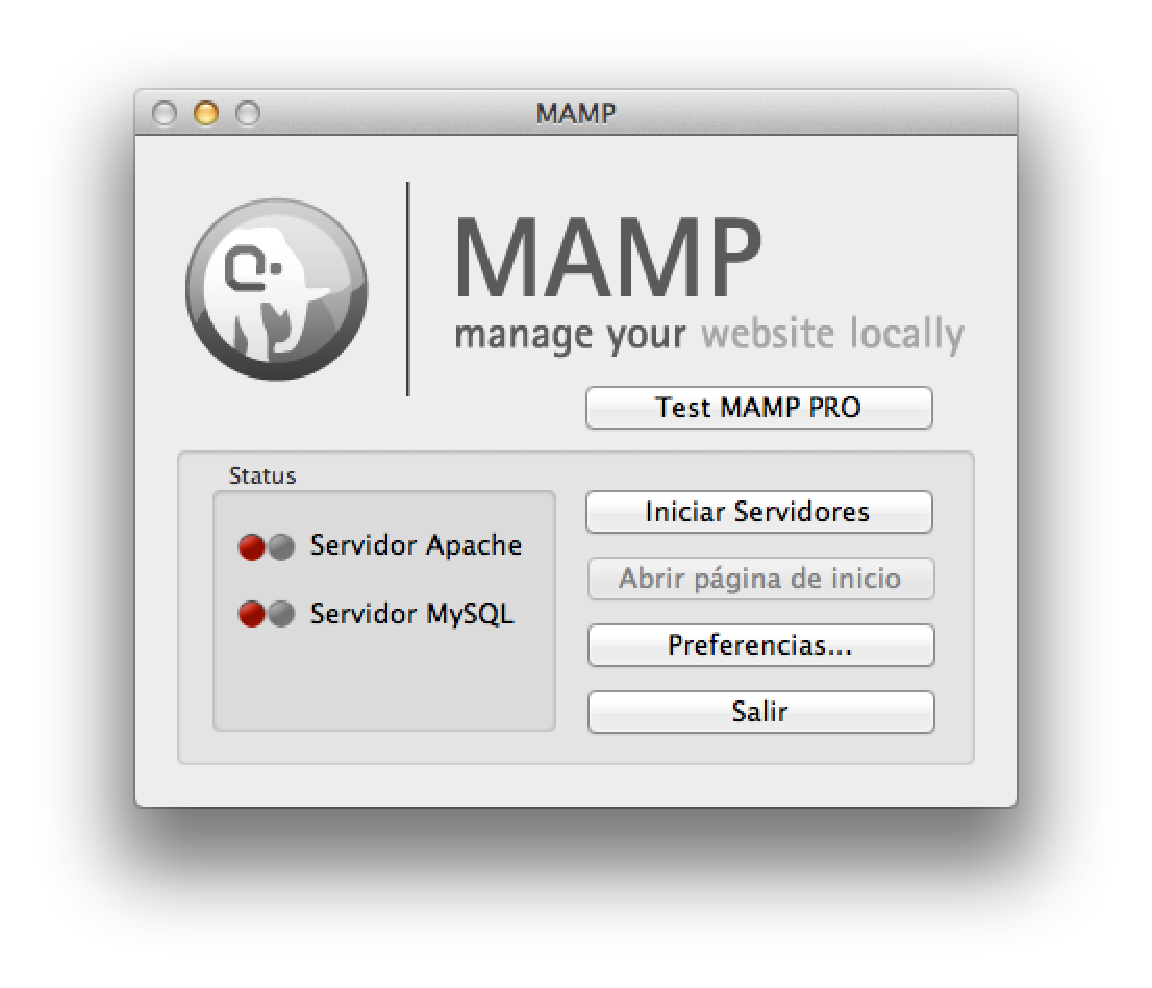
\includegraphics[width=\textwidth]{./img/wamp.eps}
	\caption{MAMP corriendo bajo Mac OS X}
\end{figure}

\subsection{Instalación del módulo \emph{mod-wikicode} en Moodle}

Puesto que el módulo que ha sido desarrollado en este proyecto está disponible tanto para la versión 1.x como para la 2.x de Moodle, a continuación se describe como instalarlo en dichas versiones.

\subsubsection{Instalación en Moodle 1.x}

En nuestro directorio del módulo tendremos las siguientes carpetas:  \emph{./lang} y  \emph{./mod}. Será necesario copiar los archivos en el interior de estos directorios a la ruta de nuestra instalación de nuestra instalación  \emph{Moodle}.

Una vez hayamos copiado estos archivos, haremos login como usuario administrador en Moodle y pulsaremos el botón Notifications:

\vspace{1cm}

\begin{figure}[h]
	\label{Notifications1x.eps}
	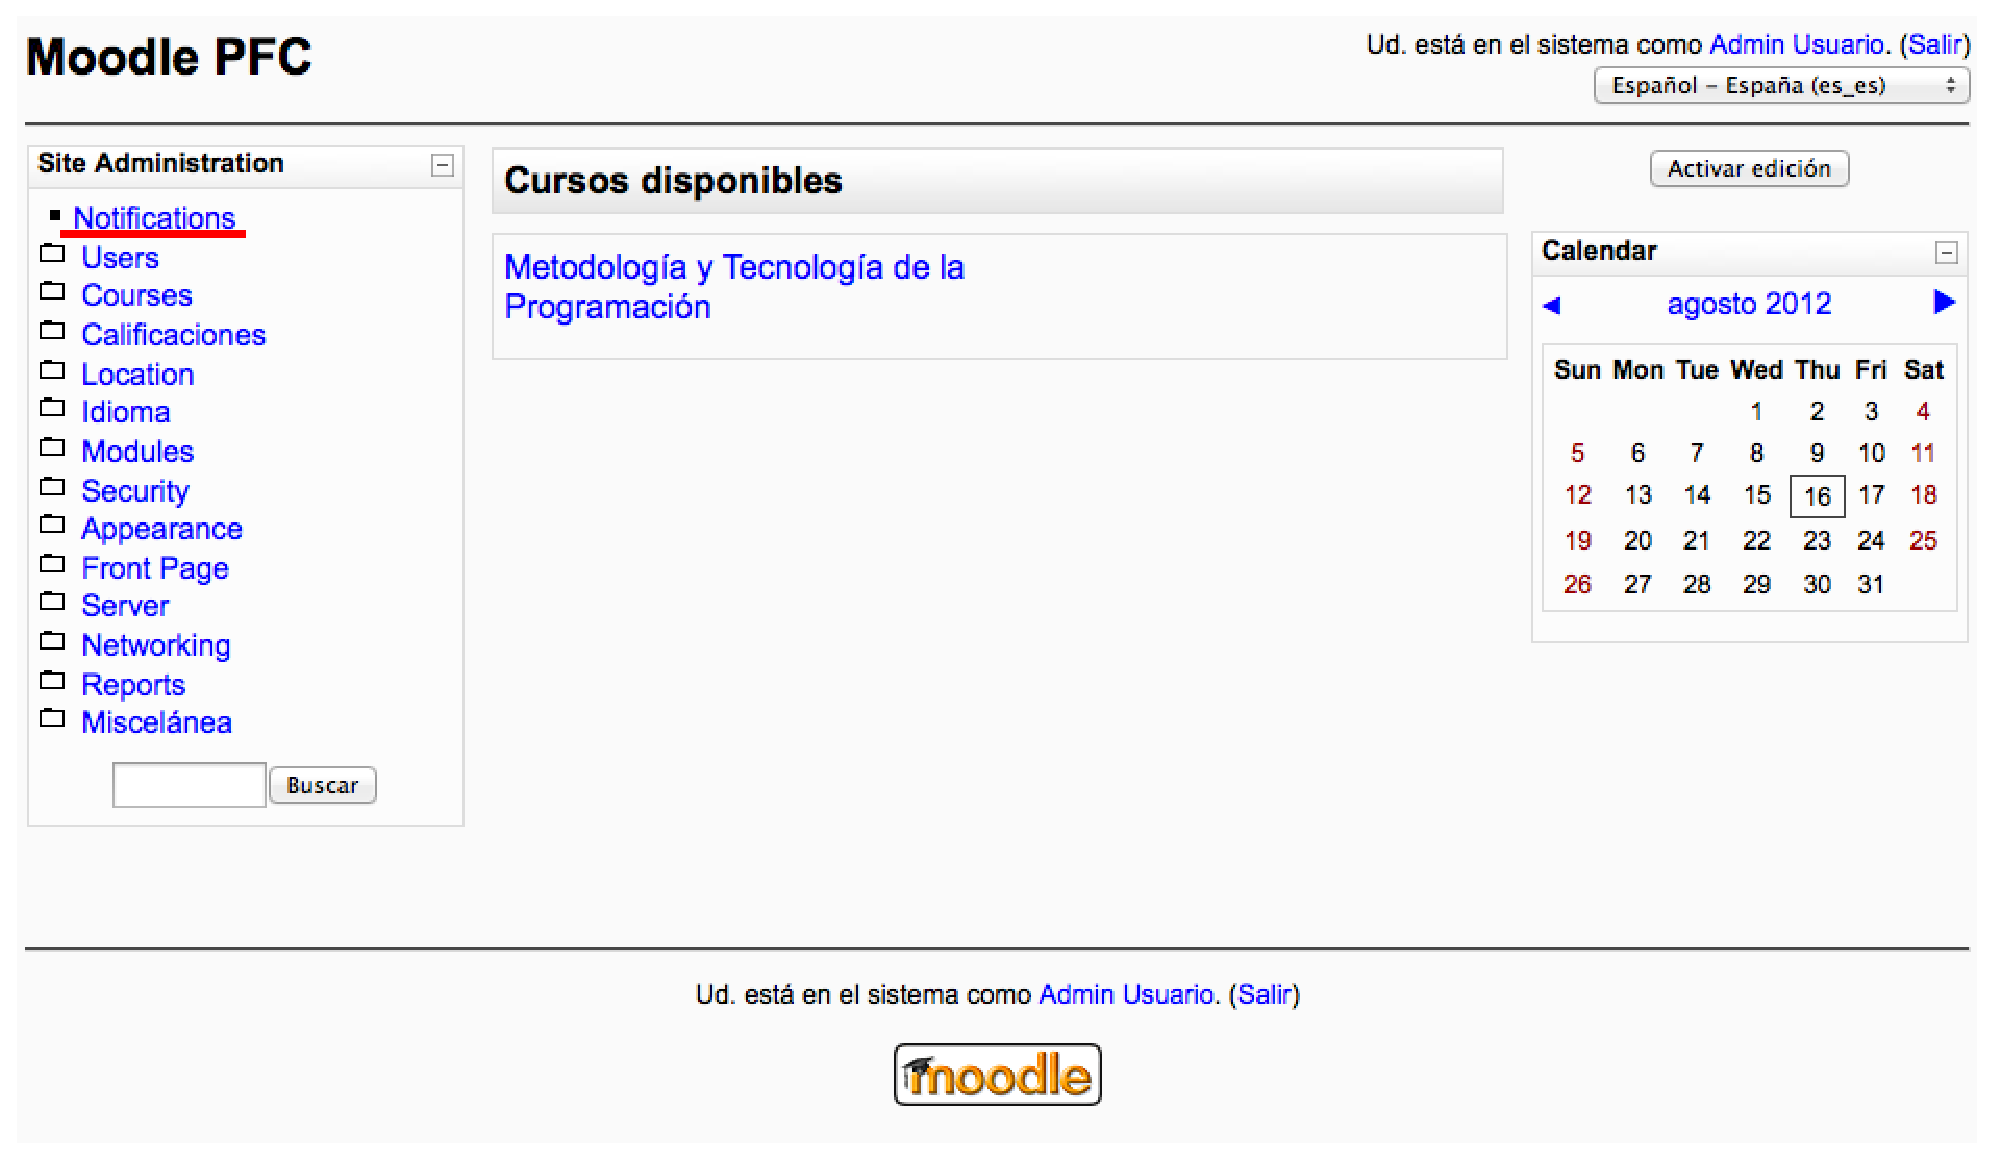
\includegraphics[width=\textwidth]{./img/Notifications1x.eps}
	\caption{Pantalla principal del administrador en Moodle 1.x}
\end{figure}

El sistema Moodle se encargará a partir de ese momento automáticamente de todo y el módulo quedará funcionalmente instalado.

\subsubsection{Instalación en Moodle 2.x}

En nuestro directorio del módulo tendremos únicamente una carpeta denominada \emph{/mod} y en su interior otra con el nombre \emph{/wikicode}. Simplemente tendremos que copiar esta última carpeta al directorio \emph{/mod} original de nuestro sistema Moodle. Una vez hayamos hecho esta copia bastará con hacer login como admin y todo se instalará automáticamente tras hacer las comprobaciones oportunas.

\begin{figure}[h]
	\label{installwikicode2x.eps}
	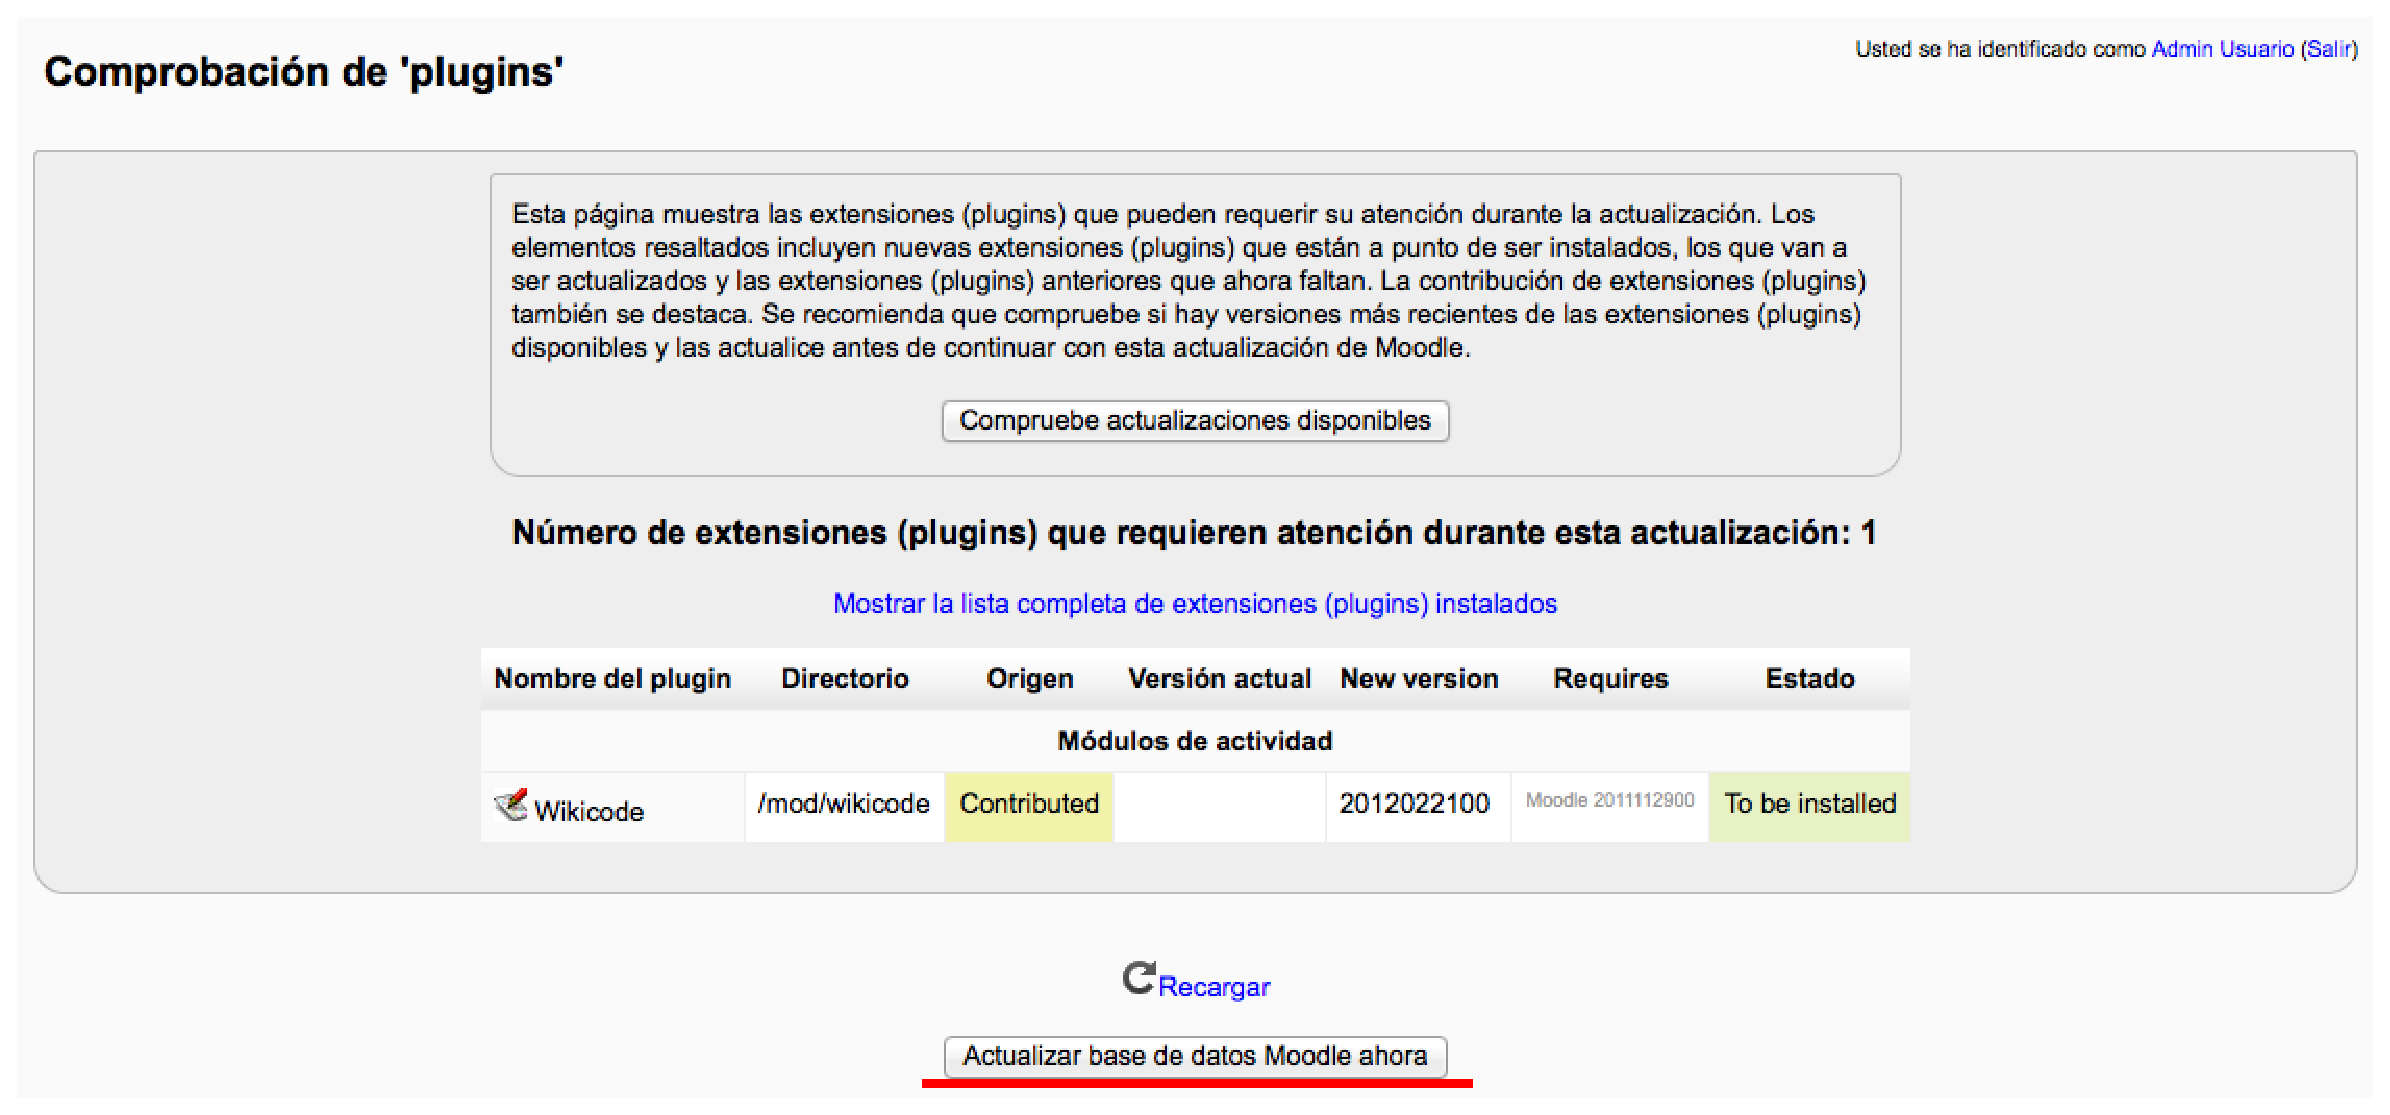
\includegraphics[width=\textwidth]{./img/installwikicode2x.eps}
	\caption{Instalación del módulo Wikicode en Moodle 2.x}
\end{figure}

\subsection{Actualización de JQuery}

Dentro de nuestro módulo, en el directorio \emph{/mod/wikicode/js}, tendremos un archivo denominado \textbf{jquery.js}. Esta archivo contiene la versión de \emph{JQuery 1.8.0}. Con esta versión todo funciona de modo correcto, pero si se quisiera actualizar con una versión futura para mejorar el rendimiento o añadir una nueva funcionalidad bastaría con actualizar dicho fichero.

\section{Desinstalación}

La desinstalación se trata de un proceso muy sencillo en nuestro caso. Puesto que tanto Moodle como el módulo funcionan con un intérprete, bastara con desinstalar nuestro conjunto de aplicaciones *AMP.

\subsection{Desinstalación en Windows. WampServer y MinGW.}
En primer lugar eliminaremos el servidor WAMP. Esta aplicación la podemos eliminar de dos maneras bastante simples: La primera es accediendo al Panel de Control, desde ahí seleccionamos \emph{"Agregar o Quitar Programas"} y lo marcamos para su correcta desinstalación. Un modo aún más sencillo es desde un terminal de Windows ejecutar el siguiente comando:

\begin{lstlisting}[style=consola]
	C:\Wamp\unins000.exe
\end{lstlisting}

Para desinstalar MinGW lo podemos hacer también desde la opción correspondiente dentro de \emph{"Agregar o Quitar Programas"}.
	
\subsection{Desinstalación en Mac OS. MAMP. }
Su desinstalación será bastante simple. Nos bastará con arrastrar la carpeta creada en el directorio Aplicaciones a la Papelera del sistema. Tras vaciar la Papelera se habrá eliminado la aplicación por completo.
	
\subsection{Desinstalación en GNU/Linux. Lamp Server y MinGW.}
Desde el propio Gestor de Paquetes que hayamos utilizado para instalar las aplicaciones, buscamos de nuevo la aplicación y la marcamos para desinstalar. Confiramos la operación y el Sistema de Gestión de Paquetes se encargará de borrar todos los archivos.
	
	
	
	
	
	
	
	
	
	
	
	
	
	
	
	
	
	
	
	
	
	
	
	
	
	
	
	
	%!TEX root=./pfc.tex
\chapter[Módulo para Moodle 2.x]{\label{}
Módulo para Moodle 2.x}

\section{Front-End}

\subsection{admin.php}
\begin{lstlisting}[language=PHP]
<?php

/**
 * Delete wiki pages or versions
 *
 * This will show options for deleting wiki pages or purging page versions
 * If user have wiki:managewiki ability then only this page will show delete
 * options
 *
 * @package mod-wikicode
 * @license http://www.gnu.org/copyleft/gpl.html GNU GPL v3 or later
 */

require_once('../../config.php');
require_once($CFG->dirroot . '/mod/wikicode/lib.php');
require_once($CFG->dirroot . '/mod/wikicode/locallib.php');
require_once($CFG->dirroot . '/mod/wikicode/pagelib.php');

$pageid = required_param('pageid', PARAM_INT); // Page ID
$delete = optional_param('delete', 0, PARAM_INT); // ID of the page to be deleted.
$option = optional_param('option', 1, PARAM_INT); // Option ID
$listall = optional_param('listall', 0, PARAM_INT); // list all pages
$toversion = optional_param('toversion', 0, PARAM_INT); // max version to be deleted
$fromversion = optional_param('fromversion', 0, PARAM_INT); // min version to be deleted

if (!$page = wikicode_get_page($pageid)) {
    print_error('incorrectpageid', 'wikicode');
}
if (!$subwiki = wikicode_get_subwiki($page->subwikiid)) {
    print_error('incorrectsubwikiid', 'wikicode');
}
if (!$cm = get_coursemodule_from_instance("wikicode", $subwiki->wikiid)) {
    print_error('invalidcoursemodule');
}
$course = $DB->get_record('course', array('id' => $cm->course), '*', MUST_EXIST);
if (!$wiki = wikicode_get_wiki($subwiki->wikiid)) {
    print_error('incorrectwikiid', 'wikicode');
}

require_login($course->id, true, $cm);


$context = get_context_instance(CONTEXT_MODULE, $cm->id);
require_capability('mod/wikicode:managewiki', $context);
add_to_log($course->id, "wikicode", "admin", "admin.php?id=$cm->id", "$wiki->id");

//Delete page if a page ID to delete was supplied
if (!empty($delete) && confirm_sesskey()) {
    wikicode_delete_pages($context, $delete, $page->subwikiid);
    //when current wiki page is deleted, then redirect user to create that page, as
    //current pageid is invalid after deletion.
    if ($pageid == $delete) {
        $params = array('swid' => $page->subwikiid, 'title' => $page->title);
        $url = new moodle_url('/mod/wikicode/create.php', $params);
        redirect($url);
    }
}

//delete version if toversion and fromversion are set.
if (!empty($toversion) && !empty($fromversion) && confirm_sesskey()) {
    //make sure all versions should not be deleted...
    $versioncount = wikicode_count_wikicode_page_versions($pageid);
    $versioncount -= 1; //ignore version 0
    $totalversionstodelete = $toversion - $fromversion;
    $totalversionstodelete += 1; //added 1 as toversion should be included

    if (($totalversionstodelete >= $versioncount) || ($versioncount <= 1)) {
        print_error('incorrectdeleteversions', 'wikicode');
    } else {
        $versions = array();
        for ($i = $fromversion; $i <= $toversion; $i++) {
            //Add all version to deletion list which exist
            if (wikicode_get_wikicode_page_version($pageid, $i)) {
                array_push($versions, $i);
            }
        }
        $purgeversions[$pageid] = $versions;
        wikicode_delete_page_versions($purgeversions);
    }
}

//show actual page
$wikipage = new page_wikicode_admin($wiki, $subwiki, $cm);

$wikipage->set_page($page);
$wikipage->print_header();
$wikipage->set_view($option, empty($listall)?true:false);
$wikipage->print_content();

$wikipage->print_footer();
\end{lstlisting}

\subsection{comments.php}
\begin{lstlisting}[language=PHP]
<?php
require_once('../../config.php');

require_once($CFG->dirroot . '/mod/wikicode/lib.php');
require_once($CFG->dirroot . '/mod/wikicode/locallib.php');
require_once($CFG->dirroot . '/mod/wikicode/pagelib.php');

$pageid = required_param('pageid', PARAM_TEXT);

if (!$page = wikicode_get_page($pageid)) {
    print_error('incorrectpageid', 'wikicode');
}

if (!$subwiki = wikicode_get_subwiki($page->subwikiid)) {
    print_error('incorrectsubwikiid', 'wikicode');
}

if (!$wiki = wikicode_get_wiki($subwiki->wikiid)) {
    print_error('incorrectwikiid', 'wikicode');
}

if (!$cm = get_coursemodule_from_instance('wikicode', $wiki->id)) {
    print_error('invalidcoursemodule');
}

$course = $DB->get_record('course', array('id' => $cm->course), '*', MUST_EXIST);

require_login($course->id, true, $cm);

add_to_log($course->id, 'wikicode', 'comments', 'comments.php?id=' . $cm->id, $wiki->id);

/// Print the page header
$wikipage = new page_wikicode_comments($wiki, $subwiki, $cm);

$wikipage->set_page($page);

$wikipage->print_header();
$wikipage->print_content();
$wikipage->print_footer();
\end{lstlisting}

\subsection{comments\_form.php}
\begin{lstlisting}[language=PHP]
<?php

if (!defined('MOODLE_INTERNAL')) {
    die('Direct access to this script is forbidden.');    ///  It must be included from a Moodle page
}

require_once($CFG->dirroot . '/lib/formslib.php');

class mod_wikicode_comments_form extends moodleform {
    function definition() {
        $pageid = optional_param('pageid', 0, PARAM_INT);
        $mform =& $this->_form;

        $current = $this->_customdata['current'];
        $commentoptions = $this->_customdata['commentoptions'];

        // visible elements
        $mform->addElement('editor', 'entrycomment_editor', get_string('comment', 'glossary'), null, $commentoptions);
        $mform->addRule('entrycomment_editor', get_string('required'), 'required', null, 'client');
        $mform->setType('entrycomment_editor', PARAM_RAW); // processed by trust text or cleaned before the display

        // hidden optional params
        $mform->addElement('hidden', 'id', '');
        $mform->setType('id', PARAM_INT);

        $mform->addElement('hidden', 'action', '');
        $mform->setType('action', PARAM_ACTION);

        //-------------------------------------------------------------------------------
        // buttons
        $this->add_action_buttons(false);

        //-------------------------------------------------------------------------------
        $this->set_data($current);
    }

    public function edit_definition($current, $commentoptions) {
        $this->set_data($current);
        $this->set_data($commentoptions);
    }
}
\end{lstlisting}

\subsection{create.php}
\begin{lstlisting}[language=PHP]
<?php

require_once('../../config.php');
require_once(dirname(__FILE__) . '/create_form.php');
require_once($CFG->dirroot . '/mod/wikicode/lib.php');
require_once($CFG->dirroot . '/mod/wikicode/locallib.php');
require_once($CFG->dirroot . '/mod/wikicode/pagelib.php');

// this page accepts two actions: new and create
// 'new' action will display a form contains page title and page format
// selections
// 'create' action will create a new page in db, and redirect to
// page editing page.
$action = optional_param('action', 'new', PARAM_TEXT);
// The title of the new page, can be empty
$title = optional_param('title', '', PARAM_TEXT);
$wid = optional_param('wid', 0, PARAM_INT);
$swid = optional_param('swid', 0, PARAM_INT);
$gid = optional_param('gid', 0, PARAM_INT);
$uid = optional_param('uid', 0, PARAM_INT);

// 'create' action must be submitted by moodle form
// so sesskey must be checked
if ($action == 'create') {
    if (!confirm_sesskey()) {
        print_error('invalidsesskey');
    }
}

if (!empty($swid)) {
    $subwiki = wikicode_get_subwiki($swid);

    if (!$wiki = wikicode_get_wiki($subwiki->wikiid)) {
        print_error('invalidwikiid', 'wikicode');
    }

} else {
    $subwiki = wikicode_get_subwiki_by_group($wid, $gid, $uid);

    if (!$wiki = wikicode_get_wiki($wid)) {
        print_error('invalidwikiid', 'wikicode');
    }

}

if (!$cm = get_coursemodule_from_instance('wikicode', $wiki->id)) {
    print_error('invalidcoursemoduleid', 'wikicode');
}

$course = $DB->get_record('course', array('id' => $cm->course), '*', MUST_EXIST);

require_login($course->id, true, $cm);

add_to_log($course->id, 'createpage', 'createpage', 'view.php?id=' . $cm->id, $wiki->id);

$wikipage = new page_wikicode_create($wiki, $subwiki, $cm);

if (!empty($swid)) {
    $wikipage->set_gid($subwiki->groupid);
    $wikipage->set_uid($subwiki->userid);
    $wikipage->set_swid($swid);
} else {
    $wikipage->set_wid($wid);
    $wikipage->set_gid($gid);
    $wikipage->set_uid($uid);
}

if (!empty($title)) {
    $wikipage->set_title($title);
} else {
    $wikipage->set_title(get_string('newpage', 'wikicode'));
}

// set page action, and initialise moodle form
$wikipage->set_action($action);

switch ($action) {
case 'create':
    $wikipage->create_page($title);
    break;
case 'new':
    if ((int)$wiki->forceformat == 1 && !empty($title)) {
        $wikipage->create_page($title);
    } else {
        // create link from moodle navigation block without pagetitle
        $wikipage->print_header();
        // new page without page title
        $wikipage->print_content($title);
    }
    $wikipage->print_footer();
    break;
}
\end{lstlisting}

\subsection{create\_form.php}
\begin{lstlisting}[language=PHP]
<?php

require_once($CFG->libdir.'/formslib.php');

class mod_wikicode_create_form extends moodleform {

    protected function definition() {
        global $CFG;
        $mform =& $this->_form;

        $formats = $this->_customdata['formats'];
        $defaultformat = $this->_customdata['defaultformat'];
        $forceformat = $this->_customdata['forceformat'];

        $mform->addElement('header', 'general', get_string('createpage', 'wikicode'));

        $textoptions = array();
        if (!empty($this->_customdata['disable_pagetitle'])) {
            $textoptions = array('readonly'=>'readonly');
        }
        $mform->addElement('text', 'pagetitle', get_string('newpagetitle', 'wikicode'), $textoptions);

        if ($forceformat) {
            $mform->addElement('hidden', 'pageformat', $defaultformat);
        } else {
            $mform->addElement('static', 'format', get_string('format', 'wikicode'));
            $mform->addHelpButton('format', 'format', 'wikicode');
            foreach ($formats as $format) {
                if ($format == $defaultformat) {
                    $attr = array('checked'=>'checked');
                }else if (!empty($forceformat)){
                    $attr = array('disabled'=>'disabled');
                } else {
                    $attr = array();
                }
                $mform->addElement('radio', 'pageformat', '', get_string('format'.$format, 'wikicode'), $format, $attr);
            }
        }

        //hiddens
        $mform->addElement('hidden', 'action');
        $mform->setDefault('action', 'create');

        $this->add_action_buttons(false, get_string('createpage', 'wikicode'));
    }
}
\end{lstlisting}

\subsection{diff.php}
\begin{lstlisting}[language=PHP]
<?php

require_once('../../config.php');

require_once($CFG->dirroot . '/mod/wikicode/lib.php');
require_once($CFG->dirroot . '/mod/wikicode/locallib.php');
require_once($CFG->dirroot . '/mod/wikicode/pagelib.php');

require_once($CFG->dirroot . '/mod/wikicode/diff/difflib.php');
require_once($CFG->dirroot . '/mod/wikicode/diff/diff_nwiki.php');

$pageid = required_param('pageid', PARAM_TEXT);
$compare = required_param('compare', PARAM_INT);
$comparewith = required_param('comparewith', PARAM_INT);

if (!$page = wikicode_get_page($pageid)) {
    print_error('incorrectpageid', 'wikicode');
}

if (!$subwiki = wikicode_get_subwiki($page->subwikiid)) {
    print_error('incorrectsubwikiid', 'wikicode');
}

if (!$wiki = wikicode_get_wiki($subwiki->wikiid)) {
    print_error('incorrectwikiid', 'wikicode');
}

if (!$cm = get_coursemodule_from_instance('wikicode', $wiki->id)) {
    print_error('invalidcoursemodule');
}

$course = $DB->get_record('course', array('id' => $cm->course), '*', MUST_EXIST);

if ($compare >= $comparewith) {
    print_error("A page version can only be compared with an older version.");
}

require_login($course->id, true, $cm);
add_to_log($course->id, "wikicode", "diff", "diff.php?id=$cm->id", "$wiki->id");

$wikipage = new page_wikicode_diff($wiki, $subwiki, $cm);

$wikipage->set_page($page); 
$wikipage->set_comparison($compare, $comparewith);

$wikipage->print_header();

$wikipage->print_content();

$wikipage->print_footer();
\end{lstlisting}

\subsection{edit.php}
\begin{lstlisting}[language=PHP]
<?php

require_once('../../config.php');

require_once($CFG->dirroot . '/mod/wikicode/lib.php');
require_once($CFG->dirroot . '/mod/wikicode/locallib.php');
require_once($CFG->dirroot . '/mod/wikicode/pagelib.php');

$pageid = required_param('pageid', PARAM_INT);
$contentformat = optional_param('contentformat', '', PARAM_ALPHA);
$option = optional_param('editoption', '', PARAM_TEXT);
$section = optional_param('section', "", PARAM_TEXT);
$version = optional_param('version', -1, PARAM_INT);
$attachments = optional_param('attachments', 0, PARAM_INT);
$deleteuploads = optional_param('deleteuploads', 0, PARAM_RAW);
$compiled = optional_param('compiled', 0, PARAM_INT);

$newcontent = '';
if (!empty($newcontent) && is_array($newcontent)) {
    $newcontent = $newcontent['text'];
} 

if (!empty($option) && is_array($option)) {
    $option = $option['editoption'];
}

if (!$page = wikicode_get_page($pageid)) {
    print_error('incorrectpageid', 'wikicode');
}

if (!$subwiki = wikicode_get_subwiki($page->subwikiid)) {
    print_error('incorrectsubwikiid', 'wikicode');
}

if (!$wiki = wikicode_get_wiki($subwiki->wikiid)) {
    print_error('incorrectwikiid', 'wikicode');
}

if (!$cm = get_coursemodule_from_instance('wikicode', $wiki->id)) {
    print_error('invalidcoursemodule');
}

$course = $DB->get_record('course', array('id' => $cm->course), '*', MUST_EXIST);

if (!empty($section) && !$sectioncontent = wikicode_get_section_page($page, $section)) {
    print_error('invalidsection', 'wikicode');
}

require_login($course, true, $cm);

$context = get_context_instance(CONTEXT_MODULE, $cm->id);
require_capability('mod/wikicode:editpage', $context);

add_to_log($course->id, 'wikicode', 'edit', "edit.php?id=$cm->id", "$wiki->id");

if ($option == get_string('save', 'wikicode')) {
    if (!confirm_sesskey()) {
        print_error(get_string('invalidsesskey', 'wikicode'));
    }
    $wikipage = new page_wikicode_save($wiki, $subwiki, $cm);
    $wikipage->set_page($page);
    $wikipage->set_newcontent($newcontent);
    $wikipage->set_upload(true);
} else {  
    if ($option == 'Compile' or $option == 'Download') {
        if (!confirm_sesskey()) {
            print_error(get_string('invalidsesskey', 'wikicode'));
        }
        $wikipage = new page_wikicode_compile($wiki, $subwiki, $cm);
        $wikipage->set_page($page);
		$wikipage->set_download(($option == 'Download'));
    }
	else {
        if ($option == get_string('cancel')) {
            //delete lock
            wikicode_delete_locks($page->id, $USER->id, $section);

            redirect($CFG->wwwroot . '/mod/wikicode/view.php?pageid=' . $pageid);
        } else {
            $wikipage = new page_wikicode_edit($wiki, $subwiki, $cm);
            $wikipage->set_page($page);
            $wikipage->set_upload($option == get_string('upload', 'wikicode'));
			$wikipage->set_compiled($compiled);
        }
    }

    if (has_capability('mod/wikicode:overridelock', $context)) {
        $wikipage->set_overridelock(true);
    }
}

if ($version >= 0) {
    $wikipage->set_versionnumber($version);
}

if (!empty($section)) {
    $wikipage->set_section($sectioncontent, $section);
}

if (!empty($attachments)) {
    $wikipage->set_attachments($attachments);
}

if (!empty($deleteuploads)) {
    $wikipage->set_deleteuploads($deleteuploads);
}

if (!empty($contentformat)) {
    $wikipage->set_format($contentformat);
}

$wikipage->print_header();

$wikipage->print_content();

$wikipage->print_footer();
\end{lstlisting}

\subsection{edit\_form.php}
\begin{lstlisting}[language=PHP]
<?php

if (!defined('MOODLE_INTERNAL')) {
    die('Direct access to this script is forbidden.');    ///  It must be included from a Moodle page
}

require_once($CFG->dirroot . '/mod/wikicode/editors/wikieditor.php');
require_once($CFG->dirroot . '/mod/wikicode/chat/wikichat.php');

class mod_wikicode_edit_form extends moodleform {

    protected function definition() {
        global $CFG, $USER, $DB;

        $mform =& $this->_form;

        $version = $this->_customdata['version'];
        $format  = $this->_customdata['format'];
        $tags    = !isset($this->_customdata['tags'])?"":$this->_customdata['tags'];

        if ($format != 'html') {
            $contextid  = $this->_customdata['contextid'];
            $filearea   = $this->_customdata['filearea'];
            $fileitemid = $this->_customdata['fileitemid'];
        }

        if (isset($this->_customdata['pagetitle'])) {
            $pagetitle = get_string('editingpage', 'wikicode', $this->_customdata['pagetitle']);
        } else {
            $pagetitle = get_string('editing', 'wikicode');
        }

        //editor
        $mform->addElement('header', 'general', $pagetitle);

        $fieldname = get_string('format' . $format, 'wikicode');
        if ($format != 'html') {
            // Use wiki editor
            $extensions = file_get_typegroup('extension', 'web_image');
            $fs = get_file_storage();
            $tree = $fs->get_area_tree($contextid, 'mod_wikicode', 'attachments', $fileitemid);
            $files = array();
            foreach ($tree['files'] as $file) {
                $filename = $file->get_filename();
                foreach ($extensions as $ext) {
                    if (preg_match('#'.$ext.'$#i', $filename)) {
                        $files[] = $filename;
                    }
                }
            }
			$buttoncommands=array();
			$buttoncommands[] =& $mform->createElement('button','editoption','Unlock', array('id' => 'btnunlock', 'class' => 'btnunlock'));
			$buttoncommands[] =& $mform->createElement('button','editoption','Refresh', array('id' => 'btnref', 'class' => 'btnref'));
			$buttoncommands[] =& $mform->createElement('submit', 'editoption', 'Save', array('id' => 'save'));
			$mform->addGroup($buttoncommands, 'editoption', 'Actions:', '', true);
            $mform->addElement('wikicodeeditor', 'newcontent', $fieldname, array('cols' => 150, 'rows' => 30, 'Wiki_format' => $format, 'files'=>$files));
        } else {
            $mform->addElement('editor', 'newcontent_editor', $fieldname, null, page_wikicode_edit::$attachmentoptions);
            $mform->addHelpButton('newcontent_editor', 'formathtml', 'wikicode');
        }
		
		//chat
		$mform->addElement('header','chat','Chat');
		$mform->addElement('wikicodechat', 'wikicodechat', null, array('itemid'=>$fileitemid));
		
		//compiler
		$mform->addElement('header','compiler', 'Compiler');
		$mform->addElement('textarea', 'textCompiler', '', 'wrap="virtual" rows="3" cols="150" readonly="readonly" ');
		//$mform->addElement('submit','editoption','Compilar', array('id' => 'compile'));
		//$mform->addElement('submit','editoption','Descargar', array('id' => 'download'));
		
		$buttonarray=array();
		$buttonarray[] =& $mform->createElement('submit','editoption','Compile', array('id' => 'compile'));
		$buttonarray[] =& $mform->createElement('submit','editoption','Download', array('id' => 'compile'));
		$mform->addGroup($buttonarray, 'editoption', 'Options:', '', true);

        //hiddens
        if ($version >= 0) {
            $mform->addElement('hidden', 'version');
            $mform->setDefault('version', $version);
        }

        $mform->addElement('hidden', 'contentformat');
        $mform->setDefault('contentformat', $format);
		
		$mform->addElement('hidden', 'insert');
		$mform->setDefault('insert', 1);

    }

}
\end{lstlisting}

\subsection{files.php}
\begin{lstlisting}[language=PHP]
<?php
require_once('../../config.php');
require_once($CFG->dirroot . '/mod/wikicode/lib.php');
require_once($CFG->dirroot . '/mod/wikicode/locallib.php');

$pageid       = required_param('pageid', PARAM_INT); // Page ID
$wid          = optional_param('wid', 0, PARAM_INT); // Wiki ID
$currentgroup = optional_param('group', 0, PARAM_INT); // Group ID
$userid       = optional_param('uid', 0, PARAM_INT); // User ID
$groupanduser = optional_param('groupanduser', null, PARAM_TEXT);

if (!$page = wikicode_get_page($pageid)) {
    print_error('incorrectpageid', 'wikicode');
}

if ($groupanduser) {
    list($currentgroup, $userid) = explode('-', $groupanduser);
    $currentgroup = clean_param($currentgroup, PARAM_INT);
    $userid       = clean_param($userid, PARAM_INT);
}

if ($wid) {
    // in group mode
    if (!$wiki = wikicode_get_wiki($wid)) {
        print_error('incorrectwikiid', 'wikicode');
    }
    if (!$subwiki = wikicode_get_subwiki_by_group($wiki->id, $currentgroup, $userid)) {
        // create subwiki if doesn't exist
        $subwikiid = wikicode_add_subwiki($wiki->id, $currentgroup, $userid);
        $subwiki = wikicode_get_subwiki($subwikiid);
    }
} else {
    // no group
    if (!$subwiki = wikicode_get_subwiki($page->subwikiid)) {
        print_error('incorrectsubwikiid', 'wikicode');
    }

    // Checking wiki instance of that subwiki
    if (!$wiki = wikicode_get_wiki($subwiki->wikiid)) {
        print_error('incorrectwikiid', 'wikicode');
    }
}

// Checking course module instance
if (!$cm = get_coursemodule_from_instance("wikicode", $subwiki->wikiid)) {
    print_error('invalidcoursemodule');
}

// Checking course instance
$course = $DB->get_record('course', array('id' => $cm->course), '*', MUST_EXIST);

$context = get_context_instance(CONTEXT_MODULE, $cm->id);


$PAGE->set_url('/mod/wikicode/files.php', array('pageid'=>$pageid));
require_login($course, true, $cm);
$PAGE->set_context($context);
$PAGE->set_title(get_string('wikifiles', 'wikicode'));
$PAGE->set_heading(get_string('wikifiles', 'wikicode'));
$PAGE->navbar->add(format_string(get_string('wikifiles', 'wikicode')));
echo $OUTPUT->header();

$renderer = $PAGE->get_renderer('mod_wikicode');

$tabitems = array('view' => 'view', 'edit' => 'edit', 'comments' => 'comments', 'history' => 'history', 'map' => 'map', 'files' => 'files');

$options = array('activetab'=>'files');
echo $renderer->tabs($page, $tabitems, $options);


echo $OUTPUT->box_start('generalbox');
if (has_capability('mod/wikicode:viewpage', $context)) {
    echo $renderer->wikicode_print_subwiki_selector($PAGE->activityrecord, $subwiki, $page, 'files');
    echo $renderer->wikicode_files_tree($context, $subwiki);
} else {
    echo $OUTPUT->notification(get_string('cannotviewfiles', 'wikicode'));
}
echo $OUTPUT->box_end();

if (has_capability('mod/wikicode:managefiles', $context)) {
    echo $OUTPUT->single_button(new moodle_url('/mod/wikicode/filesedit.php', array('subwiki'=>$subwiki->id, 'pageid'=>$pageid)), get_string('editfiles', 'wikicode'), 'get');
}
echo $OUTPUT->footer();
\end{lstlisting}

\subsection{filesedit.php}
\begin{lstlisting}[language=PHP]
<?php

/**
 * Manage files in wiki
 *
 * @package   mod-wikicode
 * @copyright 2011 Dongsheng Cai <dongsheng@moodle.com>
 * @license   http://www.gnu.org/copyleft/gpl.html GNU GPL v3 or later
 */

require_once(dirname(dirname(dirname(__FILE__))) . '/config.php');
require_once('lib.php');
require_once('locallib.php');
require_once("$CFG->dirroot/mod/wikicode/filesedit_form.php");
require_once("$CFG->dirroot/repository/lib.php");

$subwikiid = required_param('subwiki', PARAM_INT);
// not being used for file management, we use it to generate navbar link
$pageid    = optional_param('pageid', 0, PARAM_INT);
$returnurl = optional_param('returnurl', '', PARAM_URL);

if (!$subwiki = wikicode_get_subwiki($subwikiid)) {
    print_error('incorrectsubwikiid', 'wikicode');
}

// Checking wiki instance of that subwiki
if (!$wiki = wikicode_get_wiki($subwiki->wikiid)) {
    print_error('incorrectwikiid', 'wikicode');
}

// Checking course module instance
if (!$cm = get_coursemodule_from_instance("wikicode", $subwiki->wikiid)) {
    print_error('invalidcoursemodule');
}

// Checking course instance
$course = $DB->get_record('course', array('id' => $cm->course), '*', MUST_EXIST);

$context = get_context_instance(CONTEXT_MODULE, $cm->id);

require_login($course, true, $cm);
require_capability('mod/wikicode:managefiles', $context);

if (empty($returnurl)) {
    if (!empty($_SERVER["HTTP_REFERER"])) {
        $returnurl = $_SERVER["HTTP_REFERER"];
    } else {
        $returnurl = new moodle_url('/mod/wikicode/files.php', array('subwiki'=>$subwiki->id));
    }
}

$title = get_string('editfiles', 'wikicode');

$struser = get_string('user');
$url = new moodle_url('/mod/wikicode/filesedit.php', array('subwiki'=>$subwiki->id, 'pageid'=>$pageid));
$PAGE->set_url($url);
$PAGE->set_context($context);
$PAGE->set_title($title);
$PAGE->set_heading($title);
$PAGE->navbar->add(format_string(get_string('wikifiles', 'wikicode')), $CFG->wwwroot . '/mod/wikicode/files.php?pageid=' . $pageid);
$PAGE->navbar->add(format_string($title));

$data = new stdClass();
$data->returnurl = $returnurl;
$data->subwikiid = $subwiki->id;
$maxbytes = get_max_upload_file_size($CFG->maxbytes, $COURSE->maxbytes);
$options = array('subdirs'=>0, 'maxbytes'=>$maxbytes, 'maxfiles'=>-1, 'accepted_types'=>'*', 'return_types'=>FILE_INTERNAL);
file_prepare_standard_filemanager($data, 'files', $options, $context, 'mod_wiki', 'attachments', $subwiki->id);

$mform = new mod_wikicode_filesedit_form(null, array('data'=>$data, 'options'=>$options));

if ($mform->is_cancelled()) {
    redirect($returnurl);
} else if ($formdata = $mform->get_data()) {
    $formdata = file_postupdate_standard_filemanager($formdata, 'files', $options, $context, 'mod_wikicode', 'attachments', $subwiki->id);
    redirect($returnurl);
}

echo $OUTPUT->header();
echo $OUTPUT->box_start('generalbox');
$mform->display();
echo $OUTPUT->box_end();
echo $OUTPUT->footer();
\end{lstlisting}

\subsection{filesedit\_form.php}
\begin{lstlisting}[language=PHP]
<?php

/**
 * Edit wiki files form
 *
 * @package   mod-wikicode
 * @copyright 2011 Dongsheng Cai <dongsheng@moodle.com>
 * @license   http://www.gnu.org/copyleft/gpl.html GNU GPL v3 or later
 */

defined('MOODLE_INTERNAL') || die();

require_once("$CFG->libdir/formslib.php");

class mod_wikicode_filesedit_form extends moodleform {
    function definition() {
        $mform = $this->_form;

        $data    = $this->_customdata['data'];
        $options = $this->_customdata['options'];

        $mform->addElement('filemanager', 'files_filemanager', get_string('files'), null, $options);
        $mform->addElement('hidden', 'returnurl', $data->returnurl);
        $mform->addElement('hidden', 'subwiki', $data->subwikiid);

        $this->add_action_buttons(true, get_string('savechanges'));

        $this->set_data($data);
    }
}
\end{lstlisting}

\subsection{history.php}
\begin{lstlisting}[language=PHP]
<?php

require_once('../../config.php');

require_once($CFG->dirroot . '/mod/wikicode/lib.php');
require_once($CFG->dirroot . '/mod/wikicode/locallib.php');
require_once($CFG->dirroot . '/mod/wikicode/pagelib.php');

$pageid = required_param('pageid', PARAM_TEXT);
$paging = optional_param('page', 0, PARAM_INT);
$allversion = optional_param('allversion', 0, PARAM_INT);

if (!$page = wikicode_get_page($pageid)) {
    print_error('incorrectpageid', 'wikicode');
}

if (!$subwiki = wikicode_get_subwiki($page->subwikiid)) {
    print_error('incorrectsubwikiid', 'wikicode');
}

if (!$wiki = wikicode_get_wiki($subwiki->wikiid)) {
    print_error('incorrectwikiid', 'wikicode');
}

if (!$cm = get_coursemodule_from_instance('wikicode', $wiki->id)) {
    print_error('invalidcoursemodule');
}

$course = $DB->get_record('course', array('id' => $cm->course), '*', MUST_EXIST);

require_login($course->id, true, $cm);
$context = get_context_instance(CONTEXT_MODULE, $cm->id);
require_capability('mod/wikicode:viewpage', $context);
add_to_log($course->id, 'wikicode', 'history', 'history.php?id=' . $cm->id, $wiki->id);

/// Print the page header
$wikipage = new page_wikicode_history($wiki, $subwiki, $cm);

$wikipage->set_page($page);
$wikipage->set_paging($paging);
$wikipage->set_allversion($allversion);

$wikipage->print_header();
$wikipage->print_content();

$wikipage->print_footer();
\end{lstlisting}

\subsection{index.php}
\begin{lstlisting}[language=PHP]
<?php

require_once('../../config.php');
require_once('lib.php');

$id = required_param('id', PARAM_INT); // course
$PAGE->set_url('/mod/wikicode/index.php', array('id' => $id));

if (!$course = $DB->get_record('course', array('id' => $id))) {
    print_error('invalidcourseid');
}

require_login($course->id, true);
$PAGE->set_pagelayout('incourse');
$context = get_context_instance(CONTEXT_COURSE, $course->id);

add_to_log($course->id, 'wikicode', 'view all', "index.php?id=$course->id", "");

/// Get all required stringswiki
$strwikis = get_string("modulenameplural", "wikicode");
$strwiki = get_string("modulename", "wikicode");

/// Print the header
$PAGE->navbar->add($strwikis, "index.php?id=$course->id");
$PAGE->set_title($strwikis);
$PAGE->set_heading($course->fullname);
echo $OUTPUT->header();

/// Get all the appropriate data
if (!$wikis = get_all_instances_in_course("wikicode", $course)) {
    notice("There are no wikis", "../../course/view.php?id=$course->id");
    die;
}

$usesections = course_format_uses_sections($course->format);
if ($usesections) {
    $sections = get_all_sections($course->id);
}

/// Print the list of instances (your module will probably extend this)

$timenow = time();
$strsectionname = get_string('sectionname', 'format_' . $course->format);
$strname = get_string("name");
$table = new html_table();

if ($usesections) {
    $table->head = array($strsectionname, $strname);
} else {
    $table->head = array($strname);
}

foreach ($wikis as $wiki) {
    $linkcss = null;
    if (!$wiki->visible) {
        $linkcss = array('class' => 'dimmed');
    }
    $link = html_writer::link(new moodle_url('/mod/wikicode/view.php', array('id' => $wiki->coursemodule)), $wiki->name, $linkcss);

    if ($usesections) {
        $table->data[] = array(get_section_name($course, $sections[$wiki->section]), $link);
    } else {
        $table->data[] = array($link);
    }
}

echo html_writer::table($table);

/// Finish the page
echo $OUTPUT->footer();
\end{lstlisting}

\subsection{log.php}
\begin{lstlisting}[language=PHP]
<?php

require_once('../../config.php');

require_once($CFG->dirroot . '/mod/wikicode/lib.php');
require_once($CFG->dirroot . '/mod/wikicode/locallib.php');
require_once($CFG->dirroot . '/mod/wikicode/pagelib.php');

$pageid = required_param('pageid', PARAM_INT);
$section = optional_param('section', "", PARAM_TEXT);
$version = optional_param('version', -1, PARAM_INT);

if (!$page = wikicode_get_page($pageid)) {
    print_error('incorrectpageid', 'wikicode');
}

if (!$subwiki = wikicode_get_subwiki($page->subwikiid)) {
    print_error('incorrectsubwikiid', 'wikicode');
}

if (!$wiki = wikicode_get_wiki($subwiki->wikiid)) {
    print_error('incorrectwikiid', 'wikicode');
}

if (!$cm = get_coursemodule_from_instance('wikicode', $wiki->id)) {
    print_error('invalidcoursemodule');
}

$course = $DB->get_record('course', array('id' => $cm->course), '*', MUST_EXIST);

if (!empty($section) && !$sectioncontent = wikicode_get_section_page($page, $section)) {
    print_error('invalidsection', 'wikicode');
}

require_login($course, true, $cm);

$context = get_context_instance(CONTEXT_MODULE, $cm->id);
require_capability('mod/wikicode:editpage', $context);

add_to_log($course->id, 'wikicode', 'log', "log.php?id=$cm->id", "$wiki->id");

$wikipage = new page_wikicode_log($wiki, $subwiki, $cm);
$wikipage->set_page($page);

$wikipage->print_header();

$wikipage->print_content();

$wikipage->print_footer();
\end{lstlisting}

\subsection{log\_form.php}
\begin{lstlisting}[language=PHP]
<?php

if (!defined('MOODLE_INTERNAL')) {
    die('Direct access to this script is forbidden.');    ///  It must be included from a Moodle page
}

class mod_wikicode_log_form extends moodleform {

    protected function definition() {
        global $CFG, $USER, $DB;

        $mform =& $this->_form;

        $version = $this->_customdata['version'];
        $format  = $this->_customdata['format'];
        $tags    = !isset($this->_customdata['tags'])?"":$this->_customdata['tags'];

        if ($format != 'html') {
            $contextid  = $this->_customdata['contextid'];
            $filearea   = $this->_customdata['filearea'];
            $fileitemid = $this->_customdata['fileitemid'];
        }

        if (isset($this->_customdata['pagetitle'])) {
            $pagetitle = get_string('logpage', 'wikicode', $this->_customdata['pagetitle']);
        } else {
            $pagetitle = get_string('loging', 'wikicode');
        }
		
		//Time
		$time = $this->_customdata['page']->timeendedit - $this->_customdata['page']->timestartedit;
		$seconds = $time % 60;
		$time = ($time - $seconds) / 60;
		$minutes = $time % 60;
		$hours = ($time - $minutes) / 60;		
		
		//Stats
		$attr = array('size' => '75', 'readonly' => 1);
		$mform->addElement('header','stats', 'Stats');
		$attr['value'] = $hours . " hours, " . $minutes . " minutes, " . $seconds . " seconds";
		$mform->addElement('text', 'timeedit', 'Editing Time', $attr);
		$mform->addHelpButton('timeedit', 'timeedit', 'wikicode');
		$attr['value'] = $this->_customdata['page']->errorcompile;
		$mform->addElement('text', 'errorscompilation', 'Compilation Errors', $attr);
		$mform->addHelpButton('errorscompilation', 'errorscompilation', 'wikicode');


        $mform->addElement('hidden', 'contentformat');
        $mform->setDefault('contentformat', $format);
		
		$mform->addElement('hidden', 'insert');
		$mform->setDefault('insert', 1);

    }

}
\end{lstlisting}

\subsection{mod\_form.php}
\begin{lstlisting}[language=PHP]
<?php

if (!defined('MOODLE_INTERNAL')) {
    die('Direct access to this script is forbidden.');    ///  It must be included from a Moodle page
}

require_once('moodleform_mod.php');
require_once($CFG->dirroot . '/mod/wikicode/locallib.php');
require_once($CFG->dirroot . '/lib/datalib.php');

class mod_wikicode_mod_form extends moodleform_mod {

    function definition() {

        global $COURSE;
        $mform =& $this->_form;

        //-------------------------------------------------------------------------------
        /// Adding the "general" fieldset, where all the common settings are showed
        $mform->addElement('header', 'general', get_string('general', 'form'));
        /// Adding the standard "name" field
        $mform->addElement('text', 'name', get_string('wikiname', 'wikicode'), array('size' => '64'));
        $mform->setType('name', PARAM_TEXT);
        $mform->addRule('name', null, 'required', null, 'client');
        /// Adding the optional "intro" and "introformat" pair of fields
        //    	$mform->addElement('htmleditor', 'intro', get_string('wikiintro', 'wiki'));
        //		$mform->setType('intro', PARAM_RAW);
        //		$mform->addRule('intro', get_string('required'), 'required', null, 'client');
        //
        //        $mform->addElement('format', 'introformat', get_string('format'));
        $this->add_intro_editor(true, get_string('wikiintro', 'wikicode'));
        //-------------------------------------------------------------------------------
        /// Adding the rest of wiki settings, spreeading all them into this fieldset
        /// or adding more fieldsets ('header' elements) if needed for better logic

        $mform->addElement('header', 'wikifieldset', get_string('wikisettings', 'wikicode'));

        $attr = array('size' => '20');
        if (!empty($this->_instance)) {
            $attr['disabled'] = 'disabled';
        } else {
            $attr['value'] = get_string('firstpagetitle', 'wikicode');
        }

        $mform->addElement('text', 'firstpagetitle', get_string('firstpagetitle', 'wikicode'), $attr);
        $mform->addHelpButton('firstpagetitle', 'firstpagetitle', 'wikicode');

        if (empty($this->_instance)) {
            $mform->addRule('firstpagetitle', null, 'required', null, 'client');
        }

		$attr = array('size' => '180');
		
		$gccvalue = wikicode_get_gccpath();
		if ($gccvalue->gccpath != "") {
		    $attr['value'] = $gccvalue->gccpath;
		} else {
			$attr['value'] = 'gcc';
		}
		
		$mform->addElement('text', 'gccpath', 'Unix Compiler Path', $attr);
		$mform->addHelpButton('gccpath', 'gccpath', 'wikicode');
		
		$mingwvalue = wikicode_get_mingwpath();
		if ($mingwvalue->mingwpath != "") {
		    $attr['value'] = $mingwvalue->mingwpath;
		} else {
			$attr['value'] = 'mingw32-gcc';
		}
		
		$mform->addElement('text', 'mingwpath', 'Windows Compiler Path', $attr);
		$mform->addHelpButton('mingwpath', 'mingwpath', 'wikicode');

        $wikimodeoptions = array ('collaborative' => get_string('wikimodecollaborative', 'wikicode'), 'individual' => get_string('wikimodeindividual', 'wikicode'));
        // don't allow to change wiki type once is set
        $wikitype_attr = array();
        if (!empty($this->_instance)) {
            $wikitype_attr['disabled'] = 'disabled';
        }
        $mform->addElement('select', 'wikimode', get_string('wikimode', 'wikicode'), $wikimodeoptions, $wikitype_attr);
        $mform->addHelpButton('wikimode', 'wikimode', 'wikicode');

        $formats = wikicode_get_formats();
        $editoroptions = array();
        foreach ($formats as $format) {
            $editoroptions[$format] = get_string($format, 'wikicode');
        }
        $mform->addElement('select', 'defaultformat', get_string('defaultformat', 'wikicode'), $editoroptions);
        $mform->addHelpButton('defaultformat', 'defaultformat', 'wikicode');
        $mform->addElement('checkbox', 'forceformat', get_string('forceformat', 'wikicode'));
        $mform->addHelpButton('forceformat', 'forceformat', 'wikicode');

        //-------------------------------------------------------------------------------
        // add standard elements, common to all modules
        $this->standard_coursemodule_elements();
        //-------------------------------------------------------------------------------
        // add standard buttons, common to all modules
        $this->add_action_buttons();

    }
}
\end{lstlisting}

\subsection{pagelib.php}
\begin{lstlisting}[language=PHP]
<?php

require_once($CFG->dirroot . '/mod/wikicode/edit_form.php');
require_once($CFG->dirroot . '/mod/wikicode/log_form.php');
require_once($CFG->dirroot . '/tag/lib.php');

/**
 * Class page_wikicode contains the common code between all pages
 *
 * @license   http://www.gnu.org/copyleft/gpl.html GNU GPL v3 or later
 */
abstract class page_wikicode {

    /**
     * @var object Current subwiki
     */
    protected $subwiki;

    /**
     * @var int Current page
     */
    protected $page;

    /**
     * @var string Current page title
     */
    protected $title;

    /**
     * @var int Current group ID
     */
    protected $gid;

    /**
     * @var object module context object
     */
    protected $modcontext;

    /**
     * @var int Current user ID
     */
    protected $uid;
    /**
     * @var array The tabs set used in wiki module
     */
    protected $tabs = array('view' => 'view', 'edit' => 'edit', 'history' => 'history', 'log' => 'log', 'admin' => 'admin');
    /**
     * @var array tabs options
     */
    protected $tabs_options = array();
    /**
     * @var object wiki renderer
     */
    protected $wikioutput;

    /**
     * page_wikicode constructor
     *
     * @param $wiki. Current wiki
     * @param $subwiki. Current subwiki.
     * @param $cm. Current course_module.
     */
    function __construct($wiki, $subwiki, $cm) {
        global $PAGE, $CFG;
        $this->subwiki = $subwiki;
        $this->modcontext = get_context_instance(CONTEXT_MODULE, $PAGE->cm->id);

        // initialise wiki renderer
        $this->wikioutput = $PAGE->get_renderer('mod_wikicode');
        $PAGE->set_cacheable(true);
        $PAGE->set_cm($cm);
        $PAGE->set_activity_record($wiki);
        // the search box
        $PAGE->set_button(wikicode_search_form($cm));
    }

    /**
     * This method prints the top of the page.
     */
    function print_header() {
        global $OUTPUT, $PAGE, $CFG, $USER, $SESSION;

        $PAGE->set_heading(format_string($PAGE->course->fullname));

        $this->set_url();

        if (isset($SESSION->wikipreviousurl) && is_array($SESSION->wikipreviousurl)) {
            $this->process_session_url();
        }
        $this->set_session_url();

        $this->create_navbar();
        $this->setup_tabs();

        echo $OUTPUT->header();

        echo $this->wikioutput->wikicode_info();

        // tabs are associated with pageid, so if page is empty, tabs should be disabled
        if (!empty($this->page) && !empty($this->tabs)) {
            echo $this->wikioutput->tabs($this->page, $this->tabs, $this->tabs_options);
        }
    }

    /**
     * Protected method to print current page title.
     */
    protected function print_pagetitle() {
        global $OUTPUT;
        $html = '';

        $html .= $OUTPUT->container_start();
        $html .= $OUTPUT->heading(format_string($this->title), 2, 'wikicode_headingtitle');
        $html .= $OUTPUT->container_end();
        echo $html;
    }

    /**
     * Setup page tabs, if options is empty, will set up active tab automatically
     * @param array $options, tabs options
     */
    protected function setup_tabs($options = array()) {
        global $CFG, $PAGE;
        $groupmode = groups_get_activity_groupmode($PAGE->cm);

        if (empty($CFG->usecomments) || !has_capability('mod/wikicode:viewcomment', $PAGE->context)){
            unset($this->tabs['comments']);
        }

        if (!has_capability('mod/wikicode:editpage', $PAGE->context)){
            unset($this->tabs['edit']);
        }

        if ($groupmode and $groupmode == VISIBLEGROUPS) {
            $currentgroup = groups_get_activity_group($PAGE->cm);
            $manage = has_capability('mod/wikicode:managewiki', $PAGE->cm->context);
            $edit = has_capability('mod/wikicode:editpage', $PAGE->context);
            if (!$manage and !($edit and groups_is_member($currentgroup))) {
                unset($this->tabs['edit']);
            }
        } else {
            if (!has_capability('mod/wikicode:editpage', $PAGE->context)) {
                unset($this->tabs['edit']);
            }
        }


        if (empty($options)) {
            $this->tabs_options = array('activetab' => substr(get_class($this), 10));
        } else {
            $this->tabs_options = $options;
        }

    }

    /**
     * This method must be overwritten to print the page content.
     */
    function print_content() {
        throw new coding_exception('Page wiki class does not implement method print_content()');
    }

    /**
     * Method to set the current page
     *
     * @param object $page Current page
     */
    function set_page($page) {
        global $PAGE;

        $this->page = $page;
        $this->title = $page->title;
        $PAGE->set_title($this->title);
    }

    /**
     * Method to set the current page title.
     * This method must be called when the current page is not created yet.
     * @param string $title Current page title.
     */
    function set_title($title) {
        global $PAGE;

        $this->page = null;
        $this->title = $title;
        $PAGE->set_title($this->title);
    }

    /**
     * Method to set current group id
     * @param int $gid Current group id
     */
    function set_gid($gid) {
        $this->gid = $gid;
    }

    /**
     * Method to set current user id
     * @param int $uid Current user id
     */
    function set_uid($uid) {
        $this->uid = $uid;
    }

    /**
     * Method to set the URL of the page.
     * This method must be overwritten by every type of page.
     */
    protected function set_url() {
        throw new coding_exception('Page wiki class does not implement method set_url()');
    }

    /**
     * Protected method to create the common items of the navbar in every page type.
     */
    protected function create_navbar() {
        global $PAGE, $CFG;

        $PAGE->navbar->add(format_string($this->title), $CFG->wwwroot . '/mod/wikicode/view.php?pageid=' . $this->page->id);
    }

    /**
     * This method print the footer of the page.
     */
    function print_footer() {
        global $OUTPUT;
        echo $OUTPUT->footer();
    }

    protected function process_session_url() {
        global $USER, $SESSION;

        //delete locks if edit
        $url = $SESSION->wikipreviousurl;
        switch ($url['page']) {
        case 'edit':
            wikicode_delete_locks($url['params']['pageid'], $USER->id, $url['params']['section'], false);
            break;
        }
    }

    protected function set_session_url() {
        global $SESSION;
        unset($SESSION->wikipreviousurl);
    }

}

/**
 * View a wiki page
 *
 * @license   http://www.gnu.org/copyleft/gpl.html GNU GPL v3 or later
 */
class page_wikicode_view extends page_wikicode {
    /**
     * @var int the coursemodule id
     */
    private $coursemodule;

    function print_header() {
        global $PAGE;

        parent::print_header();

        $this->wikioutput->wikicode_print_subwiki_selector($PAGE->activityrecord, $this->subwiki, $this->page, 'view');

        //if (!empty($this->page)) {
        //    echo $this->wikioutput->prettyview_link($this->page);
        //}

        //echo $this->wikioutput->page_index();

        $this->print_pagetitle();
    }

    function print_content() {
        global $PAGE, $CFG;

        if (wikicode_user_can_view($this->subwiki)) {

            if (!empty($this->page)) {
                wikicode_print_page_content($this->page, $this->modcontext, $this->subwiki->id);
                $wiki = $PAGE->activityrecord;
            } else {
                print_string('nocontent', 'wikicode');
                // TODO: fix this part
                $swid = 0;
                if (!empty($this->subwiki)) {
                    $swid = $this->subwiki->id;
                }
            }
        } else {
            // @TODO: Tranlate it
            echo "You can not view this page";
        }
    }

    function set_url() {
        global $PAGE, $CFG;
        $params = array();

        if (isset($this->coursemodule)) {
            $params['id'] = $this->coursemodule;
        } else if (!empty($this->page) and $this->page != null) {
            $params['pageid'] = $this->page->id;
        } else if (!empty($this->gid)) {
            $params['wid'] = $PAGE->cm->instance;
            $params['group'] = $this->gid;
        } else if (!empty($this->title)) {
            $params['swid'] = $this->subwiki->id;
            $params['title'] = $this->title;
        } else {
            print_error(get_string('invalidparameters', 'wikicode'));
        }

        $PAGE->set_url($CFG->wwwroot . '/mod/wikicode/view.php', $params);
    }

    function set_coursemodule($id) {
        $this->coursemodule = $id;
    }

    protected function create_navbar() {
        global $PAGE, $CFG;

        $PAGE->navbar->add(format_string($this->title));
        $PAGE->navbar->add(get_string('view', 'wikicode'));
    }
}

/**
 * Wiki page editing page
 *
 * @license   http://www.gnu.org/copyleft/gpl.html GNU GPL v3 or later
 */
class page_wikicode_edit extends page_wikicode {

    public static $attachmentoptions;

    protected $sectioncontent;
    /** @var string the section name needed to be edited */
    protected $section;
    protected $overridelock = false;
    protected $versionnumber = -1;
    protected $upload = false;
    protected $attachments = 0;
    protected $deleteuploads = array();
    protected $format;
	protected $compiled = 0;

    function __construct($wiki, $subwiki, $cm) {
        global $CFG, $PAGE;
        parent::__construct($wiki, $subwiki, $cm);
        self::$attachmentoptions = array('subdirs' => false, 'maxfiles' => - 1, 'maxbytes' => $CFG->maxbytes, 'accepted_types' => '*');
        //$PAGE->requires->js_init_call('M.mod_wikicode.renew_lock', null, true);
        $PAGE->requires->yui2_lib('connection');
    }

    protected function print_pagetitle() {
        global $OUTPUT;

        $title = $this->title;
        if (isset($this->section)) {
            $title .= ' : ' . $this->section;
        }
        echo $OUTPUT->container_start('wikicode_clear');
        echo $OUTPUT->heading(format_string($title), 2, 'wikicode_headingtitle');
		echo "<script src=\"js/codemirror.js\" type=\"text/javascript\"></script>";
        echo $OUTPUT->container_end();
    }

    function print_header() {
        global $OUTPUT, $PAGE;
        //$PAGE->requires->data_for_js('wikicode', array('renew_lock_timeout' => LOCK_TIMEOUT - 5, 'pageid' => $this->page->id, 'section' => $this->section));

        parent::print_header();

        $this->print_pagetitle();

        print '<noscript>' . $OUTPUT->box(get_string('javascriptdisabledlocks', 'wikicode'), 'errorbox') . '</noscript>';
    }

    function print_content() {
        global $PAGE;

        if (wikicode_user_can_edit($this->subwiki)) {
            $this->print_edit(null, $compile);
        } else {
            // @TODO: Translate it
            echo "You can not edit this page";
        }
    }

    protected function set_url() {
        global $PAGE, $CFG;

        $params = array('pageid' => $this->page->id);

        if (isset($this->section)) {
            $params['section'] = $this->section;
        }

        $PAGE->set_url($CFG->wwwroot . '/mod/wikicode/edit.php', $params);
    }

    protected function set_session_url() {
        global $SESSION;

        $SESSION->wikipreviousurl = array('page' => 'edit', 'params' => array('pageid' => $this->page->id, 'section' => $this->section));
    }

    protected function process_session_url() {
    }

    function set_section($sectioncontent, $section) {
        $this->sectioncontent = $sectioncontent;
        $this->section = $section;
    }

    public function set_versionnumber($versionnumber) {
        $this->versionnumber = $versionnumber;
    }

    public function set_overridelock($override) {
        $this->overridelock = $override;
    }

    function set_format($format) {
        $this->format = $format;
    }

    public function set_upload($upload) {
        $this->upload = $upload;
    }

    public function set_attachments($attachments) {
        $this->attachments = $attachments;
    }

    public function set_deleteuploads($deleteuploads) {
        $this->deleteuploads = $deleteuploads;
    }
	
	public function set_compiled($compiled) {
		$this->compiled = $compiled;
	}

    protected function create_navbar() {
        global $PAGE, $CFG;

        parent::create_navbar();

        $PAGE->navbar->add(get_string('edit', 'wikicode'));
    }

    protected function check_locks() {
        global $OUTPUT, $USER, $CFG;

        /*if (!wikicode_set_lock($this->page->id, $USER->id, $this->section, true)) {
            print $OUTPUT->box(get_string('pageislocked', 'wikicode'), 'generalbox boxwidthnormal boxaligncenter');

            if ($this->overridelock) {
                $params = 'pageid=' . $this->page->id;

                if ($this->section) {
                    $params .= '&section=' . urlencode($this->section);
                }

                $form = '<form method="post" action="' . $CFG->wwwroot . '/mod/wikicode/overridelocks.php?' . $params . '">';
                $form .= '<input type="hidden" name="sesskey" value="' . sesskey() . '" />';
                $form .= '<input type="submit" value="' . get_string('overridelocks', 'wikicode') . '" />';
                $form .= '</form>';

                print $OUTPUT->box($form, 'generalbox boxwidthnormal boxaligncenter');
            }
            return false;
        }*/
        return true;
    }

    protected function print_edit($content = null) {
        global $CFG, $OUTPUT, $USER, $PAGE;

        if (!$this->check_locks()) {
            return;
        }

        //delete old locks (> 1 hour)
        wikicode_delete_old_locks();

        $version = wikicode_get_current_version($this->page->id);
		$page = wikicode_get_page($this->page->id);
		
        $format = $version->contentformat;

        if ($content == null) {
            if (empty($this->section)) {
                $content = $version->content;
            } else {
                $content = $this->sectioncontent;
            }
        }

        $versionnumber = $version->version;
        if ($this->versionnumber >= 0) {
            if ($version->version != $this->versionnumber) {
                print $OUTPUT->box(get_string('wrongversionlock', 'wikicode'), 'errorbox');
                $versionnumber = $this->versionnumber;
            }
        }

        $url = $CFG->wwwroot . '/mod/wikicode/edit.php?pageid=' . $this->page->id;
        if (!empty($this->section)) {
            $url .= "&section=" . urlencode($this->section);
        }

        $params = array('attachmentoptions' => page_wikicode_edit::$attachmentoptions, 'format' => $version->contentformat, 'version' => $versionnumber, 'pagetitle'=>$this->page->title);

        $data = new StdClass();
        $data->newcontent = wikicode_remove_tags_owner($content);
        $data->version = $versionnumber;
        $data->format = $format;

        switch ($format) {
        case 'html':
            $data->newcontentformat = FORMAT_HTML;
            // Append editor context to editor options, giving preference to existing context.
            page_wikicode_edit::$attachmentoptions = array_merge(array('context' => $this->modcontext), page_wikicode_edit::$attachmentoptions);
            $data = file_prepare_standard_editor($data, 'newcontent', page_wikicode_edit::$attachmentoptions, $this->modcontext, 'mod_wikicode', 'attachments', $this->subwiki->id);
            break;
        default:
            break;
            }

        if ($version->contentformat != 'html') {
            $params['fileitemid'] = $this->subwiki->id;
            $params['contextid']  = $this->modcontext->id;
            $params['component']  = 'mod_wikicode';
            $params['filearea']   = 'attachments';
        }

        if (!empty($CFG->usetags)) {
            $params['tags'] = tag_get_tags_csv('wikicode_pages', $this->page->id, TAG_RETURN_TEXT);
        }

        $form = new mod_wikicode_edit_form($url, $params);

        if ($formdata = $form->get_data()) {
            if (!empty($CFG->usetags)) {
                $data->tags = $formdata->tags;
            }
        } else {
            if (!empty($CFG->usetags)) {
                $data->tags = tag_get_tags_array('wikicode', $this->page->id);
            }
        }
		
		if ( $this->compiled == 1 ) {
			$data->newcontent = wikicode_remove_tags_owner($page->cachedcompile);
			$data->textCompiler = $page->cachedgcc;
		}
		
        $form->set_data($data);
        $form->display();
    }

}

/**
 * Wiki page editing page
 *
 * @license   http://www.gnu.org/copyleft/gpl.html GNU GPL v3 or later
 */
class page_wikicode_log extends page_wikicode {
	
	protected $sectioncontent;
    /** @var string the section name needed to be edited */
    protected $section;
    protected $overridelock = false;
    protected $versionnumber = -1;

    function __construct($wiki, $subwiki, $cm) {
        global $CFG, $PAGE;
        parent::__construct($wiki, $subwiki, $cm);
        //$PAGE->requires->js_init_call('M.mod_wikicode.renew_lock', null, true);
        $PAGE->requires->yui2_lib('connection');
    }

    protected function print_pagetitle() {
        global $OUTPUT;

        $title = $this->title;
        if (isset($this->section)) {
            $title .= ' : ' . $this->section;
        }
        echo $OUTPUT->container_start('wikicode_clear');
        echo $OUTPUT->heading(format_string($title), 2, 'wikicode_headingtitle');
        echo $OUTPUT->container_end();
    }

    function print_header() {
        global $OUTPUT, $PAGE;

        parent::print_header();

        $this->print_pagetitle();
    }

    function print_content() {
        global $PAGE;

        if (wikicode_user_can_edit($this->subwiki)) {
            $this->print_log();
        } else {
            // @TODO: Translate it
            echo "You can not edit this page";
        }
    }

    protected function set_url() {
        global $PAGE, $CFG;

        $params = array('pageid' => $this->page->id);

        if (isset($this->section)) {
            $params['section'] = $this->section;
        }

        $PAGE->set_url($CFG->wwwroot . '/mod/wikicode/log.php', $params);
    }

    protected function set_session_url() {
        global $SESSION;

        $SESSION->wikipreviousurl = array('page' => 'log', 'params' => array('pageid' => $this->page->id, 'section' => $this->section));
    }

    protected function process_session_url() {
    }

    protected function create_navbar() {
        global $PAGE, $CFG;

        parent::create_navbar();

        $PAGE->navbar->add(get_string('log', 'wikicode'));
    }

    protected function check_locks() {
        global $OUTPUT, $USER, $CFG;

        return true;
    }

    protected function print_log() {
        global $CFG, $OUTPUT, $USER, $PAGE;

        if (!$this->check_locks()) {
            return;
        }

        //delete old locks (> 1 hour)
        wikicode_delete_old_locks();

        $version = wikicode_get_current_version($this->page->id);
		$page = wikicode_get_page($this->page->id);
		
        $format = $version->contentformat;

        $params = array('attachmentoptions' => page_wikicode_edit::$attachmentoptions, 'format' => $version->contentformat, 'version' => $versionnumber, 'pagetitle'=>$this->page->title);

        $data = new StdClass();
		$params['page'] = $this->page;

        $form = new mod_wikicode_log_form($url, $params);
		
        $form->set_data($data);
        $form->display();
    }

}

/**
 * Class that models the behavior of wiki's view comments page
 *
 * @license   http://www.gnu.org/copyleft/gpl.html GNU GPL v3 or later
 */
class page_wikicode_comments extends page_wikicode {

    function print_header() {

        parent::print_header();

        $this->print_pagetitle();

    }

    function print_content() {
        global $CFG, $OUTPUT, $USER, $PAGE;
        require_once($CFG->dirroot . '/mod/wikicode/locallib.php');

        $page = $this->page;
        $subwiki = $this->subwiki;
        $wiki = $PAGE->activityrecord;
        list($context, $course, $cm) = get_context_info_array($this->modcontext->id);

        require_capability('mod/wikicode:viewcomment', $this->modcontext, NULL, true, 'noviewcommentpermission', 'wikicode');

        $comments = wikicode_get_comments($this->modcontext->id, $page->id);

        if (has_capability('mod/wikicode:editcomment', $this->modcontext)) {
            echo '<div class="midpad"><a href="' . $CFG->wwwroot . '/mod/wikicode/editcomments.php?action=add&amp;pageid=' . $page->id . '">' . get_string('addcomment', 'wikicode') . '</a></div>';
        }

        $options = array('swid' => $this->page->subwikiid, 'pageid' => $page->id);
        $version = wikicode_get_current_version($this->page->id);
        $format = $version->contentformat;

        if (empty($comments)) {
            echo $OUTPUT->heading(get_string('nocomments', 'wikicode'));
        }

        foreach ($comments as $comment) {

            $user = wikicode_get_user_info($comment->userid);

            $fullname = fullname($user, has_capability('moodle/site:viewfullnames', get_context_instance(CONTEXT_COURSE, $course->id)));
            $by = new stdclass();
            $by->name = '<a href="' . $CFG->wwwroot . '/user/view.php?id=' . $user->id . '&amp;course=' . $course->id . '">' . $fullname . '</a>';
            $by->date = userdate($comment->timecreated);

            $t = new html_table();
            $cell1 = new html_table_cell($OUTPUT->user_picture($user, array('popup' => true)));
            $cell2 = new html_table_cell(get_string('bynameondate', 'forum', $by));
            $cell3 = new html_table_cell();
            $cell3->atributtes ['width'] = "80%";
            $cell4 = new html_table_cell();
            $cell5 = new html_table_cell();

            $row1 = new html_table_row();
            $row1->cells[] = $cell1;
            $row1->cells[] = $cell2;
            $row2 = new html_table_row();
            $row2->cells[] = $cell3;

            if ($format != 'html') {
                if ($format == 'creole') {
                    $parsedcontent = wikicode_parse_content('creole', $comment->content, $options);
                } else if ($format == 'nwiki') {
                    $parsedcontent = wikicode_parse_content('nwiki', $comment->content, $options);
                }

                $cell4->text = format_text(html_entity_decode($parsedcontent['parsed_text']), FORMAT_HTML);
            } else {
                $cell4->text = format_text($comment->content, FORMAT_HTML);
            }

            $row2->cells[] = $cell4;

            $t->data = array($row1, $row2);

            $actionicons = false;
            if ((has_capability('mod/wikicode:managecomment', $this->modcontext))) {
                $urledit = new moodle_url('/mod/wikicode/editcomments.php', array('commentid' => $comment->id, 'pageid' => $page->id, 'action' => 'edit'));
                $urldelet = new moodle_url('/mod/wikicode/instancecomments.php', array('commentid' => $comment->id, 'pageid' => $page->id, 'action' => 'delete'));
                $actionicons = true;
            } else if ((has_capability('mod/wikicode:editcomment', $this->modcontext)) and ($USER->id == $user->id)) {
                $urledit = new moodle_url('/mod/wikicode/editcomments.php', array('commentid' => $comment->id, 'pageid' => $page->id, 'action' => 'edit'));
                $urldelet = new moodle_url('/mod/wikicode/instancecomments.php', array('commentid' => $comment->id, 'pageid' => $page->id, 'action' => 'delete'));
                $actionicons = true;
            }

            if ($actionicons) {
                $cell6 = new html_table_cell($OUTPUT->action_icon($urledit, new pix_icon('t/edit', get_string('edit'))) . $OUTPUT->action_icon($urldelet, new pix_icon('t/delete', get_string('delete'))));
                $row3 = new html_table_row();
                $row3->cells[] = $cell5;
                $row3->cells[] = $cell6;
                $t->data[] = $row3;
            }

            echo html_writer::tag('div', html_writer::table($t), array('class'=>'no-overflow'));

        }
    }

    function set_url() {
        global $PAGE, $CFG;
        $PAGE->set_url($CFG->wwwroot . '/mod/wikicode/comments.php', array('pageid' => $this->page->id));
    }

    protected function create_navbar() {
        global $PAGE, $CFG;

        parent::create_navbar();
        $PAGE->navbar->add(get_string('comments', 'wikicode'));
    }

}

/**
 * Class that models the behavior of wiki's edit comment
 *
 * @license   http://www.gnu.org/copyleft/gpl.html GNU GPL v3 or later
 */
class page_wikicode_editcomment extends page_wikicode {
    private $comment;
    private $action;
    private $form;
    private $format;

    function set_url() {
        global $PAGE, $CFG;
        $PAGE->set_url($CFG->wwwroot . '/mod/wikicode/comments.php', array('pageid' => $this->page->id));
    }

    function print_header() {
        parent::print_header();
        $this->print_pagetitle();
    }

    function print_content() {
        global $PAGE;

        require_capability('mod/wikicode:editcomment', $this->modcontext, NULL, true, 'noeditcommentpermission', 'wikicode');

        if ($this->action == 'add') {
            $this->add_comment_form();
        } else if ($this->action == 'edit') {
            $this->edit_comment_form($this->comment);
        }
    }

    function set_action($action, $comment) {
        global $CFG;
        require_once($CFG->dirroot . '/mod/wikicode/comments_form.php');

        $this->action = $action;
        $this->comment = $comment;
        $version = wikicode_get_current_version($this->page->id);
        $this->format = $version->contentformat;

        if ($this->format == 'html') {
            $destination = $CFG->wwwroot . '/mod/wikicode/instancecomments.php?pageid=' . $this->page->id;
            $this->form = new mod_wikicode_comments_form($destination);
        }
    }

    protected function create_navbar() {
        global $PAGE, $CFG;

        $PAGE->navbar->add(get_string('comments', 'wikicode'), $CFG->wwwroot . '/mod/wikicode/comments.php?pageid=' . $this->page->id);

        if ($this->action == 'add') {
            $PAGE->navbar->add(get_string('insertcomment', 'wikicode'));
        } else {
            $PAGE->navbar->add(get_string('editcomment', 'wikicode'));
        }
    }

    protected function setup_tabs() {
        parent::setup_tabs(array('linkedwhenactive' => 'comments', 'activetab' => 'comments'));
    }

    private function add_comment_form() {
        global $CFG;
        require_once($CFG->dirroot . '/mod/wikicode/editors/wiki_editor.php');

        $pageid = $this->page->id;

        if ($this->format == 'html') {
            $com = new stdClass();
            $com->action = 'add';
            $com->commentoptions = array('trusttext' => true, 'maxfiles' => 0);
            $this->form->set_data($com);
            $this->form->display();
        } else {
            wikicode_print_editor_wiki($this->page->id, null, $this->format, -1, null, false, null, 'addcomments');
        }
    }

    private function edit_comment_form($com) {
        global $CFG;
        require_once($CFG->dirroot . '/mod/wikicode/comments_form.php');
        require_once($CFG->dirroot . '/mod/wikicode/editors/wiki_editor.php');

        if ($this->format == 'html') {
            $com->action = 'edit';
            $com->entrycomment_editor['text'] = $com->content;
            $com->commentoptions = array('trusttext' => true, 'maxfiles' => 0);

            $this->form->set_data($com);
            $this->form->display();
        } else {
            wikicode_print_editor_wiki($this->page->id, $com->content, $this->format, -1, null, false, array(), 'editcomments', $com->id);
        }

    }

}

/**
 * Wiki page search page
 *
 * @license   http://www.gnu.org/copyleft/gpl.html GNU GPL v3 or later
 */
class page_wikicode_search extends page_wikicode {
    private $search_result;

    protected function create_navbar() {
        global $PAGE, $CFG;

        $PAGE->navbar->add(format_string($this->title));
    }

    function set_search_string($search, $searchcontent) {
        $swid = $this->subwiki->id;
        if ($searchcontent) {
            $this->search_result = wikicode_search_all($swid, $search);
        } else {
            $this->search_result = wikicode_search_title($swid, $search);
        }

    }

    function set_url() {
        global $PAGE, $CFG;
        $PAGE->set_url($CFG->wwwroot . '/mod/wikicode/search.php');
    }
    function print_content() {
        global $PAGE;

        require_capability('mod/wikicode:viewpage', $this->modcontext, NULL, true, 'noviewpagepermission', 'wikicode');

        echo $this->wikioutput->search_result($this->search_result, $this->subwiki);
    }
}

/**
 *
 * Class that models the behavior of wiki's
 * create page
 *
 */
class page_wikicode_create extends page_wikicode {

    private $format;
    private $swid;
    private $wid;
    private $action;
    private $mform;

    function print_header() {
        $this->set_url();
        parent::print_header();
    }

    function set_url() {
        global $PAGE, $CFG;

        $params = array();
        if ($this->action == 'new') {
            $params['action'] = 'new';
            $params['swid'] = $this->swid;
            $params['wid'] = $this->wid;
            if ($this->title != get_string('newpage', 'wikicode')) {
                $params['title'] = $this->title;
            }
            $PAGE->set_url($CFG->wwwroot . '/mod/wikicode/create.php', $params);
        } else {
            $params['action'] = 'create';
            $params['swid'] = $this->swid;
            $PAGE->set_url($CFG->wwwroot . '/mod/wikicode/create.php', $params);
        }
    }

    function set_format($format) {
        $this->format = $format;
    }

    function set_wid($wid) {
        $this->wid = $wid;
    }

    function set_swid($swid) {
        $this->swid = $swid;
    }

    function set_action($action) {
        global $PAGE;
        $this->action = $action;

        require_once(dirname(__FILE__) . '/create_form.php');
        $url = new moodle_url('/mod/wikicode/create.php', array('action' => 'create', 'wid' => $PAGE->activityrecord->id, 'gid' => $this->gid, 'uid' => $this->uid));
        $formats = wikicode_get_formats();
        $options = array('formats' => $formats, 'defaultformat' => $PAGE->activityrecord->defaultformat, 'forceformat' => $PAGE->activityrecord->forceformat);
        if ($this->title != get_string('newpage', 'wikicode')) {
            $options['disable_pagetitle'] = true;
        }
        $this->mform = new mod_wikicode_create_form($url->out(false), $options);
    }

    protected function create_navbar() {
        global $PAGE;

        $PAGE->navbar->add($this->title);
    }

    function print_content($pagetitle = '') {
        global $PAGE;

        // @TODO: Change this to has_capability and show an alternative interface.
        require_capability('mod/wikicode:createpage', $this->modcontext, NULL, true, 'nocreatepermission', 'wikicode');
        $data = new stdClass();
        if (!empty($pagetitle)) {
            $data->pagetitle = $pagetitle;
        }
        $data->pageformat = $PAGE->activityrecord->defaultformat;

        $this->mform->set_data($data);
        $this->mform->display();
    }

    function create_page($pagetitle) {
        global $USER, $CFG, $PAGE;
        $data = $this->mform->get_data();
        if (empty($this->subwiki)) {
            $swid = wikicode_add_subwiki($PAGE->activityrecord->id, $this->gid, $this->uid);
            $this->subwiki = wikicode_get_subwiki($swid);
        }
        if ($data) {
            $id = wikicode_create_page($this->subwiki->id, $data->pagetitle, $data->pageformat, $USER->id);
        } else {
            $id = wikicode_create_page($this->subwiki->id, $pagetitle, $PAGE->activityrecord->defaultformat, $USER->id);
        }
        redirect($CFG->wwwroot . '/mod/wikicode/edit.php?pageid=' . $id);
    }
}

/**
 * Class that models the behavior of wiki's
 * compile page
 *
 */
class page_wikicode_compile extends page_wikicode_edit {

    private $newcontent, $download;

    function print_header() {
    }

    function print_content() {
        global $PAGE;

        $context = get_context_instance(CONTEXT_MODULE, $PAGE->cm->id);
        require_capability('mod/wikicode:editpage', $context, NULL, true, 'noeditpermission', 'wikicode');

        $this->print_compile();
    }

    function set_newcontent($newcontent) {
        $this->newcontent = $newcontent;
    }
	
	function set_download($download) {
		$this->download = $download;
	}

    protected function set_session_url() {
    }

    protected function print_compile() {
        global $CFG, $USER, $OUTPUT, $PAGE;

        $url = $CFG->wwwroot . '/mod/wikicode/edit.php?pageid=' . $this->page->id;
        if (!empty($this->section)) {
            $url .= "&section=" . urlencode($this->section);
        }

        $params = array('attachmentoptions' => page_wikicode_edit::$attachmentoptions, 'format' => $this->format, 'version' => $this->versionnumber);

        if ($this->format != 'html') {
            $params['fileitemid'] = $this->page->id;
            $params['contextid']  = $this->modcontext->id;
            $params['component']  = 'mod_wikicode';
            $params['filearea']   = 'attachments';
        }

        $form = new mod_wikicode_edit_form($url, $params);

        $save = false;
        $data = false;
        if ($data = $form->get_data()) {

            $save = wikicode_compile_page($this->page, $data->newcontent, $USER->id, $this->download);
      
            //deleting old locks
            wikicode_delete_locks($this->page->id, $USER->id, $this->section);

            redirect($CFG->wwwroot . '/mod/wikicode/edit.php?compiled=1&pageid=' . $this->page->id);
        } else {
            print_error('savingerror', 'wikicode');
        }
    }
}

/**
 *
 * Class that models the behavior of wiki's
 * view differences
 *
 */
class page_wikicode_diff extends page_wikicode {

    private $compare;
    private $comparewith;

    function print_header() {
        global $OUTPUT;

        parent::print_header();

        $this->print_pagetitle();
        $vstring = new stdClass();
        $vstring->old = $this->compare;
        $vstring->new = $this->comparewith;
        echo $OUTPUT->heading(get_string('comparewith', 'wikicode', $vstring));
    }

    /**
     * Print the diff view
     */
    function print_content() {
        global $PAGE;

        require_capability('mod/wikicode:viewpage', $this->modcontext, NULL, true, 'noviewpagepermission', 'wikicode');

        $this->print_diff_content();
    }

    function set_url() {
        global $PAGE, $CFG;

        $PAGE->set_url($CFG->wwwroot . '/mod/wikicode/diff.php', array('pageid' => $this->page->id, 'comparewith' => $this->comparewith, 'compare' => $this->compare));
    }

    function set_comparison($compare, $comparewith) {
        $this->compare = $compare;
        $this->comparewith = $comparewith;
    }

    protected function create_navbar() {
        global $PAGE, $CFG;

        parent::create_navbar();
        $PAGE->navbar->add(get_string('history', 'wikicode'), $CFG->wwwroot . '/mod/wikicode/history.php?pageid' . $this->page->id);
        $PAGE->navbar->add(get_string('diff', 'wikicode'));
    }

    protected function setup_tabs() {
        parent::setup_tabs(array('linkedwhenactive' => 'history', 'activetab' => 'history'));
    }

    /**
     * Given two versions of a page, prints a page displaying the differences between them.
     *
     * @global object $CFG
     * @global object $OUTPUT
     * @global object $PAGE
     */
    private function print_diff_content() {
        global $CFG, $OUTPUT, $PAGE;

        $pageid = $this->page->id;
        $total = wikicode_count_wikicode_page_versions($pageid) - 1;

        $oldversion = wikicode_get_wikicode_page_version($pageid, $this->compare);

        $newversion = wikicode_get_wikicode_page_version($pageid, $this->comparewith);

        if ($oldversion && $newversion) {

            $oldtext = format_text(wikicode_remove_tags($oldversion->content), FORMAT_PLAIN, array('overflowdiv'=>true));
			$newtext = format_text(wikicode_remove_tags($newversion->content), FORMAT_PLAIN, array('overflowdiv'=>true));
            list($diff1, $diff2) = ouwiki_diff_html($oldtext, $newtext);
            $oldversion->diff = $diff1;
            $oldversion->user = wikicode_get_user_info($oldversion->userid);
            $newversion->diff = $diff2;
            $newversion->user = wikicode_get_user_info($newversion->userid);

            echo $this->wikioutput->diff($pageid, $oldversion, $newversion, array('total' => $total));
        } else {
            print_error('versionerror', 'wikicode');
        }
    }
}

/**
 *
 * Class that models the behavior of wiki's history page
 *
 */
class page_wikicode_history extends page_wikicode {
    /**
     * @var int $paging current page
     */
    private $paging;

    /**
     * @var int @rowsperpage Items per page
     */
    private $rowsperpage = 10;

    /**
     * @var int $allversion if $allversion != 0, all versions will be printed in a signle table
     */
    private $allversion;

    function __construct($wiki, $subwiki, $cm) {
        global $PAGE;
        parent::__construct($wiki, $subwiki, $cm);
        $PAGE->requires->js_init_call('M.mod_wikicode.history', null, true);
    }

    function print_header() {
        parent::print_header();
        $this->print_pagetitle();
    }

    function print_pagetitle() {
        global $OUTPUT;
        $html = '';

        $html .= $OUTPUT->container_start();
        $html .= $OUTPUT->heading_with_help(format_string($this->title), 'history', 'wikicode');
        $html .= $OUTPUT->container_end();
        echo $html;
    }

    function print_content() {
        global $PAGE;

        require_capability('mod/wikicode:viewpage', $this->modcontext, NULL, true, 'noviewpagepermission', 'wikicode');

        $this->print_history_content();
    }

    function set_url() {
        global $PAGE, $CFG;
        $PAGE->set_url($CFG->wwwroot . '/mod/wikicode/history.php', array('pageid' => $this->page->id));
    }

    function set_paging($paging) {
        $this->paging = $paging;
    }

    function set_allversion($allversion) {
        $this->allversion = $allversion;
    }

    protected function create_navbar() {
        global $PAGE, $CFG;

        parent::create_navbar();
        $PAGE->navbar->add(get_string('history', 'wikicode'));
    }

    /**
     * Prints the history for a given wiki page
     *
     * @global object $CFG
     * @global object $OUTPUT
     * @global object $PAGE
     */
    private function print_history_content() {
        global $CFG, $OUTPUT, $PAGE;

        $pageid = $this->page->id;
        $offset = $this->paging * $this->rowsperpage;
        // vcount is the latest version
        $vcount = wikicode_count_wikicode_page_versions($pageid) - 1;
        if ($this->allversion) {
            $versions = wikicode_get_wikicode_page_versions($pageid, 0, $vcount);
        } else {
            $versions = wikicode_get_wikicode_page_versions($pageid, $offset, $this->rowsperpage);
        }
        // We don't want version 0 to be displayed
        // version 0 is blank page
        if (end($versions)->version == 0) {
            array_pop($versions);
        }

        $contents = array();

        $version0page = wikicode_get_wikicode_page_version($this->page->id, 0);
        $creator = wikicode_get_user_info($version0page->userid);
        $a = new StdClass;
        $a->date = userdate($this->page->timecreated, get_string('strftimedaydatetime', 'langconfig'));
        $a->username = fullname($creator);
        echo $OUTPUT->heading(get_string('createddate', 'wikicode', $a), 4, 'wikicode_headingtime');
        if ($vcount > 0) {

            /// If there is only one version, we don't need radios nor forms
            if (count($versions) == 1) {

                $row = array_shift($versions);

                $username = wikicode_get_user_info($row->userid);
                $picture = $OUTPUT->user_picture($username);
                $date = userdate($row->timecreated, get_string('strftimedate', 'langconfig'));
                $time = userdate($row->timecreated, get_string('strftimetime', 'langconfig'));
                $versionid = wikicode_get_version($row->id);
                $versionlink = new moodle_url('/mod/wikicode/viewversion.php', array('pageid' => $pageid, 'versionid' => $versionid->id));
                $userlink = new moodle_url('/user/view.php', array('id' => $username->id));
                $contents[] = array('', html_writer::link($versionlink->out(false), $row->version), $picture . html_writer::link($userlink->out(false), fullname($username)), $time, $OUTPUT->container($date, 'wikicode_histdate'));

                $table = new html_table();
                $table->head = array('', get_string('version'), get_string('user'), get_string('modified'), '');
                $table->data = $contents;
                $table->attributes['class'] = 'mdl-align';

                echo html_writer::table($table);

            } else {

                $checked = $vcount - $offset;
                $rowclass = array();

                foreach ($versions as $version) {
                    $user = wikicode_get_user_info($version->userid);
                    $picture = $OUTPUT->user_picture($user, array('popup' => true));
                    $date = userdate($version->timecreated, get_string('strftimedate'));
                    $rowclass[] = 'wikicode_histnewdate';
                    $time = userdate($version->timecreated, get_string('strftimetime', 'langconfig'));
                    $versionid = wikicode_get_version($version->id);
                    if ($versionid) {
                        $url = new moodle_url('/mod/wikicode/viewversion.php', array('pageid' => $pageid, 'versionid' => $versionid->id));
                        $viewlink = html_writer::link($url->out(false), $version->version);
                    } else {
                        $viewlink = $version->version;
                    }
                    $userlink = new moodle_url('/user/view.php', array('id' => $version->userid));
                    $contents[] = array($this->choose_from_radio(array($version->version  => null), 'compare', 'M.mod_wikicode.history()', $checked - 1, true) . $this->choose_from_radio(array($version->version  => null), 'comparewith', 'M.mod_wikicode.history()', $checked, true), $viewlink, $picture . html_writer::link($userlink->out(false), fullname($user)), $time, $OUTPUT->container($date, 'wikicode_histdate'));
                }

                $table = new html_table();

                $icon = $OUTPUT->help_icon('diff', 'wikicode');

                $table->head = array(get_string('diff', 'wikicode') . $icon, get_string('version'), get_string('user'), get_string('modified'), '');
                $table->data = $contents;
                $table->attributes['class'] = 'generaltable mdl-align';
                $table->rowclasses = $rowclass;

                /*$table = new StdClass();
                 $table->head = array(helpbutton('diff', 'diff', 'wikicode', true, false, '', true, ''),
                 get_string('version'),
                 get_string('user'),
                 get_string('modified'),
                 '');
                 $table->data = $contents;
                 $table->class = 'mdl-align';
                 $table->rowclass = $rowclass;*/

                ///Print the form
                echo html_writer::start_tag('form', array('action'=>new moodle_url('/mod/wikicode/diff.php'), 'method'=>'get', 'id'=>'diff'));
                echo html_writer::tag('div', html_writer::empty_tag('input', array('type'=>'hidden', 'name'=>'pageid', 'value'=>$pageid)));
                echo html_writer::table($table);
                echo html_writer::start_tag('div', array('class'=>'mdl-align'));
                echo html_writer::empty_tag('input', array('type'=>'submit', 'class'=>'wikicode_form-button', 'value'=>get_string('comparesel', 'wikicode')));
                echo html_writer::end_tag('div');
                echo html_writer::end_tag('form');
            }
        } else {
            print_string('nohistory', 'wikicode');
        }
        if (!$this->allversion) {
            //$pagingbar = moodle_paging_bar::make($vcount, $this->paging, $this->rowsperpage, $CFG->wwwroot.'/mod/wikicode/history.php?pageid='.$pageid.'&amp;');
            // $pagingbar->pagevar = $pagevar;
            echo $OUTPUT->paging_bar($vcount, $this->paging, $this->rowsperpage, $CFG->wwwroot . '/mod/wikicode/history.php?pageid=' . $pageid . '&amp;');
            //print_paging_bar($vcount, $paging, $rowsperpage,$CFG->wwwroot.'/mod/wikicode/history.php?pageid='.$pageid.'&amp;','paging');
            } else {
            $link = new moodle_url('/mod/wikicode/history.php', array('pageid' => $pageid));
            $OUTPUT->container(html_writer::link($link->out(false), get_string('viewperpage', 'wikicode', $this->rowsperpage)), 'mdl-align');
        }
        if ($vcount > $this->rowsperpage && !$this->allversion) {
            $link = new moodle_url('/mod/wikicode/history.php', array('pageid' => $pageid, 'allversion' => 1));
            $OUTPUT->container(html_writer::link($link->out(false), get_string('viewallhistory', 'wikicode')), 'mdl-align');
        }
    }

    /**
     * Given an array of values, creates a group of radio buttons to be part of a form
     *
     * @param array  $options  An array of value-label pairs for the radio group (values as keys).
     * @param string $name     Name of the radiogroup (unique in the form).
     * @param string $onclick  Function to be executed when the radios are clicked.
     * @param string $checked  The value that is already checked.
     * @param bool   $return   If true, return the HTML as a string, otherwise print it.
     *
     * @return mixed If $return is false, returns nothing, otherwise returns a string of HTML.
     */
    private function choose_from_radio($options, $name, $onclick = '', $checked = '', $return = false) {

        static $idcounter = 0;

        if (!$name) {
            $name = 'unnamed';
        }

        $output = '<span class="radiogroup ' . $name . "\">\n";

        if (!empty($options)) {
            $currentradio = 0;
            foreach ($options as $value => $label) {
                $htmlid = 'auto-rb' . sprintf('%04d', ++$idcounter);
                $output .= ' <span class="radioelement ' . $name . ' rb' . $currentradio . "\">";
                $output .= '<input name="' . $name . '" id="' . $htmlid . '" type="radio" value="' . $value . '"';
                if ($value == $checked) {
                    $output .= ' checked="checked"';
                }
                if ($onclick) {
                    $output .= ' onclick="' . $onclick . '"';
                }
                if ($label === '') {
                    $output .= ' /> <label for="' . $htmlid . '">' . $value . '</label></span>' . "\n";
                } else {
                    $output .= ' /> <label for="' . $htmlid . '">' . $label . '</label></span>' . "\n";
                }
                $currentradio = ($currentradio + 1) % 2;
            }
        }

        $output .= '</span>' . "\n";

        if ($return) {
            return $output;
        } else {
            echo $output;
        }
    }
}

/**
 * Class that models the behavior of wiki's map page
 *
 */
class page_wikicode_map extends page_wikicode {

    /**
     * @var int wiki view option
     */
    private $view;

    function print_header() {
        parent::print_header();
        $this->print_pagetitle();
    }

    function print_content() {
        global $CFG, $PAGE;

        require_capability('mod/wikicode:viewpage', $this->modcontext, NULL, true, 'noviewpagepermission', 'wikicode');

        if ($this->view > 0) {
            //echo '<div><a href="' . $CFG->wwwroot . '/mod/wikicode/map.php?pageid=' . $this->page->id . '">' . get_string('backtomapmenu', 'wikicode') . '</a></div>';
        }

        switch ($this->view) {
        case 1:
            echo $this->wikioutput->menu_map($this->page->id, $this->view);
            $this->print_contributions_content();
            break;
        case 2:
            echo $this->wikioutput->menu_map($this->page->id, $this->view);
            $this->print_navigation_content();
            break;
        case 3:
            echo $this->wikioutput->menu_map($this->page->id, $this->view);
            $this->print_orphaned_content();
            break;
        case 4:
            echo $this->wikioutput->menu_map($this->page->id, $this->view);
            $this->print_index_content();
            break;
        case 5:
            echo $this->wikioutput->menu_map($this->page->id, $this->view);
            $this->print_page_list_content();
            break;
        case 6:
            echo $this->wikioutput->menu_map($this->page->id, $this->view);
            $this->print_updated_content();
            break;
        default:
            echo $this->wikioutput->menu_map($this->page->id, $this->view);
            $this->print_page_list_content();
        }
    }

    function set_view($option) {
        $this->view = $option;
    }

    function set_url() {
        global $PAGE, $CFG;
        $PAGE->set_url($CFG->wwwroot . '/mod/wikicode/map.php', array('pageid' => $this->page->id));
    }

    protected function create_navbar() {
        global $PAGE;

        parent::create_navbar();
        $PAGE->navbar->add(get_string('map', 'wikicode'));
    }

    /**
     * Prints the contributions tab content
     *
     * @uses $OUTPUT, $USER
     *
     */
    private function print_contributions_content() {
        global $CFG, $OUTPUT, $USER;
        $page = $this->page;

        if ($page->timerendered + wikicode_REFRESH_CACHE_TIME < time()) {
            $fresh = wikicode_refresh_cachedcontent($page);
            $page = $fresh['page'];
        }

        $swid = $this->subwiki->id;

        $table = new html_table();
        $table->head = array(get_string('contributions', 'wikicode') . $OUTPUT->help_icon('contributions', 'wikicode'));
        $table->attributes['class'] = 'wikicode_editor generalbox';
        $table->data = array();
        $table->rowclasses = array();

        $lastversions = array();
        $pages = array();
        $users = array();

        if ($contribs = wikicode_get_contributions($swid, $USER->id)) {
            foreach ($contribs as $contrib) {
                if (!array_key_exists($contrib->pageid, $pages)) {
                    $page = wikicode_get_page($contrib->pageid);
                    $pages[$contrib->pageid] = $page;
                } else {
                    continue;
                }

                if (!array_key_exists($page->id, $lastversions)) {
                    $version = wikicode_get_last_version($page->id);
                    $lastversions[$page->id] = $version;
                } else {
                    $version = $lastversions[$page->id];
                }

                if (!array_key_exists($version->userid, $users)) {
                    $user = wikicode_get_user_info($version->userid);
                    $users[$version->userid] = $user;
                } else {
                    $user = $users[$version->userid];
                }

                $link = wikicode_parser_link(format_string($page->title), array('swid' => $swid));
                $class = ($link['new']) ? 'class="wiki_newentry"' : '';

                $linkpage = '<a href="' . $link['url'] . '"' . $class . '>' . $link['content'] . '</a>';
                $icon = $OUTPUT->user_picture($user, array('popup' => true));

                $table->data[] = array("$icon&nbsp;$linkpage");
            }
        } else {
            $table->data[] = array(get_string('nocontribs', 'wikicode'));
        }
        echo html_writer::table($table);
    }

    /**
     * Prints the navigation tab content
     *
     * @uses $OUTPUT
     *
     */
    private function print_navigation_content() {
        global $OUTPUT;
        $page = $this->page;

        if ($page->timerendered + wikicode_REFRESH_CACHE_TIME < time()) {
            $fresh = wikicode_refresh_cachedcontent($page);
            $page = $fresh['page'];
        }

        $tolinks = wikicode_get_linked_to_pages($page->id);
        $fromlinks = wikicode_get_linked_from_pages($page->id);

        $table = new html_table();
        $table->attributes['class'] = 'wikicode_navigation_from';
        $table->head = array(get_string('navigationfrom', 'wikicode') . $OUTPUT->help_icon('navigationfrom', 'wikicode') . ':');
        $table->data = array();
        $table->rowclasses = array();
        foreach ($fromlinks as $link) {
            $lpage = wikicode_get_page($link->frompageid);
            $link = new moodle_url('/mod/wikicode/view.php', array('pageid' => $lpage->id));
            $table->data[] = array(html_writer::link($link->out(false), format_string($lpage->title)));
            $table->rowclasses[] = 'mdl-align';
        }

        $table_left = html_writer::table($table);

        $table = new html_table();
        $table->attributes['class'] = 'wikicode_navigation_to';
        $table->head = array(get_string('navigationto', 'wikicode') . $OUTPUT->help_icon('navigationto', 'wikicode') . ':');
        $table->data = array();
        $table->rowclasses = array();
        foreach ($tolinks as $link) {
            if ($link->tomissingpage) {
                $viewlink = new moodle_url('/mod/wikicode/create.php', array('swid' => $page->subwikiid, 'title' => $link->tomissingpage, 'action' => 'new'));
                $table->data[] = array(html_writer::link($viewlink->out(false), format_string($link->tomissingpage), array('class' => 'wikicode_newentry')));
            } else {
                $lpage = wikicode_get_page($link->topageid);
                $viewlink = new moodle_url('/mod/wikicode/view.php', array('pageid' => $lpage->id));
                $table->data[] = array(html_writer::link($viewlink->out(false), format_string($lpage->title)));
            }
            $table->rowclasses[] = 'mdl-align';
        }
        $table_right = html_writer::table($table);
        echo $OUTPUT->container($table_left . $table_right, 'wikicode_navigation_container');
    }

    /**
     * Prints the index page tab content
     *
     *
     */
    private function print_index_content() {
        global $OUTPUT;
        $page = $this->page;

        if ($page->timerendered + wikicode_REFRESH_CACHE_TIME < time()) {
            $fresh = wikicode_refresh_cachedcontent($page);
            $page = $fresh['page'];
        }

        $node = new navigation_node($page->title);

        $keys = array();
        $tree = array();
        $tree = wikicode_build_tree($page, $node, $keys);

        $table = new html_table();
        $table->head = array(get_string('pageindex', 'wikicode') . $OUTPUT->help_icon('pageindex', 'wikicode'));
        $table->attributes['class'] = 'wikicode_editor generalbox';
        $table->data[] = array($this->render_navigation_node($tree));

        echo html_writer::table($table);
    }

    /**
     * Prints the page list tab content
     *
     *
     */
    private function print_page_list_content() {
        global $OUTPUT;
        $page = $this->page;

        if ($page->timerendered + wikicode_REFRESH_CACHE_TIME < time()) {
            $fresh = wikicode_refresh_cachedcontent($page);
            $page = $fresh['page'];
        }

        $pages = wikicode_get_page_list($this->subwiki->id);

        $stdaux = new stdClass();
        $strspecial = get_string('special', 'wikicode');

        foreach ($pages as $page) {
            $letter = textlib::strtoupper(textlib::substr($page->title, 0, 1));
            if (preg_match('/[A-Z]/', $letter)) {
                $stdaux->{
                    $letter}
                [] = wikicode_parser_link($page);
            } else {
                $stdaux->{
                    $strspecial}
                [] = wikicode_parser_link($page);
            }
        }

        $table = new html_table();
        $table->head = array(get_string('pagelist', 'wikicode') . $OUTPUT->help_icon('pagelist', 'wikicode'));
        $table->attributes['class'] = 'wikicode_editor generalbox';
        $table->align = array('center');
        foreach ($stdaux as $key => $elem) {
            $table->data[] = array($key);
            foreach ($elem as $e) {
                $table->data[] = array(html_writer::link($e['url'], $e['content']));
            }
        }
        echo html_writer::table($table);
    }

    /**
     * Prints the orphaned tab content
     *
     *
     */
    private function print_orphaned_content() {
        global $OUTPUT;

        $page = $this->page;

        if ($page->timerendered + wikicode_REFRESH_CACHE_TIME < time()) {
            $fresh = wikicode_refresh_cachedcontent($page);
            $page = $fresh['page'];
        }

        $swid = $this->subwiki->id;

        $table = new html_table();
        $table->head = array(get_string('orphaned', 'wikicode') . $OUTPUT->help_icon('orphaned', 'wikicode'));
        $table->attributes['class'] = 'wikicode_editor generalbox';
        $table->data = array();
        $table->rowclasses = array();

        if ($orphanedpages = wikicode_get_orphaned_pages($swid)) {
            foreach ($orphanedpages as $page) {
                $link = wikicode_parser_link($page->title, array('swid' => $swid));
                $class = ($link['new']) ? 'class="wiki_newentry"' : '';
                $table->data[] = array('<a href="' . $link['url'] . '"' . $class . '>' . format_string($link['content']) . '</a>');
            }
        } else {
            $table->data[] = array(get_string('noorphanedpages', 'wikicode'));
        }

        echo html_writer::table($table);
    }

    /**
     * Prints the updated tab content
     *
     * @uses $COURSE, $OUTPUT
     *
     */
    private function print_updated_content() {
        global $COURSE, $OUTPUT;
        $page = $this->page;

        if ($page->timerendered + wikicode_REFRESH_CACHE_TIME < time()) {
            $fresh = wikicode_refresh_cachedcontent($page);
            $page = $fresh['page'];
        }

        $swid = $this->subwiki->id;

        $table = new html_table();
        $table->head = array(get_string('updatedpages', 'wikicode') . $OUTPUT->help_icon('updatedpages', 'wikicode'));
        $table->attributes['class'] = 'wikicode_editor generalbox';
        $table->data = array();
        $table->rowclasses = array();

        if ($pages = wikicode_get_updated_pages_by_subwiki($swid)) {
            $strdataux = '';
            foreach ($pages as $page) {
                $user = wikicode_get_user_info($page->userid);
                $strdata = strftime('%d %b %Y', $page->timemodified);
                if ($strdata != $strdataux) {
                    $table->data[] = array($OUTPUT->heading($strdata, 4));
                    $strdataux = $strdata;
                }
                $link = wikicode_parser_link($page->title, array('swid' => $swid));
                $class = ($link['new']) ? 'class="wiki_newentry"' : '';

                $linkpage = '<a href="' . $link['url'] . '"' . $class . '>' . format_string($link['content']) . '</a>';
                $icon = $OUTPUT->user_picture($user, array($COURSE->id));
                $table->data[] = array("$icon&nbsp;$linkpage");
            }
        } else {
            $table->data[] = array(get_string('noupdatedpages', 'wikicode'));
        }

        echo html_writer::table($table);
    }

    protected function render_navigation_node($items, $attrs = array(), $expansionlimit = null, $depth = 1) {

        // exit if empty, we don't want an empty ul element
        if (count($items) == 0) {
            return '';
        }

        // array of nested li elements
        $lis = array();
        foreach ($items as $item) {
            if (!$item->display) {
                continue;
            }
            $content = $item->get_content();
            $title = $item->get_title();
            if ($item->icon instanceof renderable) {
                $icon = $this->wikioutput->render($item->icon);
                $content = $icon . '&nbsp;' . $content; // use CSS for spacing of icons
                }
            if ($item->helpbutton !== null) {
                $content = trim($item->helpbutton) . html_writer::tag('span', $content, array('class' => 'clearhelpbutton'));
            }

            if ($content === '') {
                continue;
            }

            if ($item->action instanceof action_link) {
                //TODO: to be replaced with something else
                $link = $item->action;
                if ($item->hidden) {
                    $link->add_class('dimmed');
                }
                $content = $this->output->render($link);
            } else if ($item->action instanceof moodle_url) {
                $attributes = array();
                if ($title !== '') {
                    $attributes['title'] = $title;
                }
                if ($item->hidden) {
                    $attributes['class'] = 'dimmed_text';
                }
                $content = html_writer::link($item->action, $content, $attributes);

            } else if (is_string($item->action) || empty($item->action)) {
                $attributes = array();
                if ($title !== '') {
                    $attributes['title'] = $title;
                }
                if ($item->hidden) {
                    $attributes['class'] = 'dimmed_text';
                }
                $content = html_writer::tag('span', $content, $attributes);
            }

            // this applies to the li item which contains all child lists too
            $liclasses = array($item->get_css_type(), 'depth_' . $depth);
            if ($item->has_children() && (!$item->forceopen || $item->collapse)) {
                $liclasses[] = 'collapsed';
            }
            if ($item->isactive === true) {
                $liclasses[] = 'current_branch';
            }
            $liattr = array('class' => join(' ', $liclasses));
            // class attribute on the div item which only contains the item content
            $divclasses = array('tree_item');
            if ((empty($expansionlimit) || $item->type != $expansionlimit) && ($item->children->count() > 0 || ($item->nodetype == navigation_node::NODETYPE_BRANCH && $item->children->count() == 0 && isloggedin()))) {
                $divclasses[] = 'branch';
            } else {
                $divclasses[] = 'leaf';
            }
            if (!empty($item->classes) && count($item->classes) > 0) {
                $divclasses[] = join(' ', $item->classes);
            }
            $divattr = array('class' => join(' ', $divclasses));
            if (!empty($item->id)) {
                $divattr['id'] = $item->id;
            }
            $content = html_writer::tag('p', $content, $divattr) . $this->render_navigation_node($item->children, array(), $expansionlimit, $depth + 1);
            if (!empty($item->preceedwithhr) && $item->preceedwithhr === true) {
                $content = html_writer::empty_tag('hr') . $content;
            }
            $content = html_writer::tag('li', $content, $liattr);
            $lis[] = $content;
        }

        if (count($lis)) {
            return html_writer::tag('ul', implode("\n", $lis), $attrs);
        } else {
            return '';
        }
    }

}

/**
 * Class that models the behavior of wiki's restore version page
 *
 */
class page_wikicode_restoreversion extends page_wikicode {
    private $version;

    function print_header() {
        parent::print_header();
        $this->print_pagetitle();
    }

    function print_content() {
        global $CFG, $PAGE;

        require_capability('mod/wikicode:managewiki', $this->modcontext, NULL, true, 'nomanagewikipermission', 'wikicode');

        $this->print_restoreversion();
    }

    function set_url() {
        global $PAGE, $CFG;
        $PAGE->set_url($CFG->wwwroot . '/mod/wikicode/viewversion.php', array('pageid' => $this->page->id, 'versionid' => $this->version->id));
    }

    function set_versionid($versionid) {
        $this->version = wikicode_get_version($versionid);
    }

    protected function create_navbar() {
        global $PAGE, $CFG;

        parent::create_navbar();
        $PAGE->navbar->add(get_string('restoreversion', 'wikicode'));
    }

    protected function setup_tabs() {
        parent::setup_tabs(array('linkedwhenactive' => 'history', 'activetab' => 'history'));
    }

    /**
     * Prints the restore version content
     *
     * @uses $CFG
     *
     * @param page $page The page whose version will be restored
     * @param int  $versionid The version to be restored
     * @param bool $confirm If false, shows a yes/no confirmation page.
     *     If true, restores the old version and redirects the user to the 'view' tab.
     */
    private function print_restoreversion() {
        global $OUTPUT;

        $version = wikicode_get_version($this->version->id);

        $optionsyes = array('confirm'=>1, 'pageid'=>$this->page->id, 'versionid'=>$version->id, 'sesskey'=>sesskey());
        $restoreurl = new moodle_url('/mod/wikicode/restoreversion.php', $optionsyes);
        $return = new moodle_url('/mod/wikicode/viewversion.php', array('pageid'=>$this->page->id, 'versionid'=>$version->id));

        echo $OUTPUT->heading(get_string('restoreconfirm', 'wikicode', $version->version), 2);
        print_container_start(false, 'wikicode_restoreform');
        echo '<form class="wiki_restore_yes" action="' . $restoreurl . '" method="post" id="restoreversion">';
        echo '<div><input type="submit" name="confirm" value="' . get_string('yes') . '" /></div>';
        echo '</form>';
        echo '<form class="wiki_restore_no" action="' . $return . '" method="post">';
        echo '<div><input type="submit" name="norestore" value="' . get_string('no') . '" /></div>';
        echo '</form>';
        print_container_end();
    }
}
/**
 * Class that models the behavior of wiki's delete comment confirmation page
 *
 */
class page_wikicode_deletecomment extends page_wikicode {
    private $commentid;

    function print_header() {
        parent::print_header();
        $this->print_pagetitle();
    }

    function print_content() {
        $this->printconfirmdelete();
    }

    function set_url() {
        global $PAGE;
        $PAGE->set_url('/mod/wikicode/instancecomments.php', array('pageid' => $this->page->id, 'commentid' => $this->commentid));
    }

    public function set_action($action, $commentid, $content) {
        $this->action = $action;
        $this->commentid = $commentid;
        $this->content = $content;
    }

    protected function create_navbar() {
        global $PAGE;

        parent::create_navbar();
        $PAGE->navbar->add(get_string('deletecommentcheck', 'wikicode'));
    }

    protected function setup_tabs() {
        parent::setup_tabs(array('linkedwhenactive' => 'comments', 'activetab' => 'comments'));
    }

    /**
     * Prints the comment deletion confirmation form
     *
     * @param page $page The page whose version will be restored
     * @param int  $versionid The version to be restored
     * @param bool $confirm If false, shows a yes/no confirmation page.
     *     If true, restores the old version and redirects the user to the 'view' tab.
     */
    private function printconfirmdelete() {
        global $OUTPUT;

        $strdeletecheck = get_string('deletecommentcheck', 'wikicode');
        $strdeletecheckfull = get_string('deletecommentcheckfull', 'wikicode');

        //ask confirmation
        $optionsyes = array('confirm'=>1, 'pageid'=>$this->page->id, 'action'=>'delete', 'commentid'=>$this->commentid, 'sesskey'=>sesskey());
        $deleteurl = new moodle_url('/mod/wikicode/instancecomments.php', $optionsyes);
        $return = new moodle_url('/mod/wikicode/comments.php', array('pageid'=>$this->page->id));

        echo $OUTPUT->heading($strdeletecheckfull);
        print_container_start(false, 'wikicode_deletecommentform');
        echo '<form class="wiki_deletecomment_yes" action="' . $deleteurl . '" method="post" id="deletecomment">';
        echo '<div><input type="submit" name="confirmdeletecomment" value="' . get_string('yes') . '" /></div>';
        echo '</form>';
        echo '<form class="wiki_deletecomment_no" action="' . $return . '" method="post">';
        echo '<div><input type="submit" name="norestore" value="' . get_string('no') . '" /></div>';
        echo '</form>';
        print_container_end();
    }
}

/**
 * Class that models the behavior of wiki's
 * save page
 *
 */
class page_wikicode_save extends page_wikicode_edit {

    private $newcontent;

    function print_header() {
    }

    function print_content() {
        global $PAGE;

        $context = get_context_instance(CONTEXT_MODULE, $PAGE->cm->id);
        require_capability('mod/wikicode:editpage', $context, NULL, true, 'noeditpermission', 'wikicode');

        $this->print_save();
    }

    function set_newcontent($newcontent) {
        $this->newcontent = $newcontent;
    }

    protected function set_session_url() {
    }

    protected function print_save() {
        global $CFG, $USER, $OUTPUT, $PAGE;

        $url = $CFG->wwwroot . '/mod/wikicode/edit.php?pageid=' . $this->page->id;
        if (!empty($this->section)) {
            $url .= "&section=" . urlencode($this->section);
        }

        $params = array('attachmentoptions' => page_wikicode_edit::$attachmentoptions, 'format' => $this->format, 'version' => $this->versionnumber);

        if ($this->format != 'html') {
            $params['fileitemid'] = $this->page->id;
            $params['contextid']  = $this->modcontext->id;
            $params['component']  = 'mod_wikicode';
            $params['filearea']   = 'attachments';
        }

        $form = new mod_wikicode_edit_form($url, $params);

        $save = false;
        $data = false;
        if ($data = $form->get_data()) {
            if ($this->format == 'html') {
                $data = file_postupdate_standard_editor($data, 'newcontent', page_wikicode_edit::$attachmentoptions, $this->modcontext, 'mod_wikicode', 'attachments', $this->subwiki->id);
            }

            if (isset($this->section)) {
                $save = wikicode_save_section($this->page, $this->section, $data->newcontent, $USER->id);
            } else {
                $save = wikicode_save_page($this->page, $data->newcontent, $USER->id);
            }
        }

        if ($save && $data) {
            if (!empty($CFG->usetags)) {
                tag_set('wikicode_pages', $this->page->id, $data->tags);
            }

            $message = '<p>' . get_string('saving', 'wikicode') . '</p>';

            if (!empty($save['sections'])) {
                foreach ($save['sections'] as $s) {
                    $message .= '<p>' . get_string('repeatedsection', 'wikicode', $s) . '</p>';
                }
            }

            if ($this->versionnumber + 1 != $save['version']) {
                $message .= '<p>' . get_string('wrongversionsave', 'wikicode') . '</p>';
            }

            if (isset($errors) && !empty($errors)) {
                foreach ($errors as $e) {
                    $message .= "<p>" . get_string('filenotuploadederror', 'wikicode', $e->get_filename()) . "</p>";
                }
            }

            //deleting old locks
            wikicode_delete_locks($this->page->id, $USER->id, $this->section);

            redirect($CFG->wwwroot . '/mod/wikicode/edit.php?pageid=' . $this->page->id);
        } else {
            print_error('savingerror', 'wikicode');
        }
    }
}

/**
 * Class that models the behavior of wiki's view an old version of a page
 *
 */
class page_wikicode_viewversion extends page_wikicode {

    private $version;

    function print_header() {
        parent::print_header();
        $this->print_pagetitle();
    }

    function print_content() {
        global $PAGE;

        require_capability('mod/wikicode:viewpage', $this->modcontext, NULL, true, 'noviewpagepermission', 'wikicode');

        $this->print_version_view();
    }

    function set_url() {
        global $PAGE, $CFG;
        $PAGE->set_url($CFG->wwwroot . '/mod/wikicode/viewversion.php', array('pageid' => $this->page->id, 'versionid' => $this->version->id));
    }

    function set_versionid($versionid) {
        $this->version = wikicode_get_version($versionid);
    }

    protected function create_navbar() {
        global $PAGE, $CFG;

        parent::create_navbar();
        $PAGE->navbar->add(get_string('history', 'wikicode'), $CFG->wwwroot . '/mod/wikicode/history.php?pageid' . $this->page->id);
        $PAGE->navbar->add(get_string('versionnum', 'wikicode', $this->version->version));
    }

    protected function setup_tabs() {
        parent::setup_tabs(array('linkedwhenactive' => 'history', 'activetab' => 'history', 'inactivetabs' => array('edit')));
    }

    /**
     * Given an old page version, output the version content
     *
     * @global object $CFG
     * @global object $OUTPUT
     * @global object $PAGE
     */
    private function print_version_view() {
        global $CFG, $OUTPUT, $PAGE;
        $pageversion = wikicode_get_version($this->version->id);

        if ($pageversion) {
            $restorelink = new moodle_url('/mod/wikicode/restoreversion.php', array('pageid' => $this->page->id, 'versionid' => $this->version->id));
            echo $OUTPUT->heading(get_string('viewversion', 'wikicode', $pageversion->version) . '<br />' . html_writer::link($restorelink->out(false), '(' . get_string('restorethis', 'wikicode') . ')', array('class' => 'wikicode_restore')) . '&nbsp;', 4);
            $userinfo = wikicode_get_user_info($pageversion->userid);
            $heading = '<p><strong>' . get_string('modified', 'wikicode') . ':</strong>&nbsp;' . userdate($pageversion->timecreated, get_string('strftimedatetime', 'langconfig'));
            $viewlink = new moodle_url('/user/view.php', array('id' => $userinfo->id));
            $heading .= '&nbsp;&nbsp;&nbsp;<strong>' . get_string('user') . ':</strong>&nbsp;' . html_writer::link($viewlink->out(false), fullname($userinfo));
            $heading .= '&nbsp;&nbsp;&rarr;&nbsp;' . $OUTPUT->user_picture(wikicode_get_user_info($pageversion->userid), array('popup' => true)) . '</p>';
            print_container($heading, false, 'mdl-align wikicode_modifieduser wikicode_headingtime');
            $options = array('swid' => $this->subwiki->id, 'pretty_print' => true, 'pageid' => $this->page->id);

            $pageversion->content = file_rewrite_pluginfile_urls(wikicode_remove_tags($pageversion->content), 'pluginfile.php', $this->modcontext->id, 'mod_wikicode', 'attachments', $this->subwiki->id);
    		$content = format_text($pageversion->content, FORMAT_PLAIN, array('overflowdiv'=>true));
			
            echo $OUTPUT->box($content, 'generalbox wikicode_contentbox');

        } else {
            print_error('versionerror', 'wikicode');
        }
    }
}

class page_wikicode_confirmrestore extends page_wikicode_save {

    private $version;

    function set_url() {
        global $PAGE, $CFG;
        $PAGE->set_url($CFG->wwwroot . '/mod/wikicode/viewversion.php', array('pageid' => $this->page->id, 'versionid' => $this->version->id));
    }

    function print_content() {
        global $CFG, $PAGE;

        require_capability('mod/wikicode:managewiki', $this->modcontext, NULL, true, 'nomanagewikipermission', 'wikicode');

        $version = wikicode_get_version($this->version->id);
        if (wikicode_restore_page($this->page, $version->content, $version->userid)) {
            redirect($CFG->wwwroot . '/mod/wikicode/view.php?pageid=' . $this->page->id, get_string('restoring', 'wikicode', $version->version), 3);
        } else {
            print_error('restoreerror', 'wikicode', $version->version);
        }
    }

    function set_versionid($versionid) {
        $this->version = wikicode_get_version($versionid);
    }
}

class page_wikicode_prettyview extends page_wikicode {

    function print_header() {
        global $CFG, $PAGE, $OUTPUT;
        $PAGE->set_pagelayout('embedded');
        echo $OUTPUT->header();

        echo '<h1 id="wiki_printable_title">' . format_string($this->title) . '</h1>';
    }

    function print_content() {
        global $PAGE;

        require_capability('mod/wikicode:viewpage', $this->modcontext, NULL, true, 'noviewpagepermission', 'wikicode');

        $this->print_pretty_view();
    }

    function set_url() {
        global $PAGE, $CFG;

        $PAGE->set_url($CFG->wwwroot . '/mod/wikicode/prettyview.php', array('pageid' => $this->page->id));
    }

    private function print_pretty_view() {
        $version = wikicode_get_current_version($this->page->id);

        $content = wikicode_parse_content($version->contentformat, $version->content, array('printable' => true, 'swid' => $this->subwiki->id, 'pageid' => $this->page->id, 'pretty_print' => true));

        echo '<div id="wiki_printable_content">';
        echo format_text($content['parsed_text'], FORMAT_HTML);
        echo '</div>';
    }
}

class page_wikicode_handlecomments extends page_wikicode {
    private $action;
    private $content;
    private $commentid;
    private $format;

    function print_header() {
        $this->set_url();
    }

    public function print_content() {
        global $CFG, $PAGE, $USER;

        if ($this->action == 'add') {
            if (has_capability('mod/wikicode:editcomment', $this->modcontext)) {
                $this->add_comment($this->content, $this->commentid);
            }
        } else if ($this->action == 'edit') {
            $comment = wikicode_get_comment($this->commentid);
            $edit = has_capability('mod/wikicode:editcomment', $this->modcontext);
            $owner = ($comment->userid == $USER->id);
            if ($owner && $edit) {
                $this->add_comment($this->content, $this->commentid);
            }
        } else if ($this->action == 'delete') {
            $comment = wikicode_get_comment($this->commentid);
            $manage = has_capability('mod/wikicode:managecomment', $this->modcontext);
            $owner = ($comment->userid == $USER->id);
            if ($owner || $manage) {
                $this->delete_comment($this->commentid);
                redirect($CFG->wwwroot . '/mod/wikicode/comments.php?pageid=' . $this->page->id, get_string('deletecomment', 'wikicode'), 2);
            }
        }

    }

    public function set_url() {
        global $PAGE, $CFG;
        $PAGE->set_url($CFG->wwwroot . '/mod/wikicode/comments.php', array('pageid' => $this->page->id));
    }

    public function set_action($action, $commentid, $content) {
        $this->action = $action;
        $this->commentid = $commentid;
        $this->content = $content;

        $version = wikicode_get_current_version($this->page->id);
        $format = $version->contentformat;

        $this->format = $format;
    }

    private function add_comment($content, $idcomment) {
        global $CFG, $PAGE;
        require_once($CFG->dirroot . "/mod/wikicode/locallib.php");

        $pageid = $this->page->id;

        wikicode_add_comment($this->modcontext, $pageid, $content, $this->format);

        if (!$idcomment) {
            redirect($CFG->wwwroot . '/mod/wikicode/comments.php?pageid=' . $pageid, get_string('createcomment', 'wikicode'), 2);
        } else {
            $this->delete_comment($idcomment);
            redirect($CFG->wwwroot . '/mod/wikicode/comments.php?pageid=' . $pageid, get_string('editingcomment', 'wikicode'), 2);
        }
    }

    private function delete_comment($commentid) {
        global $CFG, $PAGE;

        $pageid = $this->page->id;

        wikicode_delete_comment($commentid, $this->modcontext, $pageid);
    }

}

class page_wikicode_lock extends page_wikicode_edit {

    public function print_header() {
        $this->set_url();
    }

    protected function set_url() {
        global $PAGE, $CFG;

        $params = array('pageid' => $this->page->id);

        if ($this->section) {
            $params['section'] = $this->section;
        }

        $PAGE->set_url($CFG->wwwroot . '/mod/wikicode/lock.php', $params);
    }

    protected function set_session_url() {
    }

    public function print_content() {
        global $USER, $PAGE;

        require_capability('mod/wikicode:editpage', $this->modcontext, NULL, true, 'noeditpermission', 'wikicode');

        wikicode_set_lock($this->page->id, $USER->id, $this->section);
    }

    public function print_footer() {
    }
}

class page_wikicode_overridelocks extends page_wikicode_edit {
    function print_header() {
        $this->set_url();
    }

    function print_content() {
        global $CFG, $PAGE;

        require_capability('mod/wikicode:overridelock', $this->modcontext, NULL, true, 'nooverridelockpermission', 'wikicode');

        wikicode_delete_locks($this->page->id, null, $this->section, true, true);

        $args = "pageid=" . $this->page->id;

        if (!empty($this->section)) {
            $args .= "&section=" . urlencode($this->section);
        }

        redirect($CFG->wwwroot . '/mod/wikicode/edit.php?' . $args, get_string('overridinglocks', 'wikicode'), 2);
    }

    function set_url() {
        global $PAGE, $CFG;

        $params = array('pageid' => $this->page->id);

        if (!empty($this->section)) {
            $params['section'] = $this->section;
        }

        $PAGE->set_url($CFG->wwwroot . '/mod/wikicode/overridelocks.php', $params);
    }

    protected function set_session_url() {
    }

    private function print_overridelocks() {
        global $CFG;

        wikicode_delete_locks($this->page->id, null, $this->section, true, true);

        $args = "pageid=" . $this->page->id;

        if (!empty($this->section)) {
            $args .= "&section=" . urlencode($this->section);
        }

        redirect($CFG->wwwroot . '/mod/wikicode/edit.php?' . $args, get_string('overridinglocks', 'wikicode'), 2);
    }

}

/**
 * This class will let user to delete wiki pages and page versions
 *
 */
class page_wikicode_admin extends page_wikicode {

    public $view, $action;
    public $listorphan = false;

    /**
     * Constructor
     *
     * @global object $PAGE
     * @param mixed $wiki instance of wiki
     * @param mixed $subwiki instance of subwiki
     * @param stdClass $cm course module
     */
    function __construct($wiki, $subwiki, $cm) {
        global $PAGE;
        parent::__construct($wiki, $subwiki, $cm);
        $PAGE->requires->js_init_call('M.mod_wikicode.deleteversion', null, true);
    }

    /**
     * Prints header for wiki page
     */
    function print_header() {
        parent::print_header();
        $this->print_pagetitle();
    }

    /**
     * This function will display administration view to users with managewiki capability
     */
    function print_content() {
        //make sure anyone trying to access this page has managewiki capabilities
        require_capability('mod/wikicode:managewiki', $this->modcontext, NULL, true, 'noviewpagepermission', 'wikicode');

        //update wiki cache if timedout
        $page = $this->page;
        if ($page->timerendered + wikicode_REFRESH_CACHE_TIME < time()) {
            $fresh = wikicode_refresh_cachedcontent($page);
            $page = $fresh['page'];
        }

        //dispaly admin menu
        echo $this->wikioutput->menu_admin($this->page->id, $this->view);

        //Display appropriate admin view
        switch ($this->view) {
            case 1: //delete page view
                $this->print_delete_content($this->listorphan);
                break;
            case 2: //delete version view
                $this->print_delete_version();
                break;
            default: //default is delete view
                $this->print_delete_content($this->listorphan);
                break;
        }
    }

    /**
     * Sets admin view option
     *
     * @param int $view page view id
     * @param bool $listorphan is only valid for view 1.
     */
    public function set_view($view, $listorphan = true) {
        $this->view = $view;
        $this->listorphan = $listorphan;
    }

    /**
     * Sets page url
     *
     * @global object $PAGE
     * @global object $CFG
     */
    function set_url() {
        global $PAGE, $CFG;
        $PAGE->set_url($CFG->wwwroot . '/mod/wikicode/admin.php', array('pageid' => $this->page->id));
    }

    /**
     * sets navigation bar for the page
     *
     * @global object $PAGE
     */
    protected function create_navbar() {
        global $PAGE;

        parent::create_navbar();
        $PAGE->navbar->add(get_string('admin', 'wikicode'));
    }

    /**
     * Show wiki page delete options
     *
     * @param bool $showorphan
     */
    protected function print_delete_content($showorphan = true) {
        $contents = array();
        $table = new html_table();
        $table->head = array('','Page name');
        $table->attributes['class'] = 'generaltable mdl-align';
        $swid = $this->subwiki->id;
        if ($showorphan) {
            if ($orphanedpages = wikicode_get_orphaned_pages($swid)) {
                $this->add_page_delete_options($orphanedpages, $swid, $table);
            } else {
                $table->data[] = array('', get_string('noorphanedpages', 'wikicode'));
            }
        } else {
            if ($pages = wikicode_get_page_list($swid)) {
                $this->add_page_delete_options($pages, $swid, $table);
            } else {
                $table->data[] = array('', get_string('nopages', 'wikicode'));
            }
        }

        ///Print the form
        echo html_writer::start_tag('form', array(
                                                'action' => new moodle_url('/mod/wikicode/admin.php'),
                                                'method' => 'post'));
        echo html_writer::tag('div', html_writer::empty_tag('input', array(
                                                                         'type'  => 'hidden',
                                                                         'name'  => 'pageid',
                                                                         'value' => $this->page->id)));

        echo html_writer::empty_tag('input', array('type' => 'hidden', 'name' => 'option', 'value' => $this->view));
        echo html_writer::table($table);
        echo html_writer::start_tag('div', array('class' => 'mdl-align'));
        if (!$showorphan) {
            echo html_writer::empty_tag('input', array(
                                                     'type'    => 'submit',
                                                     'class'   => 'wikicode_form-button',
                                                     'value'   => get_string('listorphan', 'wikicode'),
                                                     'sesskey' => sesskey()));
        } else {
            echo html_writer::empty_tag('input', array('type'=>'hidden', 'name'=>'listall', 'value'=>'1'));
            echo html_writer::empty_tag('input', array(
                                                     'type'    => 'submit',
                                                     'class'   => 'wikicode_form-button',
                                                     'value'   => get_string('listall', 'wikicode'),
                                                     'sesskey' => sesskey()));
        }
        echo html_writer::end_tag('div');
        echo html_writer::end_tag('form');
    }

    /**
     * helper function for print_delete_content. This will add data to the table.
     *
     * @global object $OUTPUT
     * @param array $pages objects of wiki pages in subwiki
     * @param int $swid id of subwiki
     * @param object $table reference to the table in which data needs to be added
     */
    protected function add_page_delete_options($pages, $swid, &$table) {
        global $OUTPUT;
        foreach ($pages as $page) {
            $link = wikicode_parser_link($page->title, array('swid' => $swid));
            $class = ($link['new']) ? 'class="wiki_newentry"' : '';
            $pagelink = '<a href="' . $link['url'] . '"' . $class . '>' . format_string($link['content']) . '</a>';
            $urledit = new moodle_url('/mod/wikicode/edit.php', array('pageid' => $page->id, 'sesskey' => sesskey()));
            $urldelete = new moodle_url('/mod/wikicode/admin.php', array(
                                                                   'pageid'  => $this->page->id,
                                                                   'delete'  => $page->id,
                                                                   'option'  => $this->view,
                                                                   'listall' => !$this->listorphan?'1': '',
                                                                   'sesskey' => sesskey()));

            $editlinks = $OUTPUT->action_icon($urledit, new pix_icon('t/edit', get_string('edit')));
            $editlinks .= $OUTPUT->action_icon($urldelete, new pix_icon('t/delete', get_string('delete')));
            $table->data[] = array($editlinks, $pagelink);
        }
    }

    /**
     * Prints lists of versions which can be deleted
     *
     * @global object $OUTPUT
     */
    private function print_delete_version() {
        global $OUTPUT;
        $pageid = $this->page->id;

        // versioncount is the latest version
        $versioncount = wikicode_count_wikicode_page_versions($pageid) - 1;
        $versions = wikicode_get_wikicode_page_versions($pageid, 0, $versioncount);

        // We don't want version 0 to be displayed
        // version 0 is blank page
        if (end($versions)->version == 0) {
            array_pop($versions);
        }

        $contents = array();
        $version0page = wikicode_get_wikicode_page_version($this->page->id, 0);
        $creator = wikicode_get_user_info($version0page->userid);
        $a = new stdClass();
        $a->date = userdate($this->page->timecreated, get_string('strftimedaydatetime', 'langconfig'));
        $a->username = fullname($creator);
        echo $OUTPUT->heading(get_string('createddate', 'wikicode', $a), 4, 'wikicode_headingtime');
        if ($versioncount > 0) {
            /// If there is only one version, we don't need radios nor forms
            if (count($versions) == 1) {
                $row = array_shift($versions);
                $username = wikicode_get_user_info($row->userid);
                $picture = $OUTPUT->user_picture($username);
                $date = userdate($row->timecreated, get_string('strftimedate', 'langconfig'));
                $time = userdate($row->timecreated, get_string('strftimetime', 'langconfig'));
                $versionid = wikicode_get_version($row->id);
                $versionlink = new moodle_url('/mod/wikicode/viewversion.php', array('pageid' => $pageid, 'versionid' => $versionid->id));
                $userlink = new moodle_url('/user/view.php', array('id' => $username->id));
                $picturelink = $picture . html_writer::link($userlink->out(false), fullname($username));
                $historydate = $OUTPUT->container($date, 'wikicode_histdate');
                $contents[] = array('', html_writer::link($versionlink->out(false), $row->version), $picturelink, $time, $historydate);

                //Show current version
                $table = new html_table();
                $table->head = array('', get_string('version'), get_string('user'), get_string('modified'), '');
                $table->data = $contents;
                $table->attributes['class'] = 'mdl-align';

                echo html_writer::table($table);
            } else {
                $lastdate = '';
                $rowclass = array();

                foreach ($versions as $version) {
                    $user = wikicode_get_user_info($version->userid);
                    $picture = $OUTPUT->user_picture($user, array('popup' => true));
                    $date = userdate($version->timecreated, get_string('strftimedate'));
                    if ($date == $lastdate) {
                        $date = '';
                        $rowclass[] = '';
                    } else {
                        $lastdate = $date;
                        $rowclass[] = 'wikicode_histnewdate';
                    }

                    $time = userdate($version->timecreated, get_string('strftimetime', 'langconfig'));
                    $versionid = wikicode_get_version($version->id);
                    if ($versionid) {
                        $url = new moodle_url('/mod/wikicode/viewversion.php', array('pageid' => $pageid, 'versionid' => $versionid->id));
                        $viewlink = html_writer::link($url->out(false), $version->version);
                    } else {
                        $viewlink = $version->version;
                    }

                    $userlink = new moodle_url('/user/view.php', array('id' => $version->userid));
                    $picturelink = $picture . html_writer::link($userlink->out(false), fullname($user));
                    $historydate = $OUTPUT->container($date, 'wikicode_histdate');
                    $radiofromelement = $this->choose_from_radio(array($version->version  => null), 'fromversion', 'M.mod_wikicode.deleteversion()', $versioncount, true);
                    $radiotoelement = $this->choose_from_radio(array($version->version  => null), 'toversion', 'M.mod_wikicode.deleteversion()', $versioncount, true);
                    $contents[] = array( $radiofromelement . $radiotoelement, $viewlink, $picturelink, $time, $historydate);
                }

                $table = new html_table();
                $table->head = array(get_string('deleteversions', 'wikicode'), get_string('version'), get_string('user'), get_string('modified'), '');
                $table->data = $contents;
                $table->attributes['class'] = 'generaltable mdl-align';
                $table->rowclasses = $rowclass;

                ///Print the form
                echo html_writer::start_tag('form', array('action'=>new moodle_url('/mod/wikicode/admin.php'), 'method' => 'post'));
                echo html_writer::tag('div', html_writer::empty_tag('input', array('type' => 'hidden', 'name' => 'pageid', 'value' => $pageid)));
                echo html_writer::empty_tag('input', array('type' => 'hidden', 'name' => 'option', 'value' => $this->view));
                echo html_writer::empty_tag('input', array('type' => 'hidden', 'name' => 'sesskey', 'value' =>  sesskey()));
                echo html_writer::table($table);
                echo html_writer::start_tag('div', array('class' => 'mdl-align'));
                echo html_writer::empty_tag('input', array('type' => 'submit', 'class' => 'wikicode_form-button', 'value' => get_string('deleteversions', 'wikicode')));
                echo html_writer::end_tag('div');
                echo html_writer::end_tag('form');
            }
        } else {
            print_string('nohistory', 'wikicode');
        }
    }

    /**
     * Given an array of values, creates a group of radio buttons to be part of a form
     * helper function for print_delete_version
     *
     * @param array  $options  An array of value-label pairs for the radio group (values as keys).
     * @param string $name     Name of the radiogroup (unique in the form).
     * @param string $onclick  Function to be executed when the radios are clicked.
     * @param string $checked  The value that is already checked.
     * @param bool   $return   If true, return the HTML as a string, otherwise print it.
     *
     * @return mixed If $return is false, returns nothing, otherwise returns a string of HTML.
     */
    private function choose_from_radio($options, $name, $onclick = '', $checked = '', $return = false) {

        static $idcounter = 0;

        if (!$name) {
            $name = 'unnamed';
        }

        $output = '<span class="radiogroup ' . $name . "\">\n";

        if (!empty($options)) {
            $currentradio = 0;
            foreach ($options as $value => $label) {
                $htmlid = 'auto-rb' . sprintf('%04d', ++$idcounter);
                $output .= ' <span class="radioelement ' . $name . ' rb' . $currentradio . "\">";
                $output .= '<input name="' . $name . '" id="' . $htmlid . '" type="radio" value="' . $value . '"';
                if ($value == $checked) {
                    $output .= ' checked="checked"';
                }
                if ($onclick) {
                    $output .= ' onclick="' . $onclick . '"';
                }
                if ($label === '') {
                    $output .= ' /> <label for="' . $htmlid . '">' . $value . '</label></span>' . "\n";
                } else {
                    $output .= ' /> <label for="' . $htmlid . '">' . $label . '</label></span>' . "\n";
                }
                $currentradio = ($currentradio + 1) % 2;
            }
        }

        $output .= '</span>' . "\n";

        if ($return) {
            return $output;
        } else {
            echo $output;
        }
    }
}
\end{lstlisting}

\subsection{version.php}
\begin{lstlisting}[language=PHP]
<?php

defined('MOODLE_INTERNAL') || die();

$module->version   = 2012022100;       // The current module version (Date: YYYYMMDDXX)
$module->requires  = 2011112900;       // Requires this Moodle version
$module->component = 'mod_wikicode';       // Full name of the plugin (used for diagnostics)
$module->cron      = 0;
\end{lstlisting}

\subsection{view.php}
\begin{lstlisting}[language=PHP]
<?php

require_once('../../config.php');
require_once($CFG->dirroot . '/mod/wikicode/lib.php');
require_once($CFG->dirroot . '/mod/wikicode/locallib.php');
require_once($CFG->dirroot . '/mod/wikicode/pagelib.php');

$id = optional_param('id', 0, PARAM_INT); // Course Module ID

$pageid = optional_param('pageid', 0, PARAM_INT); // Page ID

$wid = optional_param('wid', 0, PARAM_INT); // Wiki ID
$title = optional_param('title', '', PARAM_TEXT); // Page Title
$currentgroup = optional_param('group', 0, PARAM_INT); // Group ID
$userid = optional_param('uid', 0, PARAM_INT); // User ID
$groupanduser = optional_param('groupanduser', 0, PARAM_TEXT);

$edit = optional_param('edit', -1, PARAM_BOOL);

$action = optional_param('action', '', PARAM_ALPHA);
$swid = optional_param('swid', 0, PARAM_INT); // Subwiki ID

/*
 * Case 0:
 *
 * User that comes from a course. First wiki page must be shown
 *
 * URL params: id -> course module id
 *
 */
if ($id) {
    // Cheacking course module instance
    if (!$cm = get_coursemodule_from_id('wikicode', $id)) {
        print_error('invalidcoursemodule');
    }

    // Checking course instance
    $course = $DB->get_record('course', array('id' => $cm->course), '*', MUST_EXIST);

    // Checking wiki instance
    if (!$wiki = wikicode_get_wiki($cm->instance)) {
        print_error('incorrectwikiid', 'wikicode');
    }
    $PAGE->set_cm($cm);

    // Getting the subwiki corresponding to that wiki, group and user.
    //
    // Also setting the page if it exists or getting the first page title form
    // that wiki

    // Getting current group id
    $currentgroup = groups_get_activity_group($cm);
    $currentgroup = !empty($currentgroup) ? $currentgroup : 0;
    // Getting current user id
    if ($wiki->wikimode == 'individual') {
        $userid = $USER->id;
    } else {
        $userid = 0;
    }

    // Getting subwiki. If it does not exists, redirecting to create page
    if (!$subwiki = wikicode_get_subwiki_by_group($wiki->id, $currentgroup, $userid)) {
        $params = array('wid' => $wiki->id, 'gid' => $currentgroup, 'uid' => $userid, 'title' => $wiki->firstpagetitle);
        $url = new moodle_url('/mod/wikicode/create.php', $params);
        redirect($url);
    }

    // Getting first page. If it does not exists, redirecting to create page
    if (!$page = wikicode_get_first_page($subwiki->id, $wiki)) {
        $params = array('swid'=>$subwiki->id, 'title'=>$wiki->firstpagetitle);
        $url = new moodle_url('/mod/wikicode/create.php', $params);
        redirect($url);
    }

    /*
     * Case 1:
     *
     * A user wants to see a page.
     *
     * URL Params: pageid -> page id
     *
     */
} elseif ($pageid) {

    // Checking page instance
    if (!$page = wikicode_get_page($pageid)) {
        print_error('incorrectpageid', 'wikicode');
    }

    // Checking subwiki
    if (!$subwiki = wikicode_get_subwiki($page->subwikiid)) {
        print_error('incorrectsubwikiid', 'wikicode');
    }

    // Checking wiki instance of that subwiki
    if (!$wiki = wikicode_get_wiki($subwiki->wikiid)) {
        print_error('incorrectwikiid', 'wikicode');
    }

    // Checking course module instance
    if (!$cm = get_coursemodule_from_instance("wikicode", $subwiki->wikiid)) {
        print_error('invalidcoursemodule');
    }

    // Checking course instance
    $course = $DB->get_record('course', array('id' => $cm->course), '*', MUST_EXIST);

    /*
     * Case 2:
     *
     * Trying to read a page from another group or user
     *
     * Page can exists or not.
     *  * If it exists, page must be shown
     *  * If it does not exists, system must ask for its creation
     *
     * URL params: wid -> subwiki id (required)
     *             title -> a page title (required)
     *             group -> group id (optional)
     *             uid -> user id (optional)
     *             groupanduser -> (optional)
     */
} elseif ($wid && $title) {

    // Setting wiki instance
    if (!$wiki = wikicode_get_wiki($wid)) {
        print_error('incorrectwikiid', 'wikicode');
    }

    // Checking course module
    if (!$cm = get_coursemodule_from_instance("wikicode", $wiki->id)) {
        print_error('invalidcoursemodule');
    }

    // Checking course instance
    if (!$course = $DB->get_record("course", array("id" => $cm->course))) {
        print_error('coursemisconf');
    }

    $groupmode = groups_get_activity_groupmode($cm);
    if (empty($currentgroup)) {
        $currentgroup = groups_get_activity_group($cm);
        $currentgroup = !empty($currentgroup) ? $currentgroup : 0;
    }

    if ($wiki->wikimode == 'individual' && ($groupmode == SEPARATEGROUPS || $groupmode == VISIBLEGROUPS)) {
        list($gid, $uid) = explode('-', $groupanduser);
    } else if ($wiki->wikimode == 'individual') {
        $gid = 0;
        $uid = $userid;
    } else if ($groupmode == NOGROUPS) {
        $gid = 0;
        $uid = 0;
    } else {
        $gid = $currentgroup;
        $uid = 0;
    }

    // Getting subwiki instance. If it does not exists, redirect to create page
    if (!$subwiki = wikicode_get_subwiki_by_group($wiki->id, $gid, $uid)) {
        $context = get_context_instance(CONTEXT_MODULE, $cm->id);

        $modeanduser = $wiki->wikimode == 'individual' && $uid != $USER->id;
        $modeandgroupmember = $wiki->wikimode == 'collaborative' && !groups_is_member($gid);

        $manage = has_capability('mod/wikicode:managewiki', $context);
        $edit = has_capability('mod/wikicode:editpage', $context);
        $manageandedit = $manage && $edit;

        if ($groupmode == VISIBLEGROUPS and ($modeanduser || $modeandgroupmember) and !$manageandedit) {
            print_error('nocontent','wikicode');
        }

        $params = array('wid' => $wiki->id, 'gid' => $gid, 'uid' => $uid, 'title' => $title);
        $url = new moodle_url('/mod/wikicode/create.php', $params);
        redirect($url);
    }

    // Checking is there is a page with this title. If it does not exists, redirect to first page
    if (!$page = wikicode_get_page_by_title($subwiki->id, $title)) {
        $params = array('wid' => $wiki->id, 'gid' => $gid, 'uid' => $uid, 'title' => $wiki->firstpagetitle);
        $url = new moodle_url('/mod/wikicode/view.php', $params);
        redirect($url);
    }

    //    /*
    //     * Case 3:
    //     *
    //     * A user switches group when is 'reading' a non-existent page.
    //     *
    //     * URL Params: wid -> wiki id
    //     *             title -> page title
    //     *             currentgroup -> group id
    //     *
    //     */
    //} elseif ($wid && $title && $currentgroup) {
    //
    //    // Checking wiki instance
    //    if (!$wiki = wikicode_get_wiki($wid)) {
    //        print_error('incorrectwikiid', 'wiki');
    //    }
    //
    //    // Checking subwiki instance
    //    // @TODO: Fix call to wikicode_get_subwiki_by_group
    //    if (!$currentgroup = groups_get_activity_group($cm)){
    //        $currentgroup = 0;
    //    }
    //    if (!$subwiki = wikicode_get_subwiki_by_group($wid, $currentgroup)) {
    //        print_error('incorrectsubwikiid', 'wiki');
    //    }
    //
    //    // Checking page instance
    //    if ($page = wikicode_get_page_by_title($subwiki->id, $title)) {
    //        unset($title);
    //    }
    //
    //    // Checking course instance
    //    $course = $DB->get_record('course', array('id'=>$cm->course), '*', MUST_EXIST);
    //
    //    // Checking course module instance
    //    if (!$cm = get_coursemodule_from_instance("wiki", $wiki->id, $course->id)) {
    //        print_error('invalidcoursemodule');
    //    }
    //
    //    $subwiki = null;
    //    $page = null;
    //
    //    /*
    //     * Case 4:
    //     *
    //     * Error. No more options
    //     */
} else {
    print_error('incorrectparameters');
}
require_login($course, true, $cm);

$context = get_context_instance(CONTEXT_MODULE, $cm->id);
require_capability('mod/wikicode:viewpage', $context);

add_to_log($course->id, 'wikicode', 'view', 'view.php?id=' . $cm->id, $wiki->id);

// Update 'viewed' state if required by completion system
require_once($CFG->libdir . '/completionlib.php');
$completion = new completion_info($course);
$completion->set_module_viewed($cm);

if (($edit != - 1) and $PAGE->user_allowed_editing()) {
    $USER->editing = $edit;
}

$wikipage = new page_wikicode_view($wiki, $subwiki, $cm);

/*The following piece of code is used in order
 * to perform set_url correctly. It is necessary in order
 * to make page_wikicode_view class know that this page
 * has been called via its id.
 */
if ($id) {
    $wikipage->set_coursemodule($id);
}

$wikipage->set_gid($currentgroup);
$wikipage->set_page($page);

$wikipage->print_header();
$wikipage->print_content();

$wikipage->print_footer();
\end{lstlisting}

\subsection{viewversion.php}
\begin{lstlisting}[language=PHP]
<?php

require_once('../../config.php');

require_once($CFG->dirroot . '/mod/wikicode/lib.php');
require_once($CFG->dirroot . '/mod/wikicode/locallib.php');
require_once($CFG->dirroot . '/mod/wikicode/pagelib.php');

$pageid = required_param('pageid', PARAM_TEXT);
$versionid = required_param('versionid', PARAM_INT);

if (!$page = wikicode_get_page($pageid)) {
    print_error('incorrectpageid', 'wikicode');
}

if (!$subwiki = wikicode_get_subwiki($page->subwikiid)) {
    print_error('incorrectsubwikiid', 'wikicode');
}

if (!$wiki = wikicode_get_wiki($subwiki->wikiid)) {
    print_error('incorrectwikiid', 'wikicode');
}

if (!$cm = get_coursemodule_from_instance('wikicode', $wiki->id)) {
    print_error('invalidcoursemodule');
}

$course = $DB->get_record('course', array('id' => $cm->course), '*', MUST_EXIST);

require_login($course->id, true, $cm);
add_to_log($course->id, "wikicode", "history", "history.php?id=$cm->id", "$wiki->id");

/// Print the page header
$wikipage = new page_wikicode_viewversion($wiki, $subwiki, $cm);

$wikipage->set_page($page);
$wikipage->set_versionid($versionid);

$wikipage->print_header();
$wikipage->print_content();

$wikipage->print_footer();
\end{lstlisting}

\section{Back-End}

\subsection{instancecomments.php}
\begin{lstlisting}[language=PHP]
<?php

require_once('../../config.php');
require_once($CFG->dirroot . "/mod/wikicode/pagelib.php");
require_once($CFG->dirroot . "/mod/wikicode/locallib.php");
require_once($CFG->dirroot . '/mod/wikicode/comments_form.php');

$pageid = required_param('pageid', PARAM_TEXT);
$action = optional_param('action', '', PARAM_ACTION);
$id = optional_param('id', 0, PARAM_INT);
$commentid = optional_param('commentid', 0, PARAM_INT);
$newcontent = optional_param('newcontent', '', PARAM_CLEANHTML);
$confirm = optional_param('confirm', 0, PARAM_BOOL);

if (!$page = wikicode_get_page($pageid)) {
    print_error('incorrectpageid', 'wikicode');
}

if (!$subwiki = wikicode_get_subwiki($page->subwikiid)) {
    print_error('incorrectsubwikiid', 'wikicode');
}
if (!$cm = get_coursemodule_from_instance("wikicode", $subwiki->wikiid)) {
    print_error('invalidcoursemodule');
}
$course = $DB->get_record('course', array('id' => $cm->course), '*', MUST_EXIST);
if (!$wiki = wikicode_get_wiki($subwiki->wikiid)) {
    print_error('incorrectwikiid', 'wikicode');
}
require_login($course->id, true, $cm);

if ($action == 'add' || $action == 'edit') {
    //just check sesskey
    if (!confirm_sesskey()) {
        print_error(get_string('invalidsesskey', 'wikicode'));
    }
    $comm = new page_wikicode_handlecomments($wiki, $subwiki, $cm);
    $comm->set_page($page);
} else {
    if(!$confirm) {
        $comm = new page_wikicode_deletecomment($wiki, $subwiki, $cm);
        $comm->set_page($page);
        $comm->set_url();
    } else {
        $comm = new page_wikicode_handlecomments($wiki, $subwiki, $cm);
        $comm->set_page($page);
        if (!confirm_sesskey()) {
            print_error(get_string('invalidsesskey', 'wikicode'));
        }
    }
}

if ($action == 'delete') {
    $comm->set_action($action, $commentid, 0);
} else {
    if (empty($newcontent)) {
        $form = new mod_wikicode_comments_form();
        $newcomment = $form->get_data();
        $content = $newcomment->entrycomment_editor['text'];
    } else {
        $content = $newcontent;
    }

    if ($action == 'edit') {
        $comm->set_action($action, $id, $content);

    } else {
        $action = 'add';
        $comm->set_action($action, 0, $content);
    }
}

$comm->print_header();
$comm->print_content();
$comm->print_footer();
\end{lstlisting}

\subsection{lib.php}
\begin{lstlisting}[language=PHP]
<?php

/**
 * Given an object containing all the necessary data,
 * (defined by the form in mod.html) this function
 * will create a new instance and return the id number
 * of the new instance.
 *
 * @param object $instance An object from the form in mod.html
 * @return int The id of the newly inserted wiki record
 **/
function wikicode_add_instance($wiki) {
    global $DB;

    $wiki->timemodified = time();
    # May have to add extra stuff in here #
    if (empty($wiki->forceformat)) {
        $wiki->forceformat = 0;
    }
    return $DB->insert_record('wikicode', $wiki);
}

/**
 * Given an object containing all the necessary data,
 * (defined by the form in mod.html) this function
 * will update an existing instance with new data.
 *
 * @param object $instance An object from the form in mod.html
 * @return boolean Success/Fail
 **/
function wikicode_update_instance($wiki) {
    global $DB;

    $wiki->timemodified = time();
    $wiki->id = $wiki->instance;
    if (empty($wiki->forceformat)) {
        $wiki->forceformat = 0;
    }

    # May have to add extra stuff in here #

    return $DB->update_record('wikicode', $wiki);
}

/**
 * Given an ID of an instance of this module,
 * this function will permanently delete the instance
 * and any data that depends on it.
 *
 * @param int $id Id of the module instance
 * @return boolean Success/Failure
 **/
function wikicode_delete_instance($id) {
    global $DB;

    if (!$wiki = $DB->get_record('wikicode', array('id' => $id))) {
        return false;
    }

    $result = true;

    # Get subwiki information #
    $subwikis = $DB->get_records('wikicode_subwikis', array('wikiid' => $wiki->id));

    foreach ($subwikis as $subwiki) {
        # Get existing links, and delete them #
        if (!$DB->delete_records('wikicode_links', array('subwikiid' => $subwiki->id), IGNORE_MISSING)) {
            $result = false;
        }

        # Get existing pages #
        if ($pages = $DB->get_records('wikicode_pages', array('subwikiid' => $subwiki->id))) {
            foreach ($pages as $page) {
                # Get locks, and delete them #
                if (!$DB->delete_records('wikicode_locks', array('pageid' => $page->id), IGNORE_MISSING)) {
                    $result = false;
                }

                # Get versions, and delete them #
                if (!$DB->delete_records('wikicode_versions', array('pageid' => $page->id), IGNORE_MISSING)) {
                    $result = false;
                }
            }

            # Delete pages #
            if (!$DB->delete_records('wikicode_pages', array('subwikiid' => $subwiki->id), IGNORE_MISSING)) {
                $result = false;
            }
        }

        # Get existing synonyms, and delete them #
        if (!$DB->delete_records('wikicode_synonyms', array('subwikiid' => $subwiki->id), IGNORE_MISSING)) {
            $result = false;
        }

        # Delete any subwikis #
        if (!$DB->delete_records('wikicode_subwikis', array('id' => $subwiki->id), IGNORE_MISSING)) {
            $result = false;
        }
    }

    # Delete any dependent records here #
    if (!$DB->delete_records('wikicode', array('id' => $wiki->id))) {
        $result = false;
    }

    return $result;
}

function wikicode_reset_userdata($data) {
    global $CFG,$DB;
    require_once($CFG->dirroot . '/mod/wikicode/pagelib.php');
    require_once($CFG->dirroot . '/tag/lib.php');

    $componentstr = get_string('modulenameplural', 'wikicode');
    $status = array();

    //get the wiki(s) in this course.
    if (!$wikis = $DB->get_records('wikicode', array('course' => $data->courseid))) {
        return false;
    }
    $errors = false;
    foreach ($wikis as $wiki) {

        // remove all comments
        if (!empty($data->reset_wikicode_comments)) {
            if (!$cm = get_coursemodule_from_instance('wikicode', $wiki->id)) {
                continue;
            }
            $context = get_context_instance(CONTEXT_MODULE, $cm->id);
            $DB->delete_records_select('comments', "contextid = ? AND commentarea='wikicode_page'", array($context->id));
            $status[] = array('component'=>$componentstr, 'item'=>get_string('deleteallcomments'), 'error'=>false);
        }

        if (!empty($data->reset_wikicode_tags)) {
            # Get subwiki information #
            $subwikis = $DB->get_records('wikicode_subwikis', array('wikiid' => $wiki->id));

            foreach ($subwikis as $subwiki) {
                if ($pages = $DB->get_records('wikicode_pages', array('subwikiid' => $subwiki->id))) {
                    foreach ($pages as $page) {
                        $tags = tag_get_tags_array('wikicode_pages', $page->id);
                        foreach ($tags as $tagid => $tagname) {
                            // Delete the related tag_instances related to the wiki page.
                            $errors = tag_delete_instance('wikicode_pages', $page->id, $tagid);
                            $status[] = array('component' => $componentstr, 'item' => get_string('tagsdeleted', 'wikicode'), 'error' => $errors);
                        }
                    }
                }
            }
        }
    }
    return $status;
}


function wikicode_reset_course_form_definition(&$mform) {
    $mform->addElement('header', 'wikiheader', get_string('modulenameplural', 'wikicode'));
    $mform->addElement('advcheckbox', 'reset_wikicode_tags', get_string('removeallwikitags', 'wikicode'));
    $mform->addElement('advcheckbox', 'reset_wikicode_comments', get_string('deleteallcomments'));
}

/**
 * Return a small object with summary information about what a
 * user has done with a given particular instance of this module
 * Used for user activity reports.
 * $return->time = the time they did it
 * $return->info = a short text description
 *
 * @return null
 * @todo Finish documenting this function
 **/
function wikicode_user_outline($course, $user, $mod, $wiki) {
    $return = NULL;
    return $return;
}

/**
 * Print a detailed representation of what a user has done with
 * a given particular instance of this module, for user activity reports.
 *
 * @return boolean
 * @todo Finish documenting this function
 **/
function wikicode_user_complete($course, $user, $mod, $wiki) {
    return true;
}

/**
 * Indicates API features that the wiki supports.
 *
 * @uses FEATURE_GROUPS
 * @uses FEATURE_GROUPINGS
 * @uses FEATURE_GROUPMEMBERSONLY
 * @uses FEATURE_MOD_INTRO
 * @uses FEATURE_COMPLETION_TRACKS_VIEWS
 * @uses FEATURE_COMPLETION_HAS_RULES
 * @uses FEATURE_GRADE_HAS_GRADE
 * @uses FEATURE_GRADE_OUTCOMES
 * @param string $feature
 * @return mixed True if yes (some features may use other values)
 */
function wikicode_supports($feature) {
    switch ($feature) {
    case FEATURE_GROUPS:
        return true;
    case FEATURE_GROUPINGS:
        return true;
    case FEATURE_GROUPMEMBERSONLY:
        return true;
    case FEATURE_MOD_INTRO:
        return true;
    case FEATURE_COMPLETION_TRACKS_VIEWS:
        return true;
    case FEATURE_GRADE_HAS_GRADE:
        return false;
    case FEATURE_GRADE_OUTCOMES:
        return false;
    case FEATURE_RATE:
        return false;
    case FEATURE_BACKUP_MOODLE2:
        return true;
    case FEATURE_SHOW_DESCRIPTION:
        return true;

    default:
        return null;
    }
}

/**
 * Given a course and a time, this module should find recent activity
 * that has occurred in wiki activities and print it out.
 * Return true if there was output, or false is there was none.
 *
 * @global $CFG
 * @global $DB
 * @uses CONTEXT_MODULE
 * @uses VISIBLEGROUPS
 * @param object $course
 * @param bool $viewfullnames capability
 * @param int $timestart
 * @return boolean
 **/
function wikicode_print_recent_activity($course, $viewfullnames, $timestart) {
    global $CFG, $DB, $OUTPUT;

    $sql = "SELECT p.*, w.id as wikiid, sw.groupid
            FROM {wikicode_pages} p
                JOIN {wikicode_subwikis} sw ON sw.id = p.subwikiid
                JOIN {wikicode} w ON w.id = sw.wikiid
            WHERE p.timemodified > ? AND w.course = ?
            ORDER BY p.timemodified ASC";
    if (!$pages = $DB->get_records_sql($sql, array($timestart, $course->id))) {
        return false;
    }
    $modinfo =& get_fast_modinfo($course);

    $wikis = array();

    $modinfo = get_fast_modinfo($course);

    foreach ($pages as $page) {
        if (!isset($modinfo->instances['wikicode'][$page->wikiid])) {
            // not visible
            continue;
        }
        $cm = $modinfo->instances['wikicode'][$page->wikiid];
        if (!$cm->uservisible) {
            continue;
        }
        $context = get_context_instance(CONTEXT_MODULE, $cm->id);

        if (!has_capability('mod/wikicode:viewpage', $context)) {
            continue;
        }

        $groupmode = groups_get_activity_groupmode($cm, $course);

        if ($groupmode) {
            if ($groupmode == SEPARATEGROUPS and !has_capability('mod/wikicode:managewiki', $context)) {
                // separate mode
                if (isguestuser()) {
                    // shortcut
                    continue;
                }

                if (is_null($modinfo->groups)) {
                    $modinfo->groups = groups_get_user_groups($course->id); // load all my groups and cache it in modinfo
                    }

                if (!in_array($page->groupid, $modinfo->groups[0])) {
                    continue;
                }
            }
        }
        $wikis[] = $page;
    }
    unset($pages);

    if (!$wikis) {
        return false;
    }
    echo $OUTPUT->heading(get_string("updatedwikipages", 'wikicode') . ':', 3);
    foreach ($wikis as $wiki) {
        $cm = $modinfo->instances['wikicode'][$wiki->wikiid];
        $link = $CFG->wwwroot . '/mod/wikicode/view.php?pageid=' . $wiki->id;
        print_recent_activity_note($wiki->timemodified, $wiki, $cm->name, $link, false, $viewfullnames);
    }

    return true; //  True if anything was printed, otherwise false
}
/**
 * Function to be run periodically according to the moodle cron
 * This function searches for things that need to be done, such
 * as sending out mail, toggling flags etc ...
 *
 * @uses $CFG
 * @return boolean
 * @todo Finish documenting this function
 **/
function wikicode_cron() {
    global $CFG;

    return true;
}

/**
 * Must return an array of grades for a given instance of this module,
 * indexed by user.  It also returns a maximum allowed grade.
 *
 * Example:
 *    $return->grades = array of grades;
 *    $return->maxgrade = maximum allowed grade;
 *
 *    return $return;
 *
 * @param int $wikiid ID of an instance of this module
 * @return mixed Null or object with an array of grades and with the maximum grade
 **/
function wikicode_grades($wikiid) {
    return null;
}

/**
 * Must return an array of user records (all data) who are participants
 * for a given instance of wiki. Must include every user involved
 * in the instance, independient of his role (student, teacher, admin...)
 * See other modules as example.
 *
 * @todo: deprecated - to be deleted in 2.2
 *
 * @param int $wikiid ID of an instance of this module
 * @return mixed boolean/array of students
 **/
function wikicode_get_participants($wikiid) {
    return false;
}

/**
 * This function returns if a scale is being used by one wiki
 * it it has support for grading and scales. Commented code should be
 * modified if necessary. See forum, glossary or journal modules
 * as reference.
 *
 * @param int $wikiid ID of an instance of this module
 * @return mixed
 * @todo Finish documenting this function
 **/
function wikicode_scale_used($wikiid, $scaleid) {
    $return = false;

    //$rec = get_record("wiki","id","$wikiid","scale","-$scaleid");
    //
    //if (!empty($rec)  && !empty($scaleid)) {
    //    $return = true;
    //}

    return $return;
}

/**
 * Checks if scale is being used by any instance of wiki.
 * This function was added in 1.9
 *
 * This is used to find out if scale used anywhere
 * @param $scaleid int
 * @return boolean True if the scale is used by any wiki
 */
function wikicode_scale_used_anywhere($scaleid) {
    global $DB;

    //if ($scaleid and $DB->record_exists('wikicode', array('grade' => -$scaleid))) {
    //    return true;
    //} else {
    //    return false;
    //}

    return false;
}

/**
 * Pluginfile hook
 *
 * @author Josep Arus
 */
function wikicode_pluginfile($course, $cm, $context, $filearea, $args, $forcedownload) {
    global $CFG;

    if ($context->contextlevel != CONTEXT_MODULE) {
        return false;
    }

    require_login($course, true, $cm);

    require_once($CFG->dirroot . "/mod/wikicode/locallib.php");

    if ($filearea == 'attachments') {
        $swid = (int) array_shift($args);

        if (!$subwiki = wikicode_get_subwiki($swid)) {
            return false;
        }

        require_capability('mod/wikicode:viewpage', $context);

        $relativepath = implode('/', $args);

        $fullpath = "/$context->id/mod_wikicode/attachments/$swid/$relativepath";

        $fs = get_file_storage();
        if (!$file = $fs->get_file_by_hash(sha1($fullpath)) or $file->is_directory()) {
            return false;
        }

        $lifetime = isset($CFG->filelifetime) ? $CFG->filelifetime : 86400;

        send_stored_file($file, $lifetime, 0);
    }
}

function wikicode_search_form($cm, $search = '') {
    global $CFG, $OUTPUT;

    $output = '<div class="wikisearch">';
    $output .= '<form method="post" action="' . $CFG->wwwroot . '/mod/wikicode/search.php" style="display:inline">';
    $output .= '<fieldset class="invisiblefieldset">';
    $output .= '<input name="searchstring" type="text" size="18" value="' . s($search, true) . '" alt="search" />';
    $output .= '<input name="courseid" type="hidden" value="' . $cm->course . '" />';
    $output .= '<input name="cmid" type="hidden" value="' . $cm->id . '" />';
    $output .= '<input name="searchwikicontent" type="hidden" value="1" />';
    $output .= ' <input value="' . get_string('searchwikis', 'wikicode') . '" type="submit" />';
    $output .= '</fieldset>';
    $output .= '</form>';
    $output .= '</div>';

    return $output;
}
function wikicode_extend_navigation(navigation_node $navref, $course, $module, $cm) {
    global $CFG, $PAGE, $USER;

    require_once($CFG->dirroot . '/mod/wikicode/locallib.php');

    $context = get_context_instance(CONTEXT_MODULE, $cm->id);
    $url = $PAGE->url;
    $userid = 0;
    if ($module->wikimode == 'individual') {
        $userid = $USER->id;
    }

    if (!$wiki = wikicode_get_wiki($cm->instance)) {
        return false;
    }

    if (!$gid = groups_get_activity_group($cm)) {
        $gid = 0;
    }
    if (!$subwiki = wikicode_get_subwiki_by_group($cm->instance, $gid, $userid)) {
        return null;
    } else {
        $swid = $subwiki->id;
    }

    $pageid = $url->param('pageid');
    $cmid = $url->param('id');
    if (empty($pageid) && !empty($cmid)) {
        // wiki main page
        $page = wikicode_get_page_by_title($swid, $wiki->firstpagetitle);
        $pageid = $page->id;
    }

    if (has_capability('mod/wikicode:createpage', $context)) {
       //$link = new moodle_url('/mod/wikicode/create.php', array('action' => 'new', 'swid' => $swid));
       //$node = $navref->add(get_string('newpage', 'wikicode'), $link, navigation_node::TYPE_SETTING);
    }

    if (is_numeric($pageid)) {

        if (has_capability('mod/wikicode:viewpage', $context)) {
            $link = new moodle_url('/mod/wikicode/view.php', array('pageid' => $pageid));
            $node = $navref->add(get_string('view', 'wikicode'), $link, navigation_node::TYPE_SETTING);
        }

        if (has_capability('mod/wikicode:editpage', $context)) {
            $link = new moodle_url('/mod/wikicode/edit.php', array('pageid' => $pageid));
            $node = $navref->add(get_string('edit', 'wikicode'), $link, navigation_node::TYPE_SETTING);
        }

        if (has_capability('mod/wikicode:viewcomment', $context)) {
            //$link = new moodle_url('/mod/wikicode/comments.php', array('pageid' => $pageid));
            //$node = $navref->add(get_string('comments', 'wikicode'), $link, navigation_node::TYPE_SETTING);
        }

        if (has_capability('mod/wikicode:viewpage', $context)) {
            $link = new moodle_url('/mod/wikicode/history.php', array('pageid' => $pageid));
            $node = $navref->add(get_string('history', 'wikicode'), $link, navigation_node::TYPE_SETTING);
        }

        if (has_capability('mod/wikicode:viewpage', $context)) {
            //$link = new moodle_url('/mod/wikicode/map.php', array('pageid' => $pageid));
            //$node = $navref->add(get_string('map', 'wikicode'), $link, navigation_node::TYPE_SETTING);
        }

        if (has_capability('mod/wikicode:viewpage', $context)) {
            //$link = new moodle_url('/mod/wikicode/files.php', array('pageid' => $pageid));
            //$node = $navref->add(get_string('files', 'wikicode'), $link, navigation_node::TYPE_SETTING);
        }

		if (has_capability('mod/wikicode:viewpage', $context)) {
            $link = new moodle_url('/mod/wikicode/log.php', array('pageid' => $pageid));
            $node = $navref->add(get_string('log', 'wikicode'), $link, navigation_node::TYPE_SETTING);
        }

        if (has_capability('mod/wikicode:managewiki', $context)) {
            $link = new moodle_url('/mod/wikicode/admin.php', array('pageid' => $pageid));
            $node = $navref->add(get_string('admin', 'wikicode'), $link, navigation_node::TYPE_SETTING);
        }
    }
}
/**
 * Returns all other caps used in wiki module
 *
 * @return array
 */
function wikicode_get_extra_capabilities() {
    return array('moodle/comment:view', 'moodle/comment:post', 'moodle/comment:delete');
}

/**
 * Running addtional permission check on plugin, for example, plugins
 * may have switch to turn on/off comments option, this callback will
 * affect UI display, not like pluginname_comment_validate only throw
 * exceptions.
 * Capability check has been done in comment->check_permissions(), we
 * don't need to do it again here.
 *
 * @param stdClass $comment_param {
 *              context  => context the context object
 *              courseid => int course id
 *              cm       => stdClass course module object
 *              commentarea => string comment area
 *              itemid      => int itemid
 * }
 * @return array
 */
function wikicode_comment_permissions($comment_param) {
    return array('post'=>true, 'view'=>true);
}

/**
 * Validate comment parameter before perform other comments actions
 *
 * @param stdClass $comment_param {
 *              context  => context the context object
 *              courseid => int course id
 *              cm       => stdClass course module object
 *              commentarea => string comment area
 *              itemid      => int itemid
 * }
 * @return boolean
 */
function wikicode_comment_validate($comment_param) {
    global $DB, $CFG;
    require_once($CFG->dirroot . '/mod/wikicode/locallib.php');
    // validate comment area
    if ($comment_param->commentarea != 'wikicode_page') {
        throw new comment_exception('invalidcommentarea');
    }
    // validate itemid
    if (!$record = $DB->get_record('wikicode_pages', array('id'=>$comment_param->itemid))) {
        throw new comment_exception('invalidcommentitemid');
    }
    if (!$subwiki = wikicode_get_subwiki($record->subwikiid)) {
        throw new comment_exception('invalidsubwikiid');
    }
    if (!$wiki = wikicode_get_wikicode_from_pageid($comment_param->itemid)) {
        throw new comment_exception('invalidid', 'data');
    }
    if (!$course = $DB->get_record('course', array('id'=>$wiki->course))) {
        throw new comment_exception('coursemisconf');
    }
    if (!$cm = get_coursemodule_from_instance('wikicode', $wiki->id, $course->id)) {
        throw new comment_exception('invalidcoursemodule');
    }
    $context = get_context_instance(CONTEXT_MODULE, $cm->id);
    // group access
    if ($subwiki->groupid) {
        $groupmode = groups_get_activity_groupmode($cm, $course);
        if ($groupmode == SEPARATEGROUPS and !has_capability('moodle/site:accessallgroups', $context)) {
            if (!groups_is_member($subwiki->groupid)) {
                throw new comment_exception('notmemberofgroup');
            }
        }
    }
    // validate context id
    if ($context->id != $comment_param->context->id) {
        throw new comment_exception('invalidcontext');
    }
    // validation for comment deletion
    if (!empty($comment_param->commentid)) {
        if ($comment = $DB->get_record('comments', array('id'=>$comment_param->commentid))) {
            if ($comment->commentarea != 'wikicode_page') {
                throw new comment_exception('invalidcommentarea');
            }
            if ($comment->contextid != $context->id) {
                throw new comment_exception('invalidcontext');
            }
            if ($comment->itemid != $comment_param->itemid) {
                throw new comment_exception('invalidcommentitemid');
            }
        } else {
            throw new comment_exception('invalidcommentid');
        }
    }
    return true;
}

/**
 * Return a list of page types
 * @param string $pagetype current page type
 * @param stdClass $parentcontext Block's parent context
 * @param stdClass $currentcontext Current context of block
 */
function wikicode_page_type_list($pagetype, $parentcontext, $currentcontext) {
    $module_pagetype = array(
        'mod-wiki-*'=>get_string('page-mod-wiki-x', 'wikicode'),
        'mod-wiki-view'=>get_string('page-mod-wiki-view', 'wikicode'),
        'mod-wiki-comments'=>get_string('page-mod-wiki-comments', 'wikicode'),
        'mod-wiki-history'=>get_string('page-mod-wiki-history', 'wikicode'),
        'mod-wiki-map'=>get_string('page-mod-wiki-map', 'wikicode')
    );
    return $module_pagetype;
}
\end{lstlisting}

\subsection{localib.php}
\begin{lstlisting}[language=PHP]
<?php

require_once($CFG->dirroot . '/mod/wikicode/lib.php');
require_once($CFG->dirroot . '/mod/wikicode/parser/parser.php');
require_once($CFG->libdir . '/filelib.php');

define('WIKI_REFRESH_CACHE_TIME', 30); // @TODO: To be deleted.
define('FORMAT_CREOLE', '37');
define('FORMAT_NWIKI', '38');
define('NO_VALID_RATE', '-999');
define('IMPROVEMENT', '+');
define('EQUAL', '=');
define('WORST', '-');

define('LOCK_TIMEOUT', 30);

/**
 * Get a wiki instance
 * @param int $wikiid the instance id of wiki
 */
function wikicode_get_wiki($wikiid) {
    global $DB;

    return $DB->get_record('wikicode', array('id' => $wikiid));
}

/**
 * Get sub wiki instances with same wiki id
 * @param int $wikiid
 */
function wikicode_get_subwikis($wikiid) {
    global $DB;
    return $DB->get_records('wikicode_subwikis', array('wikiid' => $wikiid));
}

/**
 * Get a sub wiki instance by wiki id and group id
 * @param int $wikiid
 * @param int $groupid
 * @return object
 */
function wikicode_get_subwiki_by_group($wikiid, $groupid, $userid = 0) {
    global $DB;
    return $DB->get_record('wikicode_subwikis', array('wikiid' => $wikiid, 'groupid' => $groupid, 'userid' => $userid));
}

/**
 * Get a sub wiki instace by instance id
 * @param int $subwikiid
 * @return object
 */
function wikicode_get_subwiki($subwikiid) {
    global $DB;
    return $DB->get_record('wikicode_subwikis', array('id' => $subwikiid));

}

/**
 * Add a new sub wiki instance
 * @param int $wikiid
 * @param int $groupid
 * @return int $insertid
 */
function wikicode_add_subwiki($wikiid, $groupid, $userid = 0) {
    global $DB;

    $record = new StdClass();
    $record->wikiid = $wikiid;
    $record->groupid = $groupid;
    $record->userid = $userid;

    $insertid = $DB->insert_record('wikicode_subwikis', $record);
    return $insertid;
}

/**
 * Get a wiki instance by pageid
 * @param int $pageid
 * @return object
 */
function wikicode_get_wikicode_from_pageid($pageid) {
    global $DB;

    $sql = "SELECT w.*
            FROM {wikicode} w, {wikicode_subwikis} s, {wikicode_pages} p
            WHERE p.id = ? AND
            p.subwikiid = s.id AND
            s.wikiid = w.id";

    return $DB->get_record_sql($sql, array($pageid));
}

/**
 * Get gcc path most appearances
 * @return object
 */
function wikicode_get_gccpath() {
    global $DB;

    $sql = "SELECT w.gccpath
            FROM {wikicode} w
            GROUP BY w.gccpath ORDER BY w.gccpath DESC
            LIMIT 1";

    return $DB->get_record_sql($sql);
}

/**
 * Get mingw path most appearances
 * @return object
 */
function wikicode_get_mingwpath() {
    global $DB;

    $sql = "SELECT w.mingwpath
            FROM {wikicode} w
            GROUP BY w.mingwpath ORDER BY w.mingwpath DESC
            LIMIT 1";

    return $DB->get_record_sql($sql);
}

/**
 * Get a wiki page by pageid
 * @param int $pageid
 * @return object
 */
function wikicode_get_page($pageid) {
    global $DB;
    return $DB->get_record('wikicode_pages', array('id' => $pageid));
}

/**
 * Get latest version of wiki page
 * @param int $pageid
 * @return object
 */
function wikicode_get_current_version($pageid) {
    global $DB;

    // @TODO: Fix this query
    $sql = "SELECT *
            FROM {wikicode_versions}
            WHERE pageid = ?
            ORDER BY version DESC";
    return array_pop($DB->get_records_sql($sql, array($pageid), 0, 1));

}

/**
 * Alias of wikicode_get_current_version
 * @TODO, does the exactly same thing as wikicode_get_current_version, should be removed
 * @param int $pageid
 * @return object
 */
function wikicode_get_last_version($pageid) {
    return wikicode_get_current_version($pageid);
}

/**
 * Get page section
 * @param int $pageid
 * @param string $section
 */
function wikicode_get_section_page($page, $section) {

    $version = wikicode_get_current_version($page->id);
    return wikicode_parser_proxy::get_section($version->content, $version->contentformat, $section);
}

/**
 * Get a wiki page by page title
 * @param int $swid, sub wiki id
 * @param string $title
 * @return object
 */
function wikicode_get_page_by_title($swid, $title) {
    global $DB;
    return $DB->get_record('wikicode_pages', array('subwikiid' => $swid, 'title' => $title));
}

/**
 * Get a version record by record id
 * @param int $versionid, the version id
 * @return object
 */
function wikicode_get_version($versionid) {
    global $DB;
    return $DB->get_record('wikicode_versions', array('id' => $versionid));
}

/**
 * Get first page of wiki instace
 * @param int $subwikiid
 * @param int $module, wiki instance object
 */
function wikicode_get_first_page($subwikid, $module = null) {
    global $DB, $USER;

    $sql = "SELECT p.*
            FROM {wikicode} w, {wikicode_subwikis} s, {wikicode_pages} p
            WHERE s.id = ? AND
            s.wikiid = w.id AND
            w.firstpagetitle = p.title AND
            p.subwikiid = s.id";
    return $DB->get_record_sql($sql, array($subwikid));
}

function wikicode_save_section($wikipage, $sectiontitle, $sectioncontent, $userid) {

    $wiki = wikicode_get_wikicode_from_pageid($wikipage->id);
    $cm = get_coursemodule_from_instance('wikicode', $wiki->id);
    $context = get_context_instance(CONTEXT_MODULE, $cm->id);

    if (has_capability('mod/wikicode:editpage', $context)) {
        $version = wikicode_get_current_version($wikipage->id);
        $content = wikicode_parser_proxy::get_section($version->content, $version->contentformat, $sectiontitle, true);

        $newcontent = $content[0] . $sectioncontent . $content[2];

        return wikicode_save_page($wikipage, $newcontent, $userid);
    } else {
        return false;
    }
}

/**
 * Save page content
 * @param object $wikipage
 * @param string $newcontent
 * @param int $userid
 */
function wikicode_save_page($wikipage, $newcontent, $userid) {
    global $DB;
    
    $wiki = wikicode_get_wikicode_from_pageid($wikipage->id);
    $cm = get_coursemodule_from_instance('wikicode', $wiki->id);
    $context = get_context_instance(CONTEXT_MODULE, $cm->id);

    if (has_capability('mod/wikicode:editpage', $context)) {
        $version = wikicode_get_current_version($wikipage->id);

        $version->content = $newcontent;
        $version->userid = $userid;
        $version->version++;
        $version->timecreated = time();
        $versionid = $DB->insert_record('wikicode_versions', $version);

        $wikipage->timemodified = $version->timecreated;
        $wikipage->userid = $userid;
        $return = wikicode_refresh_cachedcontent($wikipage, $newcontent);

        return $return;
    } else {
        return false;
    }
}

/**
 * Compile page content
 * @param object $wikipage
 * @param string $newcontent
 * @param int $userid
 */
function wikicode_compile_page($wikipage, $newcontent, $userid, $download) {
    global $DB;
    
    $wiki = wikicode_get_wikicode_from_pageid($wikipage->id);
    $cm = get_coursemodule_from_instance('wikicode', $wiki->id);
    $context = get_context_instance(CONTEXT_MODULE, $cm->id);

    if (has_capability('mod/wikicode:editpage', $context)) {
    	
		//Creamos el fichero
		$fileC = fopen("code.c","w"); 
		$codigo = wikicode_remove_tags($newcontent);
		fputs($fileC,$codigo); 
		fclose($fileC);
		
		//Detectamos el OS
		$userAgent = $_SERVER[HTTP_USER_AGENT];
		$userAgent = strtolower ($userAgent);
		
		//Llamamos al compilador correspondiente
		if(strpos($userAgent, "windows") !== false) {
        	$output=system($wiki->mingwpath . " code.c -o moodle.exe -w 2> output.txt");
			$ejecutable='moodle.exe';
		}
		else {
			$output=system($wiki->gccpath . " code.c -o moodle.out -w 2> output.txt");
			$ejecutable='moodle.out';
		}
		
		$file_output = fopen ("output.txt", "r");
   		$output = fread($file_output, filesize("output.txt"));
            	$output = utf8_encode($output);
		
		if ( $output == '0' || $output == '') {
			$output = 'Compilacion correcta';
		} else {
			$wikipage->errorcompile++;
		}
		
        //Guardamos los datos
        $wikipage->cachedcompile = $newcontent;
		$wikipage->cachedgcc = $output;
		$DB->update_record('wikicode_pages', $wikipage);
		
		//Descargamos el ejecutable
		if ($output == 'Compilacion correcta' and $download == TRUE) {
			echo "<script language='JavaScript'>window.open('".$ejecutable."')</script>";
		}

        return array('page' => $wikipage);
    } else {
        return false;
    }
}

function wikicode_remove_tags($newcontent) {
	
	$codigo = str_replace("</!>", "", $newcontent);
	
	$desde = strpos($codigo,"<!");
	
	while (is_numeric($desde)) {
		$hasta = strpos($codigo, ">", $desde);
		$codigo = substr_replace($codigo, '', $desde, $hasta - $desde + 1);
		
		$desde = strpos($codigo,"<!");
	}
	
	return $codigo;
}

function wikicode_remove_tags_owner($codigo) {
	
	global $USER;
	
	$desde = strpos($codigo,"<!".$USER->username.">");
	
	while (is_numeric($desde)) {
		$codigoaux = substr($codigo, $desde);
		$desdeaux = strpos($codigoaux, "</!>");
		
		$codigo = substr_replace($codigo, '', $desde + $desdeaux, 4);
		$codigo = substr_replace($codigo, '', $desde, strlen("<!".$USER->username.">"));
		
		$desde = strpos($codigo,"<!".$USER->username.">");
	}
	
	return $codigo;
}

function wikicode_refresh_cachedcontent($page, $newcontent = null) {
    global $DB;

    $version = wikicode_get_current_version($page->id);
    if (empty($version)) {
        return null;
    }
    if (!isset($newcontent)) {
        $newcontent = $version->content;
    }

    $options = array('swid' => $page->subwikiid, 'pageid' => $page->id);
    $parseroutput = wikicode_parse_content($version->contentformat, $newcontent, $options);
	if ($veresion->contentformat = 'nwiki') {
		$page->cachedcontent = $version->content;
	}
	else {
		$page->cachedcontent = $parseroutput['toc'] . $parseroutput['parsed_text'];
	}
    
    $page->timerendered = time();
    $DB->update_record('wikicode_pages', $page);

    wikicode_refresh_page_links($page, $parseroutput['link_count']);

    return array('page' => $page, 'sections' => $parseroutput['repeated_sections'], 'version' => $version->version);
}
/**
 * Restore a page
 */
function wikicode_restore_page($wikipage, $newcontent, $userid) {
    $return = wikicode_save_page($wikipage, $newcontent, $userid);
    return $return['page'];
}

function wikicode_refresh_page_links($page, $links) {
    global $DB;

    $DB->delete_records('wikicode_links', array('frompageid' => $page->id));
    foreach ($links as $linkname => $linkinfo) {

        $newlink = new stdClass();
        $newlink->subwikiid = $page->subwikiid;
        $newlink->frompageid = $page->id;

        if ($linkinfo['new']) {
            $newlink->tomissingpage = $linkname;
        } else {
            $newlink->topageid = $linkinfo['pageid'];
        }

        try {
            $DB->insert_record('wikicode_links', $newlink);
        } catch (dml_exception $e) {
            debugging($e->getMessage());
        }

    }
}

/**
 * Create a new wiki page, if the page exists, return existing pageid
 * @param int $swid
 * @param string $title
 * @param string $format
 * @param int $userid
 */
function wikicode_create_page($swid, $title, $format, $userid) {
    global $DB, $PAGE;
    $subwiki = wikicode_get_subwiki($swid);
    $cm = get_coursemodule_from_instance('wikicode', $subwiki->wikiid);
    $context = get_context_instance(CONTEXT_MODULE, $cm->id);
    require_capability('mod/wikicode:editpage', $context);
    // if page exists
    if ($page = wikicode_get_page_by_title($swid, $title)) {
        return $page->id;
    }

    // Creating a new empty version
    $version = new stdClass();
    $version->content = '';
    $version->contentformat = $format;
    $version->version = 0;
    $version->timecreated = time();
    $version->userid = $userid;

    $versionid = null;
    $versionid = $DB->insert_record('wikicode_versions', $version);

    // Createing a new empty page
    $page = new stdClass();
    $page->subwikiid = $swid;
    $page->title = $title;
    $page->cachedcontent = '';
    $page->timecreated = $version->timecreated;
    $page->timemodified = $version->timecreated;
    $page->timerendered = $version->timecreated;
    $page->userid = $userid;
    $page->pageviews = 0;
    $page->readonly = 0;
	$page->cachedcompile = '';
	$page->cachedgcc = '';
	$page->errorcompile = 0;
	$page->timestartedit = 0;
	$page->timeendedit = 0;

    $pageid = $DB->insert_record('wikicode_pages', $page);

    // Setting the pageid
    $version->id = $versionid;
    $version->pageid = $pageid;
    $DB->update_record('wikicode_versions', $version);

    wikicode_make_cache_expire($page->title);
    return $pageid;
}

function wikicode_make_cache_expire($pagename) {
    global $DB;

    $sql = "UPDATE {wikicode_pages}
            SET timerendered = 0
            WHERE id IN ( SELECT l.frompageid
                FROM {wikicode_links} l
                WHERE l.tomissingpage = ?
            )";
    $DB->execute ($sql, array($pagename));
}

/**
 * Get a specific version of page
 * @param int $pageid
 * @param int $version
 */
function wikicode_get_wikicode_page_version($pageid, $version) {
    global $DB;
    return $DB->get_record('wikicode_versions', array('pageid' => $pageid, 'version' => $version));
}

/**
 * Get version list
 * @param int $pageid
 * @param int $limitfrom
 * @param int $limitnum
 */
function wikicode_get_wikicode_page_versions($pageid, $limitfrom, $limitnum) {
    global $DB;
    return $DB->get_records('wikicode_versions', array('pageid' => $pageid), 'version DESC', '*', $limitfrom, $limitnum);
}

/**
 * Count the number of page version
 * @param int $pageid
 */
function wikicode_count_wikicode_page_versions($pageid) {
    global $DB;
    return $DB->count_records('wikicode_versions', array('pageid' => $pageid));
}

/**
 * Get linked from page
 * @param int $pageid
 */
function wikicode_get_linked_to_pages($pageid) {
    global $DB;
    return $DB->get_records('wikicode_links', array('frompageid' => $pageid));
}

/**
 * Get linked from page
 * @param int $pageid
 */
function wikicode_get_linked_from_pages($pageid) {
    global $DB;
    return $DB->get_records('wikicode_links', array('topageid' => $pageid));
}

/**
 * Get pages which user have been edited
 * @param int $swid
 * @param int $userid
 */
function wikicode_get_contributions($swid, $userid) {
    global $DB;

    $sql = "SELECT v.*
            FROM {wikicode_versions} v, {wikicode_pages} p
            WHERE p.subwikiid = ? AND
            v.pageid = p.id AND
            v.userid = ?";

    return $DB->get_records_sql($sql, array($swid, $userid));
}

/**
 * Get missing or empty pages in wiki
 * @param int $swid sub wiki id
 */
function wikicode_get_missing_or_empty_pages($swid) {
    global $DB;

    $sql = "SELECT DISTINCT p.title, p.id, p.subwikiid
            FROM {wikicode} w, {wikicode_subwikis} s, {wikicode_pages} p
            WHERE s.wikiid = w.id and
            s.id = ? and
            w.firstpagetitle != p.title and
            p.subwikiid = ? and
            1 =  (SELECT count(*)
                FROM {wikicode_versions} v
                WHERE v.pageid = p.id)
            UNION
            SELECT DISTINCT l.tomissingpage as title, 0 as id, l.subwikiid
            FROM {wikicode_links} l
            WHERE l.subwikiid = ? and
            l.topageid = 0";

    return $DB->get_records_sql($sql, array($swid, $swid, $swid));
}

/**
 * Get pages list in wiki
 * @param int $swid sub wiki id
 */
function wikicode_get_page_list($swid) {
    global $DB;
    $records = $DB->get_records('wikicode_pages', array('subwikiid' => $swid), 'title ASC');
    return $records;
}

/**
 * Return a list of orphaned wikis for one specific subwiki
 * @global object
 * @param int $swid sub wiki id
 */
function wikicode_get_orphaned_pages($swid) {
    global $DB;

    $sql = "SELECT p.id, p.title
            FROM {wikicode_pages} p, {wikicode} w , {wikicode_subwikis} s
            WHERE p.subwikiid = ?
            AND s.id = ?
            AND w.id = s.wikiid
            AND p.title != w.firstpagetitle
            AND p.id NOT IN (SELECT topageid FROM {wikicode_links} WHERE subwikiid = ?);";

    return $DB->get_records_sql($sql, array($swid, $swid, $swid));
}

/**
 * Search wiki title
 * @param int $swid sub wiki id
 * @param string $search
 */
function wikicode_search_title($swid, $search) {
    global $DB;

    return $DB->get_records_select('wikicode_pages', "subwikiid = ? AND title LIKE ?", array($swid, '%'.$search.'%'));
}

/**
 * Search wiki content
 * @param int $swid sub wiki id
 * @param string $search
 */
function wikicode_search_content($swid, $search) {
    global $DB;

    return $DB->get_records_select('wikicode_pages', "subwikiid = ? AND cachedcontent LIKE ?", array($swid, '%'.$search.'%'));
}

/**
 * Search wiki title and content
 * @param int $swid sub wiki id
 * @param string $search
 */
function wikicode_search_all($swid, $search) {
    global $DB;

    return $DB->get_records_select('wikicode_pages', "subwikiid = ? AND (cachedcontent LIKE ? OR title LIKE ?)", array($swid, '%'.$search.'%', '%'.$search.'%'));
}

/**
 * Get user data
 */
function wikicode_get_user_info($userid) {
    global $DB;
    return $DB->get_record('user', array('id' => $userid));
}

/**
 * Increase page view nubmer
 * @param int $page, database record
 */
function wikicode_increment_pageviews($page) {
    global $DB;

    $page->pageviews++;
    $DB->update_record('wikicode_pages', $page);
}

//----------------------------------------------------------
//----------------------------------------------------------

/**
 * Text format supported by wiki module
 */
function wikicode_get_formats() {
    return array('wcode');
}

/**
 * Parses a string with the wiki markup language in $markup.
 *
 * @return Array or false when something wrong has happened.
 *
 * Returned array contains the following fields:
 *     'parsed_text' => String. Contains the parsed wiki content.
 *     'unparsed_text' => String. Constains the original wiki content.
 *     'link_count' => Array of array('destination' => ..., 'new' => "is new?"). Contains the internal wiki links found in the wiki content.
 *      'deleted_sections' => the list of deleted sections.
 *              '' =>
 *
 * @author Josep Arus Pous
 **/
function wikicode_parse_content($markup, $pagecontent, $options = array()) {
    global $PAGE;

    $subwiki = wikicode_get_subwiki($options['swid']);
    $cm = get_coursemodule_from_instance("wikicode", $subwiki->wikiid);
    $context = get_context_instance(CONTEXT_MODULE, $cm->id);

    $parser_options = array(
        'link_callback' => '/mod/wikicode/locallib.php:wiki_parser_link',
        'link_callback_args' => array('swid' => $options['swid']),
        'table_callback' => '/mod/wikicode/locallib.php:wiki_parser_table',
        'real_path_callback' => '/mod/wikicode/locallib.php:wiki_parser_real_path',
        'real_path_callback_args' => array(
            'context' => $context,
            'component' => 'mod_wikicode',
            'filearea' => 'attachments',
            'subwikiid'=> $subwiki->id,
            'pageid' => $options['pageid']
        ),
        'pageid' => $options['pageid'],
        'pretty_print' => (isset($options['pretty_print']) && $options['pretty_print']),
        'printable' => (isset($options['printable']) && $options['printable'])
    );

    return wikicode_parser_proxy::parse($pagecontent, $markup, $parser_options);
}

/**
 * This function is the parser callback to parse wiki links.
 *
 * It returns the necesary information to print a link.
 *
 * NOTE: Empty pages and non-existent pages must be print in red color.
 *
 * @param link name of a page
 * @param $options
 *
 * @return
 *
 * @TODO Doc return and options
 */
function wikicode_parser_link($link, $options = null) {
    global $CFG;

    if (is_object($link)) {
        $parsedlink = array('content' => $link->title, 'url' => $CFG->wwwroot . '/mod/wikicode/view.php?pageid=' . $link->id, 'new' => false, 'link_info' => array('link' => $link->title, 'pageid' => $link->id, 'new' => false));

        $version = wikicode_get_current_version($link->id);
        if ($version->version == 0) {
            $parsedlink['new'] = true;
        }
        return $parsedlink;
    } else {
        $swid = $options['swid'];

        if ($page = wikicode_get_page_by_title($swid, $link)) {
            $parsedlink = array('content' => $link, 'url' => $CFG->wwwroot . '/mod/wikicode/view.php?pageid=' . $page->id, 'new' => false, 'link_info' => array('link' => $link, 'pageid' => $page->id, 'new' => false));

            $version = wikicode_get_current_version($page->id);
            if ($version->version == 0) {
                $parsedlink['new'] = true;
            }

            return $parsedlink;

        } else {
            return array('content' => $link, 'url' => $CFG->wwwroot . '/mod/wikicode/create.php?swid=' . $swid . '&amp;title=' . urlencode($link) . '&amp;action=new', 'new' => true, 'link_info' => array('link' => $link, 'new' => true, 'pageid' => 0));
        }
    }
}

/**
 * Returns the table fully parsed (HTML)
 *
 * @return HTML for the table $table
 * @author Josep Arus Pous
 *
 **/
function wikicode_parser_table($table) {
    global $OUTPUT;

    $htmltable = new html_table();

    $headers = $table[0];
    $htmltable->head = array();
    foreach ($headers as $h) {
        $htmltable->head[] = $h[1];
    }

    array_shift($table);
    $htmltable->data = array();
    foreach ($table as $row) {
        $row_data = array();
        foreach ($row as $r) {
            $row_data[] = $r[1];
        }
        $htmltable->data[] = $row_data;
    }

    return html_writer::table($htmltable);
}

/**
 * Returns an absolute path link, unless there is no such link.
 *
 * @param string $url Link's URL or filename
 * @param stdClass $context filearea params
 * @param string $component The component the file is associated with
 * @param string $filearea The filearea the file is stored in
 * @param int $swid Sub wiki id
 *
 * @return string URL for files full path
 */

function wikicode_parser_real_path($url, $context, $component, $filearea, $swid) {
    global $CFG;

    if (preg_match("/^(?:http|ftp)s?\:\/\//", $url)) {
        return $url;
    } else {

        $file = 'pluginfile.php';
        if (!$CFG->slasharguments) {
            $file = $file . '?file=';
        }
        $baseurl = "$CFG->wwwroot/$file/{$context->id}/$component/$filearea/$swid/";
        // it is a file in current file area
        return $baseurl . $url;
    }
}

/**
 * Returns the token used by a wiki language to represent a given tag or "object" (bold -> **)
 *
 * @return A string when it has only one token at the beginning (f. ex. lists). An array composed by 2 strings when it has 2 tokens, one at the beginning and one at the end (f. ex. italics). Returns false otherwise.
 * @author Josep Arus Pous
 **/
function wikicode_parser_get_token($markup, $name) {

    return wikicode_parser_proxy::get_token($name, $markup);
}

/**
 * Checks if current user can view a subwiki
 *
 * @param $subwiki
 */
function wikicode_user_can_view($subwiki) {
    global $USER;

    $wiki = wikicode_get_wiki($subwiki->wikiid);
    $cm = get_coursemodule_from_instance('wikicode', $wiki->id);
    $context = get_context_instance(CONTEXT_MODULE, $cm->id);

    // Working depending on activity groupmode
    switch (groups_get_activity_groupmode($cm)) {
    case NOGROUPS:

        if ($wiki->wikimode == 'collaborative') {
            // Collaborative Mode:
            // There is one wiki for all the class.
            //
            // Only view capbility needed
            return has_capability('mod/wikicode:viewpage', $context);
        } else if ($wiki->wikimode == 'individual') {
            // Individual Mode:
            // Each person owns a wiki.
            if ($subwiki->userid == $USER->id) {
                // Only the owner of the wiki can view it
                return has_capability('mod/wikicode:viewpage', $context);
            } else { // User has special capabilities
                // User must have:
                //      mod/wiki:viewpage capability
                // and
                //      mod/wiki:managewiki capability
                $view = has_capability('mod/wikicode:viewpage', $context);
                $manage = has_capability('mod/wikicode:managewiki', $context);

                return $view && $manage;
            }
        } else {
            //Error
            return false;
        }
    case SEPARATEGROUPS:
        // Collaborative and Individual Mode
        //
        // Collaborative Mode:
        //      There is one wiki per group.
        // Individual Mode:
        //      Each person owns a wiki.
        if ($wiki->wikimode == 'collaborative' || $wiki->wikimode == 'individual') {
            // Only members of subwiki group could view that wiki
            if ($subwiki->groupid == groups_get_activity_group($cm)) {
                // Only view capability needed
                return has_capability('mod/wikicode:viewpage', $context);

            } else { // User is not part of that group
                // User must have:
                //      mod/wiki:managewiki capability
                // or
                //      moodle/site:accessallgroups capability
                // and
                //      mod/wiki:viewpage capability
                $view = has_capability('mod/wikicode:viewpage', $context);
                $manage = has_capability('mod/wikicode:managewiki', $context);
                $access = has_capability('moodle/site:accessallgroups', $context);
                return ($manage || $access) && $view;
            }
        } else {
            //Error
            return false;
        }
    case VISIBLEGROUPS:
        // Collaborative and Individual Mode
        //
        // Collaborative Mode:
        //      There is one wiki per group.
        // Individual Mode:
        //      Each person owns a wiki.
        if ($wiki->wikimode == 'collaborative' || $wiki->wikimode == 'individual') {
            // Everybody can read all wikis
            //
            // Only view capability needed
            return has_capability('mod/wikicode:viewpage', $context);
        } else {
            //Error
            return false;
        }
    default: // Error
        return false;
    }
}

/**
 * Checks if current user can edit a subwiki
 *
 * @param $subwiki
 */
function wikicode_user_can_edit($subwiki) {
    global $USER;

    $wiki = wikicode_get_wiki($subwiki->wikiid);
    $cm = get_coursemodule_from_instance('wikicode', $wiki->id);
    $context = get_context_instance(CONTEXT_MODULE, $cm->id);

    // Working depending on activity groupmode
    switch (groups_get_activity_groupmode($cm)) {
    case NOGROUPS:

        if ($wiki->wikimode == 'collaborative') {
            // Collaborative Mode:
            // There is a wiki for all the class.
            //
            // Only edit capbility needed
            return has_capability('mod/wikicode:editpage', $context);
        } else if ($wiki->wikimode == 'individual') {
            // Individual Mode
            // There is a wiki per user

            // Only the owner of that wiki can edit it
            if ($subwiki->userid == $USER->id) {
                return has_capability('mod/wikicode:editpage', $context);
            } else { // Current user is not the owner of that wiki.

                // User must have:
                //      mod/wiki:editpage capability
                // and
                //      mod/wiki:managewiki capability
                $edit = has_capability('mod/wikicode:editpage', $context);
                $manage = has_capability('mod/wikicode:managewiki', $context);

                return $edit && $manage;
            }
        } else {
            //Error
            return false;
        }
    case SEPARATEGROUPS:
        if ($wiki->wikimode == 'collaborative') {
            // Collaborative Mode:
            // There is one wiki per group.
            //
            // Only members of subwiki group could edit that wiki
            if ($subwiki->groupid == groups_get_activity_group($cm)) {
                // Only edit capability needed
                return has_capability('mod/wikicode:editpage', $context);
            } else { // User is not part of that group
                // User must have:
                //      mod/wiki:managewiki capability
                // and
                //      moodle/site:accessallgroups capability
                // and
                //      mod/wiki:editpage capability
                $manage = has_capability('mod/wikicode:managewiki', $context);
                $access = has_capability('moodle/site:accessallgroups', $context);
                $edit = has_capability('mod/wikicode:editpage', $context);
                return $manage && $access && $edit;
            }
        } else if ($wiki->wikimode == 'individual') {
            // Individual Mode:
            // Each person owns a wiki.
            //
            // Only the owner of that wiki can edit it
            if ($subwiki->userid == $USER->id) {
                return has_capability('mod/wikicode:editpage', $context);
            } else { // Current user is not the owner of that wiki.
                // User must have:
                //      mod/wiki:managewiki capability
                // and
                //      moodle/site:accessallgroups capability
                // and
                //      mod/wiki:editpage capability
                $manage = has_capability('mod/wikicode:managewiki', $context);
                $access = has_capability('moodle/site:accessallgroups', $context);
                $edit = has_capability('mod/wikicode:editpage', $context);
                return $manage && $access && $edit;
            }
        } else {
            //Error
            return false;
        }
    case VISIBLEGROUPS:
        if ($wiki->wikimode == 'collaborative') {
            // Collaborative Mode:
            // There is one wiki per group.
            //
            // Only members of subwiki group could edit that wiki
            if (groups_is_member($subwiki->groupid)) {
                // Only edit capability needed
                return has_capability('mod/wikicode:editpage', $context);
            } else { // User is not part of that group
                // User must have:
                //      mod/wiki:managewiki capability
                // and
                //      mod/wiki:editpage capability
                $manage = has_capability('mod/wikicode:managewiki', $context);
                $edit = has_capability('mod/wikicode:editpage', $context);
                return $manage && $edit;
            }
        } else if ($wiki->wikimode == 'individual') {
            // Individual Mode:
            // Each person owns a wiki.
            //
            // Only the owner of that wiki can edit it
            if ($subwiki->userid == $USER->id) {
                return has_capability('mod/wikicode:editpage', $context);
            } else { // Current user is not the owner of that wiki.
                // User must have:
                //      mod/wiki:managewiki capability
                // and
                //      mod/wiki:editpage capability
                $manage = has_capability('mod/wikicode:managewiki', $context);
                $edit = has_capability('mod/wikicode:editpage', $context);
                return $manage && $edit;
            }
        } else {
            //Error
            return false;
        }
    default: // Error
        return false;
    }
}

//----------------
// Locks
//----------------

/**
 * Checks if a page-section is locked.
 *
 * @return true if the combination of section and page is locked, FALSE otherwise.
 */
function wikicode_is_page_section_locked($pageid, $userid, $section = null) {
    global $DB;

    $sql = "pageid = ? AND lockedat > ? AND userid != ?";
    $params = array($pageid, time(), $userid);

    if (!empty($section)) {
        $sql .= " AND (sectionname = ? OR sectionname IS null)";
        $params[] = $section;
    }

    return $DB->record_exists_select('wikicode_locks', $sql, $params);
}

/**
 * Inserts or updates a wikicode_locks record.
 */
function wikicode_set_lock($pageid, $userid, $section = null, $insert = false) {
    global $DB;

    if (wikicode_is_page_section_locked($pageid, $userid, $section)) {
        return false;
    }

    $params = array('pageid' => $pageid, 'userid' => $userid, 'sectionname' => $section);

    $lock = $DB->get_record('wikicode_locks', $params);

    if (!empty($lock)) {
        $DB->update_record('wikicode_locks', array('id' => $lock->id, 'lockedat' => time() + LOCK_TIMEOUT));
    } else if ($insert) {
        $DB->insert_record('wikicode_locks', array('pageid' => $pageid, 'sectionname' => $section, 'userid' => $userid, 'lockedat' => time() + 30));
    }

    return true;
}

/**
 * Deletes wikicode_locks that are not in use. (F.Ex. after submitting the changes). If no userid is present, it deletes ALL the wikicode_locks of a specific page.
 */
function wikicode_delete_locks($pageid, $userid = null, $section = null, $delete_from_db = true, $delete_section_and_page = false) {
    global $DB;

    $params = array('pageid' => $pageid);

    if (!empty($userid)) {
        $params['userid'] = $userid;
    }

    if (!empty($section)) {
        $params['sectionname'] = $section;
    }

    if ($delete_from_db) {
        $DB->delete_records('wikicode_locks', $params);
        if ($delete_section_and_page && !empty($section)) {
            $params['sectionname'] = null;
            $DB->delete_records('wikicode_locks', $params);
        }
    } else {
        $DB->set_field('wikicode_locks', 'lockedat', time(), $params);
    }
}

/**
 * Deletes wikicode_locks that expired 1 hour ago.
 */
function wikicode_delete_old_locks() {
    global $DB;

    $DB->delete_records_select('wikicode_locks', "lockedat < ?", array(time() - 3600));
}

/**
 * Deletes wikicode_links. It can be sepecific link or links attached in subwiki
 *
 * @global mixed $DB database object
 * @param int $linkid id of the link to be deleted
 * @param int $topageid links to the specific page
 * @param int $frompageid links from specific page
 * @param int $subwikiid links to subwiki
 */
function wikicode_delete_links($linkid = null, $topageid = null, $frompageid = null, $subwikiid = null) {
    global $DB;
    $params = array();

    // if link id is givien then don't check for anything else
    if (!empty($linkid)) {
        $params['id'] = $linkid;
    } else {
        if (!empty($topageid)) {
            $params['topageid'] = $topageid;
        }
        if (!empty($frompageid)) {
            $params['frompageid'] = $frompageid;
        }
        if (!empty($subwikiid)) {
            $params['subwikiid'] = $subwikiid;
        }
    }

    //Delete links if any params are passed, else nothing to delete.
    if (!empty($params)) {
        $DB->delete_records('wikicode_links', $params);
    }
}

/**
 * Delete wiki synonyms related to subwikiid or page
 *
 * @param int $subwikiid id of sunbwiki
 * @param int $pageid id of page
 */
function wikicode_delete_synonym($subwikiid, $pageid = null) {
    global $DB;

    $params = array('subwikiid' => $subwikiid);
    if (!is_null($pageid)) {
        $params['pageid'] = $pageid;
    }
    $DB->delete_records('wikicode_synonyms', $params, IGNORE_MISSING);
}

/**
 * Delete pages and all related data
 *
 * @param mixed $context context in which page needs to be deleted.
 * @param mixed $pageids id's of pages to be deleted
 * @param int $subwikiid id of the subwiki for which all pages should be deleted
 */
function wikicode_delete_pages($context, $pageids = null, $subwikiid = null) {
    global $DB;

    if (!empty($pageids) && is_int($pageids)) {
       $pageids = array($pageids);
    } else if (!empty($subwikiid)) {
        $pageids = wikicode_get_page_list($subwikiid);
    }

    //If there is no pageid then return as we can't delete anything.
    if (empty($pageids)) {
        return;
    }

    /// Delete page and all it's relevent data
    foreach ($pageids as $pageid) {
        if (is_object($pageid)) {
            $pageid = $pageid->id;
        }

        //Delete page comments
        $comments = wikicode_get_comments($context->id, $pageid);
        foreach ($comments as $commentid => $commentvalue) {
            wikicode_delete_comment($commentid, $context, $pageid);
        }

        //Delete page tags
        $tags = tag_get_tags_array('wikicode_pages', $pageid);
        foreach ($tags as $tagid => $tagvalue) {
            tag_delete_instance('wikicode_pages', $pageid, $tagid);
        }

        //Delete Synonym
        wikicode_delete_synonym($subwikiid, $pageid);

        //Delete all page versions
        wikicode_delete_page_versions(array($pageid=>array(0)));

        //Delete all page locks
        wikicode_delete_locks($pageid);

        //Delete all page links
        wikicode_delete_links(null, $pageid);

        //Delete page
        $params = array('id' => $pageid);
        $DB->delete_records('wikicode_pages', $params);
    }
}

/**
 * Delete specificed versions of a page or versions created by users
 * if version is 0 then it will remove all versions of the page
 *
 * @param array $deleteversions delete versions for a page
 */
function wikicode_delete_page_versions($deleteversions) {
    global $DB;

    /// delete page-versions
    foreach ($deleteversions as $id => $versions) {
        foreach ($versions as $version) {
            $params = array('pageid' => $id);
            //If version = 0, then remove all versions of this page, else remove
            //specified version
            if ($version != 0) {
                $params['version'] = $version;
            }
            $DB->delete_records('wikicode_versions', $params, IGNORE_MISSING);
        }
    }
}

function wikicode_get_comment($commentid){
    global $DB;
    return $DB->get_record('comments', array('id' => $commentid));
}

/**
 * Returns all comments by context and pageid
 *
 * @param $context. Current context
 * @param $pageid. Current pageid
 **/
function wikicode_get_comments($contextid, $pageid) {
    global $DB;

    return $DB->get_records('comments', array('contextid' => $contextid, 'itemid' => $pageid, 'commentarea' => 'wikicode_page'));
}

/**
 * Add comments ro database
 *
 * @param object $context. Current context
 * @param int $pageid. Current pageid
 * @param string $content. Content of the comment
 * @param string editor. Version of editor we are using.
 **/
function wikicode_add_comment($context, $pageid, $content, $editor) {
    global $CFG;
    require_once($CFG->dirroot . '/comment/lib.php');

    list($context, $course, $cm) = get_context_info_array($context->id);
    $cmt = new stdclass();
    $cmt->context = $context;
    $cmt->itemid = $pageid;
    $cmt->area = 'wikicode_page';
    $cmt->course = $course;
    $cmt->component = 'mod_wikicode';

    $manager = new comment($cmt);

    if ($editor == 'creole') {
        $manager->add($content, FORMAT_CREOLE);
    } else if ($editor == 'html') {
        $manager->add($content, FORMAT_HTML);
    } else if ($editor == 'nwiki') {
        $manager->add($content, FORMAT_NWIKI);
    }

}

/**
 * Delete comments from database
 *
 * @param $idcomment. Id of comment which will be deleted
 * @param $context. Current context
 * @param $pageid. Current pageid
 **/
function wikicode_delete_comment($idcomment, $context, $pageid) {
    global $CFG;
    require_once($CFG->dirroot . '/comment/lib.php');

    list($context, $course, $cm) = get_context_info_array($context->id);
    $cmt = new stdClass();
    $cmt->context = $context;
    $cmt->itemid = $pageid;
    $cmt->area = 'wikicode_page';
    $cmt->course = $course;
    $cmt->component = 'mod_wikicode';

    $manager = new comment($cmt);
    $manager->delete($idcomment);

}

/**
 * Delete al comments from wiki
 *
 **/
function wikicode_delete_comments_wiki() {
    global $PAGE, $DB;

    $cm = $PAGE->cm;
    $context = get_context_instance(CONTEXT_MODULE, $cm->id);

    $table = 'comments';
    $select = 'contextid = ?';

    $DB->delete_records_select($table, $select, array($context->id));

}

function wikicode_add_progress($pageid, $oldversionid, $versionid, $progress) {
    global $DB;
    for ($v = $oldversionid + 1; $v <= $versionid; $v++) {
        $user = wikicode_get_wikicode_page_id($pageid, $v);

        $DB->insert_record('wikicode_progress', array('userid' => $user->userid, 'pageid' => $pageid, 'versionid' => $v, 'progress' => $progress));
    }
}

function wikicode_get_wikicode_page_id($pageid, $id) {
    global $DB;
    return $DB->get_record('wikicode_versions', array('pageid' => $pageid, 'id' => $id));
}

function wikicode_print_page_content($page, $context, $subwikiid) {
    global $OUTPUT, $CFG;

    if ($page->timerendered + WIKI_REFRESH_CACHE_TIME < time()) {
        $content = wikicode_refresh_cachedcontent($page);
        $page = $content['page'];
    }

    if (isset($content)) {
        $box = '';
        foreach ($content['sections'] as $s) {
            $box .= '<p>' . get_string('repeatedsection', 'wikicode', $s) . '</p>';
        }

        if (!empty($box)) {
            echo $OUTPUT->box($box);
        }
    }

    $html = file_rewrite_pluginfile_urls(wikicode_remove_tags($page->cachedcontent), 'pluginfile.php', $context->id, 'mod_wikicode', 'attachments', $subwikiid);
    $html = format_text($html, FORMAT_PLAIN, array('overflowdiv'=>true));
	
    echo $OUTPUT->box($html);

    if (!empty($CFG->usetags)) {
        $tags = tag_get_tags_array('wikicode_pages', $page->id);
        echo $OUTPUT->container_start('wiki-tags');
        echo '<span class="wiki-tags-title">'.get_string('tags').': </span>';
        $links = array();
        foreach ($tags as $tagid=>$tag) {
            $url = new moodle_url('/tag/index.php', array('tag'=>$tag));
            $links[] = html_writer::link($url, $tag, array('title'=>get_string('tagtitle', 'wiki', $tag)));
        }
        echo join($links, ", ");
        echo $OUTPUT->container_end();
    }

    wikicode_increment_pageviews($page);
}

/**
 * This function trims any given text and returns it with some dots at the end
 *
 * @param string $text
 * @param string $limit
 *
 * @return string
 */
function wikicode_trim_string($text, $limit = 25) {

    if (textlib::strlen($text) > $limit) {
        $text = textlib::substr($text, 0, $limit) . '...';
    }

    return $text;
}

/**
 * Prints default edit form fields and buttons
 *
 * @param string $format Edit form format (html, creole...)
 * @param integer $version Version number. A negative number means no versioning.
 */

function wikicode_print_edit_form_default_fields($format, $pageid, $version = -1, $upload = false, $deleteuploads = array()) {
    global $CFG, $PAGE, $OUTPUT;

    echo '<input type="hidden" name="sesskey" value="' . sesskey() . '" />';

    if ($version >= 0) {
        echo '<input type="hidden" name="version" value="' . $version . '" />';
    }

    echo '<input type="hidden" name="format" value="' . $format . '"/>';

    //attachments
    require_once($CFG->dirroot . '/lib/form/filemanager.php');

    $filemanager = new MoodleQuickForm_filemanager('attachments', get_string('wikiattachments', 'wikicode'), array('id' => 'attachments'), array('subdirs' => false, 'maxfiles' => 99, 'maxbytes' => $CFG->maxbytes));

    $value = file_get_submitted_draft_itemid('attachments');
    if (!empty($value) && !$upload) {
        $filemanager->setValue($value);
    }

    echo "<fieldset class=\"wiki-upload-section clearfix\"><legend class=\"ftoggler\">" . get_string("uploadtitle", 'wikicode') . "</legend>";

    echo $OUTPUT->container_start('mdl-align wiki-form-center aaaaa');
    print $filemanager->toHtml();
    echo $OUTPUT->container_end();

    $cm = $PAGE->cm;
    $context = get_context_instance(CONTEXT_MODULE, $cm->id);

    echo $OUTPUT->container_start('mdl-align wiki-form-center wiki-upload-table');
    wikicode_print_upload_table($context, 'wikicode_upload', $pageid, $deleteuploads);
    echo $OUTPUT->container_end();

    echo "</fieldset>";

    echo '<input class="wiki_button" type="submit" name="editoption" value="' . get_string('save', 'wikicode') . '"/>';
    echo '<input class="wiki_button" type="submit" name="editoption" value="' . get_string('upload', 'wikicode') . '"/>';
    echo '<input class="wiki_button" type="submit" name="editoption" value="' . get_string('preview') . '"/>';
    echo '<input class="wiki_button" type="submit" name="editoption" value="' . get_string('cancel') . '" />';
}

/**
 * Prints a table with the files attached to a wiki page
 * @param object $context
 * @param string $filearea
 * @param int $fileitemid
 * @param array deleteuploads
 */
function wikicode_print_upload_table($context, $filearea, $fileitemid, $deleteuploads = array()) {
    global $CFG, $OUTPUT;

    $htmltable = new html_table();

    $htmltable->head = array(get_string('deleteupload', 'wikicode'), get_string('uploadname', 'wikicode'), get_string('uploadactions', 'wiki'));

    $fs = get_file_storage();
    $files = $fs->get_area_files($context->id, 'mod_wikicode', $filearea, $fileitemid); //TODO: this is weird (skodak)

    foreach ($files as $file) {
        if (!$file->is_directory()) {
            $checkbox = '<input type="checkbox" name="deleteupload[]", value="' . $file->get_pathnamehash() . '"';

            if (in_array($file->get_pathnamehash(), $deleteuploads)) {
                $checkbox .= ' checked="checked"';
            }

            $checkbox .= " />";

            $htmltable->data[] = array($checkbox, '<a href="' . file_encode_url($CFG->wwwroot . '/pluginfile.php', '/' . $context->id . '/wikicode_upload/' . $fileitemid . '/' . $file->get_filename()) . '">' . $file->get_filename() . '</a>', "");
        }
    }

    print '<h3 class="upload-table-title">' . get_string('uploadfiletitle', 'wikicode') . "</h3>";
    print html_writer::table($htmltable);
}

/**
 * Generate wiki's page tree
 *
 * @param $page. A wiki page object
 * @param $node. Starting navigation_node
 * @param $keys. An array to store keys
 * @return an array with all tree nodes
 */
function wikicode_build_tree($page, $node, &$keys) {
    $content = array();
    static $icon;
    $icon = new pix_icon('f/odt', '');
    $pages = wikicode_get_linked_pages($page->id);
    foreach ($pages as $p) {
        $key = $page->id . ':' . $p->id;
        if (in_array($key, $keys)) {
            break;
        }
        array_push($keys, $key);
        $l = wikicode_parser_link($p);
        $link = new moodle_url('/mod/wikicode/view.php', array('pageid' => $p->id));
        $nodeaux = $node->add($p->title, $link, null, null, null, $icon);
        if ($l['new']) {
            $nodeaux->add_class('wikicode_newentry');
        }
        wikicode_build_tree($p, $nodeaux, $keys);
    }
    $content[] = $node;
    return $content;
}

/**
 * Get linked pages from page
 * @param int $pageid
 */
function wikicode_get_linked_pages($pageid) {
    global $DB;

    $sql = "SELECT p.id, p.title
            FROM {wikicode_pages} p
            JOIN {wikicode_links} l ON l.topageid = p.id
            WHERE l.frompageid = ?
            ORDER BY p.title ASC";
    return $DB->get_records_sql($sql, array($pageid));
}

/**
 * Get updated pages from wiki
 * @param int $pageid
 */
function wikicode_get_updated_pages_by_subwiki($swid) {
    global $DB, $USER;

    $sql = "SELECT *
            FROM {wikicode_pages}
            WHERE subwikiid = ? AND timemodified > ?
            ORDER BY timemodified DESC";
    return $DB->get_records_sql($sql, array($swid, $USER->lastlogin));
}
\end{lstlisting}

\subsection{map.php}
\begin{lstlisting}[language=PHP]
<?php

require_once('../../config.php');
require_once($CFG->dirroot . '/mod/wikicode/lib.php');
require_once($CFG->dirroot . '/mod/wikicode/locallib.php');
require_once($CFG->dirroot . '/mod/wikicode/pagelib.php');

$pageid = required_param('pageid', PARAM_INT); // Page ID
$option = optional_param('option', 0, PARAM_INT); // Option ID

if (!$page = wikicode_get_page($pageid)) {
    print_error('incorrectpageid', 'wikicode');
}
if (!$subwiki = wikicode_get_subwiki($page->subwikiid)) {
    print_error('incorrectsubwikiid', 'wikicode');
}
if (!$cm = get_coursemodule_from_instance("wikicode", $subwiki->wikiid)) {
    print_error('invalidcoursemodule');
}
$course = $DB->get_record('course', array('id' => $cm->course), '*', MUST_EXIST);
if (!$wiki = wikicode_get_wiki($subwiki->wikiid)) {
    print_error('incorrectwikiid', 'wikicode');
}

require_login($course->id, true, $cm);
$context = get_context_instance(CONTEXT_MODULE, $cm->id);
require_capability('mod/wikicode:viewpage', $context);
add_to_log($course->id, "wiki", "map", "map.php?id=$cm->id", "$wiki->id");

/// Print page header

/// Finish the page
$wikipage = new page_wikicode_map($wiki, $subwiki, $cm);

$wikipage->set_view($option);
$wikipage->set_page($page);
$wikipage->print_header();
$wikipage->print_content();

$wikipage->print_footer();
\end{lstlisting}

\subsection{overridelocks.php}
\begin{lstlisting}[language=PHP]
<?php

require_once('../../config.php');

require_once($CFG->dirroot . '/mod/wikicode/lib.php');
require_once($CFG->dirroot . '/mod/wikicode/locallib.php');
require_once($CFG->dirroot . '/mod/wikicode/pagelib.php');

$pageid = required_param('pageid', PARAM_INT);
$section = optional_param('section', '', PARAM_TEXT);

if (!$page = wikicode_get_page($pageid)) {
    print_error('incorrectpageid', 'wikicode');
}

if (!$subwiki = wikicode_get_subwiki($page->subwikiid)) {
    print_error('incorrectsubwikiid', 'wikicode');
}

if (!$wiki = wikicode_get_wiki($subwiki->wikiid)) {
    print_error('incorrectwikiid', 'wikicode');
}

if (!$cm = get_coursemodule_from_instance('wikicode', $wiki->id)) {
    print_error('invalidcoursemodule');
}

$course = $DB->get_record('course', array('id' => $cm->course), '*', MUST_EXIST);

if (!empty($section) && !$sectioncontent = wikicode_get_section_page($page, $section)) {
    print_error('invalidsection', 'wikicode');
}

require_login($course->id, true, $cm);

$context = get_context_instance(CONTEXT_MODULE, $cm->id);
require_capability('mod/wikicode:overridelock', $context);

add_to_log($course->id, "wikicode", "overridelocks", "overridelocks.php?id=$cm->id", "$wiki->id");

if (!confirm_sesskey()) {
    print_error(get_string('invalidsesskey', 'wikicode'));
}

$wikipage = new page_wikicode_overridelocks($wiki, $subwiki, $cm);
$wikipage->set_page($page);

if (!empty($section)) {
    $wikipage->set_section($sectioncontent, $section);
}

$wikipage->print_header();

$wikipage->print_content();

$wikipage->print_footer();
\end{lstlisting}

\subsection{prettyview.php}
\begin{lstlisting}[language=PHP]
<?php

require_once('../../config.php');
require_once($CFG->dirroot . '/mod/wikicode/lib.php');
require_once($CFG->dirroot . '/mod/wikicode/locallib.php');
require_once($CFG->dirroot . '/mod/wikicode/pagelib.php');

$pageid = required_param('pageid', PARAM_INT); // Page ID

if (!$page = wikicode_get_page($pageid)) {
    print_error('incorrectpageid', 'wikicode');
}
if (!$subwiki = wikicode_get_subwiki($page->subwikiid)) {
    print_error('incorrectsubwikiid', 'wikicode');
}
if (!$cm = get_coursemodule_from_instance("wikicode", $subwiki->wikiid)) {
    print_error('invalidcoursemodule');
}
$course = $DB->get_record('course', array('id' => $cm->course), '*', MUST_EXIST);
if (!$wiki = wikicode_get_wiki($subwiki->wikiid)) {
    print_error('incorrectwikiid', 'wikicode');
}

require_login($course->id, true, $cm);

$context = get_context_instance(CONTEXT_MODULE, $cm->id);
require_capability('mod/wikicode:viewpage', $context);

add_to_log($course->id, "wikicode", "view", "prettyview.php?pageid=$pageid", "$wiki->id");

$wikipage = new page_wikicode_prettyview($wiki, $subwiki, $cm);

$wikipage->set_page($page);

$wikipage->print_header();
$wikipage->print_content();
$wikipage->print_footer();
\end{lstlisting}

\subsection{renderer.php}
\begin{lstlisting}[language=PHP]
<?php

/**
 * Moodle Wiki 2.0 Renderer
 *
 * @package   mod-wikicode
 * @copyright 2010 Dongsheng Cai <dongsheng@moodle.com>
 * @license   http://www.gnu.org/copyleft/gpl.html GNU GPL v3 or later
 */

defined('MOODLE_INTERNAL') || die();

class mod_wikicode_renderer extends plugin_renderer_base {
    public function page_index() {
        global $CFG;
        $output = '';
        // Checking wiki instance
        if (!$wiki = wikicode_get_wiki($this->page->cm->instance)) {
            return false;
        }

        // @TODO: Fix call to wikicode_get_subwiki_by_group
        $gid = groups_get_activity_group($this->page->cm);
        $gid = !empty($gid) ? $gid : 0;
        if (!$subwiki = wikicode_get_subwiki_by_group($this->page->cm->instance, $gid)) {
            return false;
        }
        $swid = $subwiki->id;
        $pages = wikicode_get_page_list($swid);
        $selectoptions = array();
        foreach ($pages as $page) {
            $selectoptions[$page->id] = $page->title;
        }
        $label = get_string('pageindex', 'wikicode') . ': ';
        $select = new single_select(new moodle_url('/mod/wikicode/view.php'), 'pageid', $selectoptions);
        $select->label = $label;
        return $this->output->container($this->output->render($select), 'wikicode_index');
    }

    public function search_result($records, $subwiki) {
        global $CFG, $PAGE;
        $table = new html_table();
        $context = get_context_instance(CONTEXT_MODULE, $PAGE->cm->id);
        $strsearchresults = get_string('searchresult', 'wikicode');
        $totalcount = count($records);
        $html = $this->output->heading("$strsearchresults $totalcount");
        foreach ($records as $page) {
            $table->head = array('title' => format_string($page->title) . ' (' . html_writer::link($CFG->wwwroot . '/mod/wikicode/view.php?pageid=' . $page->id, get_string('view', 'wikicode')) . ')');
            $table->align = array('title' => 'left');
            $table->width = '100%';
            $table->data = array(array(file_rewrite_pluginfile_urls(format_text($page->cachedcontent, FORMAT_HTML), 'pluginfile.php', $context->id, 'mod_wikicode', 'attachments', $subwiki->id)));
            $table->colclasses = array('wikisearchresults');
            $html .= html_writer::table($table);
        }
        $html = html_writer::tag('div', $html, array('class'=>'no-overflow'));
        return $this->output->container($html);
    }

    public function diff($pageid, $old, $new, $options = array()) {
        global $CFG;
        if (!empty($options['total'])) {
            $total = $options['total'];
        } else {
            $total = 0;
        }
        $diff1 = format_text($old->diff, FORMAT_HTML, array('overflowdiv'=>true));
        $diff2 = format_text($new->diff, FORMAT_HTML, array('overflowdiv'=>true));
        $strdatetime = get_string('strftimedatetime', 'langconfig');

        $olduser = $old->user;
        $versionlink = new moodle_url('/mod/wikicode/viewversion.php', array('pageid' => $pageid, 'versionid' => $old->id));
        $restorelink = new moodle_url('/mod/wikicode/restoreversion.php', array('pageid' => $pageid, 'versionid' => $old->id));
        $userlink = new moodle_url('/user/view.php', array('id' => $olduser->id));
        // view version link
        $oldversionview = ' ';
        $oldversionview .= html_writer::link($versionlink->out(false), get_string('view', 'wikicode'), array('class' => 'wikicode_diffview'));
        $oldversionview .= ' ';
        // restore version link
        $oldversionview .= html_writer::link($restorelink->out(false), get_string('restore', 'wikicode'), array('class' => 'wikicode_diffview'));

        // userinfo container
        $oldheading = $this->output->container_start('wikicode_diffuserleft');
        // username
        $oldheading .= html_writer::link($CFG->wwwroot . '/user/view.php?id=' . $olduser->id, fullname($olduser)) . '&nbsp;';
        // user picture
        $oldheading .= html_writer::link($userlink->out(false), $this->output->user_picture($olduser, array('popup' => true)), array('class' => 'notunderlined'));
        $oldheading .= $this->output->container_end();

        // version number container
        $oldheading .= $this->output->container_start('wikicode_diffversion');
        $oldheading .= get_string('version') . ' ' . $old->version . $oldversionview;
        $oldheading .= $this->output->container_end();
        // userdate container
        $oldheading .= $this->output->container_start('wikicode_difftime');
        $oldheading .= userdate($old->timecreated, $strdatetime);
        $oldheading .= $this->output->container_end();

        $newuser = $new->user;
        $versionlink = new moodle_url('/mod/wikicode/viewversion.php', array('pageid' => $pageid, 'versionid' => $new->id));
        $restorelink = new moodle_url('/mod/wikicode/restoreversion.php', array('pageid' => $pageid, 'versionid' => $new->id));
        $userlink = new moodle_url('/user/view.php', array('id' => $newuser->id));

        $newversionview = ' ';
        $newversionview .= html_writer::link($versionlink->out(false), get_string('view', 'wikicode'), array('class' => 'wikicode_diffview'));
        // new user info
        $newheading = $this->output->container_start('wikicode_diffuserright');
        $newheading .= $this->output->user_picture($newuser, array('popup' => true));

        $newheading .= html_writer::link($userlink->out(false), fullname($newuser), array('class' => 'notunderlined'));
        $newheading .= $this->output->container_end();

        // version
        $newheading .= $this->output->container_start('wikicode_diffversion');
        $newheading .= get_string('version') . '&nbsp;' . $new->version . $newversionview;
        $newheading .= $this->output->container_end();
        // userdate
        $newheading .= $this->output->container_start('wikicode_difftime');
        $newheading .= userdate($new->timecreated, $strdatetime);
        $newheading .= $this->output->container_end();

        $oldheading = html_writer::tag('div', $oldheading, array('class'=>'wiki-diff-heading header clearfix'));
        $newheading = html_writer::tag('div', $newheading, array('class'=>'wiki-diff-heading header clearfix'));

        $output  = '';
        $output .= html_writer::start_tag('div', array('class'=>'wiki-diff-container clearfix'));
        $output .= html_writer::tag('div', $oldheading.$diff1, array('class'=>'wiki-diff-leftside'));
        $output .= html_writer::tag('div', $newheading.$diff2, array('class'=>'wiki-diff-rightside'));
        $output .= html_writer::end_tag('div');

        if (!empty($total)) {
            $output .= '<div class="wikicode_diff_paging">';
            $output .= $this->output->container($this->diff_paging_bar(1, $new->version - 1, $old->version, $CFG->wwwroot . '/mod/wikicode/diff.php?pageid=' . $pageid . '&amp;comparewith=' . $new->version . '&amp;', 'compare', false, true), 'wikicode_diff_oldpaging');
            $output .= $this->output->container($this->diff_paging_bar($old->version + 1, $total, $new->version, $CFG->wwwroot . '/mod/wikicode/diff.php?pageid=' . $pageid . '&amp;compare=' . $old->version . '&amp;', 'comparewith', false, true), 'wikicode_diff_newpaging');
            $output .= '</div>';
        }

        return $output;
    }

    /**
     * Prints a single paging bar to provide access to other versions
     *
     * @param int $minpage First page to be displayed in the bar
     * @param int $maxpage Last page to be displayed in the bar
     * @param int $page The page you are currently viewing
     * @param mixed $baseurl If this  is a string then it is the url which will be appended with $pagevar, an equals sign and the page number.
     *                          If this is a moodle_url object then the pagevar param will be replaced by the page no, for each page.
     * @param string $pagevar This is the variable name that you use for the page number in your code (ie. 'tablepage', 'blogpage', etc)
     * @param bool $nocurr do not display the current page as a link
     * @param bool $return whether to return an output string or echo now
     * @return bool or string
     */
    public function diff_paging_bar($minpage, $maxpage, $page, $baseurl, $pagevar = 'page', $nocurr = false) {
        $totalcount = $maxpage - $minpage;
        $maxdisplay = 2;
        $output = '';

        if ($totalcount > 0) {
            $output .= '<div class="paging">';
            $output .= get_string('version', 'wikicode') . ':';
            if ($page - $minpage > 0) {
                $pagenum = $page - 1;
                if (!is_a($baseurl, 'moodle_url')) {
                    $output .= '&nbsp;(<a class="previous" href="' . $baseurl . $pagevar . '=' . $pagenum . '">' . get_string('previous') . '</a>)&nbsp;';
                } else {
                    $output .= '&nbsp;(<a class="previous" href="' . $baseurl->out(false, array($pagevar => $pagenum)) . '">' . get_string('previous') . '</a>)&nbsp;';
                }
            }

            if ($page - $minpage > 4) {
                $startpage = $page - 3;
                if (!is_a($baseurl, 'moodle_url')) {
                    $output .= '&nbsp;<a href="' . $baseurl . $pagevar . '=' . $minpage . '">' . $minpage . '</a>&nbsp;...';
                } else {
                    $output .= '&nbsp;<a href="' . $baseurl->out(false, array($pagevar => $minpage)) . '">' . $minpage . '</a>&nbsp;...';
                }
            } else {
                $startpage = $minpage;
            }
            $currpage = $startpage;
            $displaycount = 0;
            while ($displaycount < $maxdisplay and $currpage <= $maxpage) {
                if ($page == $currpage && empty($nocurr)) {
                    $output .= '&nbsp;&nbsp;' . $currpage;
                } else {
                    if (!is_a($baseurl, 'moodle_url')) {
                        $output .= '&nbsp;&nbsp;<a href="' . $baseurl . $pagevar . '=' . $currpage . '">' . $currpage . '</a>';
                    } else {
                        $output .= '&nbsp;&nbsp;<a href="' . $baseurl->out(false, array($pagevar => $currpage)) . '">' . $currpage . '</a>';
                    }

                }
                $displaycount++;
                $currpage++;
            }
            if ($currpage < $maxpage) {
                if (!is_a($baseurl, 'moodle_url')) {
                    $output .= '&nbsp;...<a href="' . $baseurl . $pagevar . '=' . $maxpage . '">' . $maxpage . '</a>&nbsp;';
                } else {
                    $output .= '&nbsp;...<a href="' . $baseurl->out(false, array($pagevar => $maxpage)) . '">' . $maxpage . '</a>&nbsp;';
                }
            } else if ($currpage == $maxpage) {
                if (!is_a($baseurl, 'moodle_url')) {
                    $output .= '&nbsp;&nbsp;<a href="' . $baseurl . $pagevar . '=' . $currpage . '">' . $currpage . '</a>';
                } else {
                    $output .= '&nbsp;&nbsp;<a href="' . $baseurl->out(false, array($pagevar => $currpage)) . '">' . $currpage . '</a>';
                }
            }
            $pagenum = $page + 1;
            if ($page != $maxpage) {
                if (!is_a($baseurl, 'moodle_url')) {
                    $output .= '&nbsp;&nbsp;(<a class="next" href="' . $baseurl . $pagevar . '=' . $pagenum . '">' . get_string('next') . '</a>)';
                } else {
                    $output .= '&nbsp;&nbsp;(<a class="next" href="' . $baseurl->out(false, array($pagevar => $pagenum)) . '">' . get_string('next') . '</a>)';
                }
            }
            $output .= '</div>';
        }

        return $output;
    }
    public function wikicode_info() {
        global $PAGE;
        return $this->output->box(format_module_intro('wikicode', $this->page->activityrecord, $PAGE->cm->id), 'generalbox', 'intro');
    }

    public function tabs($page, $tabitems, $options) {
        global $CFG;
        $tabs = array();
        $baseurl = $CFG->wwwroot . '/mod/wikicode/';
        $context = get_context_instance(CONTEXT_MODULE, $this->page->cm->id);

        $pageid = null;
        if (!empty($page)) {
            $pageid = $page->id;
        }

        $selected = $options['activetab'];

        // make specific tab linked even it is active
        if (!empty($options['linkedwhenactive'])) {
            $linked = $options['linkedwhenactive'];
        } else {
            $linked = '';
        }

        if (!empty($options['inactivetabs'])) {
            $inactive = $options['inactivetabs'];
        } else {
            $inactive = array();
        }

        foreach ($tabitems as $tab) {
            if ($tab == 'edit' && !has_capability('mod/wikicode:editpage', $context)) {
                continue;
            }
            if ($tab == 'comments' && !has_capability('mod/wikicode:viewcomment', $context)) {
                continue;
            }
            if ($tab == 'files' && !has_capability('mod/wikicode:viewpage', $context)) {
                continue;
            }
            if (($tab == 'view' || $tab == 'map' || $tab == 'history') && !has_capability('mod/wikicode:viewpage', $context)) {
                continue;
            }
            if ($tab == 'admin' && !has_capability('mod/wikicode:managewiki', $context)) {
                continue;
            }
            $link = $baseurl . $tab . '.php?pageid=' . $pageid;
            if ($linked == $tab) {
                $tabs[] = new tabobject($tab, $link, get_string($tab, 'wikicode'), '', true);
            } else {
                $tabs[] = new tabobject($tab, $link, get_string($tab, 'wikicode'));
            }
        }

        return print_tabs(array($tabs), $selected, $inactive, null, true);
    }

    public function prettyview_link($page) {
        $html = '';
        $link = new moodle_url('/mod/wikicode/prettyview.php', array('pageid' => $page->id));
        $html .= $this->output->container_start('wikicode_right');
        $html .= $this->output->action_link($link, get_string('prettyprint', 'wikicode'), new popup_action('click', $link));
        $html .= $this->output->container_end();
        return $html;
    }

    public function wikicode_print_subwiki_selector($wiki, $subwiki, $page, $pagetype = 'view') {
        global $CFG, $USER;
        require_once($CFG->dirroot . '/user/lib.php');
        switch ($pagetype) {
        case 'files':
            $baseurl = new moodle_url('/mod/wikicode/files.php');
            break;
        case 'view':
        default:
            $baseurl = new moodle_url('/mod/wikicode/view.php');
            break;
        }

        $cm = get_coursemodule_from_instance('wikicode', $wiki->id);
        $context = get_context_instance(CONTEXT_MODULE, $cm->id);
        // @TODO: A plenty of duplicated code below this lines.
        // Create private functions.
        switch (groups_get_activity_groupmode($cm)) {
        case NOGROUPS:
            if ($wiki->wikimode == 'collaborative') {
                // No need to print anything
                return;
            } else if ($wiki->wikimode == 'individual') {
                // We have private wikis here

                $view = has_capability('mod/wikicode:viewpage', $context);
                $manage = has_capability('mod/wikicode:managewiki', $context);

                // Only people with these capabilities can view all wikis
                if ($view && $manage) {
                    // @TODO: Print here a combo that contains all users.
                    $users = get_enrolled_users($context);
                    $options = array();
                    foreach ($users as $user) {
                        $options[$user->id] = fullname($user);
                    }

                    echo $this->output->container_start('wikicode_right');
                    $params = array('wid' => $wiki->id, 'title' => $page->title);
                    if ($pagetype == 'files') {
                        $params['pageid'] = $page->id;
                    }
                    $baseurl->params($params);
                    $name = 'uid';
                    $selected = $subwiki->userid;
                    echo $this->output->single_select($baseurl, $name, $options, $selected);
                    echo $this->output->container_end();
                }
                return;
            } else {
                // error
                return;
            }
        case SEPARATEGROUPS:
            if ($wiki->wikimode == 'collaborative') {
                // We need to print a select to choose a course group

                $params = array('wid'=>$wiki->id, 'title'=>$page->title);
                if ($pagetype == 'files') {
                    $params['pageid'] = $page->id;
                }
                $baseurl->params($params);

                echo $this->output->container_start('wikicode_right');
                groups_print_activity_menu($cm, $baseurl->out());
                echo $this->output->container_end();
                return;
            } else if ($wiki->wikimode == 'individual') {
                //  @TODO: Print here a combo that contains all users of that subwiki.
                $view = has_capability('mod/wikicode:viewpage', $context);
                $manage = has_capability('mod/wikicode:managewiki', $context);

                // Only people with these capabilities can view all wikis
                if ($view && $manage) {
                    $users = get_enrolled_users($context);
                    $options = array();
                    foreach ($users as $user) {
                        $groups = groups_get_all_groups($cm->course, $user->id);
                        if (!empty($groups)) {
                            foreach ($groups as $group) {
                                $options[$group->id][$group->name][$group->id . '-' . $user->id] = fullname($user);
                            }
                        } else {
                            $name = get_string('notingroup', 'wikicode');
                            $options[0][$name]['0' . '-' . $user->id] = fullname($user);
                        }
                    }
                } else {
                    $group = groups_get_group($subwiki->groupid);
                    $users = groups_get_members($subwiki->groupid);
                    foreach ($users as $user) {
                        $options[$group->id][$group->name][$group->id . '-' . $user->id] = fullname($user);
                    }
                }
                echo $this->output->container_start('wikicode_right');
                $params = array('wid' => $wiki->id, 'title' => $page->title);
                if ($pagetype == 'files') {
                    $params['pageid'] = $page->id;
                }
                $baseurl->params($params);
                $name = 'groupanduser';
                $selected = $subwiki->groupid . '-' . $subwiki->userid;
                echo $this->output->single_select($baseurl, $name, $options, $selected);
                echo $this->output->container_end();

                return;

            } else {
                // error
                return;
            }
        CASE VISIBLEGROUPS:
            if ($wiki->wikimode == 'collaborative') {
                // We need to print a select to choose a course group
                $params = array('wid'=>$wiki->id, 'title'=>urlencode($page->title));
                if ($pagetype == 'files') {
                    $params['pageid'] = $page->id;
                }
                $baseurl->params($params);

                echo $this->output->container_start('wikicode_right');
                groups_print_activity_menu($cm, $baseurl->out());
                echo $this->output->container_end();
                return;

            } else if ($wiki->wikimode == 'individual') {
                $users = get_enrolled_users($context);
                $options = array();
                foreach ($users as $user) {
                    $groups = groups_get_all_groups($cm->course, $user->id);
                    if (!empty($groups)) {
                        foreach ($groups as $group) {
                            $options[$group->id][$group->name][$group->id . '-' . $user->id] = fullname($user);
                        }
                    } else {
                        $name = get_string('notingroup', 'wikicode');
                        $options[0][$name]['0' . '-' . $user->id] = fullname($user);
                    }
                }

                echo $this->output->container_start('wikicode_right');
                $params = array('wid' => $wiki->id, 'title' => $page->title);
                if ($pagetype == 'files') {
                    $params['pageid'] = $page->id;
                }
                $baseurl->params($params);
                $name = 'groupanduser';
                $selected = $subwiki->groupid . '-' . $subwiki->userid;
                echo $this->output->single_select($baseurl, $name, $options, $selected);
                echo $this->output->container_end();

                return;

            } else {
                // error
                return;
            }
        default:
            // error
            return;

        }

    }

    function menu_map($pageid, $currentselect) {
        $options = array('contributions', 'links', 'orphaned', 'pageindex', 'pagelist', 'updatedpages');
        $items = array();
        foreach ($options as $opt) {
            $items[] = get_string($opt, 'wikicode');
        }
        $selectoptions = array();
        foreach ($items as $key => $item) {
            $selectoptions[$key + 1] = $item;
        }
        $select = new single_select(new moodle_url('/mod/wikicode/map.php', array('pageid' => $pageid)), 'option', $selectoptions, $currentselect);
        $select->label = get_string('mapmenu', 'wikicode') . ': ';
        return $this->output->container($this->output->render($select), 'midpad');
    }
    public function wikicode_files_tree($context, $subwiki) {
        return $this->render(new wikicode_files_tree($context, $subwiki));
    }
    public function render_wikicode_files_tree(wikicode_files_tree $tree) {
        if (empty($tree->dir['subdirs']) && empty($tree->dir['files'])) {
            $html = $this->output->box(get_string('nofilesavailable', 'repository'));
        } else {
            $htmlid = 'wikicode_files_tree_'.uniqid();
            $module = array('name'=>'mod_wikicode', 'fullpath'=>'/mod/wikicode/module.js');
            $this->page->requires->js_init_call('M.mod_wikicode.init_tree', array(false, $htmlid), false, $module);
            $html = '<div id="'.$htmlid.'">';
            $html .= $this->htmllize_tree($tree, $tree->dir);
            $html .= '</div>';
        }
        return $html;
    }

    function menu_admin($pageid, $currentselect) {
        $options = array('removepages', 'deleteversions');
        $items = array();
        foreach ($options as $opt) {
            $items[] = get_string($opt, 'wikicode');
        }
        $selectoptions = array();
        foreach ($items as $key => $item) {
            $selectoptions[$key + 1] = $item;
        }
        $select = new single_select(new moodle_url('/mod/wikicode/admin.php', array('pageid' => $pageid)), 'option', $selectoptions, $currentselect);
        $select->label = get_string('adminmenu', 'wikicode') . ': ';
        return $this->output->container($this->output->render($select), 'midpad');
    }

    /**
     * Internal function - creates htmls structure suitable for YUI tree.
     */
    protected function htmllize_tree($tree, $dir) {
        global $CFG;
        $yuiconfig = array();
        $yuiconfig['type'] = 'html';

        if (empty($dir['subdirs']) and empty($dir['files'])) {
            return '';
        }
        $result = '<ul>';
        foreach ($dir['subdirs'] as $subdir) {
            $image = $this->output->pix_icon("f/folder", $subdir['dirname'], 'moodle', array('class'=>'icon'));
            $result .= '<li yuiConfig=\''.json_encode($yuiconfig).'\'><div>'.$image.' '.s($subdir['dirname']).'</div> '.$this->htmllize_tree($tree, $subdir).'</li>';
        }
        foreach ($dir['files'] as $file) {
            $url = file_encode_url("$CFG->wwwroot/pluginfile.php", '/'.$tree->context->id.'/mod_wiki/attachments/' . $tree->subwiki->id . '/'. $file->get_filepath() . $file->get_filename(), true);
            $filename = $file->get_filename();
            $icon = mimeinfo("icon", $filename);
            $image = $this->output->pix_icon("f/$icon", $filename, 'moodle', array('class'=>'icon'));
            $result .= '<li yuiConfig=\''.json_encode($yuiconfig).'\'><div>'.$image.' '.html_writer::link($url, $filename).'</div></li>';
        }
        $result .= '</ul>';

        return $result;
    }
}

class wikicode_files_tree implements renderable {
    public $context;
    public $dir;
    public $subwiki;
    public function __construct($context, $subwiki) {
        $fs = get_file_storage();
        $this->context = $context;
        $this->subwiki = $subwiki;
        $this->dir = $fs->get_area_tree($context->id, 'mod_wikicode', 'attachments', $subwiki->id);
    }
}
\end{lstlisting}

\subsection{restoreversion.php}
\begin{lstlisting}[language=PHP]
<?php

require_once('../../config.php');
require_once($CFG->dirroot . '/mod/wikicode/lib.php');
require_once($CFG->dirroot . '/mod/wikicode/locallib.php');
require_once($CFG->dirroot . '/mod/wikicode/pagelib.php');

$pageid = required_param('pageid', PARAM_INT);
$versionid = required_param('versionid', PARAM_INT);
$confirm = optional_param('confirm', 0, PARAM_BOOL);

if (!$page = wikicode_get_page($pageid)) {
    print_error('incorrectpageid', 'wikicode');
}

if (!$subwiki = wikicode_get_subwiki($page->subwikiid)) {
    print_error('incorrectsubwikiid', 'wikicode');
}

if (!$wiki = wikicode_get_wiki($subwiki->wikiid)) {
    print_error('incorrectwikiid', 'wikicode');
}

if (!$cm = get_coursemodule_from_instance('wikicode', $wiki->id)) {
    print_error('invalidcoursemodule');
}

$course = $DB->get_record('course', array('id' => $cm->course), '*', MUST_EXIST);

require_login($course->id, true, $cm);

add_to_log($course->id, "restore", "restore", "view.php?id=$cm->id", "$wiki->id");

if ($confirm) {
    if (!confirm_sesskey()) {
        print_error(get_string('invalidsesskey', 'wikicode'));
    }
    $wikipage = new page_wikicode_confirmrestore($wiki, $subwiki, $cm);
    $wikipage->set_page($page);
    $wikipage->set_versionid($versionid);

} else {

    $wikipage = new page_wikicode_restoreversion($wiki, $subwiki, $cm);
    $wikipage->set_page($page);
    $wikipage->set_versionid($versionid);

}

$wikipage->print_header();
$wikipage->print_content();

$wikipage->print_footer();
\end{lstlisting}

\subsection{search.php}
\begin{lstlisting}[language=PHP]
<?php

require_once('../../config.php');
require_once($CFG->dirroot . '/mod/wikicode/lib.php');
require_once($CFG->dirroot . '/mod/wikicode/locallib.php');
require_once($CFG->dirroot . '/mod/wikicode/pagelib.php');

$search = optional_param('searchstring', null, PARAM_ALPHANUMEXT);
$courseid = optional_param('courseid', 0, PARAM_INT);
$searchcontent = optional_param('searchwikicontent', 0, PARAM_INT);
$cmid = optional_param('cmid', 0, PARAM_INT);

if (!$course = $DB->get_record('course', array('id' => $courseid))) {
    print_error('invalidcourseid');
}
if (!$cm = get_coursemodule_from_id('wikicode', $cmid)) {
    print_error('invalidcoursemodule');
}

require_login($course, true, $cm);

// @TODO: Fix call to wikicode_get_subwiki_by_group
if (!$gid = groups_get_activity_group($cm)) {
    $gid = 0;
}
if (!$subwiki = wikicode_get_subwiki_by_group($cm->instance, $gid)) {
    return false;
}
if (!$wiki = wikicode_get_wiki($subwiki->wikiid)) {
    print_error('incorrectwikiid', 'wikicode');
}

$wikipage = new page_wikicode_search($wiki, $subwiki, $cm);

$wikipage->set_search_string($search, $searchcontent);

$wikipage->set_title(get_string('search'));

$wikipage->print_header();

$wikipage->print_content();

$wikipage->print_footer();
\end{lstlisting}

	%!TEX root=./pfc.tex
\chapter[Diseño del sistema]{\label{}
Diseño del sistema}

\section{Diseño de la base de datos}

\subsection{Modelo Conceptual}

Se trata de representar la información de las distintas Wikicodes que puede almacenar un sistema e-learning, para que el sistema pueda acceder a la información referente al código fuente que están modificando los usuarios, así como para posibilitar una mejor consulta de estadísticas, histórico. También nos servirá para almacenar la información respecto a la compilación del código.

\subsubsection{Análisis de los tipos de entidad}

En principio, del análisis de requisitos del capítulo anterior pueden ser extraídos los siguientes tipos de entidad, como se muestra en la figura 4.1:

\begin{description}
	\item{\textbf{Tipo de entidad}} \emph{wikicode}: el cual representa el módulo que se ha creado durante este proyecto y que se puede definir como \emph{``el entorno de programación colaborativo''}. Se van a considerar como atributos de esta entidad un identificador secuencial que nos proporcione una clave para poder hacer referencia a él. También necesitaremos la información que se corresponde al curso en el que ha querido ser creado. 
	
	Posteriormente necesitaremos una serie de atributos informativos como es la hora de creación, de modificación, nombre, lenguaje de la Wikicode y tipo de Wikicode. 

\begin{figure}[h]
	\centering
	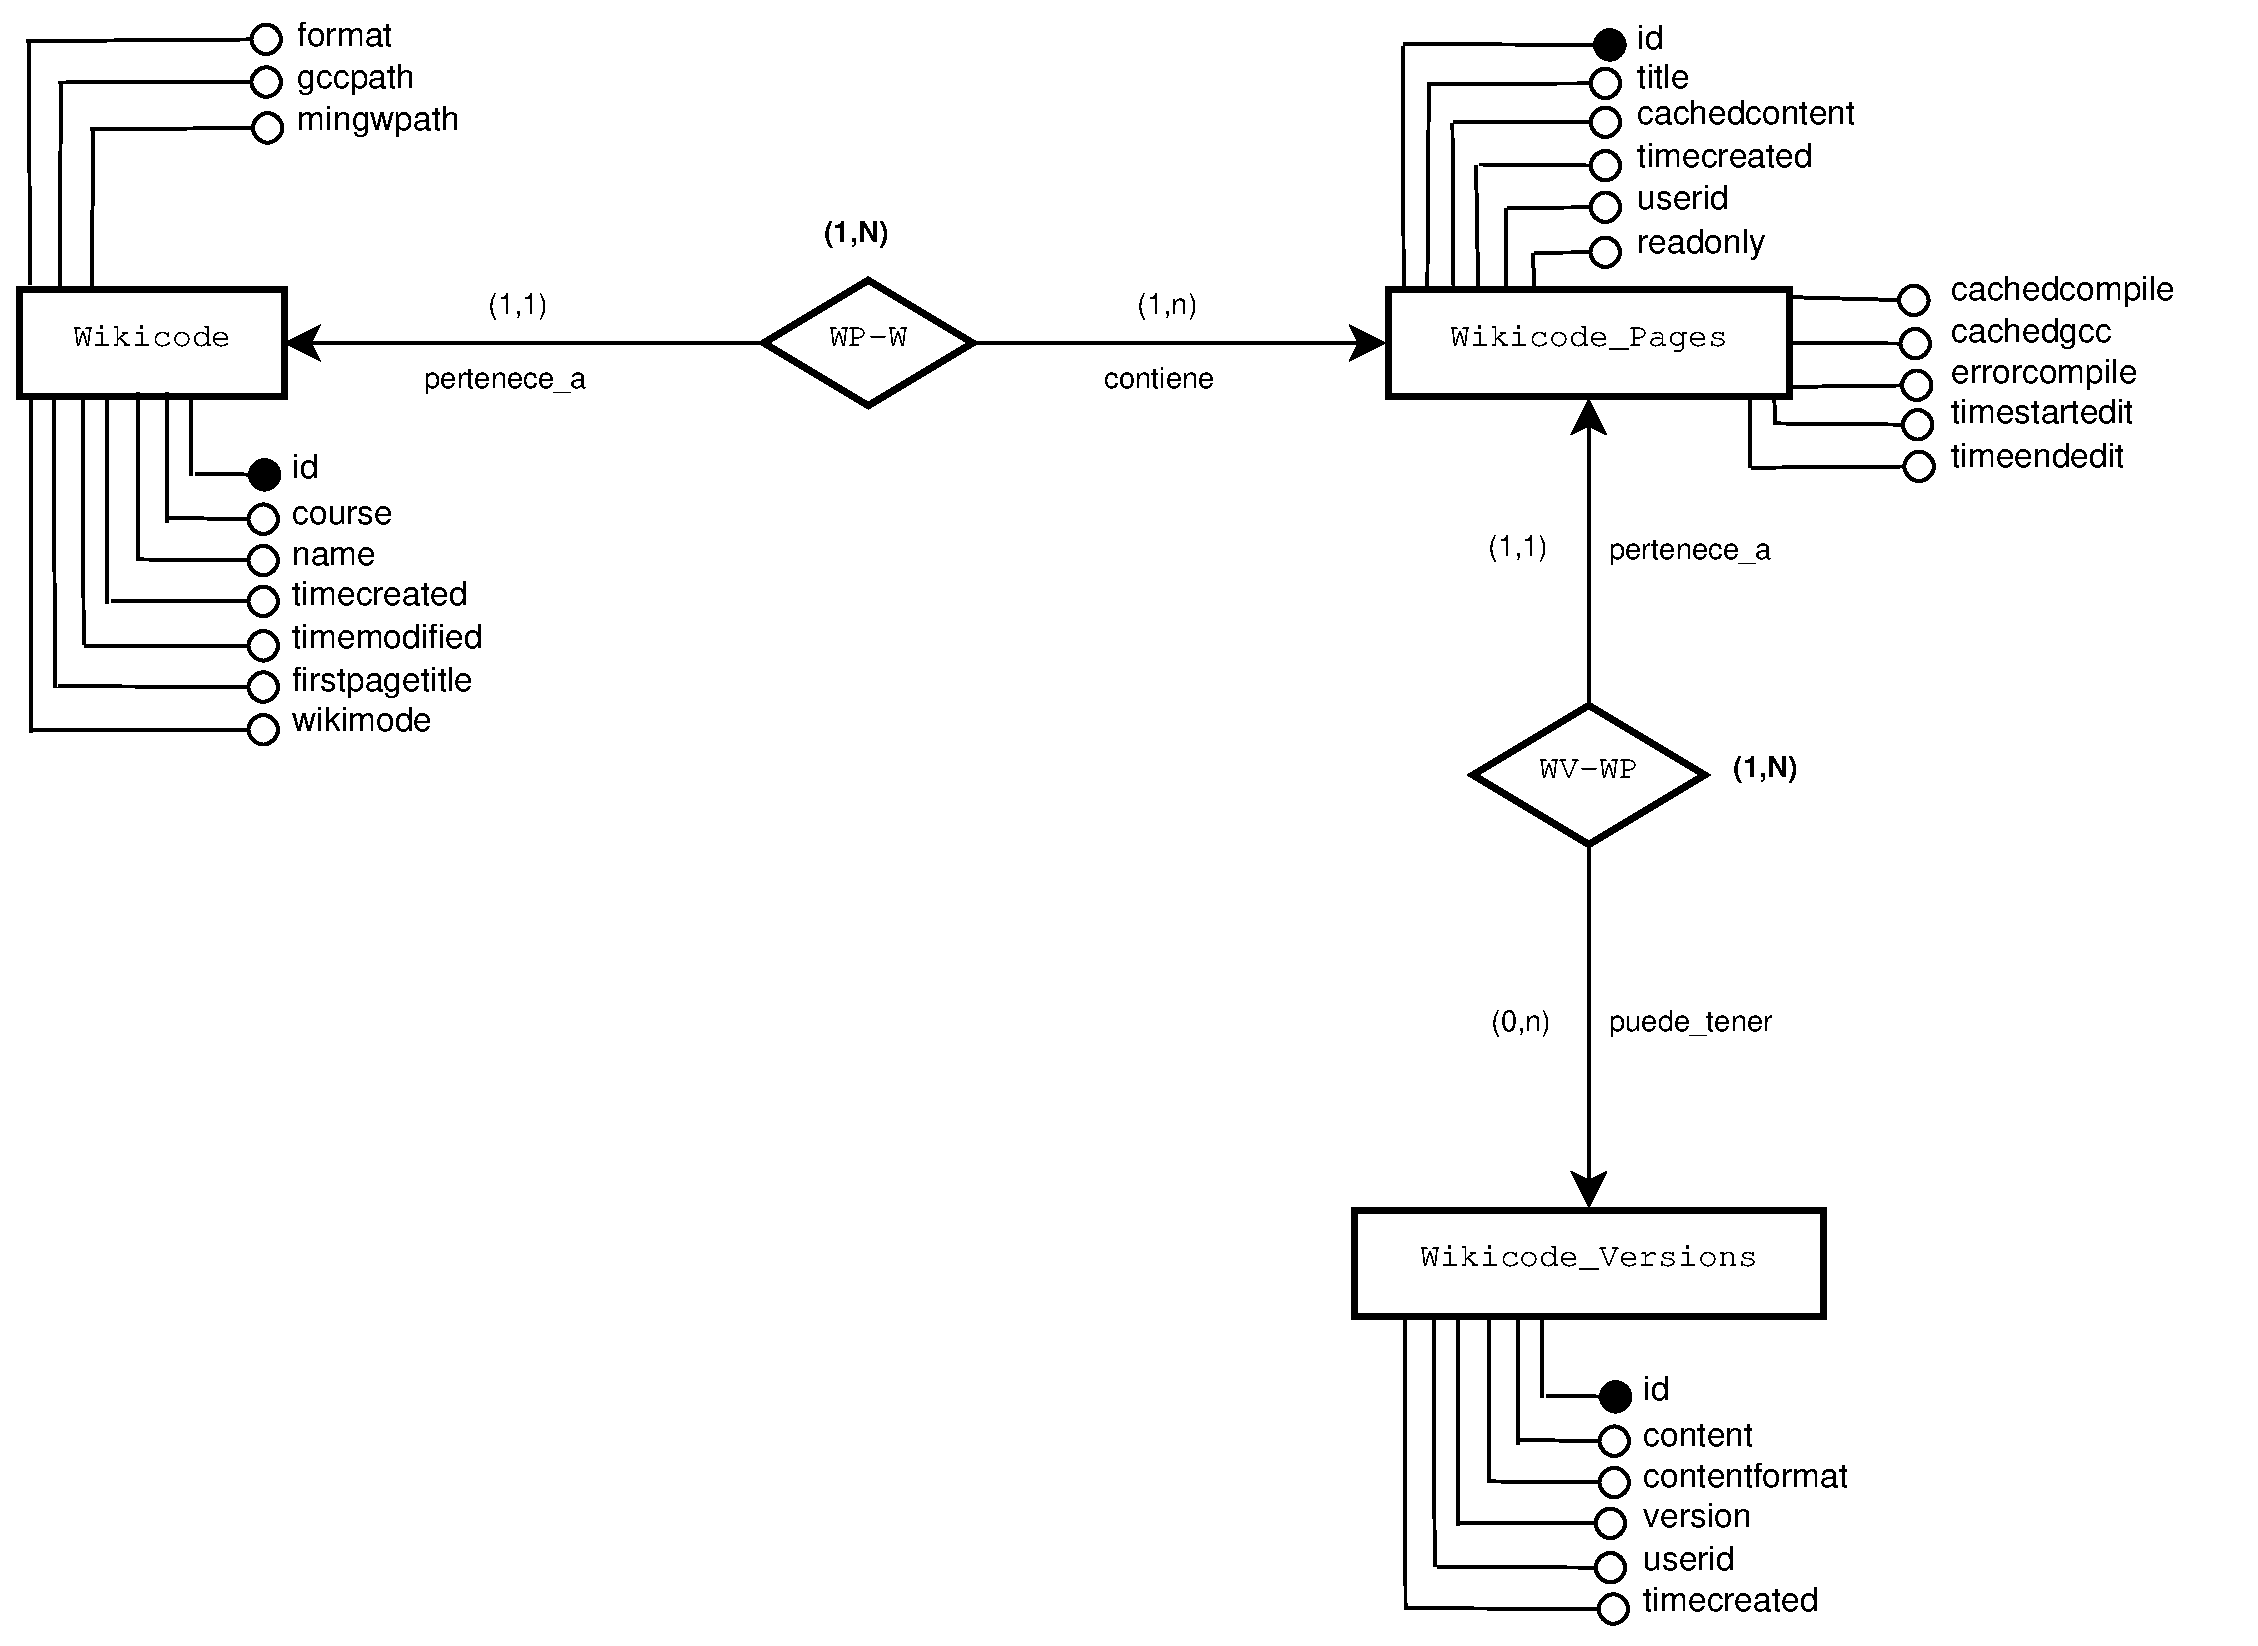
\includegraphics[width=\textwidth]{./img/EER.eps}
	\caption{Esquema EE-R del modelo conceptual del módulo Wikicode}
\end{figure}
	
	También contará con los atributos correspondiente a la parametrización del compilador, donde dividiremos en el que se querrá usar para Windows y el que se querrá usar para entornos Unix.
	
	\item{\textbf{Tipo de entidad}} \emph{wikicode\_pages}: el cual representa al objeto del mundo real \emph{página} que representa \emph{``el código fuente editado de modo colaborativo en lenguaje C''}. Se van a considerar como atributos el título que se haya considerado al crearse así como el contenido del código. También será necesario una serie de información estadística y de información como es saber el identificador del usuario que lo ha creado, el número de visualizaciones que ha tenido ese código y si sólo queremos que sea de lectura.
	
	También es importante contar con la información del compilador, por lo que se almacenará el código que se ha enviado al compilador y la salida que ha producido este al enviarle dicho código como parámetro. Por último también contaremos con la información estadística necesaria para la visualización de los logs: Hora de primera edición, Hora de última edición y Número de errores de compilación.
	
	\item{\textbf{Tipo de entidad}} \emph{wikicode\_versions}: el cual representa el objeto del mundo real \emph{version} que representa \emph{``el código fuente colaborativo en lenguaje C en un momento específico del tiempo''}. Esta información es necesaria para mantener un histórico por lo que únicamente contaremos como atributos el código fuente de dicha versión, el tipo de contenido, el número de versión que se trata, la hora en que fue creada dicha versión y la información referente al usuario que creó esta entrada.
\end{description}

\subsubsection{Análisis de los tipos de interrelación}

Los tipos de entidad antes mencionados se encuentran relacionados de la siguiente forma:

\begin{description}
	\item{\textbf{Tipo de interrelación}} \emph{Wikicode/Wikicode\_Pages} \textbf{W-WP}: el cual relaciona los tipos de entidad \emph{Wikicode} y \emph{Wikicode\_Pages}, la interrelación es del tipo \emph{1:N}, ya que una página pertenece a una única wikicode, por tanto, el tipo de entidad \emph{Wikicode\_Pages} participa con las cardinalidades \emph{(1,1)} en este tipo de interrelación, mientras que en una Wikicode pueden existir muchas páginas debido a la creación de grupos. Se considera que una Wikicode no tiene sentido sin que existan páginas en su interior, por lo que el tipo de entidad \emph{Wikicode} participara en el tipo de interrelación \emph{W-WP} con las cardinalidades \emph{(1,n)} como se puede observar en la figura 4.1.
	
	\item{\textbf{Tipo de interrelación}} \emph{Wikicode\_Pages/Wikicode\_Version} \textbf{WP-WV}: el cual relaciona los tipos de entidad \emph{Wikicode\_Pages} y \emph{Wikicode\_Versions}, la interrelación es del tipo \emph{1:N}, ya que una versión del histórico pertenece a un único código fuente, por tanto, el tipo de entidad \emph{Wikicode\_Versions} participa con las cardinalidades \emph{(1,1)} en este tipo de interrelación, mientras que de un código fuente pueden existir muchas versiones en un histórico. No hay necesidad de que un código fuente tenga almacenada información en su histórico, por lo que el tipo de entidad \emph{Wikicode\_Pages} participara en el tipo de interrelación \emph{WP-WV} con las cardinalidades \emph{(0,n)} como se puede observar en la figura 4.1.
\end{description}

\newpage

\subsection{Modelo Relacional}

Una vez realizado el modelo conceptual se va a construir el modelo relacional del problema considerado.

\subsubsection{Tabla Wikicode}

La tabla \emph{Wikicode} se forma a partir del tipo de entidad \emph{Wikicode}. Esta tabla incluye los atributos \emph{id, course, name, timecreated, timemodified, firstpagetitle, wikimode, format, gccpath} y \emph{mingwpath} que son tomados del tipo de entidad antes mencionado (regla RTECAR-1).

La clave principal de la tabla es el atributo \emph{id}, no considerándose, en este caso, ningún otro atributo que pueda ser utilizado como identificador alternativo, y ninguno de los atributos de esta tabla mantiene referencia alguna con los atributos de las otras tablas. La tabla \emph{Wikicode} queda de la siguiente forma:

\begin{description}
	\item{\textbf{Wikicode}} \emph{(\underline{id}, course, name, timecreated, timemodified, firstpagetitle, wikimode, format, gccpath, mingwpath)}
\end{description}

\subsubsection{Tabla Wikicode\_Pages}

La tabla \emph{Wikicode\_Pages} se forma a partir del tipo de entidad del mismo nombre tomando los atributos de este tipo de entidad (regla RTECAR-1), además de:

\begin{itemize}
	\item El atributo identificador de la tabla \emph{Wikicode} con la cual mantiene una relación uno a muchos (regla RTECAR-3.1).
\end{itemize}

La clave principal de la tabla es el atributo \emph{id}, no considerándose, en este caso, ningún otro atributo que pueda ser utilizado como identificador alternativo.

\begin{description}
	\item{\textbf{Wikicode\_Pages}} \emph{(\underline{id}, title, cachedcontent, timecreated, userid, readonly, cachedcompile, cachedgcc, errorcompile, timestartedit, timeendedit, \textbf{subwikiid})}
\end{description}

\subsubsection{Tabla Wikicode\_Versions}

La tabla \emph{Wikicode\_Versions} se forma a partir del tipo de entidad del mismo nombre tomando los atributos de este tipo de entidad (regla RTECAR-1), además de:

\begin{itemize}
	\item El atributo identificador de la tabla \emph{Wikicode\_Pages} con la cual mantiene una relación uno a muchos (regla RTECAR-3.1).
\end{itemize}

La clave principal de la tabla es el atributo \emph{id}, no considerándose, en este caso, ningún otro atributo que pueda ser utilizado como identificador alternativo.

\begin{description}
	\item{\textbf{Wikicode\_Pages}} \emph{(\underline{id}, content, contentformat, version, timecreated, \textbf{pageid})}
\end{description}

\subsection{Normalización del modelo}

\begin{description}
	\item{\textbf{Table} \emph{Wikicode}}: esta tabla se encuentra en FNBC, pues todos los atributos son atómicos (FN1) y las dependencias funcionales son completas.
\end{description}

\begin{description}
	\item{\textbf{Table} \emph{Wikicode\_Pages}}: al igual que en el caso anterior, esta tabla se encuentra en FNBC.
\end{description}

\begin{description}
	\item{\textbf{Table} \emph{Wikicode\_Versions}}: por el mismo razonamiento esta tabla se encuentra en FNBC.
\end{description}

\begin{figure}[h]
	\centering
	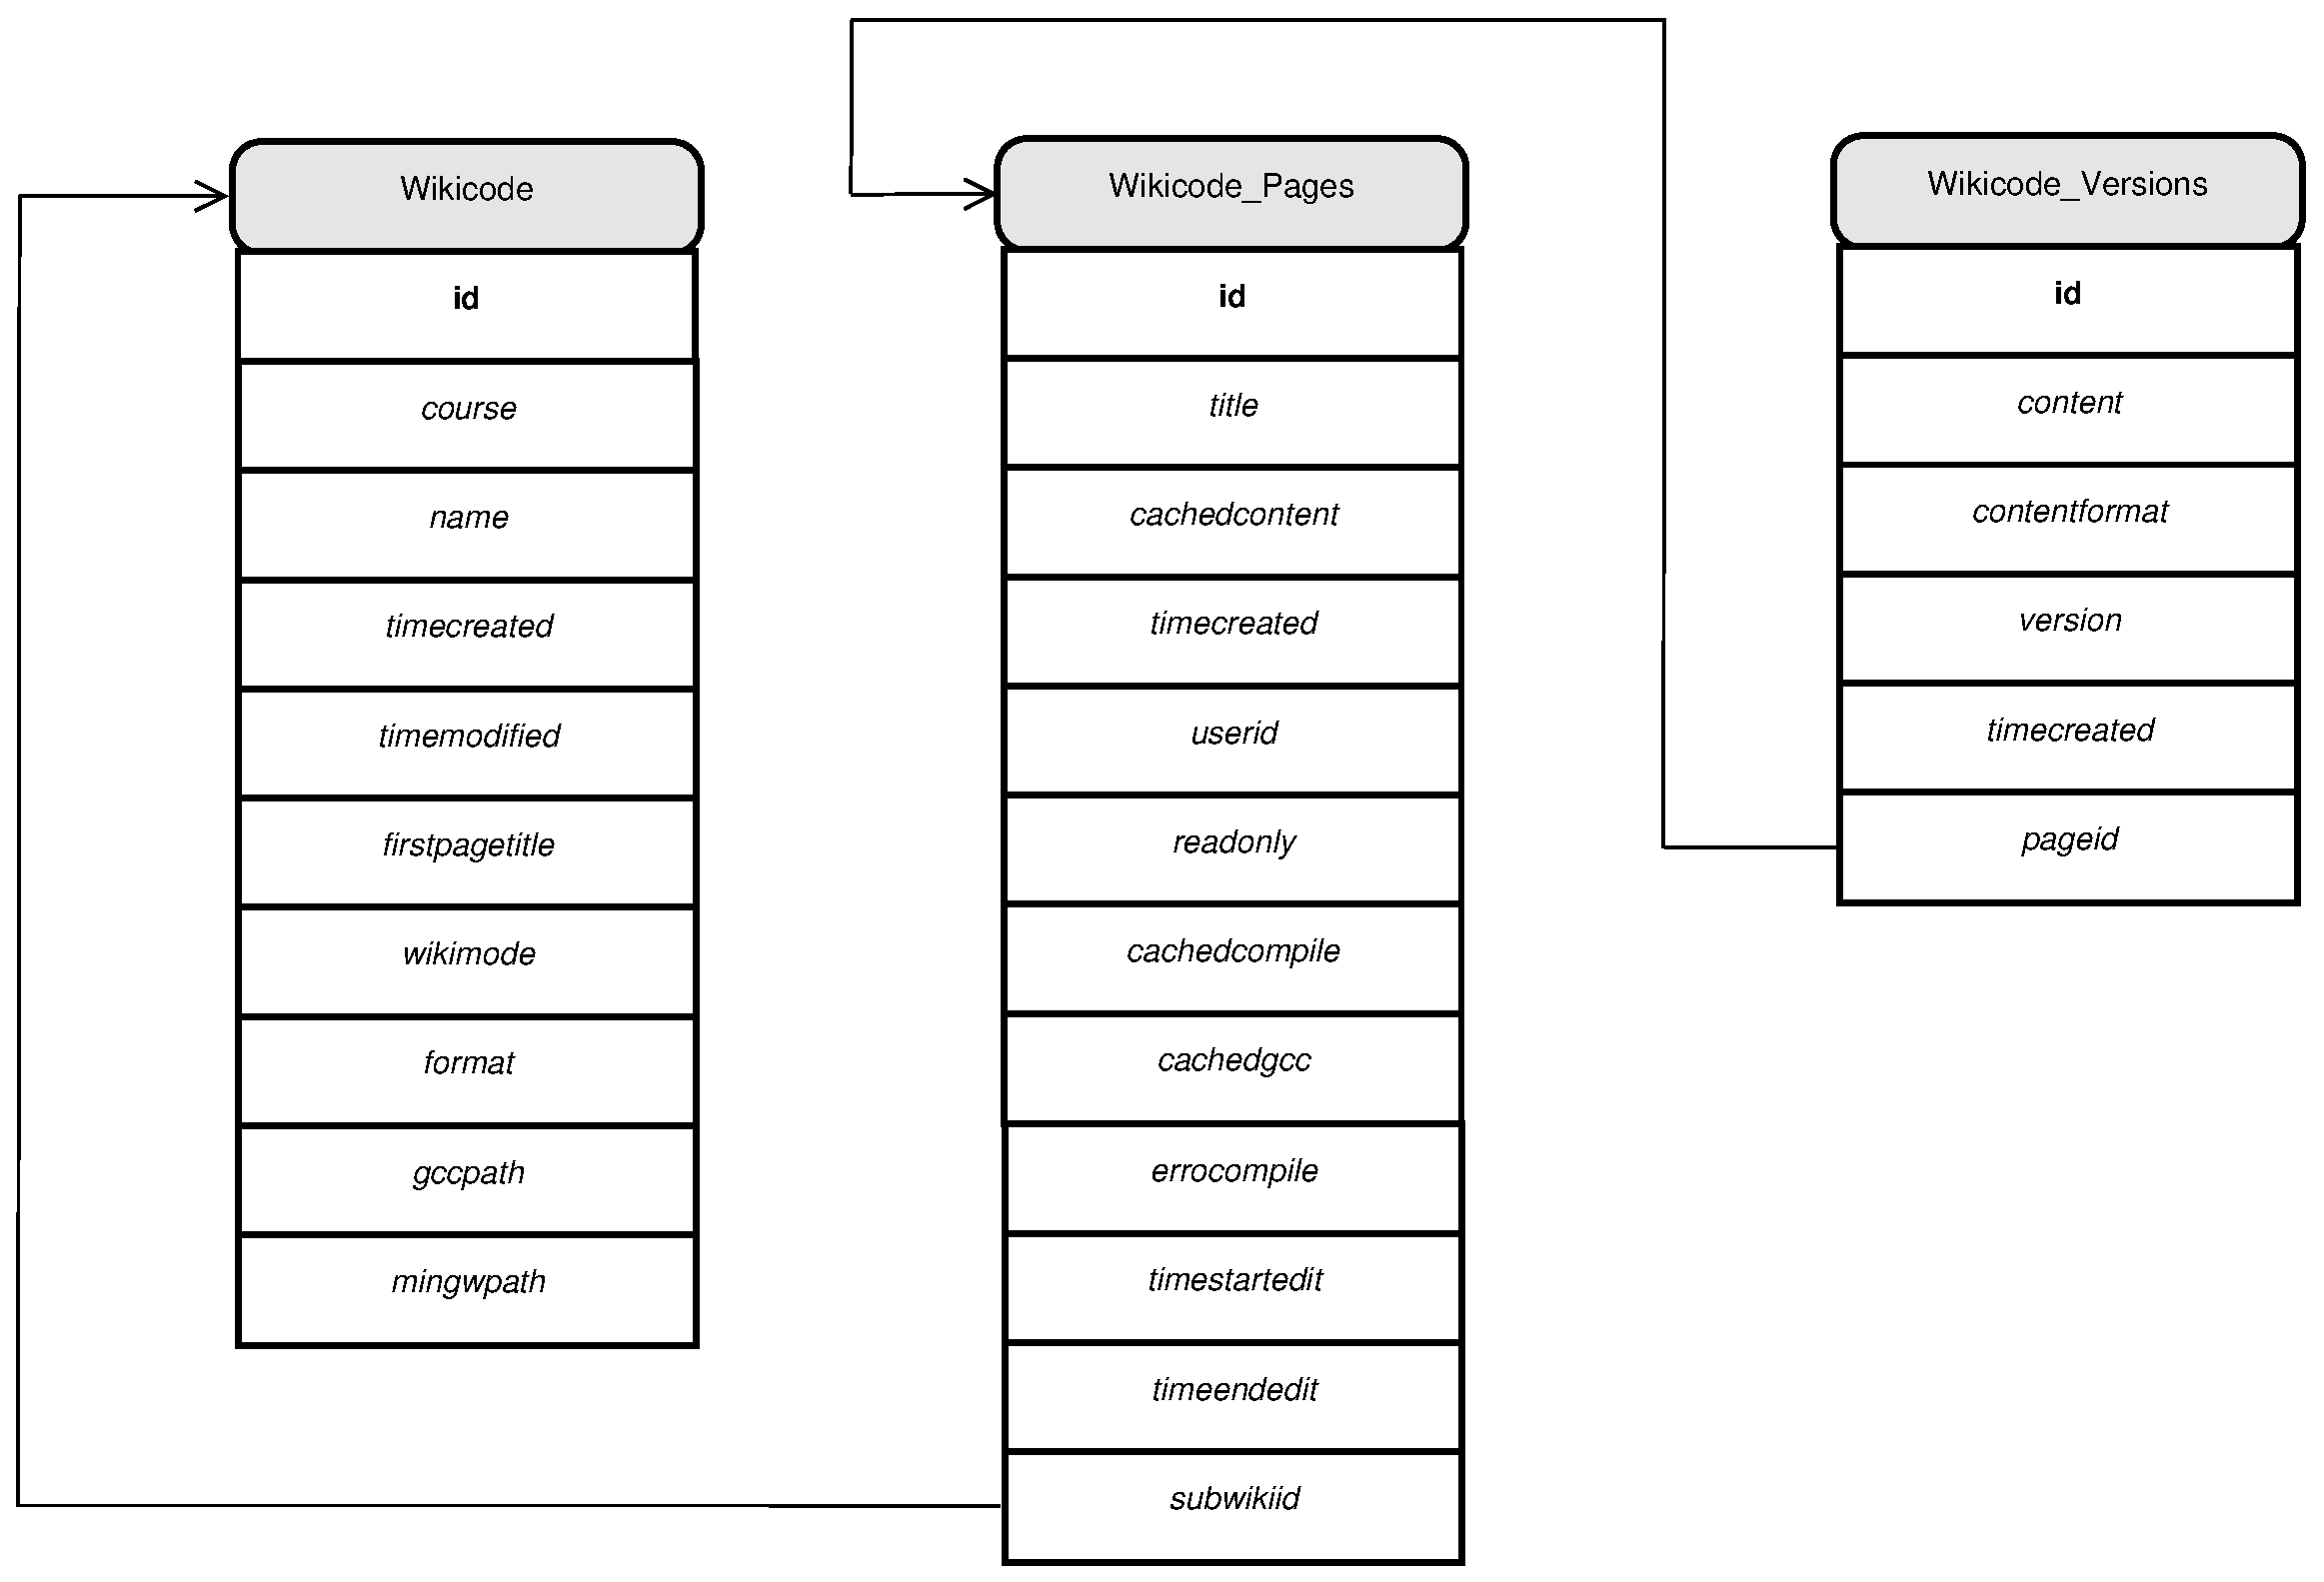
\includegraphics[width=\textwidth]{./img/ERelacional.eps}
	\caption{Diagrama relacional para el módulo Wikicode}
\end{figure}

\section{Descripción del resultado final del interfaz}

En este apartado se describirá cómo interactúa el sistema con el usuario, definiendo la estructura y comportamiento del interfaz. Aunque el diseño de esta interfaz no es uno de los objetivos primordiales del proyecto, se ha intentado realizar un diseño de manera que se facilite el manejo del sistema al usuario aprovechando las características del entorno Moodle. Además, para la parte en que el usuario va a editar el código fuente, se ha simulado un editor con características similares a cualquier otro editor de código que se pueda encontrar.

\subsection{Descripción del interfaz}

En cuanto a la estructura general del interfaz del módulo desarrollado, hay que tener en cuenta que nuestro proyecto se ha centrado en la realización de un módulo que pueda ser utilizado en Moodle.

De esta manera, el diseño de los módulos por defecto de Moodle se ha tomado como base para el desarrollo del nuevo bloque. Este hecho permite conseguir homogeneidad del sistema de manera que todos los bloques y elementos se encuentren en consonancia.

Por tanto, nos limitaremos a hablar del diseño realizado para el bloque en cuestión sin especificar características especiales de Moodle.

\newpage
\subsection{Descripción de las pantallas del interfaz}

\subsubsection{Pantalla principal}

Al tratarse de un módulo la creación de una Wikicode y su posterior selección será igual a la otro cualquiera (Foro, Wiki, Chat, Cuestionario, etc.). En la siguiente figura se muestra como se añadiría una nueva Wikicode a un curso ya creado:

\begin{figure}[h]
	\centering
	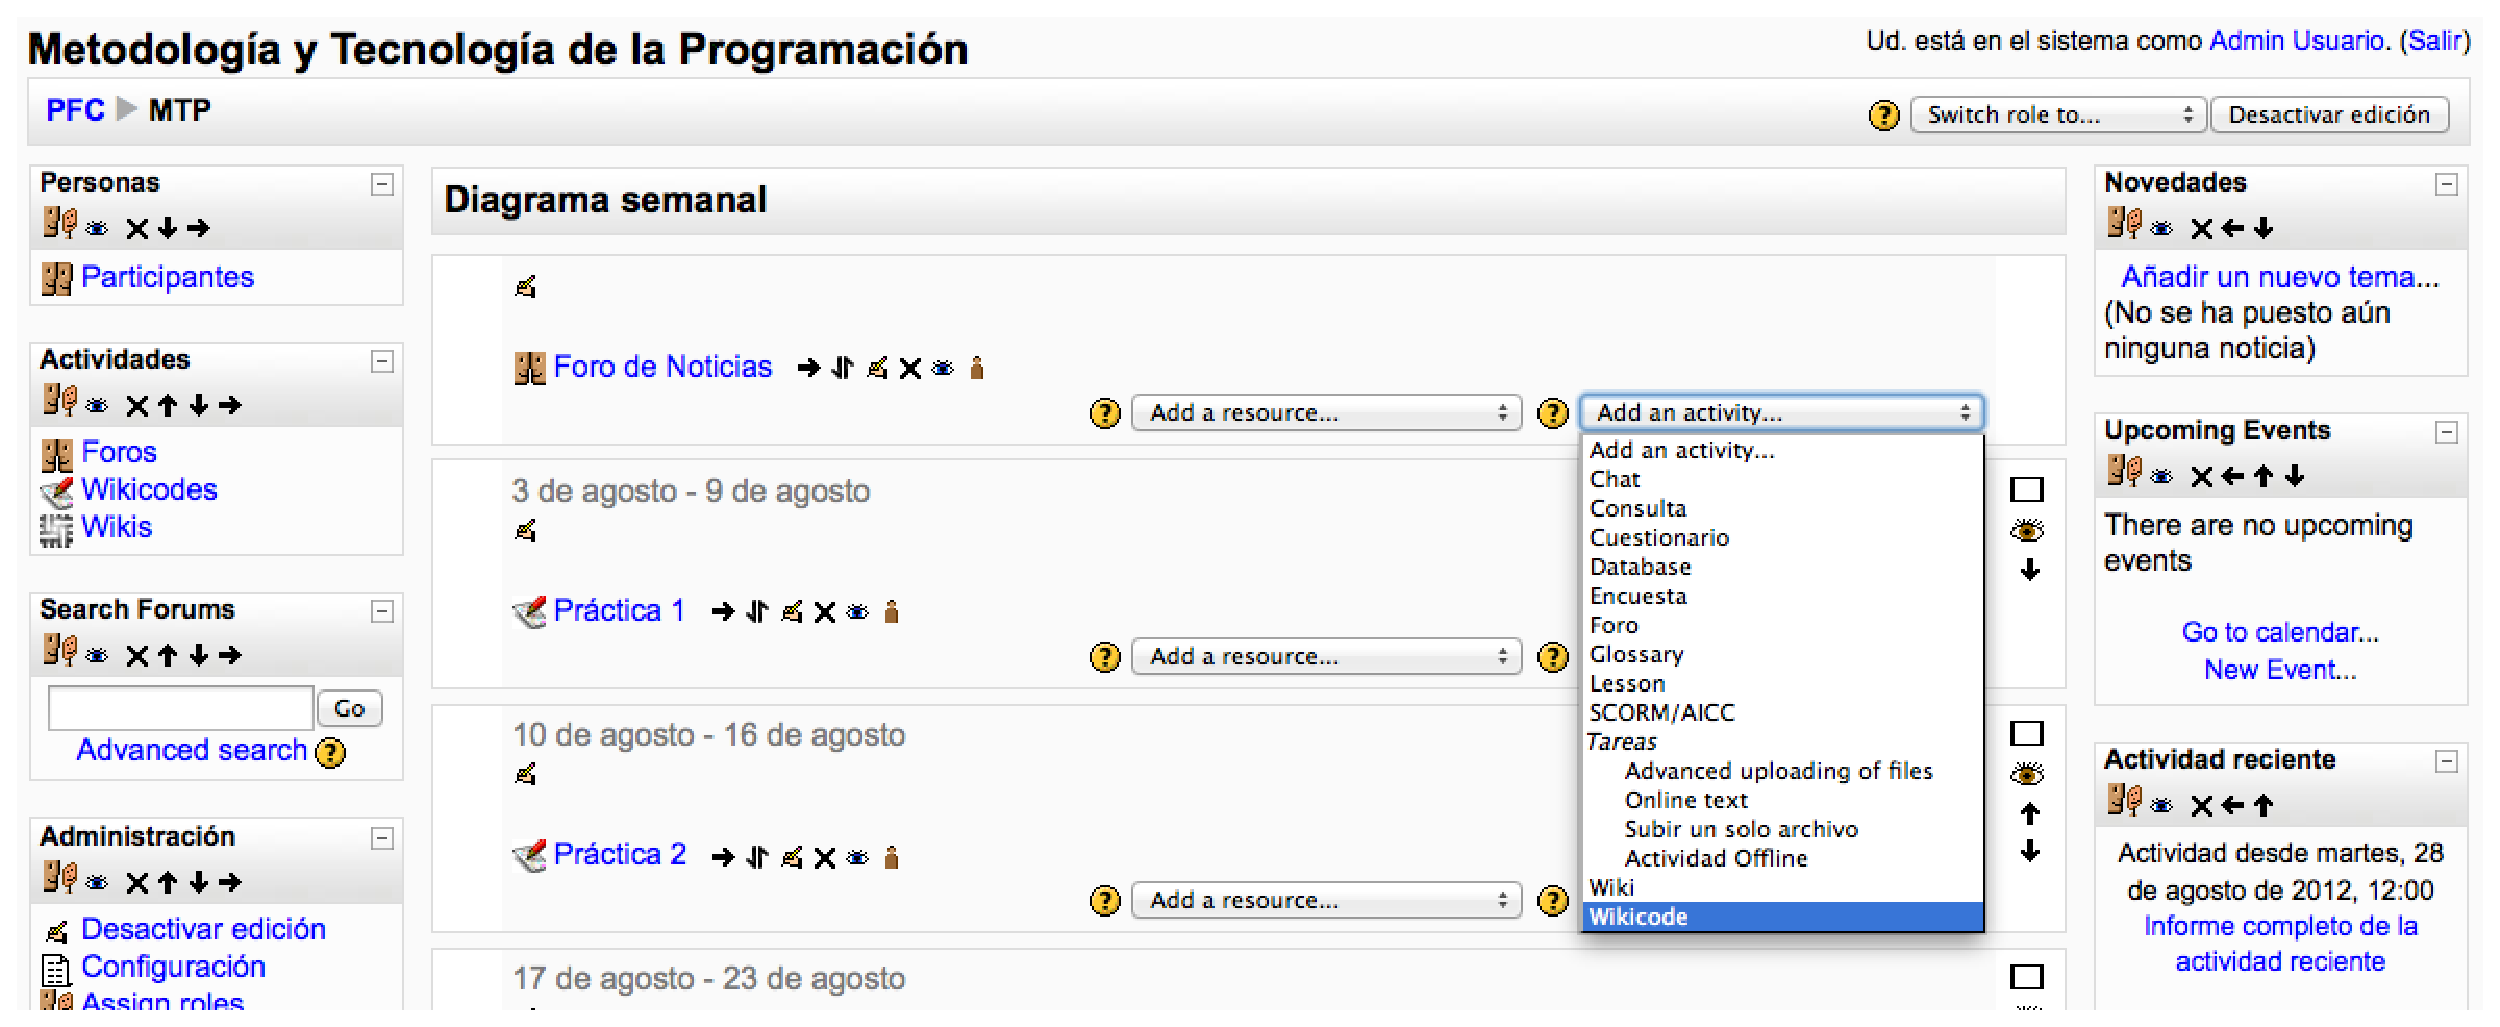
\includegraphics[width=\textwidth]{./img/c4main.eps}
	\caption{Pantalla principal de un curso Moodle añadiendo una Wikicode}
\end{figure}

\subsubsection{Pantalla configuración y parametrización}

Cuando se accede a la opción de crear una nueva Wikicode se accede a la pantalla de configuración del módulo. Este formulario contendrá todas las variables para la creación del entorno colaborativo deseado. En concreto las variables a tener en cuenta será la elección del nombre y la descripción del mismo, la posibilidad de agrupamiento con respecto a una Wikicode (eligiendo de una lista) y la parametrización del compilador que desea usarse.

Para ayudar al tutor, se ha optado por una ayuda automática a la hora de parametrizar los compiladores, tomando siempre por defecto el valor que haya sido usado un mayor número de veces con anterioridad. Si nunca se ha usado ninguno por defecto aparecerá el nombre del compilador recomendado.

\newpage

En la siguiente figura se muestra la pantalla de configuración que se presenta cuando se decide crear una nueva Wikicode:

\begin{figure}[h]
	\centering
	\includegraphics[width=0.68\textwidth]{./img/c4param.eps}
	\caption{Pantalla de configuración y parametrización Wikicode}
\end{figure}

Además, a partir de la versión 2 de Moodle se ha actualizado el módulo para que cada opción traiga consigo una ayuda que nos explique la funcionalidad de cada variable.

\begin{figure}[h]
	\centering
	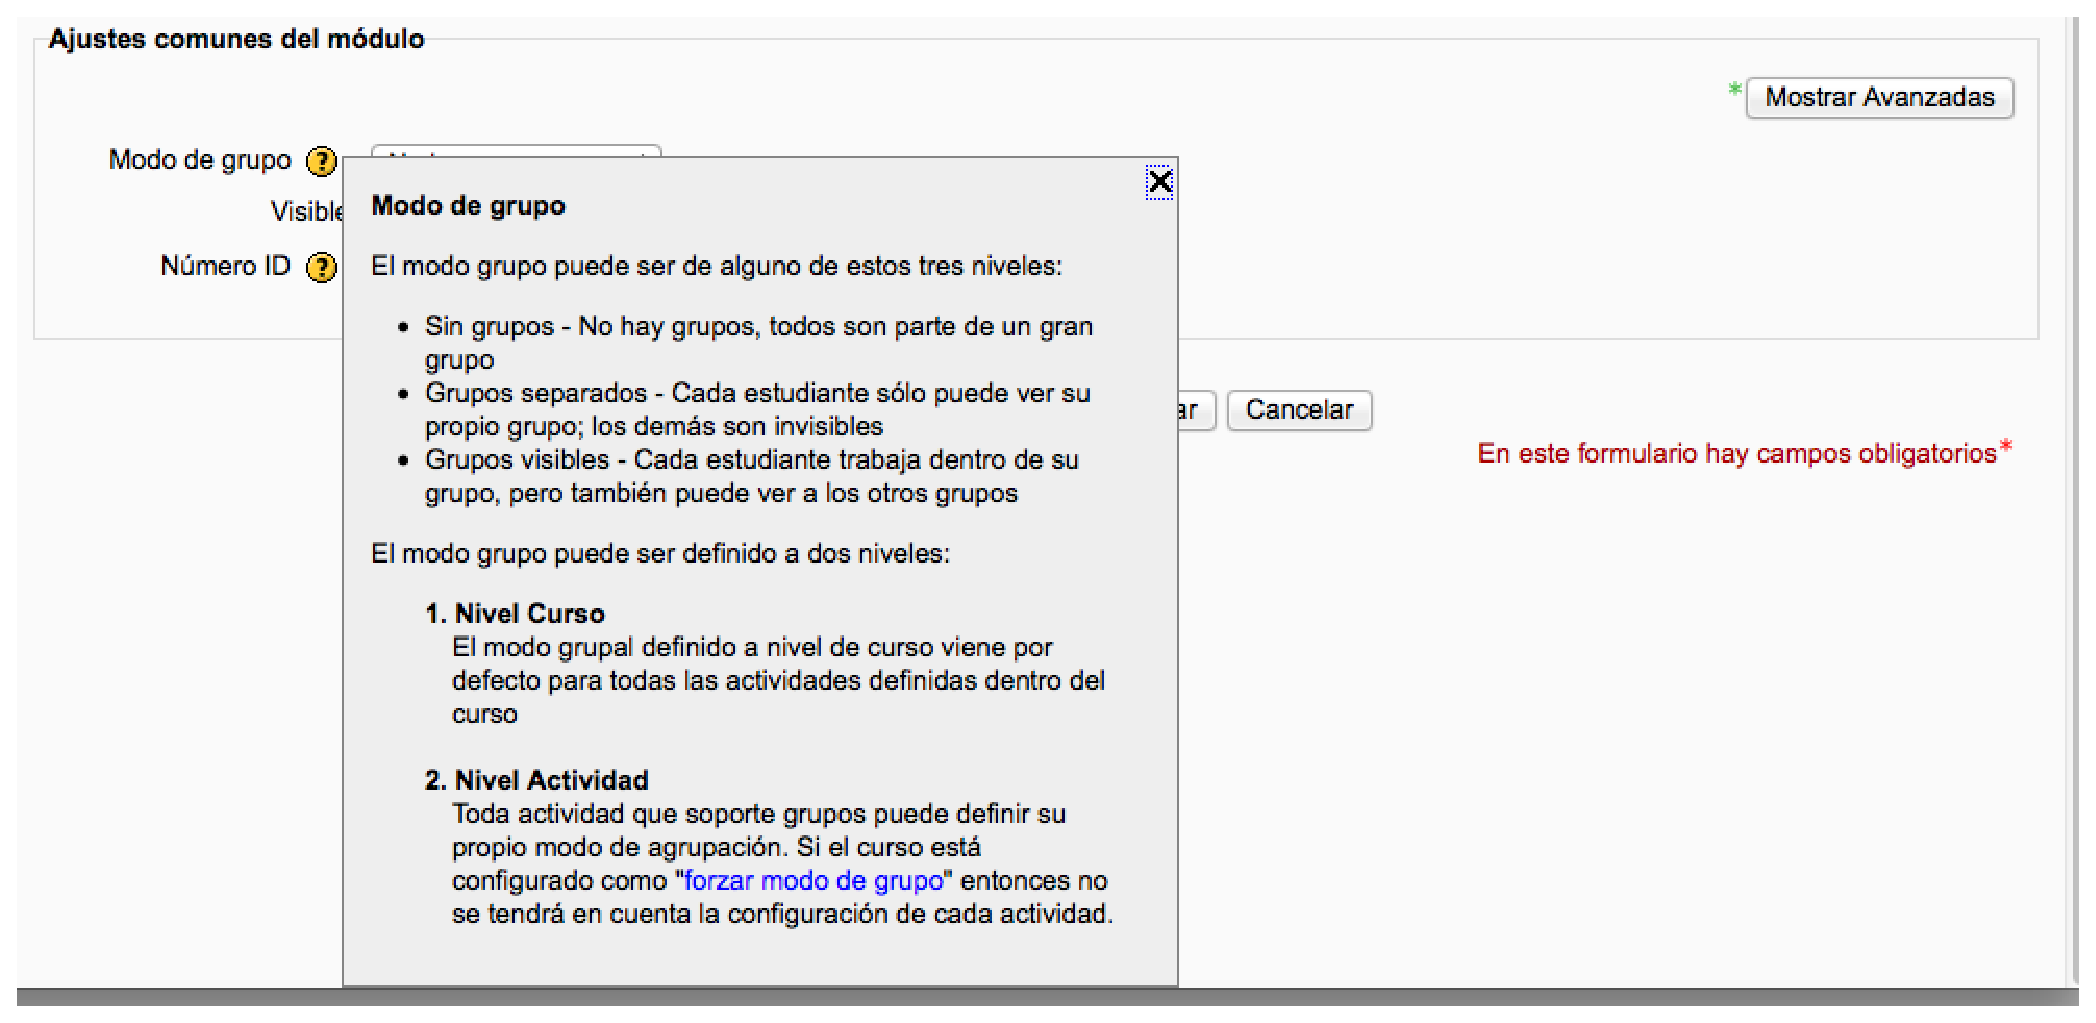
\includegraphics[width=0.7\textwidth]{./img/c4paramhelp.eps}
	\caption{Pantalla de ayuda a la configuración Wikicode}
\end{figure}

\newpage

\subsubsection{Pantalla cabecera superior}

Como su propio nombre indica, no se trata de un interfaz completo en sí, sino de la parte superior que compartirán todas las páginas definidas dentro del módulo Wikicode. Esta cabecera, compartida, la podemos dividir en las siguientes partes.

\begin{itemize}
	\item \textbf{Nombre del curso:} Etiqueta informativa sobre el nombre del curso al que pertenece la Wikicode.
	\item \textbf{Listado de navegación:} Menú de tipo lista que nos permite acceder al resto de contenidos del curso.
	\item \textbf{Árbol de directorio:} Nos representa un listado de donde nos encontramos ahora mismo, situándonos en el curso, la categoría y el nombre que hayamos dado al módulo. Será navegable y permite enlazar rápidamente a cada una de ellas.
	\item \textbf{Actualización:} Si el usuario tiene permisos de administración le aparecerá este botón, el cual permite acceder a la parametrización de la Wikicode que nos encontremos y modificar sus opciones.
	\item \textbf{Menú de contenido:} Menú de navegación que nos permite desplazarnos rápidamente por las opciones de nuestro editor de desarrollo. Se marcará la opción sobre la que nos encontremos en el momento.
\end{itemize}

En la siguiente figura se muestra la cabecera que se presentará en todas las opciones del módulo Wikicode:

\begin{figure}[h]
	\centering
	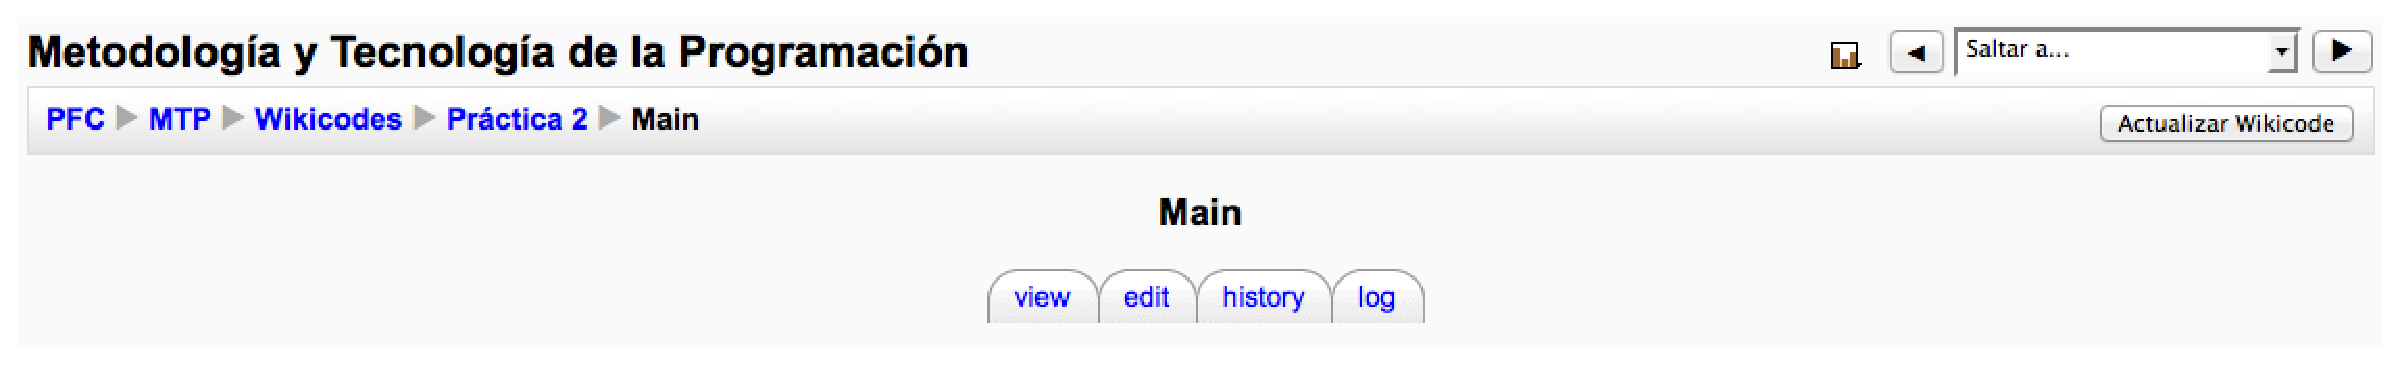
\includegraphics[width=\textwidth]{./img/c4menu.eps}
	\caption{Pantalla cabecera Wikicode}
\end{figure}

\newpage

\subsubsection{Pantalla visualización}

Se trata de la pantalla donde el usuario puede consultar, en formato texto plano, el código fuente de la Wikicode. La pantalla comparte el menú superior con el resto de opciones y simplemente nos mostrará esta información.

Sin embargo, para mayor utilidad de la misma, si el tutor ha decidido crear la Wikicode de modo grupal le aparecerá un menú donde podrá seleccionar el grupo que desee visualizar. Esta opción también será activa para los alumnos en caso de que el tutor así lo marcara.

En la siguiente figura se muestra el formulario de visualización con la opción de selección de grupos activada:

\begin{figure}[h]
	\centering
	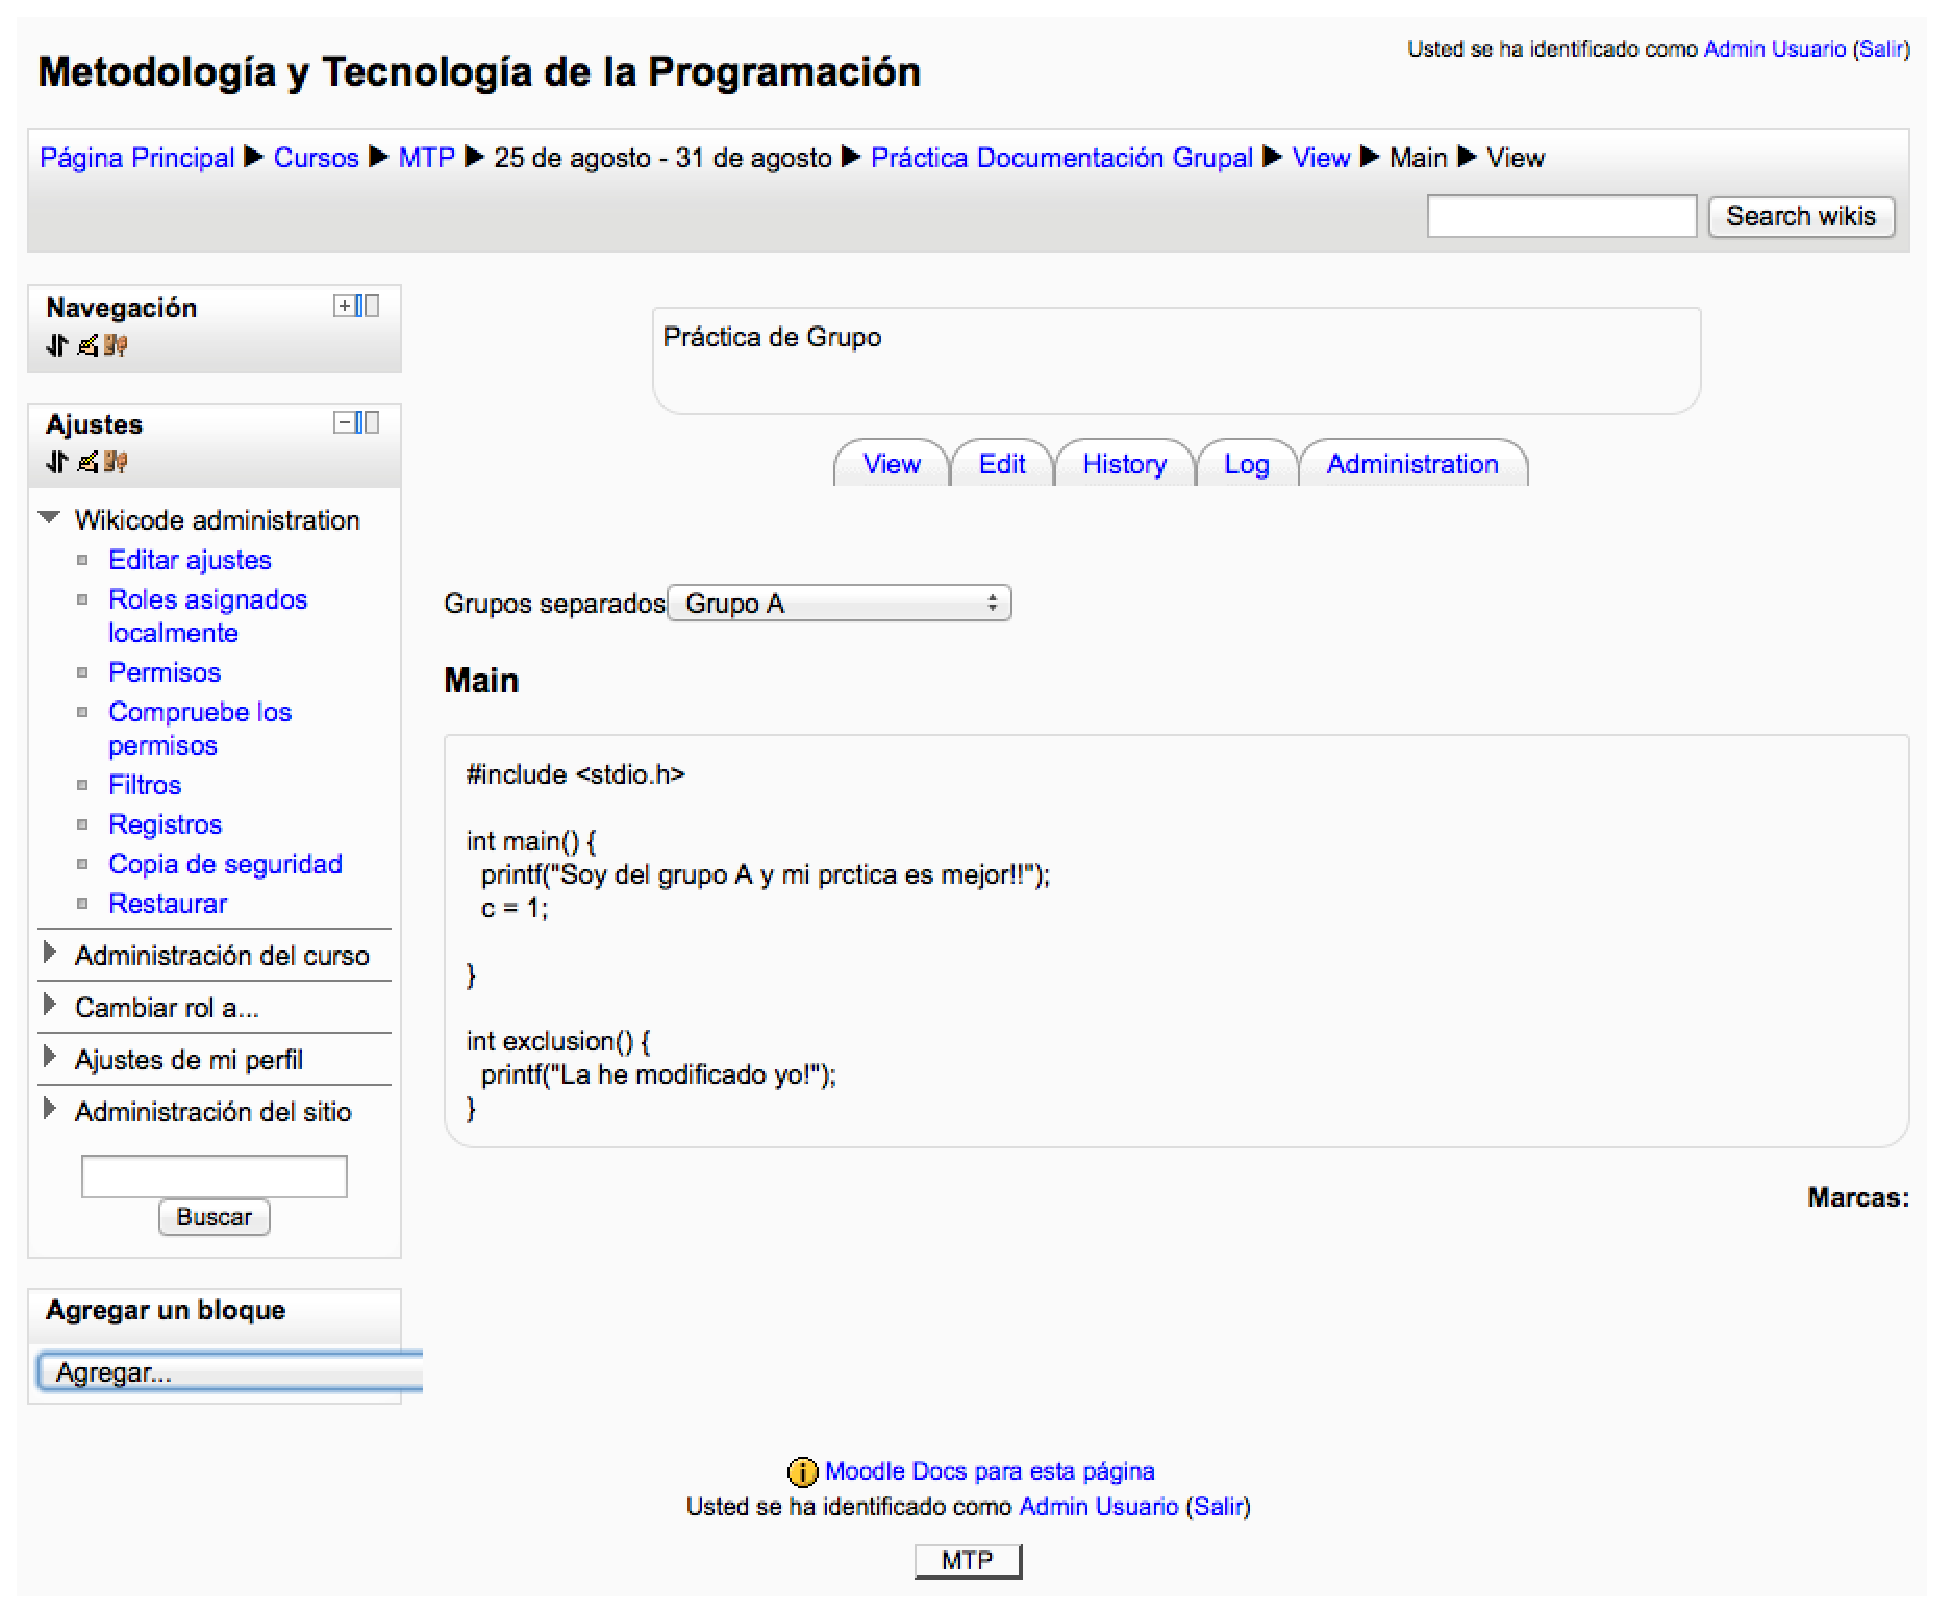
\includegraphics[width=\textwidth]{./img/c4view.eps}
	\caption{Pantalla visualización Wikicode}
\end{figure}

\newpage

\subsubsection{Pantalla edición}

Se trata de la pantalla clave del entorno de desarrollo, en la cual podremos editar el código fuente, comunicarnos con el resto de usuarios y compilar nuestro código para ver que errores puede contener.

\begin{figure}[h]
	\begin{center}
	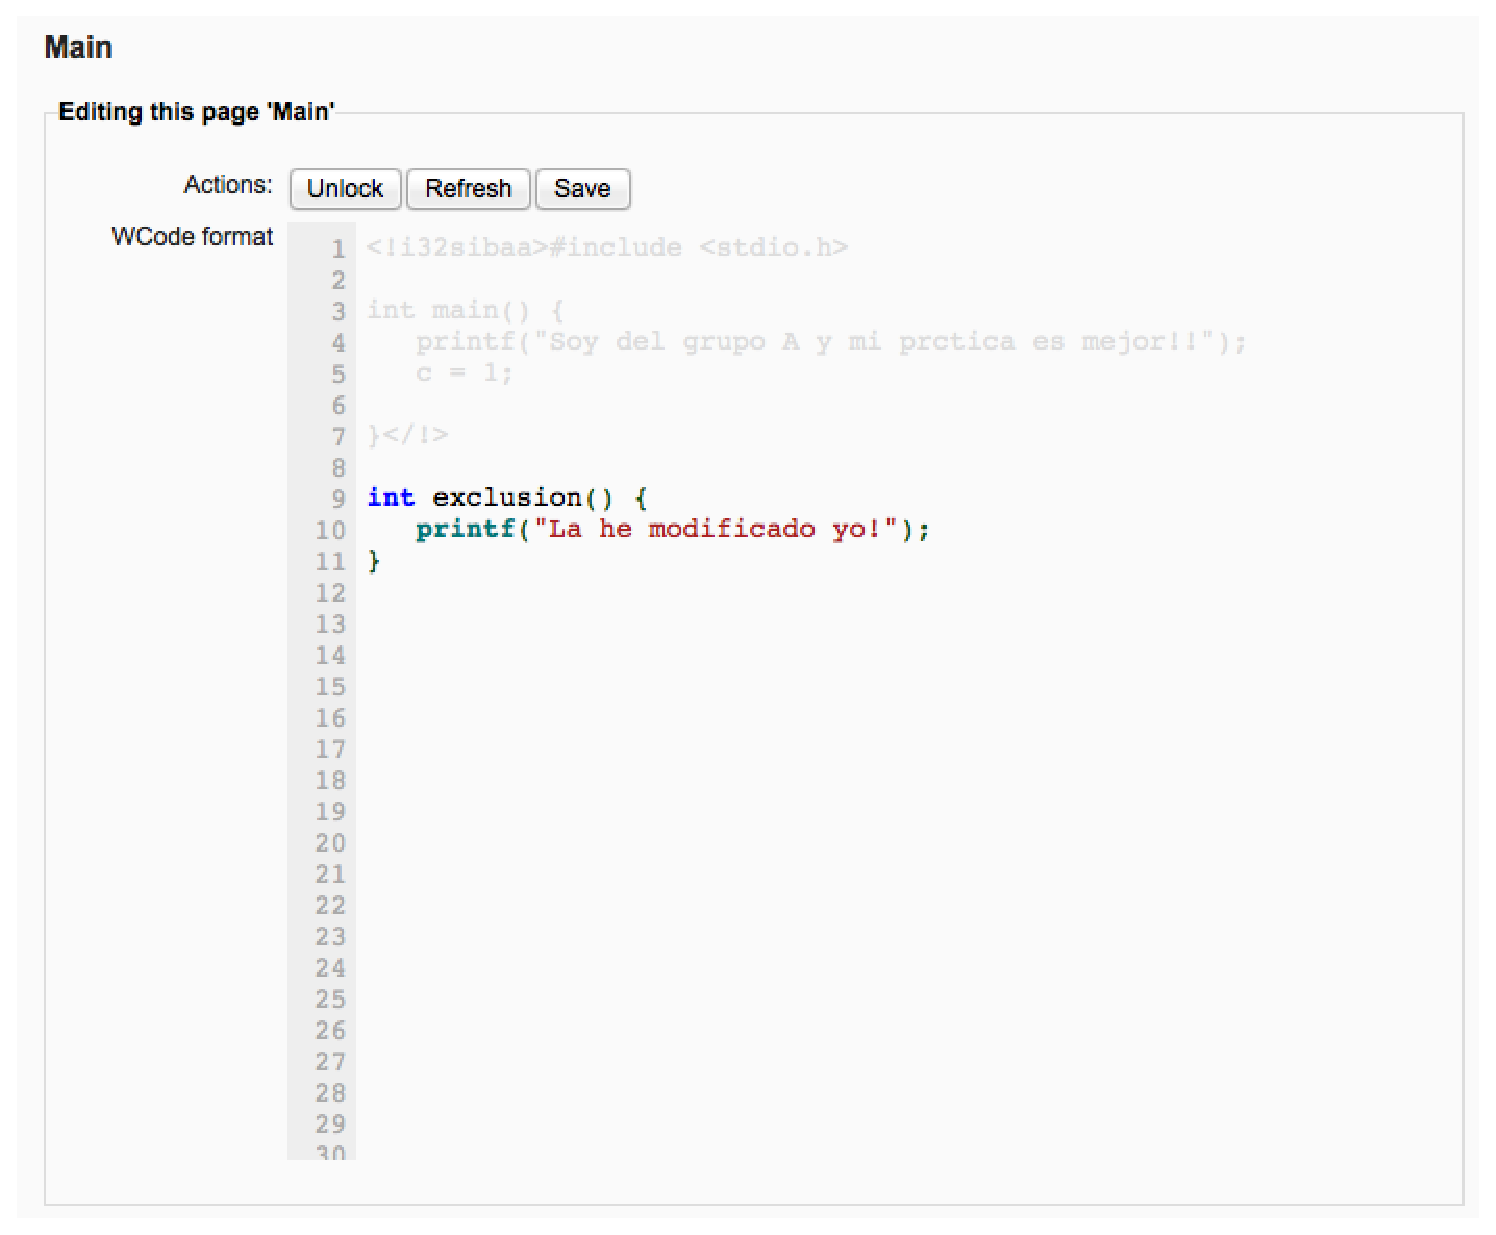
\includegraphics[width=\textwidth]{./img/c4edit.eps}
	\caption{Pantalla editor Wikicode.}
	\end{center}
\end{figure}

El editor de código se irá actualizando a medida que el usuario va escribiendo. Del mismo modo, si intentamos escribir en una parte del código bloqueada el editor nos impedirá esa acción. Las partes bloqueadas por otros usuarios están claramente diferenciadas en otro color y a su vez se nos informa que usuario es el dueño de dicha parte.

Para comodidad del usuario final, se da formato y color al código conforme a los estándares en C siguiendo este estilo:

\begin{description}
	\item[Comentarios]: Color marrón [\#BB9977]
	\item[Palabra clave]: Color azul y tipografía en negrita.
	\item[Cadena]: Color burdeos [\#AA2222]
	\item[Números]: Color verde claro [\#3A3]
	\item[Funciones]: Color turquesa [\#077] y tipografía en negrita.
	\item[Definición]: Color verde oscuro.
	\item[Bloqueo]: Color gris claro.
\end{description}

Los botones de la parte superior de este apartado actúan del siguiente modo:

\begin{description}
	\item[Unlock]: Nos abre una ventana de estilo pop-up que nos permite desbloquear las funciones que tengamos bloqueadas del código. Podemos elegir entre una, varias o todas.

\begin{figure}[h]
	\begin{center}
	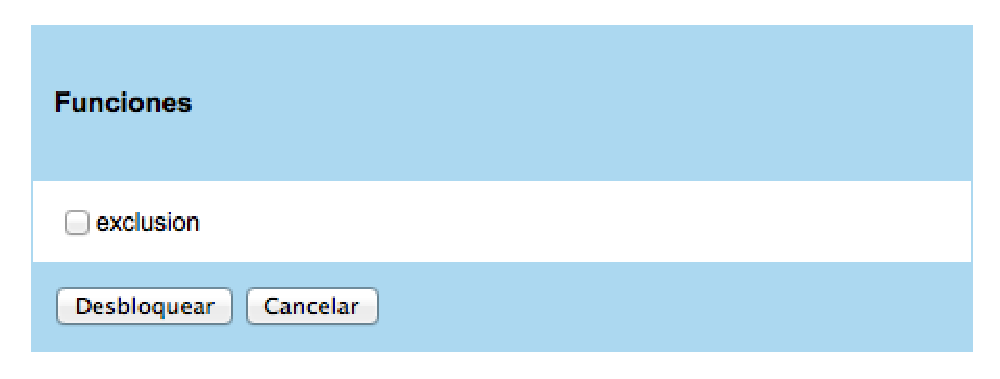
\includegraphics[width=0.5\textwidth]{./img/c4unlock.eps}
	\caption{Pantalla desbloqueo Wikicode.}
	\end{center}
\end{figure}
	
	\item[Refresh]: Actualiza el código fuente. La actualización es semi-automática, pero si se requiere se puede efectuar esta operación manualmente.
	\item[Save]: Guarda una copia del código fuente en el histórico y desbloquea todas las funciones.
\end{description}

Para comunicarnos con otros usuarios se ha creado un chat, el cual se dividirá en dos partes. La superior mostrará los mensajes que han sido enviados con anterioridad, informándonos del usuario y la hora a la que se envió este mensaje. En la inferior habrá un campo de texto y un botón de envío, los cuales servirán para añadir nueva información al chat.

El diseño de este elemento del formulario se puede contemplar en la siguiente figura:

\begin{figure}[h]
	\begin{center}
	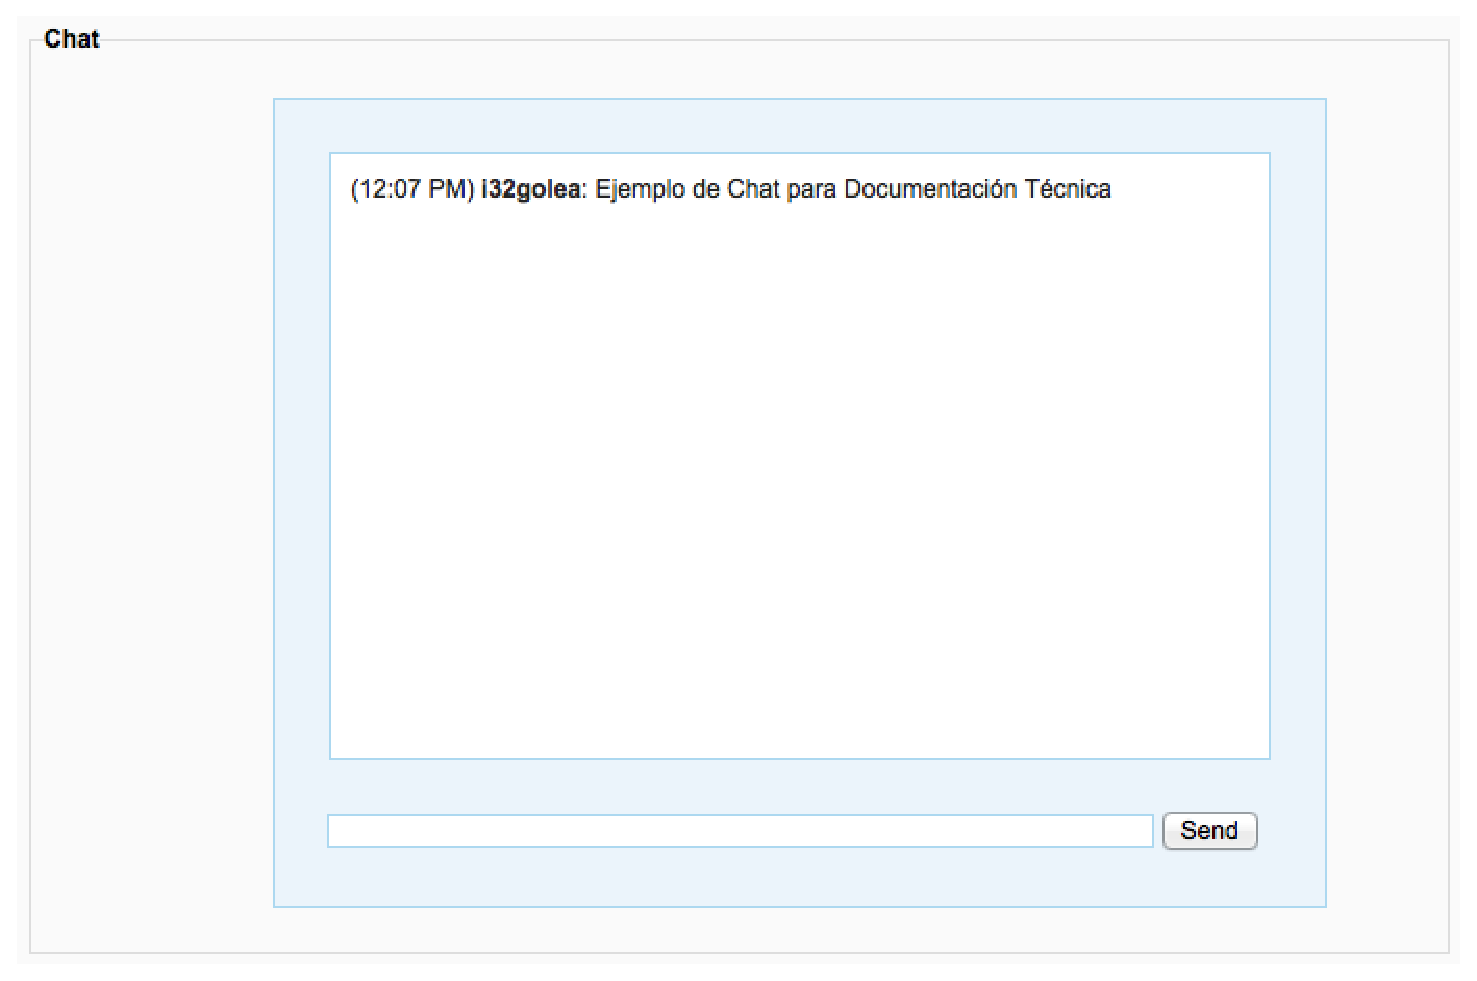
\includegraphics[width=0.65\textwidth]{./img/c4chat.eps}
	\caption{Pantalla chat Wikicode.}
	\end{center}
\end{figure}

Como última parte de este formulario vamos a diseñar la parte dedicada a la compilación, la cual estará dividida en dos partes:

\begin{itemize}
	\item Mensaje: Es el resultado de nuestra compilación, en la que se informará con un mensaje si se ha podido compilar de modo correcto y se nos informará de los errores en caso de que esta premisa no se cumpla. En ella se nos informará del error cometido y se nos proporcionará una pequeña ayuda para solucionarlo.
	\item Botones: Se tratarán de dos botones que nos permitirán dos acciones parejas. En la primera se llamará al compilador para obtener la información sobre nuestro código fuente. La segunda es una ampliación de la primera, la cual llamará al compilador y, si todo es correcto, nos permitirá descargar un ejecutable para ejecutarlo en el equipo cliente.
\end{itemize}

El diseño de este elemento se encuentra en la siguiente figura:

\begin{figure}[h]
	\begin{center}
	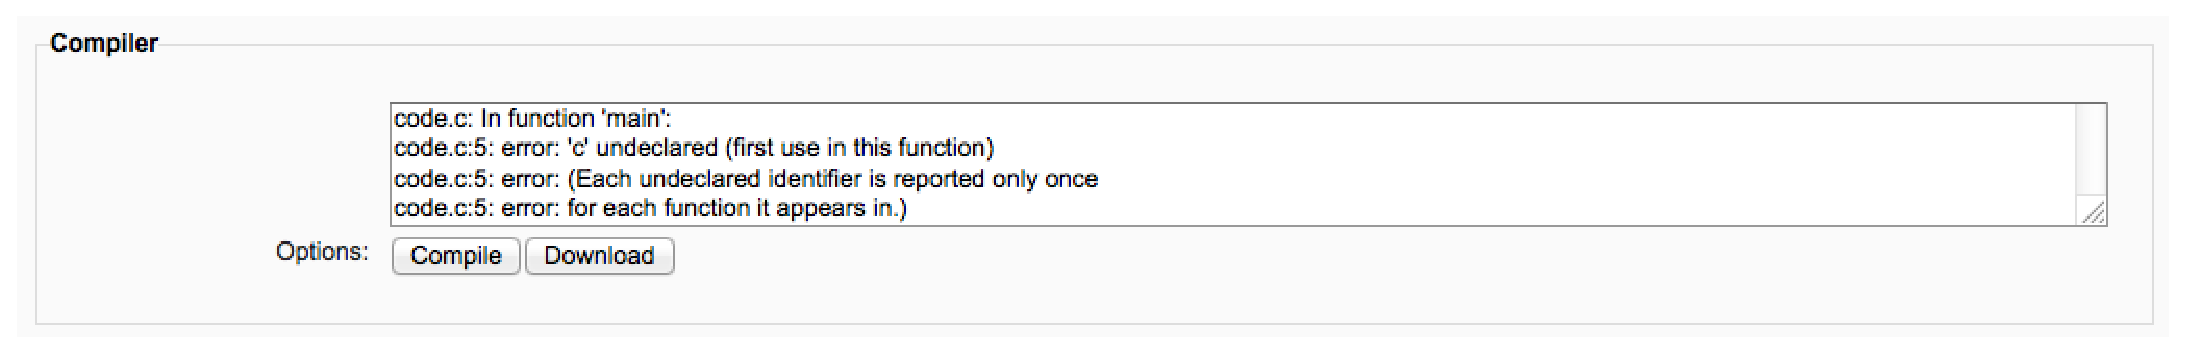
\includegraphics[width=\textwidth]{./img/c4compile.eps}
	\caption{Pantalla compilación Wikicode.}
	\end{center}
\end{figure}

\newpage

\subsubsection{Pantalla histórico}

Como su propio nombre indica, se trata del interfaz que vamos a utilizar para consultar las versiones anteriores de un código fuente. Se proporcionará una lista de versiones y se creará una tabla informando de quién creó dicha versión y cuando la creó.

\begin{figure}[h]
	\begin{center}
	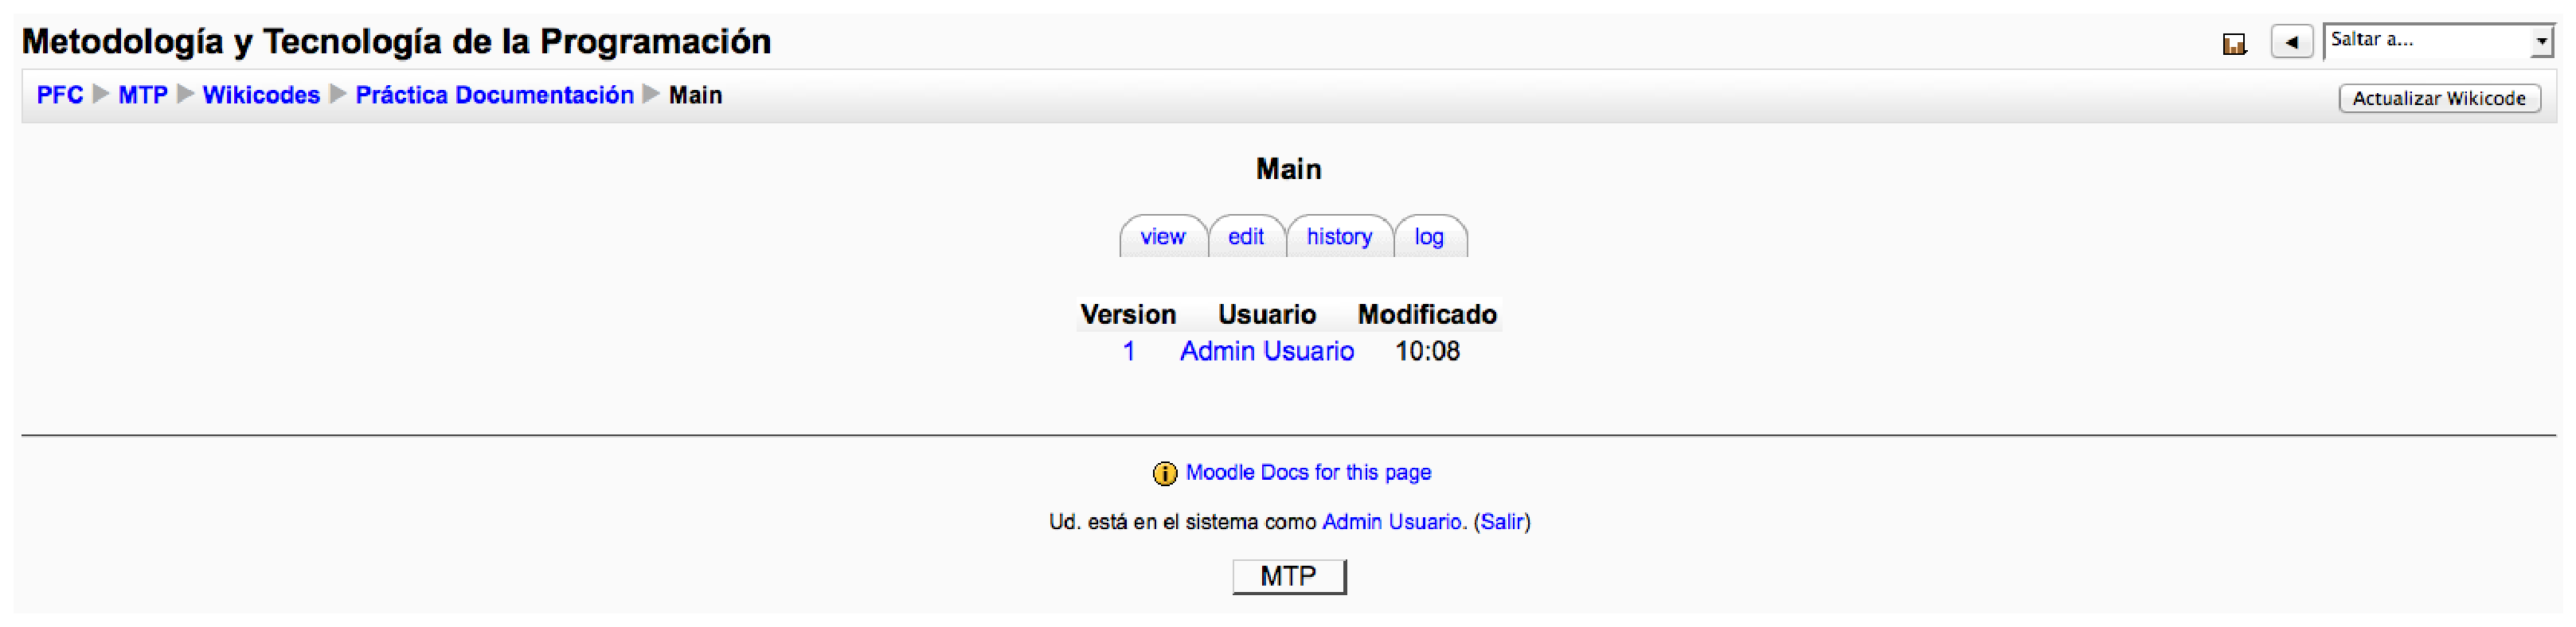
\includegraphics[width=\textwidth]{./img/c4history1.eps}
	\caption{Pantalla histórico Wikicode.}
	\end{center}
\end{figure}

Una vez pulsemos encima de una de estas versiones que se nos ofrece, podremos visualizar el código fuente que había en tal fecha y restaurarlo si así lo vemos oportuno pulsando el enlace a la izquierda de la pantalla. Dicho enlace nos llevará a otro formulario donde se nos pedirá autorización para realizar dicha acción.

\begin{figure}[h]
	\begin{center}
	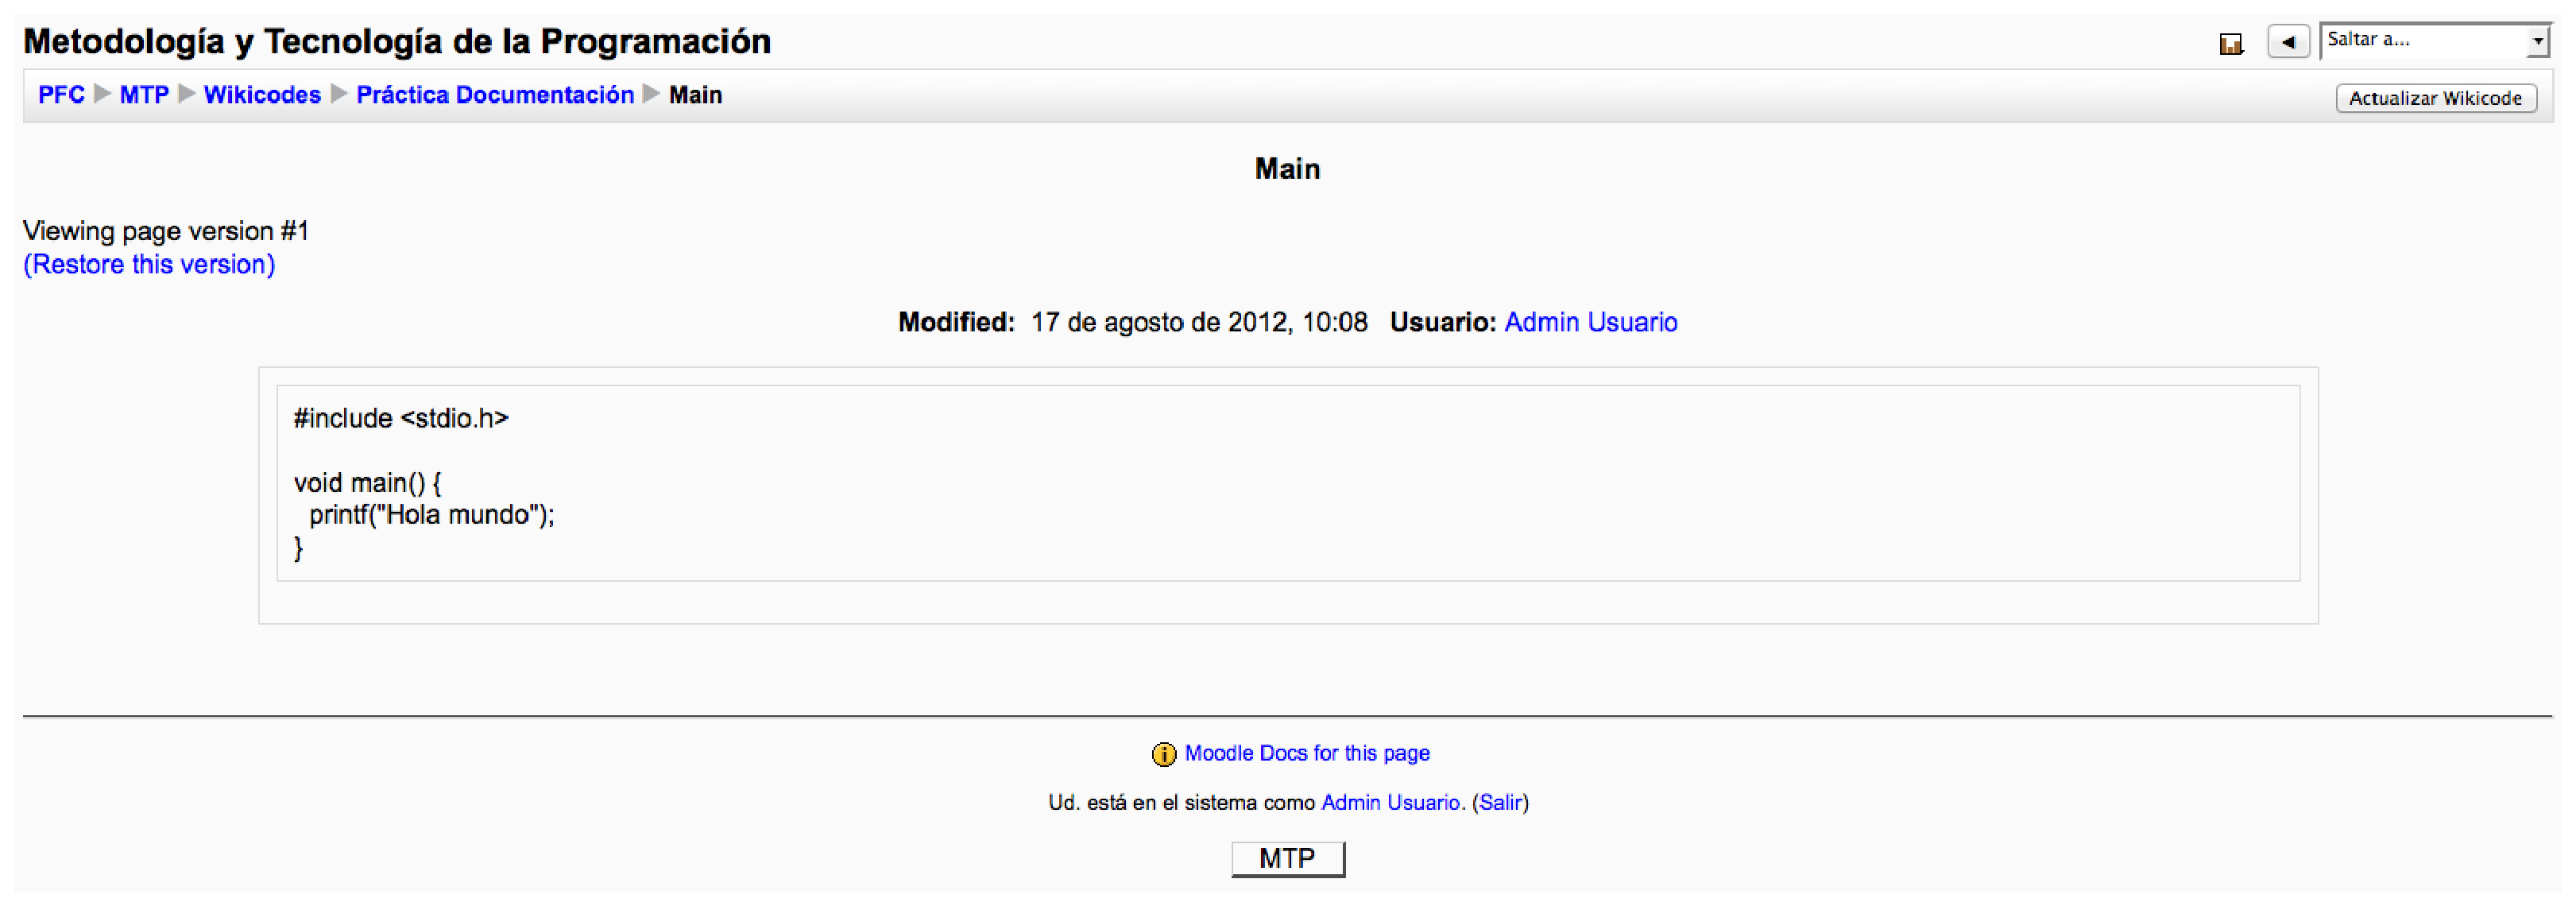
\includegraphics[width=\textwidth]{./img/c4history2.eps}
	\caption{Pantalla restauración histórico Wikicode.}
	\end{center}
\end{figure}

Una de las mayores novedades que presenta el módulo para la versión 2 de Moodle es la inclusión de una potente herramienta que nos permite comparar dos códigos, señalando en el propio interfaz las diferencias entre ambos. El diseño de dicha herramienta se puede ver en la siguiente figura, y para llamarlo habrá que seleccionar dos versiones en la Figura 4.12 y pulsar el botón denominado``Comparar''.

\begin{figure}[h]
	\begin{center}
	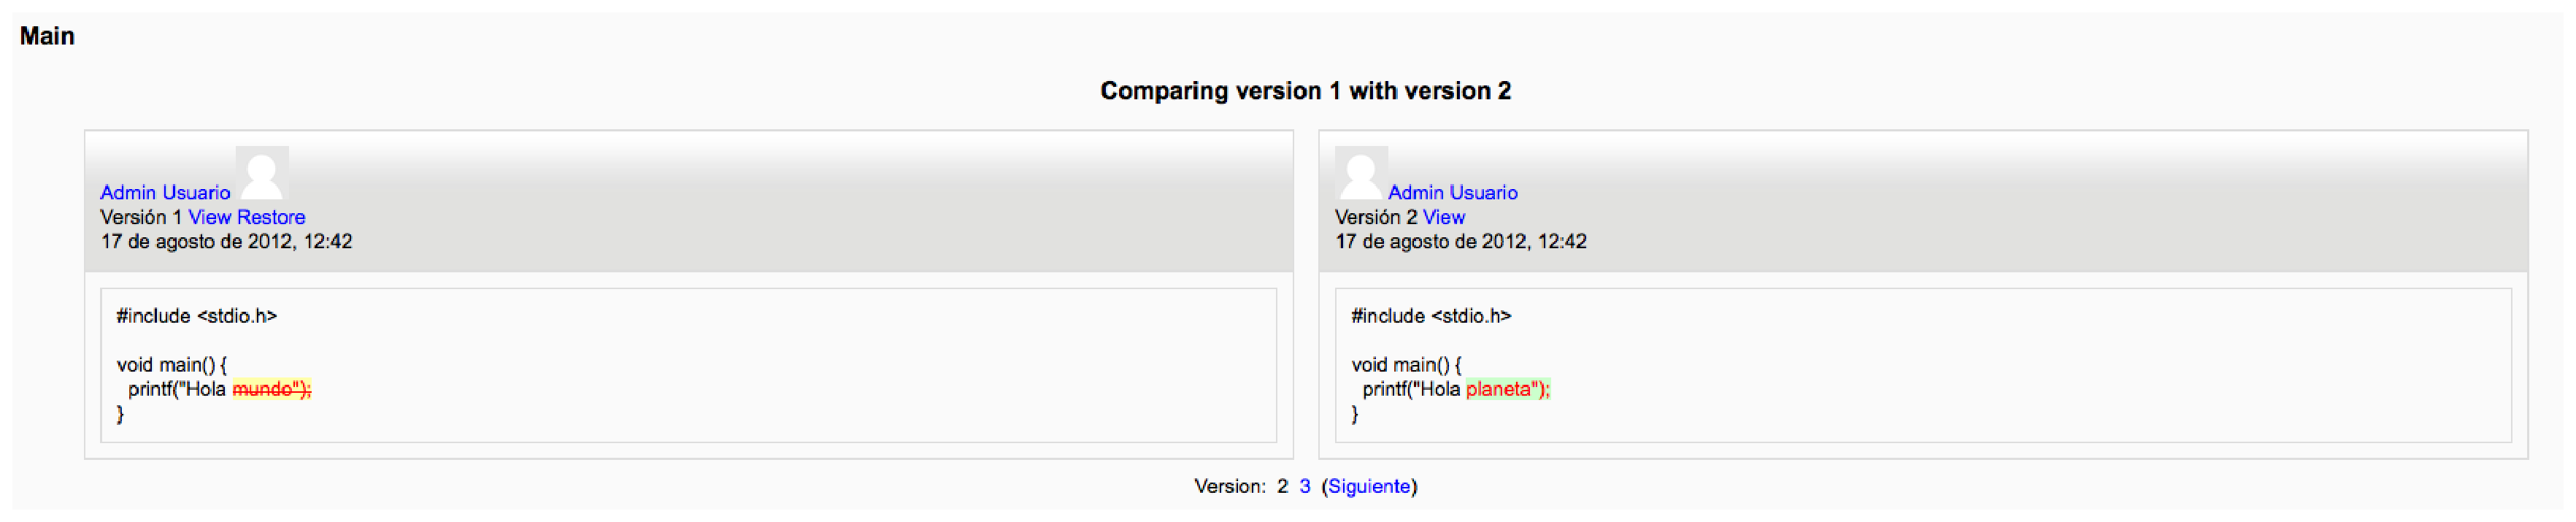
\includegraphics[width=\textwidth]{./img/c4diff.eps}
	\caption{Pantalla comparación histórico Wikicode.}
	\end{center}
\end{figure}

\subsubsection{Pantalla estadísticas}

Este formulario, el último a diseñar, es el que se encargará de traernos la información estadística almacenada en base de datos con respecto al código fuente. Se accede a él pulsando el botón log del menú superior, y una vez dentro de él nos encontraremos una serie de etiquetas con un campo de texto informándonos de su resultado.

Como novedad, a partir de la versión 2 de Moodle se añaden unos botones de ayuda para explicar el significado de cada estadística. El diseño de dicho formulario se puede contemplar en la siguiente figura:

\begin{figure}[h]
	\begin{center}
	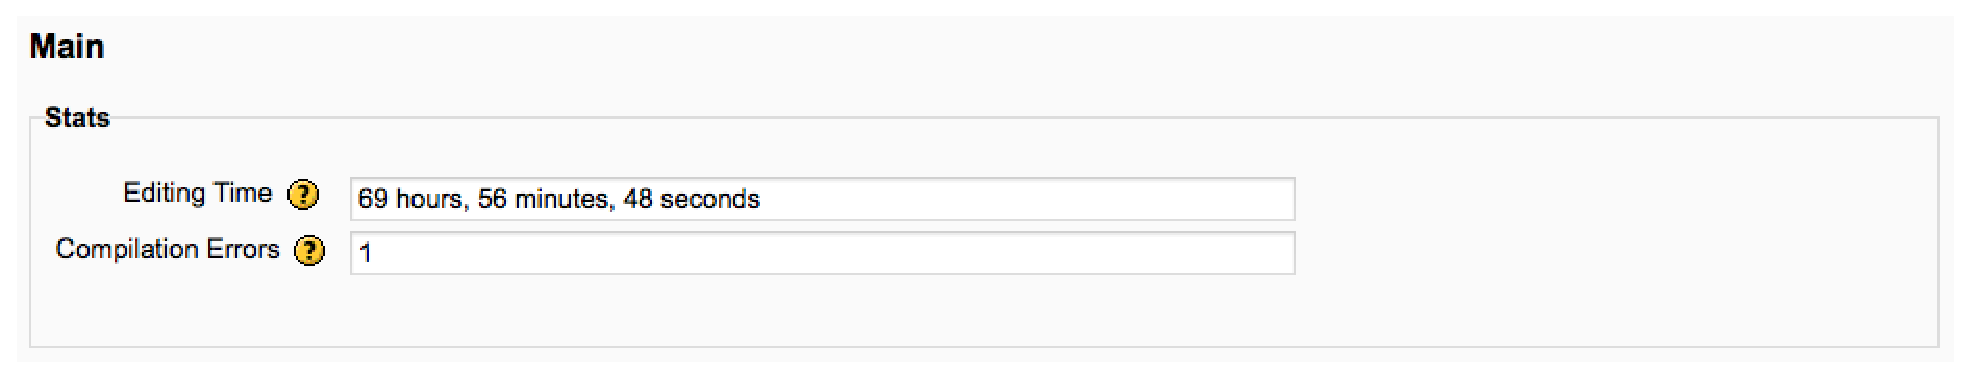
\includegraphics[width=\textwidth]{./img/c4log.eps}
	\caption{Pantalla estadística Wikicode.}
	\end{center}
\end{figure}

\section{Especificación procedimental}

Llegados a este punto, trataremos de modelar el módulo viendo sus aspectos dinámicos desde un alto nivel de abstracción, es decir, nos centraremos en las actividades de negocio más importantes en el dominio del problema. Para ello no pretendemos describir en detalle los procedimientos u operaciones que tienen lugar entre dichos objetos ni los atributos que se intercambian entre sí sino simplemente mostrar las actividades que tienen lugar entre ellos. Para ello, en los siguientes apartados comentaremos los diferentes diagramas de actividades asociados a cada una de los bloques explicados anteriormente.

\subsection{Diagrama de actividades para el sistema Wikicode-Mod}

\subsubsection{Actividad: Crear, configurar y parametrizar la Wikicode}

Una de las principales actividades que debe realizar el \emph{sistema Wikicode-Mod} es la creación de la actividad dentro de Moodle, así como configurarse correctamente para poder usarse en un futuro.

En la siguiente figura se muestra el diagrama de actividades asociado:

\begin{figure}[h]
	\centering
	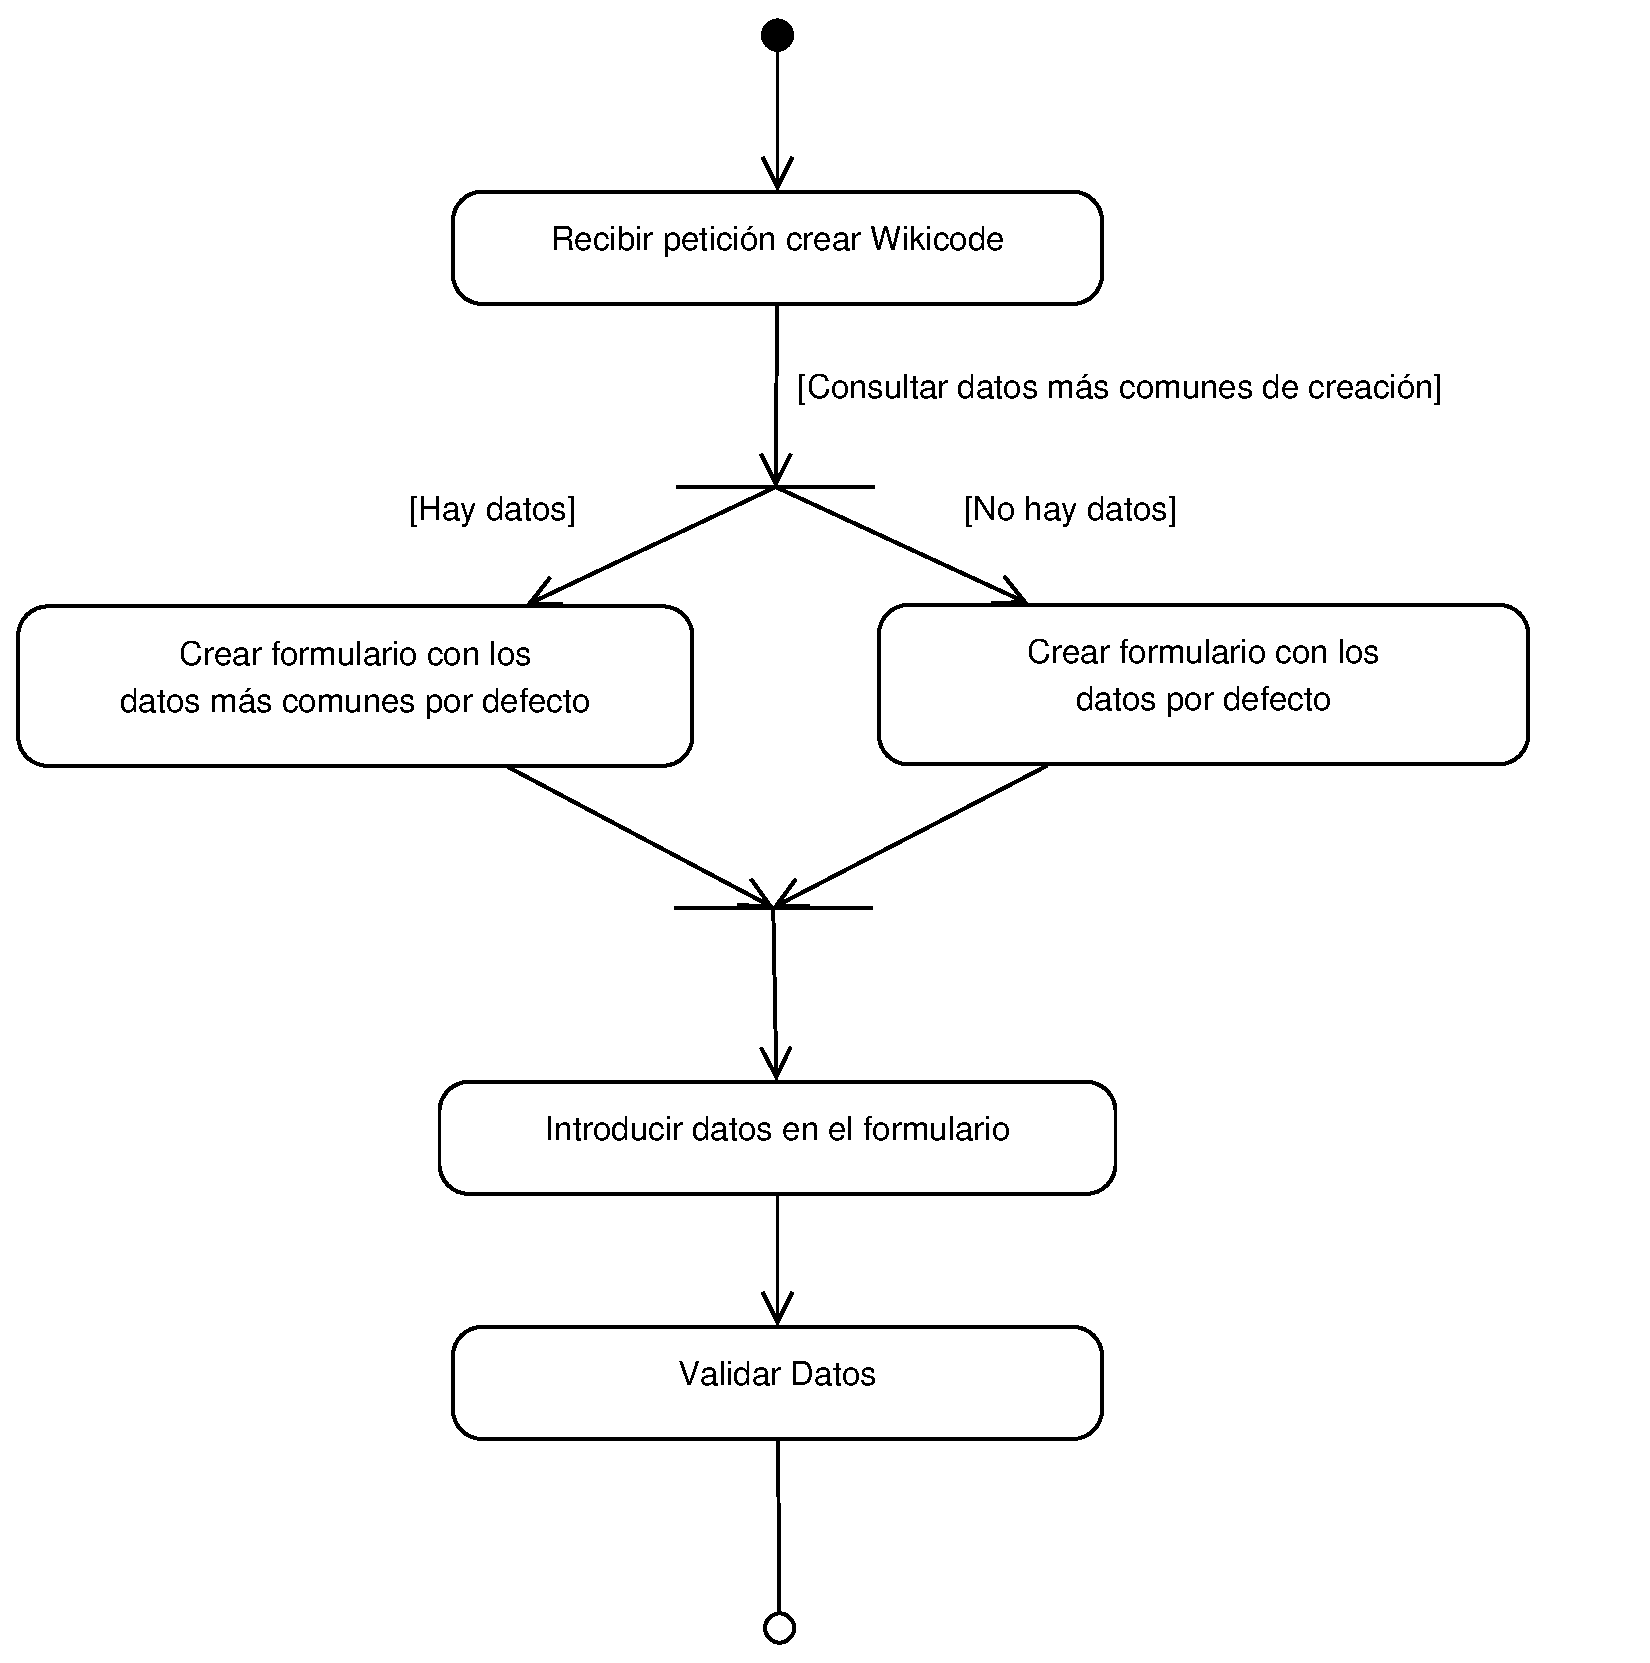
\includegraphics[width=0.7\textwidth]{./img/DiagramaA1.eps}
	\caption{Actividad crear, configurar y parametrizar la Wikicode}
\end{figure}

\newpage
\subsubsection{Actividad: Visualizar código fuente}

Es otra de las actividades que realiza el \emph{sistema Wikicode-Mod}. Se trata de una actividad muy simple en la que se muestra el código fuente de la Wikicode.

El diagrama de actividad es:

\begin{figure}[h]
	\centering
	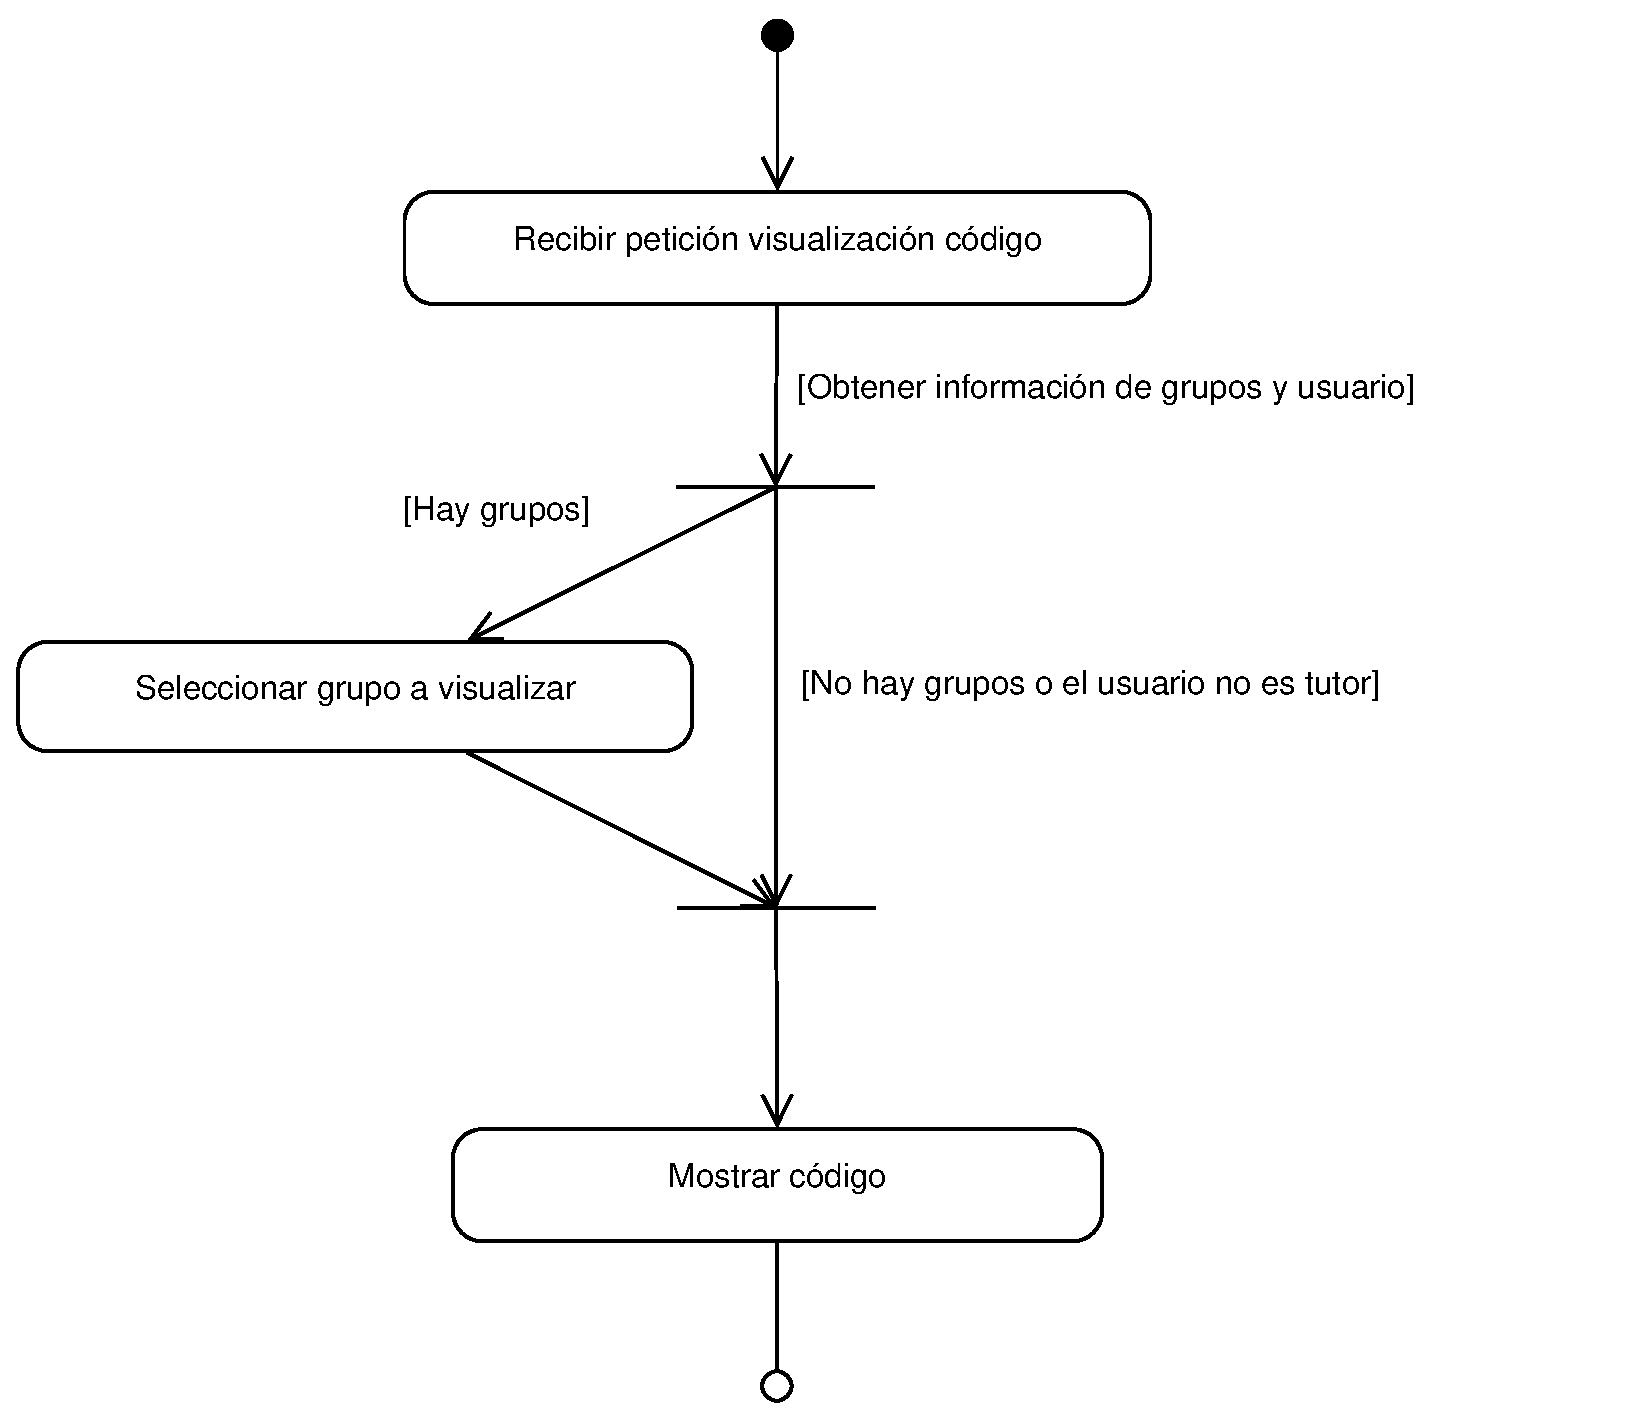
\includegraphics[width=0.7\textwidth]{./img/DiagramaA2.eps}
	\caption{Actividad visualizar código fuente}
\end{figure}

\subsubsection{Actividad: Editar código fuente}

La actividad que nos concierne en este subapartado se trata de la principal labor del \emph{sistema Wikicode-Mod}. Se trata de toda la actividad relacionada con la edición del código fuente, y cómo se almacena en base de datos de manera abstracta al usuario. Las teclas claves están definidas en la especificación de requisitos y la actividad de sincronización se explicará posteriormente.

\newpage

El diagrama de actividad es:

\begin{figure}[h]
	\centering
	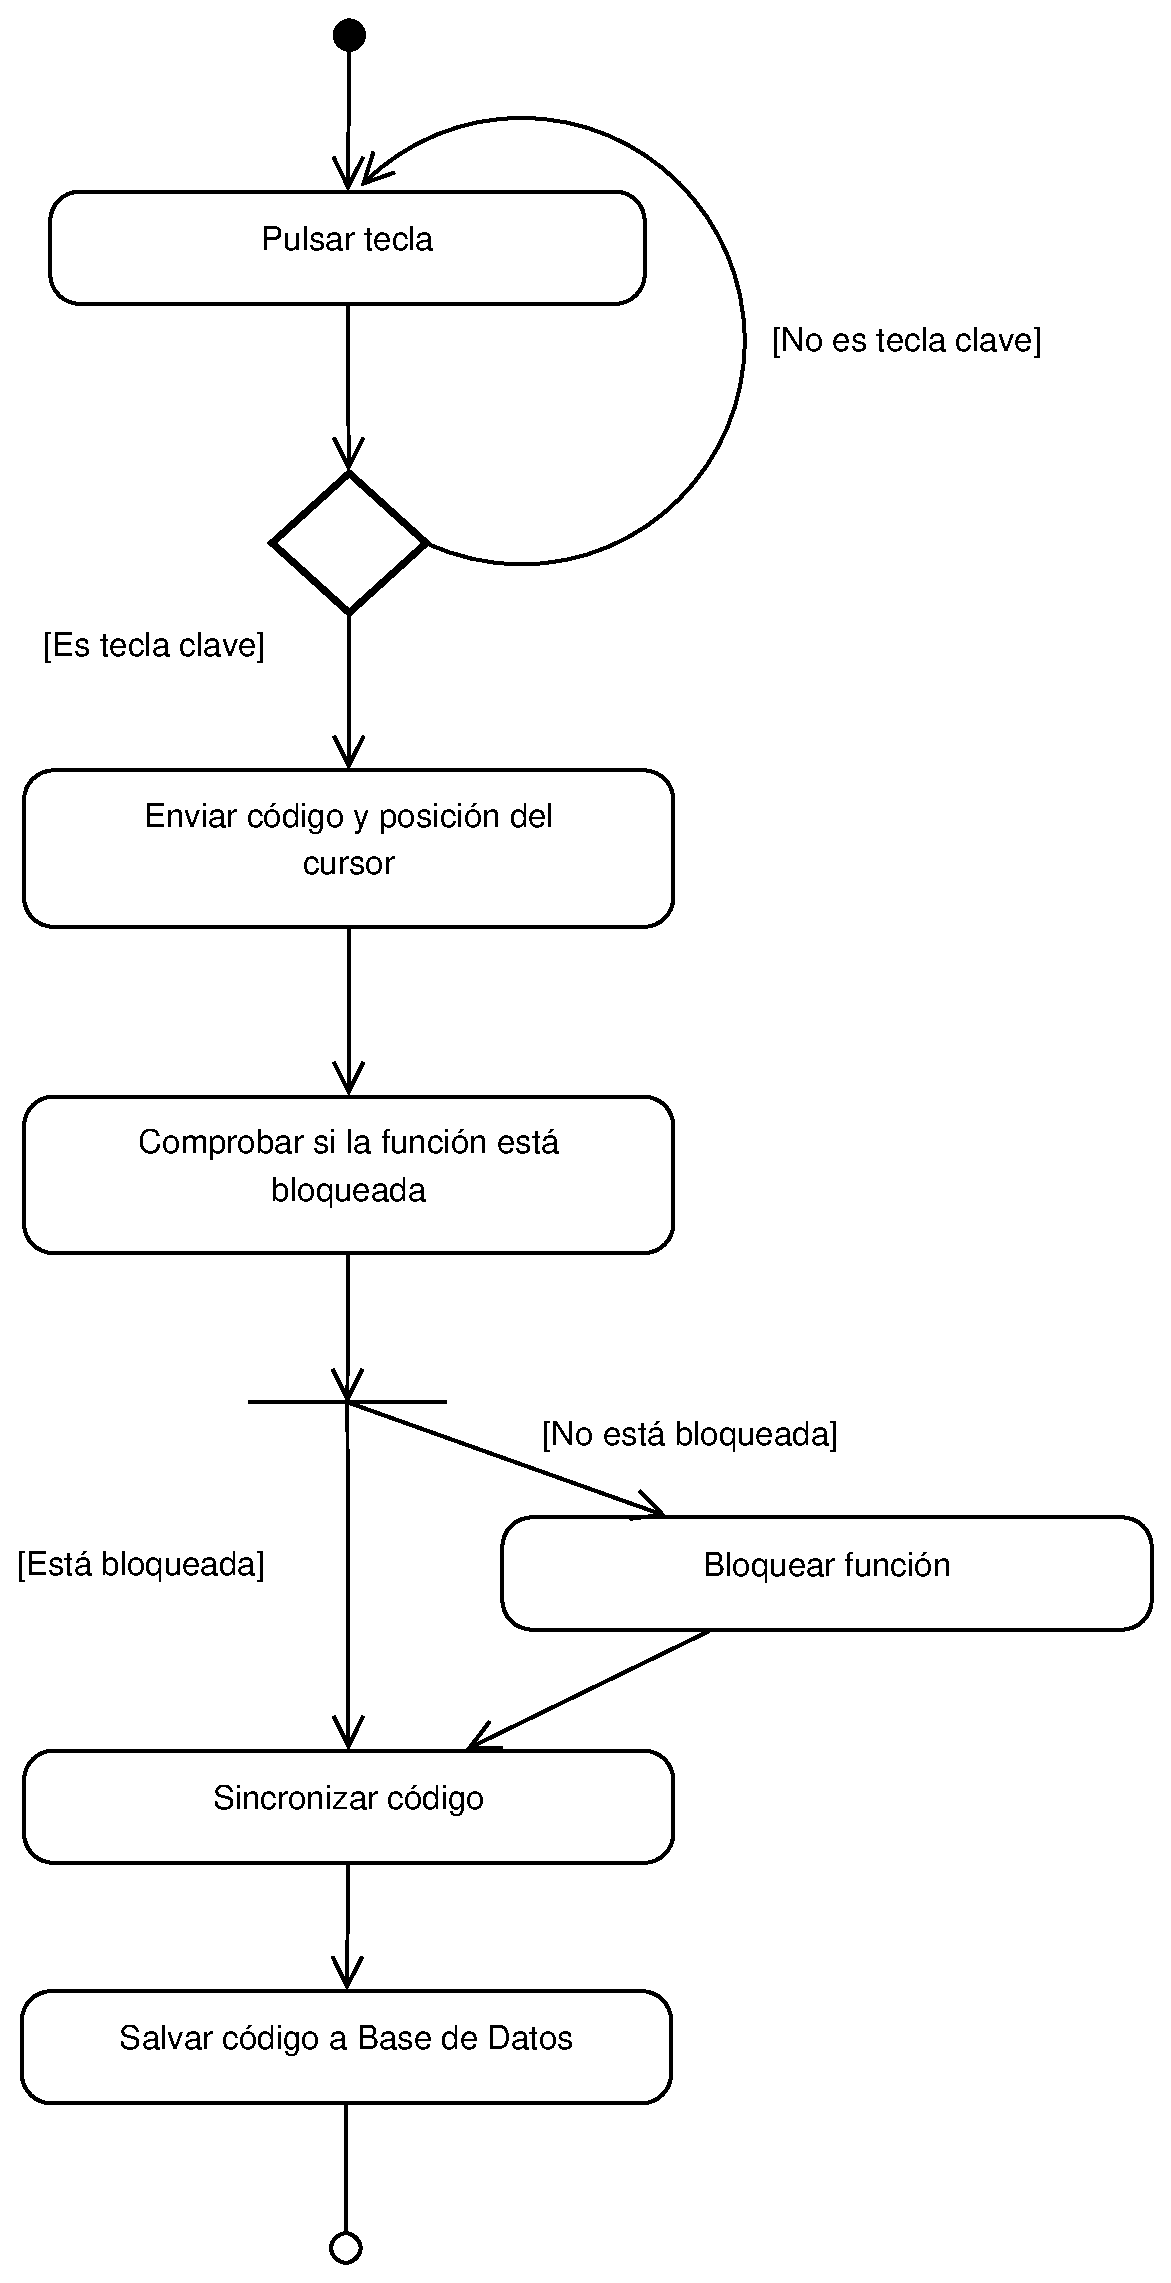
\includegraphics[width=0.54\textwidth]{./img/DiagramaA3.eps}
	\caption{Actividad editar código fuente}
\end{figure}

\newpage

\subsubsection{Actividad: Chat}

El chat es la siguiente actividad que vamos a describir, y es el módulo que utiliza el \emph{sistema Wikicode-Mod} para comunicar a los usuarios entre sí mientras están modificando un código fuente. Es una actividad secuencial en la que únicamente hay que escribir y leer un fichero en un intervalo de tiempo.

En la siguiente figura podemos comprobar el diagrama de actividades asociado al envío de mensajes:

\begin{figure}[h]
	\centering
	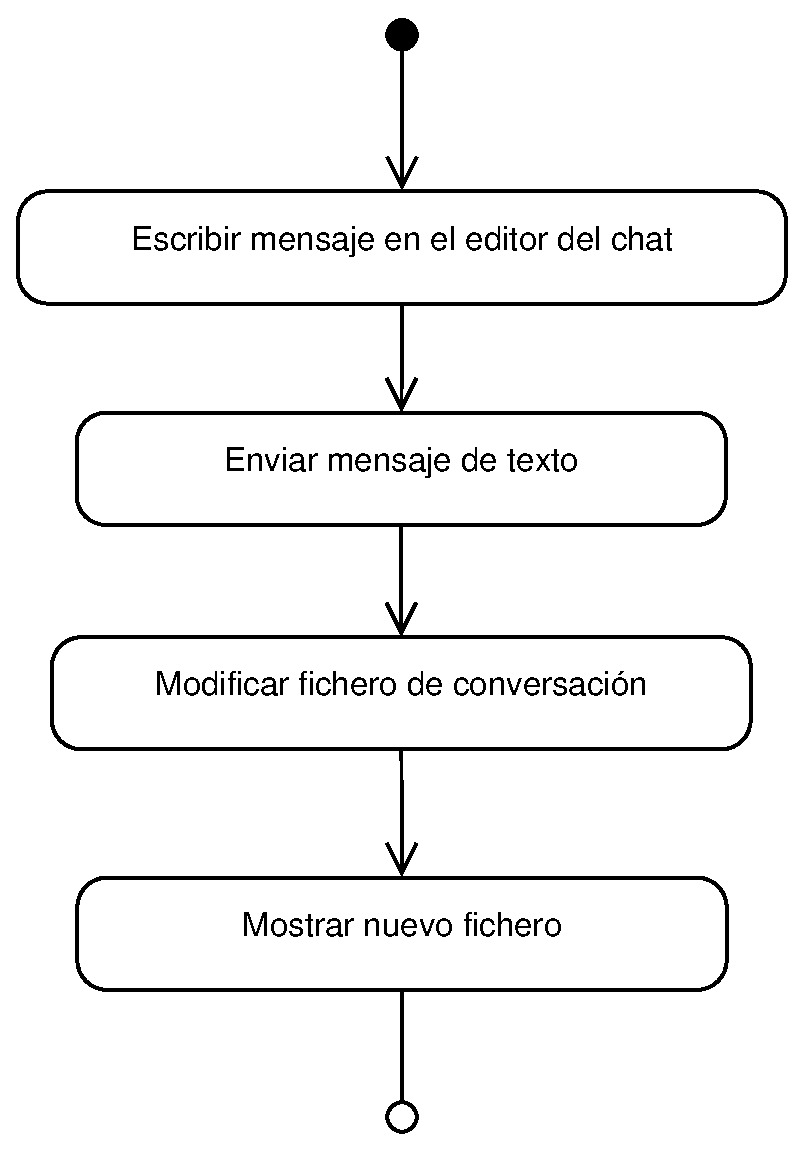
\includegraphics[width=0.4\textwidth]{./img/DiagramaA4.eps}
	\caption{Actividad chat}
\end{figure}

\newpage

\subsubsection{Actividad: Compilar código fuente}

La compilación es el proceso en el que un programa informático, conocido como compilador, traduce un programa escrito en un lenguaje de programación a otro que habitualmente suele ser el lenguaje máquina. En esta actividad el \emph{sistema Wikicode-Mod} tomará el código escrito en el editor y se lo pasará al compilador. Posteriormente podremos comprobar la respuesta de este.

El diagrama de actividad es el siguiente:

\begin{figure}[h]
	\centering
	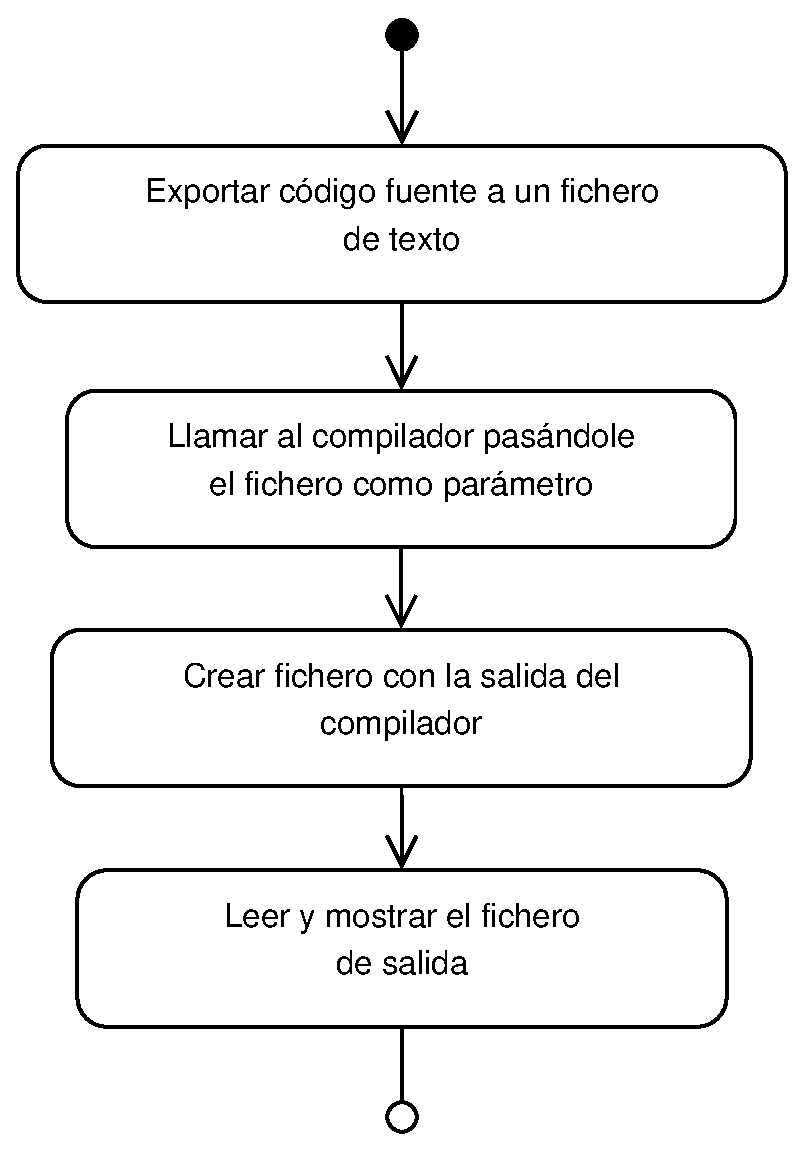
\includegraphics[width=0.4\textwidth]{./img/DiagramaA5.eps}
	\caption{Actividad compilar código fuente}
\end{figure}

\newpage
\subsubsection{Actividad: Visualizar histórico}

Es otra actividad que nos proporciona el \emph{sistema Wikicode-Mod}, en la cual podemos ir viendo toda la historia de un código fuente. Esto nos servirá para, en caso de que hayamos cometido un error, poder hacer un rollback a una versión antigua almacenada. En el histórico no se eliminará ninguna entrada, sino que la que hayamos seleccionado en caso de restauración se creará como una nueva versión. Es decir, sería similar a si hubiéramos copiado todo ese antiguo código y hubiéramos salvado.

Una vez restaurado, volveremos al editor y se podrá volver a editar.

El diagrama de actividad que nos proporciona esta actividad se muestra en la siguiente figura:

\begin{figure}[h]
	\centering
	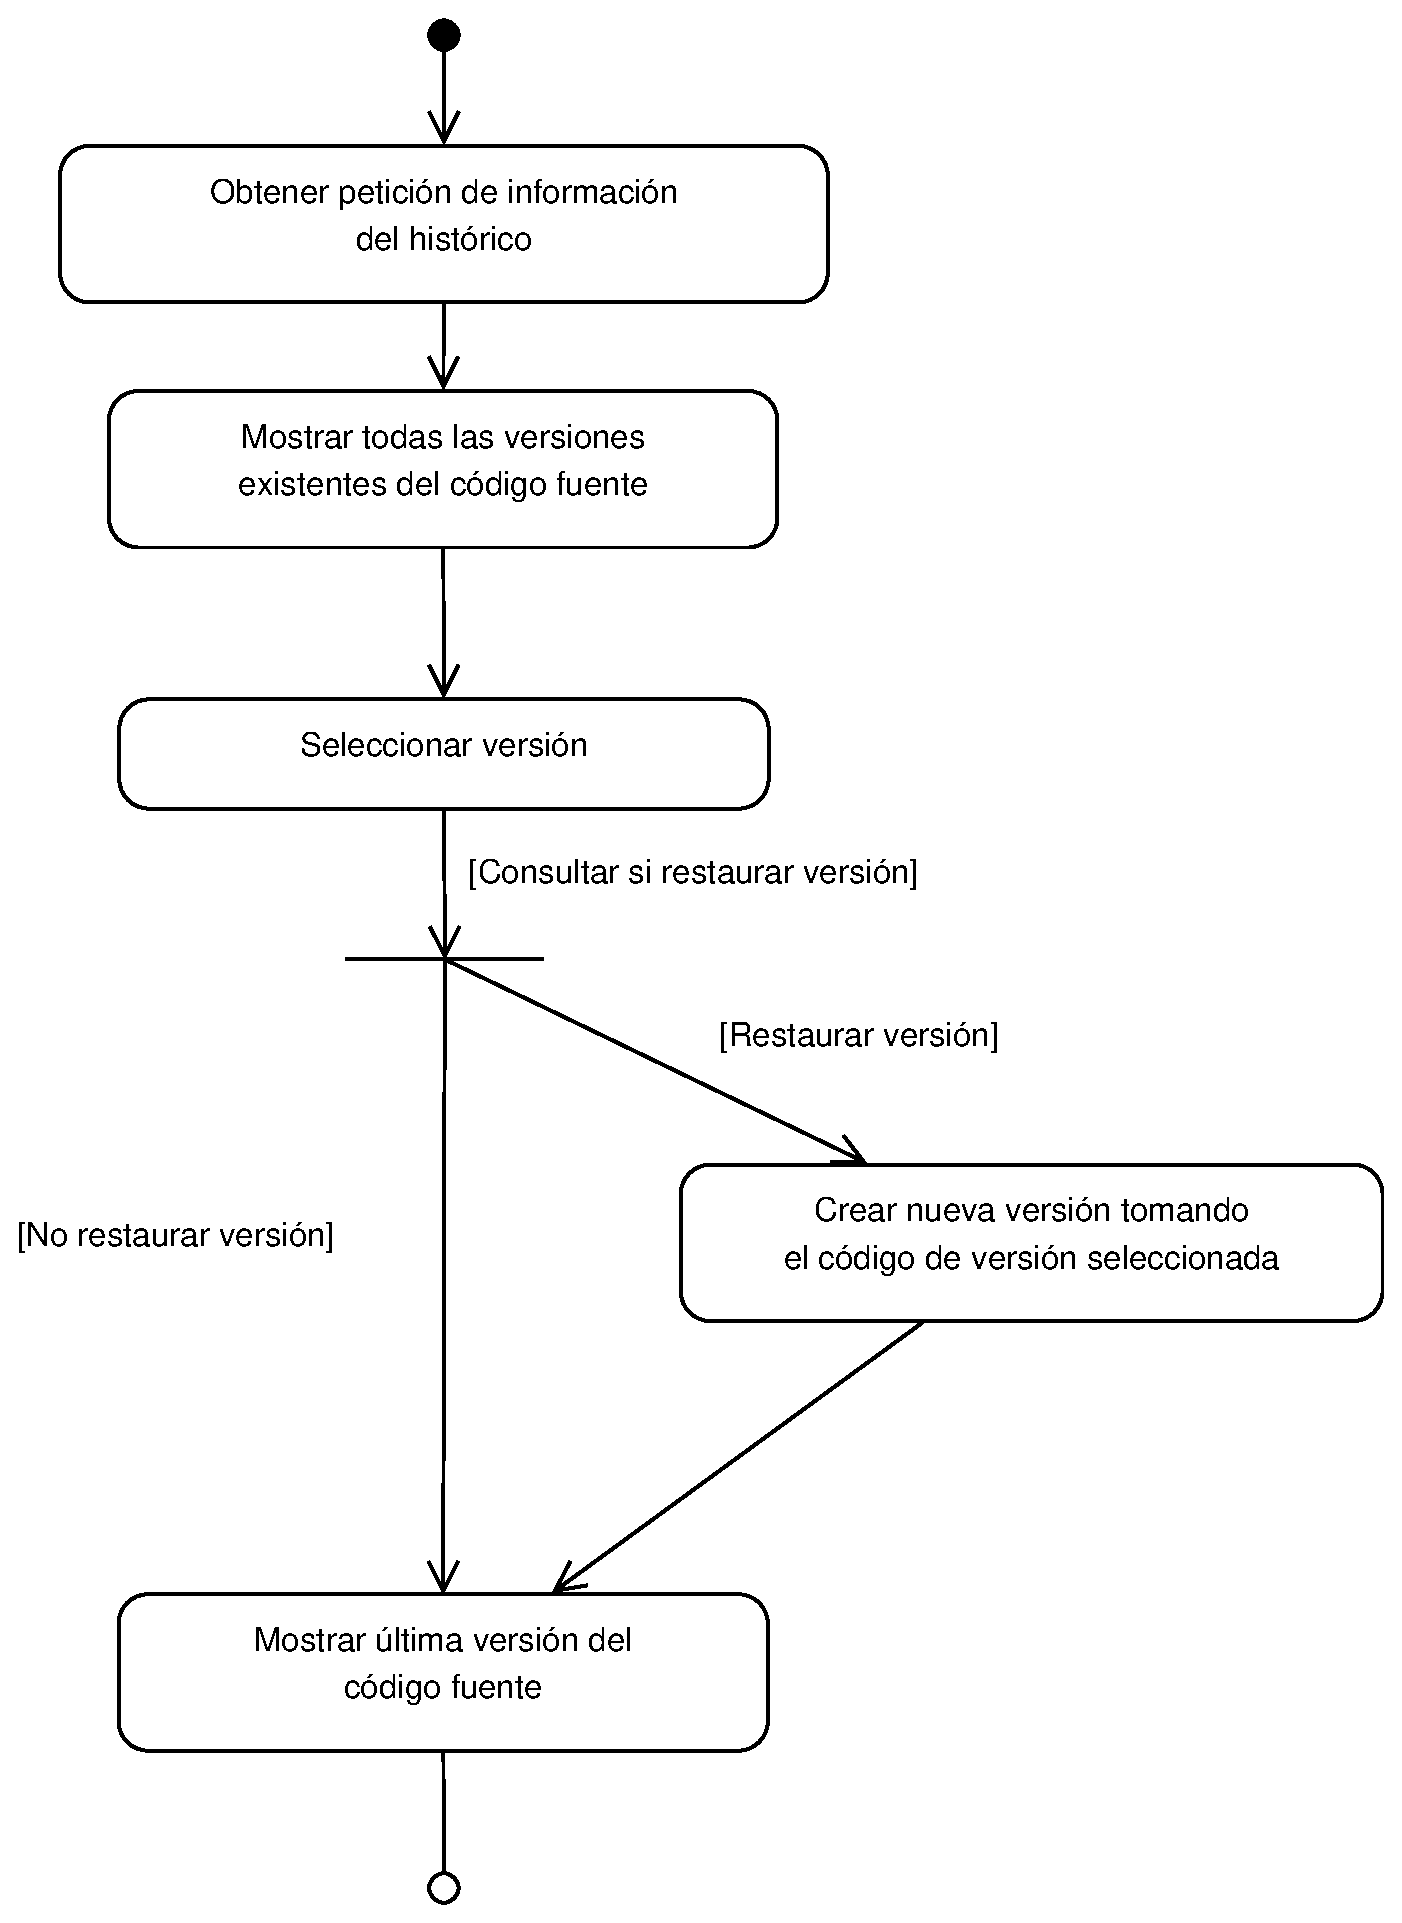
\includegraphics[width=0.6\textwidth]{./img/DiagramaA8.eps}
	\caption{Actividad visualizar histórico}
\end{figure}

\newpage
\subsubsection{Actividad: Visualizar estadísticas}

Es otra actividad del \emph{sistema Wikicode-Mod} puede ser una de las más utilizadas por los tutores para poder valorar la realización de prácticas de programación. En ella se puede consultar todo lo referente en torno a la programación de una actividad \emph{Wikicode} y se puede ampliar en un futuro con tantas estadísticas como se desee sin necesidad de variar el diagrama de actividad.

El diagrama de actividad se muestra en la siguiente figura:

\begin{figure}[h]
	\centering
	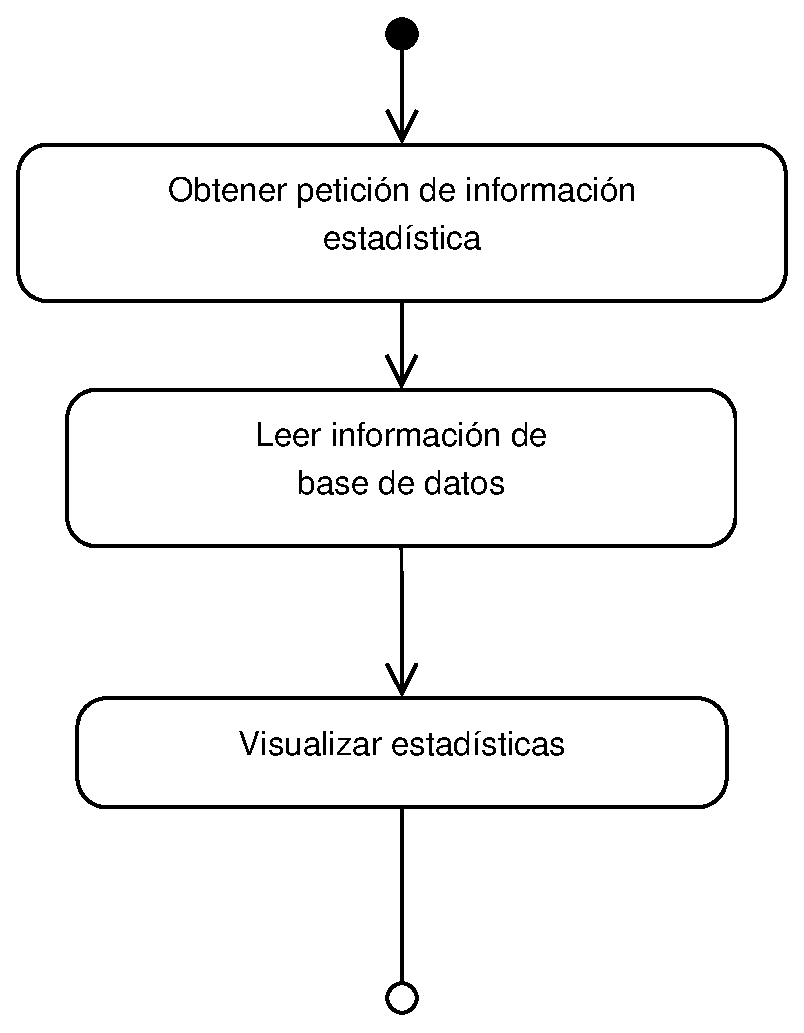
\includegraphics[width=0.5\textwidth]{./img/DiagramaA9.eps}
	\caption{Actividad visualizar estadísticas}
\end{figure}

\newpage
\subsection{Diagrama de actividades para el sistema Wikicode-Synchronizer}
\subsubsection{Actividad: Sincronizar código}

La sincronización de código es el procedimiento en el que se toma las variaciones del código fuente de un usuario y se pone en consonancia con el resto de usuarios. Del mismo modo, en ese mismo proceso se conseguirá tomar las variaciones de los otros usuarios para poder mostrárselo al usuario que está modificando su código. Así, se tratará de un proceso para poder ir viendo en tiempo real todas las modificaciones que va habiendo en un código sin necesidad de pisar el trabajo entre sí de los usuarios.

En la siguiente figura podemos comprobar el diagrama de actividades asociado a la sincronización del código fuente de un usuario con los demás:

\begin{figure}[h]
	\centering
	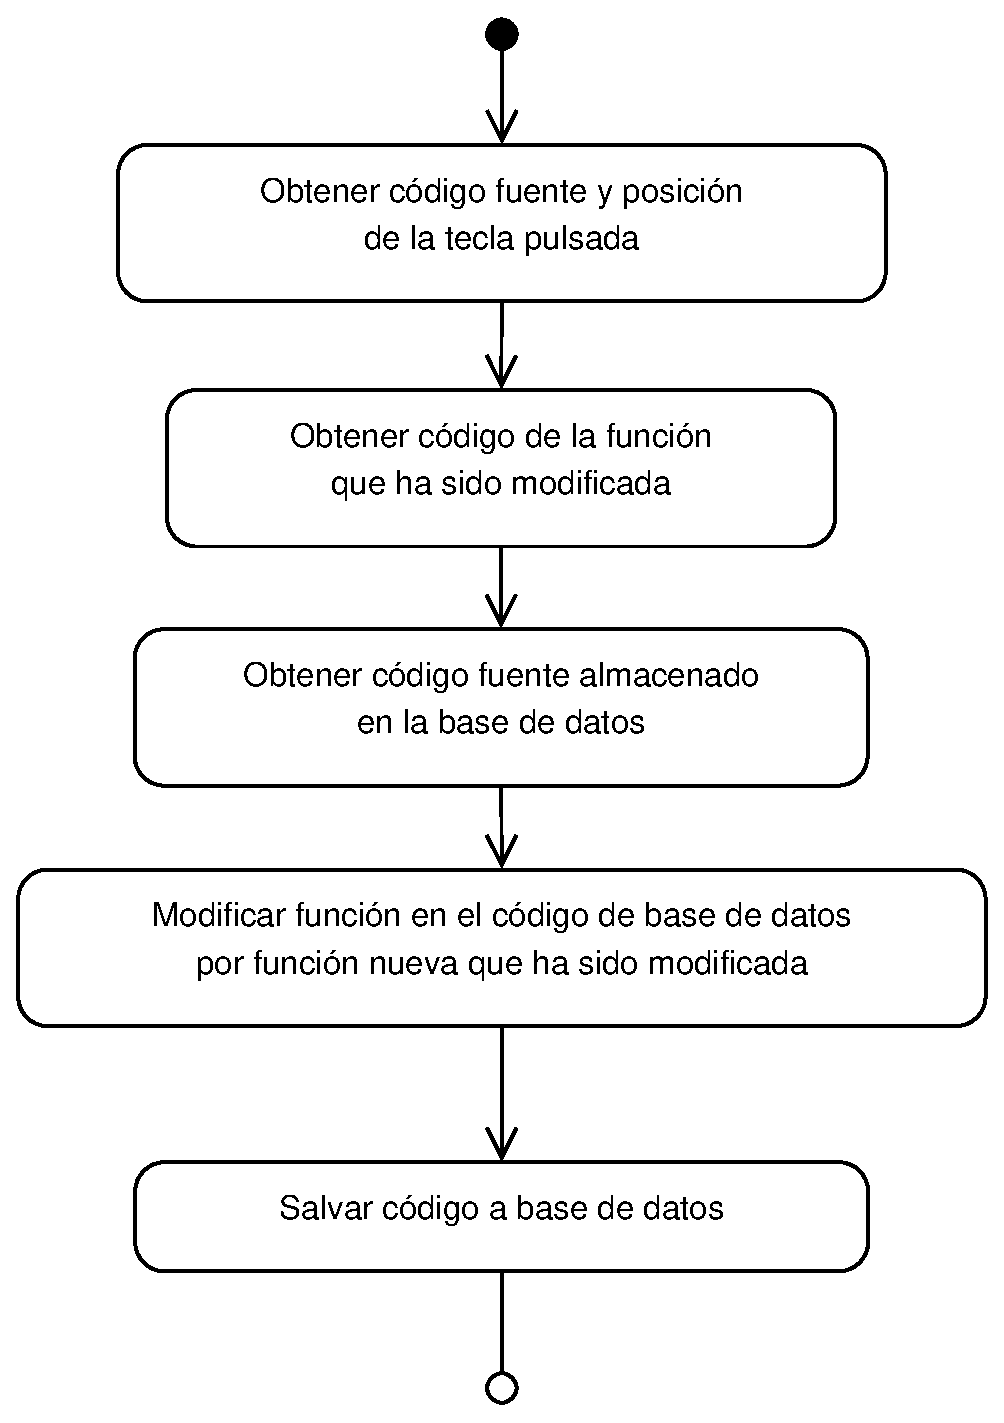
\includegraphics[width=0.5\textwidth]{./img/DiagramaA6.eps}
	\caption{Actividad sincronizar código}
\end{figure}

\newpage
\subsubsection{Actividad: Actualizar estadísticas}

Como se ha mostrado en la Figura 4.22, el usuario tendrá la posibilidad de consultar las estadísticas sobre su página de código. Estas estadísticas no son calculadas a la hora de realizar la consulta, sino que se van almacenando y actualizando en base de datos conforme se van produciendo, de este modo la carga de la operación de consulta es mucho menor y las operaciones únicamente son necesarias de realizar una vez. 

En el siguiente diagrama se muestra como se van calculando dichas estadísticas y almacenando en base de datos:

\begin{figure}[h]
	\centering
	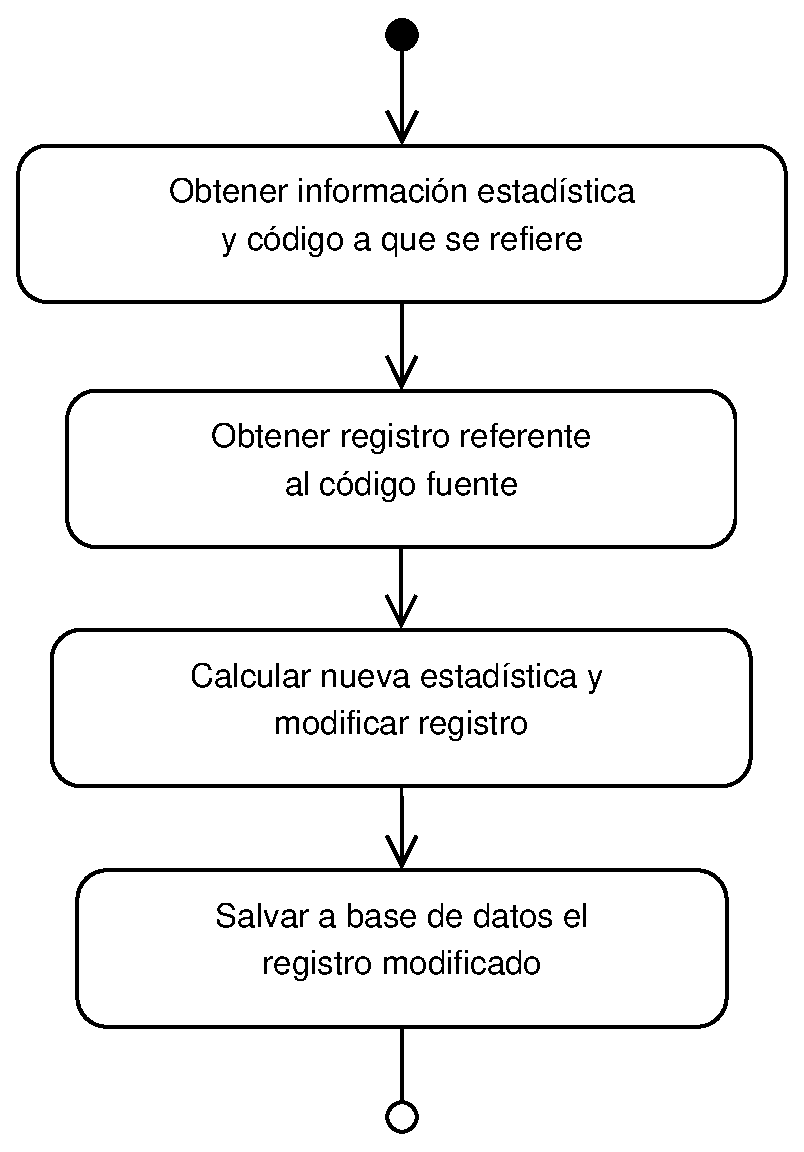
\includegraphics[width=0.4\textwidth]{./img/DiagramaA7.eps}
	\caption{Actividad actualizar estadísticas}
\end{figure}

\newpage

\section{Modelo de paquetes}

Para una mejor compresión de la arquitectura del sistema, los elementos del modelo de objetos se agrupan en paquetes. Un paquete organiza los objetos en grupos de modo que puedan ser manipulados de forma global. Cada paquete agrupa elementos cercanos semánticamente y funcionalmente. La visibilidad de los elementos del paquete va implícita en la propia especificación de cada elemento.

La interfaz del paquete la conforman todos aquellos elementos que son visibles fuera del paquete. Cada paquete posee un nombre único dentro del sistema. Un paquete puede contener subpaquetes cuyo nombre va precedido del nombre del paquete contenedor. Cada objeto pertenece exclusivamente a un único paquete. Un paquete forma un espacio de nombres, lo que significa que la nomenclatura de los elementos del mismo grupo no debe repetirse en el contexto de su paquete contenedor. Un paquete puede importar la interfaz de otro paquete para acceder a sus elementos. Esta importación es un permiso explícito de acceso en un solo sentido.

Un paquete puede ser representado gráficamente como una proyección de su modelo de contenido. Para la representación de cada paquete se hará uso de la notación gráfica de UML 2.0.

Para el caso de este proyecto tenemos una arquitectura cliente-servidor, por tanto se debe hacer una separación clara entre la interfaz de usuario del sistema que reside en el cliente y los datos persistentes del sistema que residen en el servidor.

\subsection{Paquete Cliente de Wikicode}

Este paquete representa el bloque cliente de la arquitectura. El bloque cliente visto desde el punto de vista físico estará formado por al menos un terminal que estará ejecutando la plataforma Moodle remotamente (navegador). Este terminal estará conectado con un servidor que será el módulo de Moodle que aceptará las peticiones del usuario.

\subsection{Paquete Servidor/Cliente Wikicode-Mod de Wikicode}

Esta parte representa al módulo de Moodle que actúa como servidor aceptando las peticiones del usuario y sirviendo de interfaz de entrada para la edición de código. Sin embargo, este servidor también actuará como cliente pues será el que realice las peticiones de sincronización de datos y salvado en base de datos. 

De esta manera, este módulo servidor/cliente deberá hacer lo siguiente:

\begin{itemize}
	\item Aceptar las peticiones del usuario.
	\item Obtener los registros de base de datos conforme a las peticiones de los usuarios.
	\item Hacer de interfaz de entrada a la hora de edición del código fuente.
	\item Enviar la petición de sincronización de código mediante un paquete JSon y el método Get\footnote{\textbf{Get: }Método de petición HTTP el cual pide una representación del recurso especificado.}.
	\item Enviar la petición de escritura en la conversación agrupada como chat mediante el método Post\footnote{\textbf{Post: }Método de petición HTTP el cual somete los datos a que sean procesados para el recurso identificado. Los datos se incluirán en el cuerpo de la petición.}.
	\item Llamar al compilador externo y leer la salida del fichero de intercambio.
\end{itemize}

La finalidad de este bloque es realizar una separación entre la aplicación que maneja la sincronización del código fuente y el sistema de gestión de cursos consiguiendo la independencia de ambos. Esta independencia es fundamental pues permite utilizar la aplicación de sincronización para cualquier otra plataforma que no sea Moodle.

\subsection{Paquete Servidor Wikicode-Synchronizer de Wikicode} 

El tercer bloque consiste en una clase que recoge el código y la posición del carácter modificado y la petición de sincronización o bloqueo. Una vez recogida la información, realiza los algoritmos necesarios para sincronizar el código fuente para que actúe de modo colaborativo. Una vez los datos se han sincronizado se almacenan en base de datos para que el bloque \emph{Wikicode-Mod} pueda tener acceso a ellos siempre que los necesite. También se enviará la información sincronizada como un paquete JSON para que dicho bloque no tenga que acceder de manera secuencial a base de datos.

\newpage
\subsection{Diagrama de paquetes}

El diagrama de paquetes correspondiente es el siguiente:

\begin{figure}[h]
	\centering
	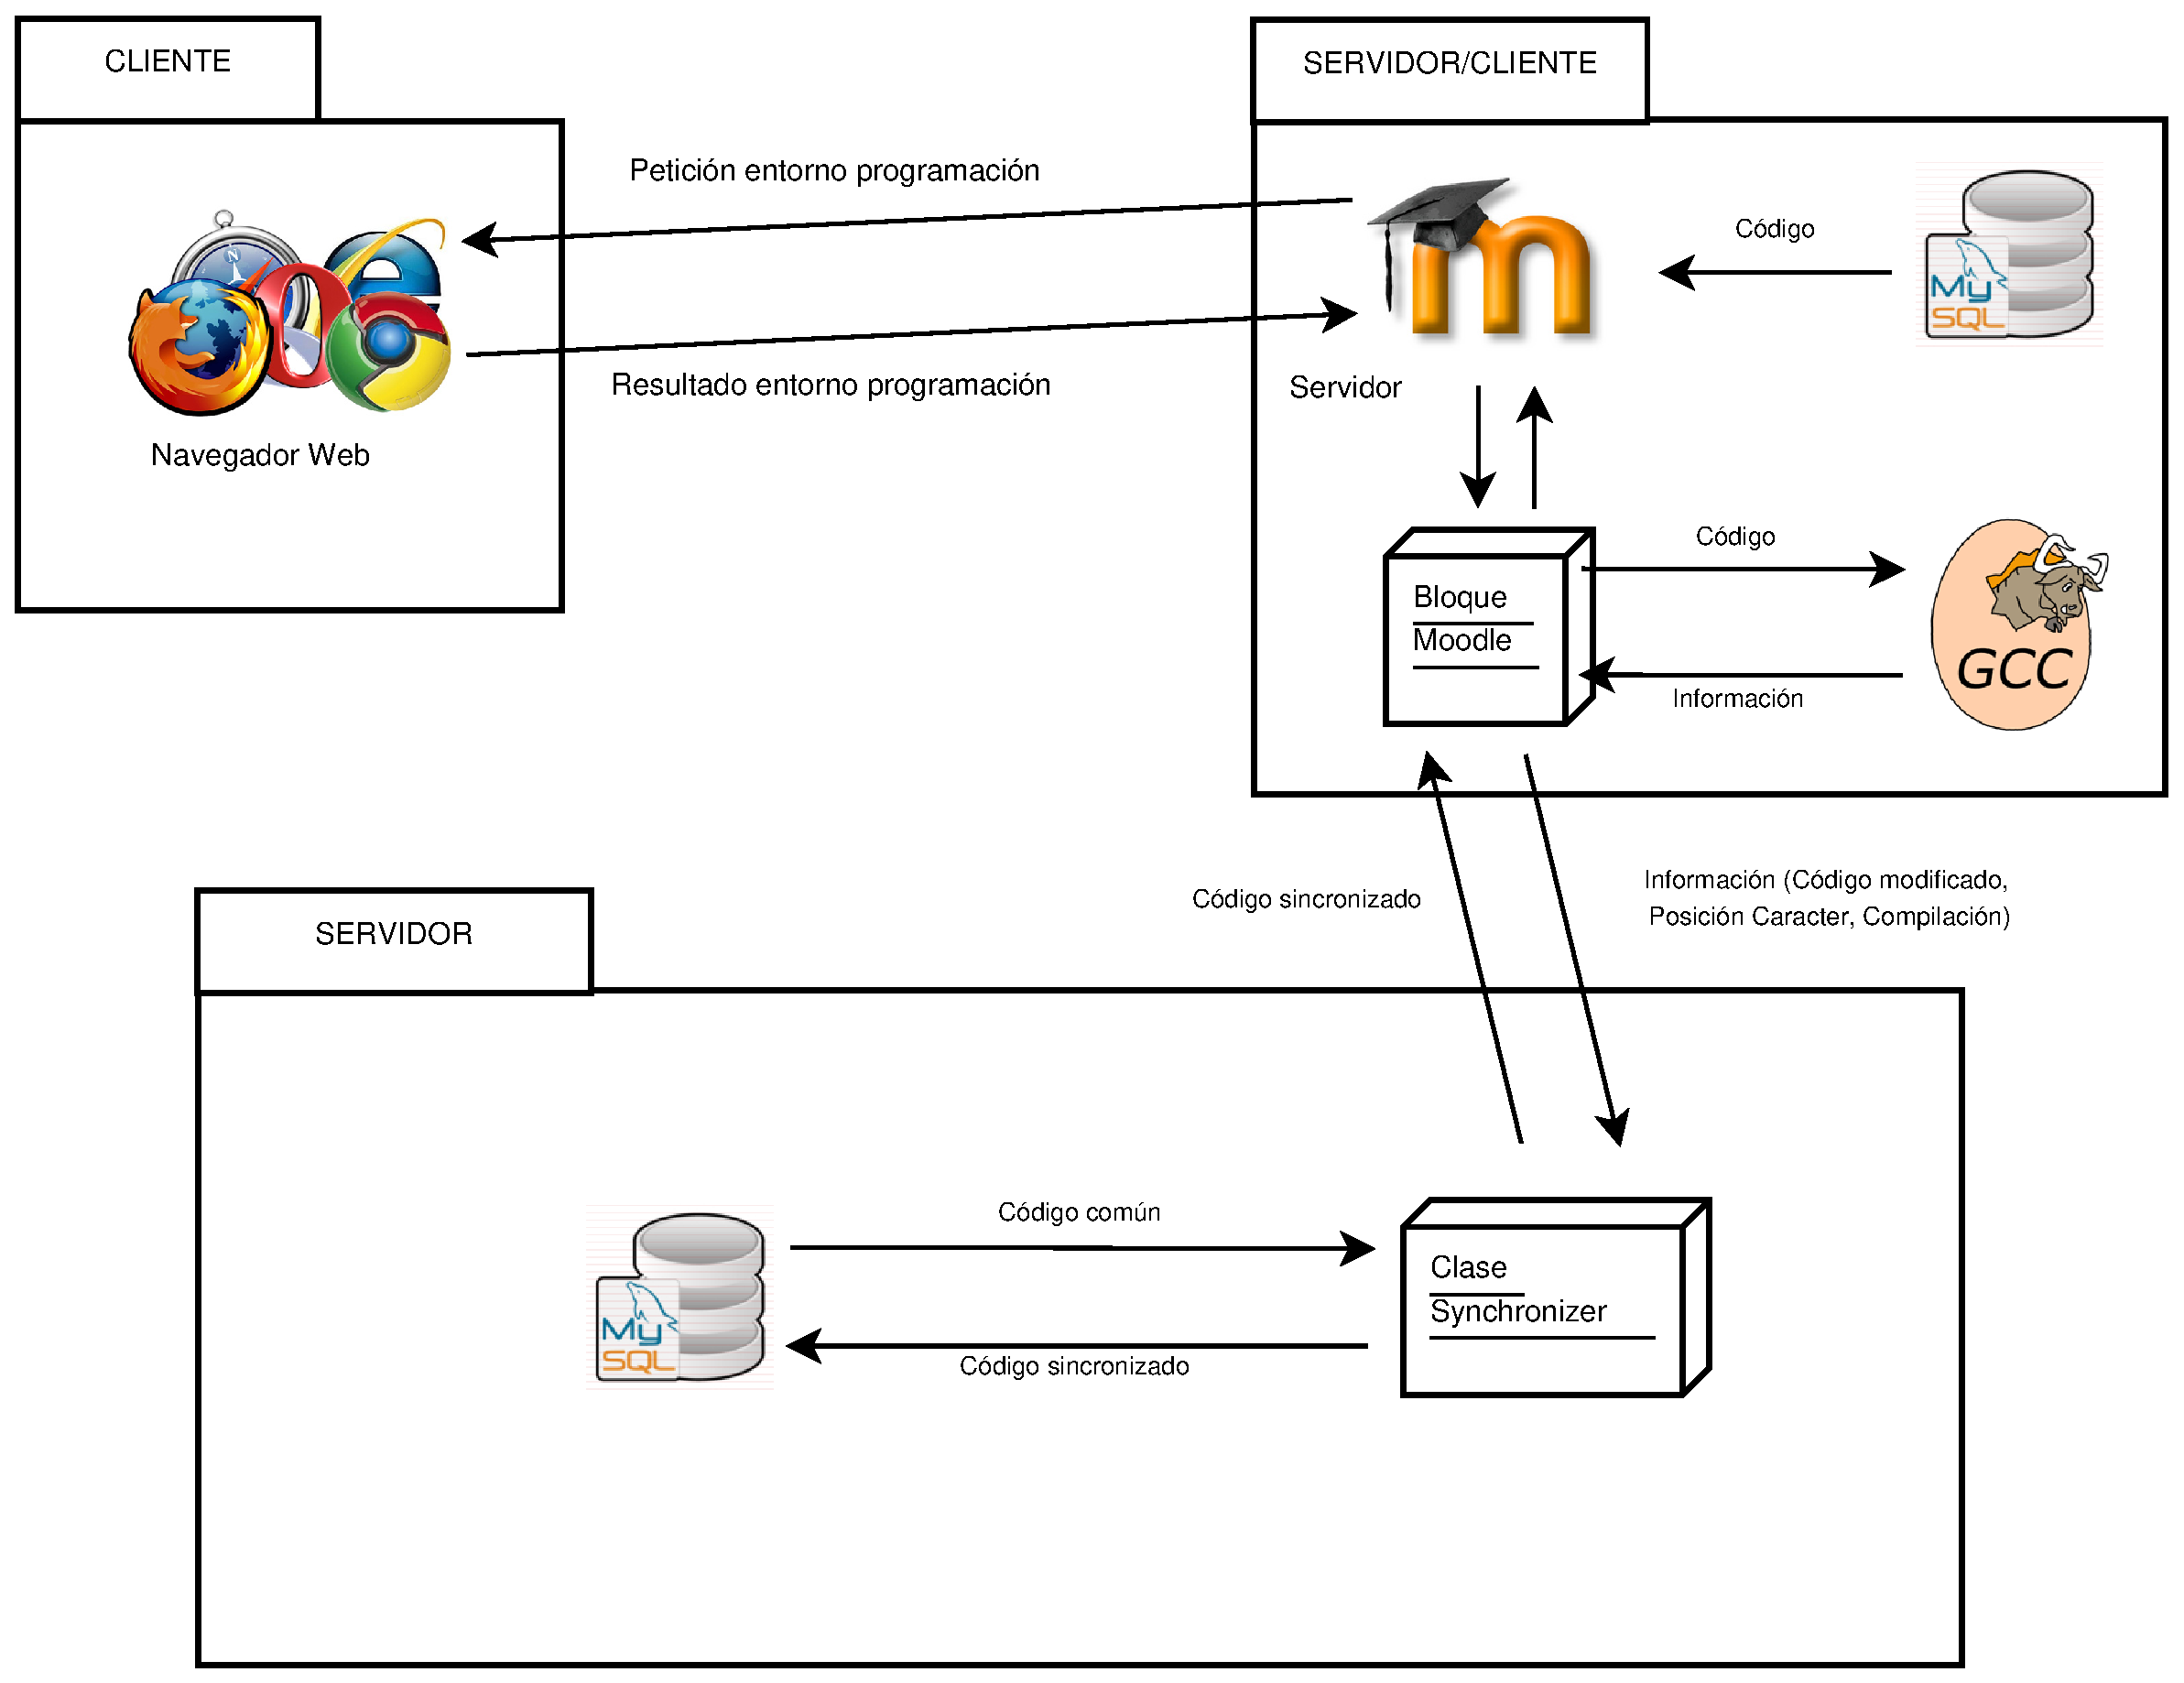
\includegraphics[width=\textwidth]{./img/diagramapaquetes.eps}
	\caption{Diagrama de paquetes}
\end{figure}



















































	%!TEX root=./pfc.tex
\chapter[Implementación del sistema]{\label{}
Implementación del sistema}

La vista de implementación se ocupa de la gestión de la configuración de las partes del sistema (componentes), las cuales pueden ensamblarse de diferentes formas para obtener el sistema ejecutable.

De esta manera, los diagramas de componentes aparecen cuando se modelan los aspectos físicos de los sistemas orientados a objetos. Así, los diagramas de componentes muestran la organización y las dependencias entre un conjunto de componentes y se utilizan para modelar la vista de implementación estática de un sistema.

Por tanto, ahora se va a comentar el diagrama de componentes asociado al sistema para especificar la implementación del sistema.

\begin{figure}[h]
	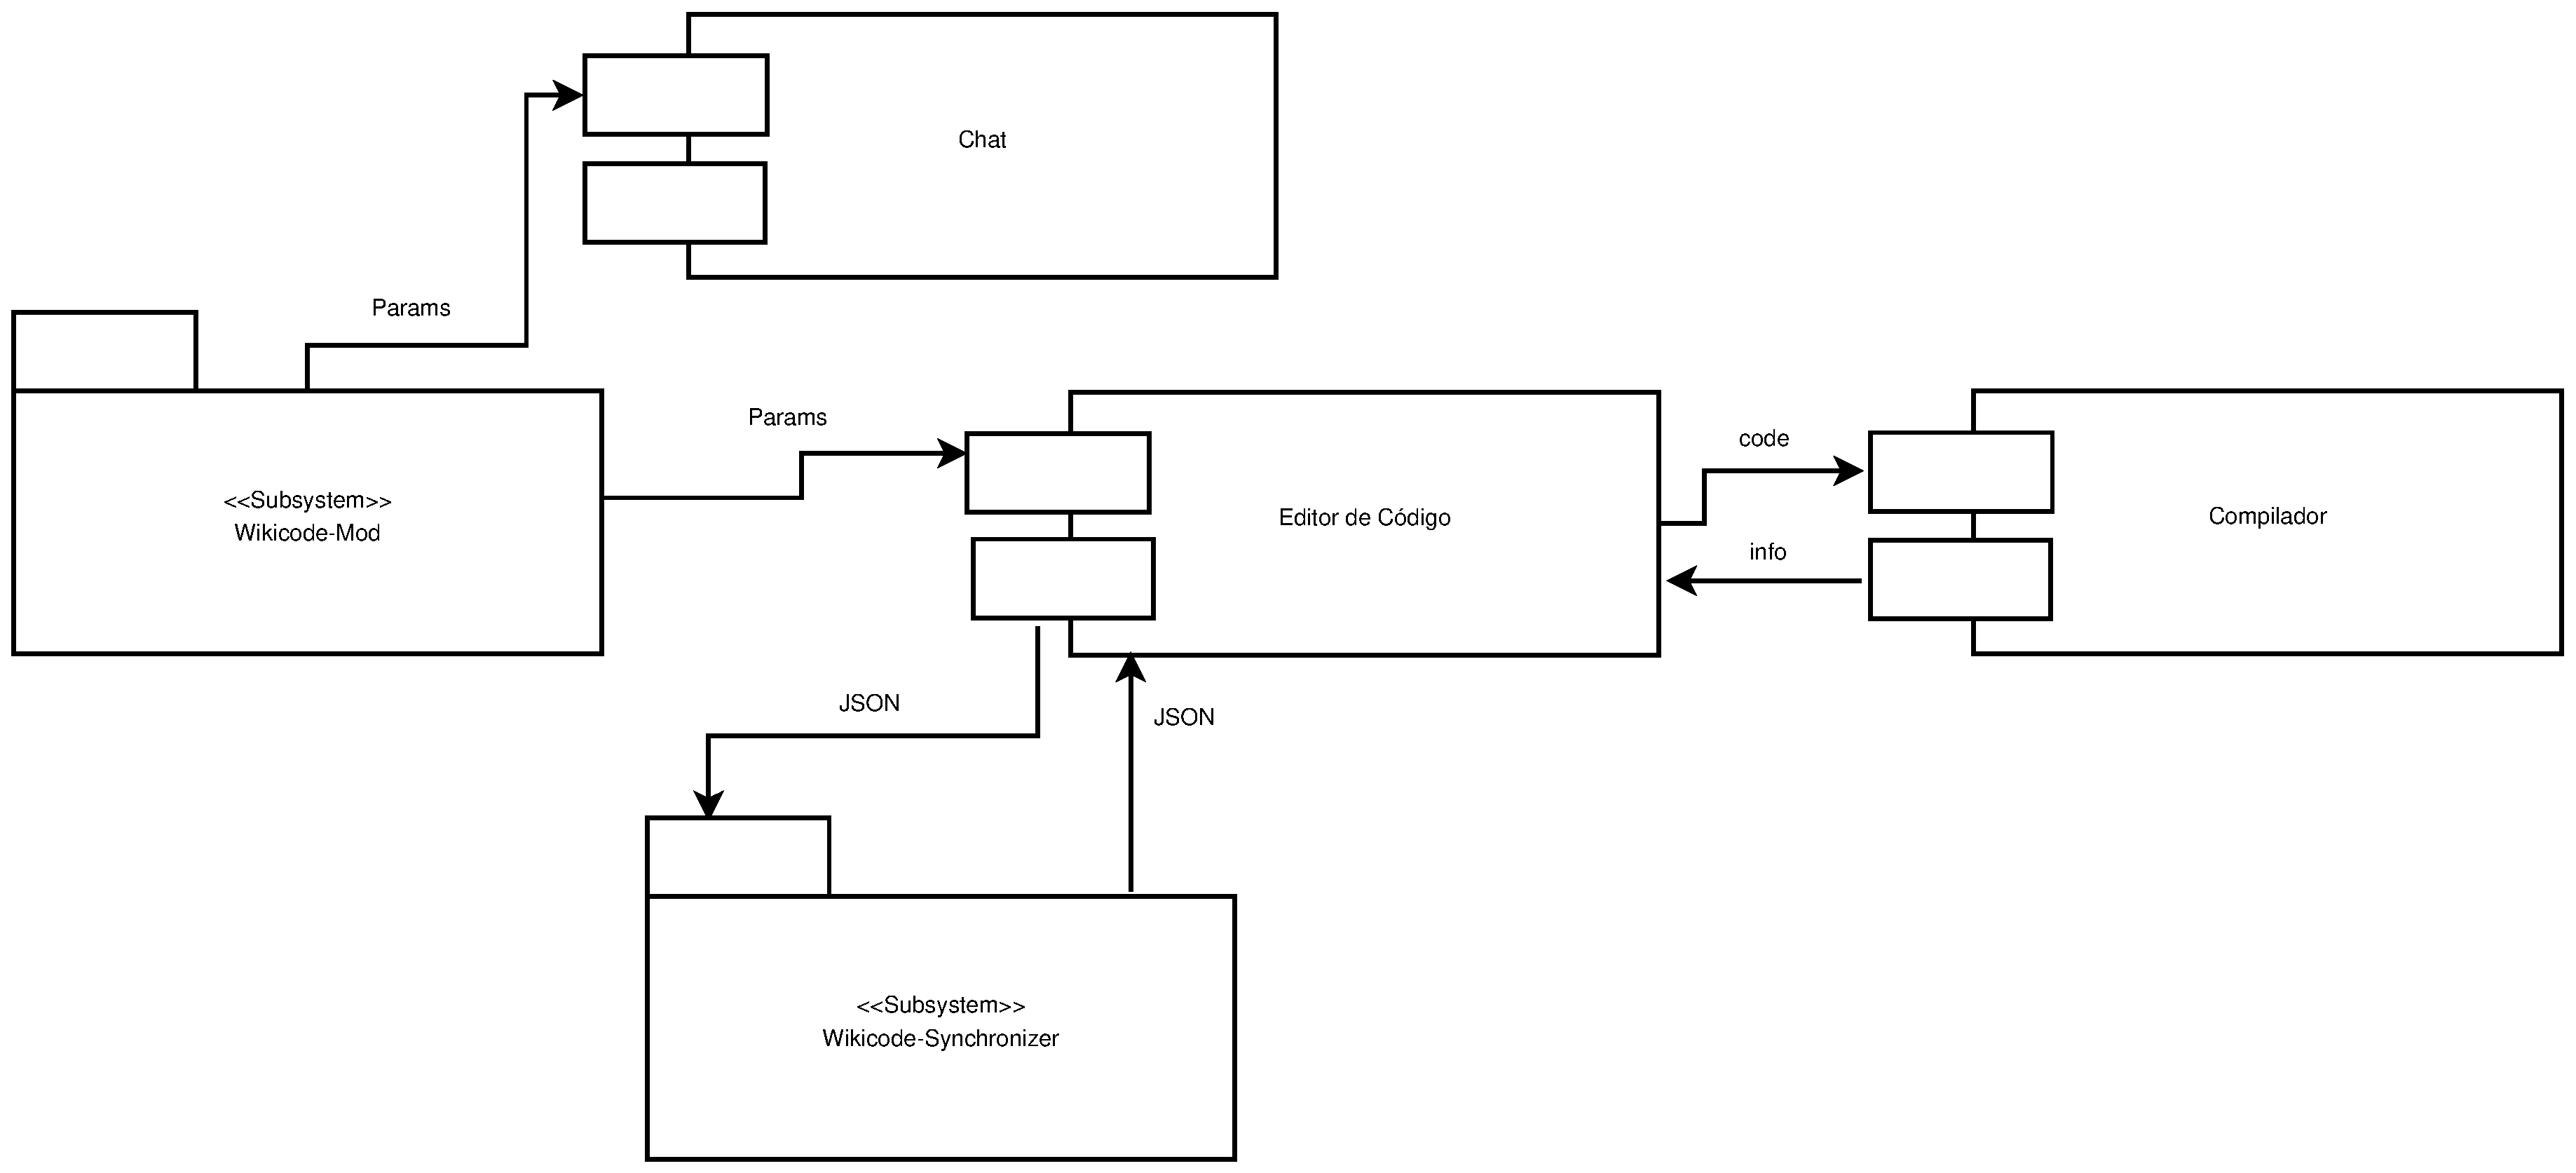
\includegraphics[width=\textwidth]{./img/componentes.eps}
	\caption{Diagrama de Componentes}
\end{figure}
	%!TEX root=./pfc.tex
\chapter[Pruebas del sistema]{Pruebas del sistema}

La fase de pruebas es una fase primordial para garantizar la fiabilidad de un sistema, debido a que representa un último repaso a las especificaciones, al diseño y a la implementación del mismo.
Esta parte de la documentación pretende realizar una descripción de las pruebas realizadas al software desarrollado y cuyos correctos resultados permitirán asegurar que el sistema satisface los requisitos impuestos y cumple con los objetivos deseados de manera robusta y eficiente.

\section{Objetivos de las pruebas}

Las pruebas son una actividad en el desarrollo del software en la cual el sistema o alguno de sus componentes se ejecutarán en circunstancias previamente especificadas, observando y registrando los resultados para realizar una evaluación de algún aspecto. Probar es el proceso de ejecutar un programa con el fin de encontrar errores.

En este caso, la prueba exhaustiva del sistema software con el que se trata resulta perfectamente viable debido a que se pueden probar con facilidad todas las posibilidades de su funcionamiento sin incurrir en ningún error. Por ello se plantean una serie de puntos generales para este proceso:

\begin{itemize}
	\item El objetivo es realizar pruebas que delaten distintos errores con poco tiempo y esfuerzo.
	\item Secundariamente demostraremos con las pruebas qué módulos del software funcionan de acuerdo a las especificaciones y requisitos dados. El comportamiento de la aplicación nos indicará qué grado de fiabilidad tiene el programa y su calidad.
	\item Por último, hay que tener en cuenta que las pruebas no aseguran la falta de defectos. Sin embargo, si todo esto resultara ineficiente, se ha de recordar que tras esta fase de pruebas se lleva a cabo una etapa de explotación del sistema, con la peculiaridad de que éste se dispondrá a funcionar en el entorno propio y real de la aplicación pero bajo la supervisión y controlado por los encargados directos del mismo, pudiendo observar si verdaderamente el programa esta listo para su definitiva aceptación.
\end{itemize}

\section{Diseño de los casos de pruebas}

Analizando las especiales características del software, se llega a la conclusión de que es necesario prestar especial atención a:

\begin{itemize}
	\item Asegurar la comunicación entre el módulo de Moodle y el sistema encargado de sincronizar el código y programar los bloqueos. Esta comunicación es la base del sistema por lo que deben estar completamente sincronizados de manera que cada petición sea servida convenientemente. Además, cada cambio en el editor introducida en el cliente debe ser indicada al servidor para que este se encargue de sincronizarlo con el resto de usuarios.
	\item Garantizar la correcta visualización de las pantallas, fundamentalmente la de edición.
	\item Garantizar el correcto acceso a la base de datos, ya sea para obtener cualquier dato de la comunidad como para almacenar y recuperar los datos referentes a la sincronización del código.
	\item Asegurar que un usuario no puede modificar una parte bloqueada por otro usuario, ya sea por error suyo o problemas en el sistema.
	\item Asegurar el correcto funcionamiento de todas las demás opciones posibles.
\end{itemize}

\section{Pruebas estructurales de la caja blanca}

Aprovechando que tanto Java como PHP permiten una sencilla y cómoda interpretación de código, gracias sobre todo a las potentes herramientas que existen para cada una de ellas y que se comentaron en el apartado de recursos software, se ha ejecutado el código al completo haciendo énfasis en bucles y condiciones forzando dicha ejecución en todas aquellas partes de código que por un motivo u otro no suelen ser accedidas. Gracias a este proceso, se han descubierto algunos fallos en dichas zonas que han sido resueltos convenientemente.

Debido a las características del software que se ha desarrollado, el enfoque de las pruebas que, teóricamente, más errores podrá detectar es el funcional o de la caja negra.

\section{Pruebas funcionales o de la caja negra}

\subsection{Análisis de los valores límites}

Al tratarse de un sistema donde la intercomunicación entre el usuario y este es constante, en este apartado es donde radica el mayor número de pruebas. Como la parte fundamental de este proyecto se trata de un editor, el usuario tiene permitido hacer en él todo lo que desee y prácticamente sin limitación alguna. Sin embargo, para evitar errores se ha impedido al usuario realizar una serie de acciones que podrían poner en peligro la estabilidad del sistema. 

Muchas de estas acciones han sido camufladas como ayuda al usuario, como puede ser por ejemplo que la apertura y cerrado de funciones se hace de modo automático. De este modo, y al ser los bloqueos por funciones, es el sistema el que lo delimita automáticamente y no así el usuario.

Una vez puntualizados estos datos, se van a enumerar una serie de hechos que son candidatos a la realización de pruebas:

\begin{itemize}
	\item Un punto en el que se han hecho pruebas exhaustivas es en el acceso a las partes bloqueadas por otro usuario del código fuente. Asimismo también se ha hecho énfasis en los puntos de sección crítica que puedan concurrir.
	\item Otro punto importante es la llamada al compilador, que al tratarse de una aplicación externa lo hace necesario del uso de ficheros, por lo que se ha evaluado el acceso a estos.
	\item Del mismo modo que el punto anterior también se presta atención al chat, que también trabaja con ficheros, por lo que hay que hacer pruebas exhaustivas para su acceso a estos.
	\item Otras pruebas que se han realizado han sido pruebas a la interfaz del software, es decir, se ha probado que todas las pantallas sean accesibles y que la comunicación entre ellas es eficiente.
\end{itemize}

\section{Pruebas del desarrollador}	
	
Realmente son las pruebas más importantes que se han realizado. Básicamente estas pruebas se han centrado fundamentalmente en tres puntos comentados a continuación.

\subsection{Pruebas con un curso real}	
	
Antes de nada comentar que la utilidad de este software se centra en las comunidades virtuales de aprendizaje en las que la colaboración es su principal objetivo. Si esto no es así, gran parte de la utilidad de esta herramienta se perdería, pues la mayor funcionalidad que expresa es su capacidad de hacer el editor colaborativo en tiempo real. 

Para ello en primer lugar se ha creado un curso en Moodle, dentro del cual un profesor simulado ha ido creado una serie anotaciones y matriculando una serie de alumnos virtuales.

\begin{figure}[h]
	\includegraphics[width=\textwidth]{./img/ej1main.eps}
	\caption{Pantalla principal de un curso Moodle}
\end{figure}
	
Una vez dentro del curso se han creado una serie de Wikicodes diferentes para probar las distintas opciones de configuración. Estas pruebas tienen como principales objetivos:

\begin{itemize}
	\item Realizar una serie de códigos fuentes, tanto individualmente como de modo colaborativo, y luego comprobar si la compilación es correcta.
	\item Si la compilación es errónea, comprobar que las líneas referenciadas son claramente identificadas en el editor dentro de la Wikicode.
	\item Comprobar que todas las acciones que puedan realizarse dentro de un entorno de desarrollo pueden hacerse libremente dentro de una Wikicode, desde la restauración de una versión antigua a desbloquear partes de tu código.
\end{itemize}

Por tanto, dicho curso se ha desarrollado de manera completa y se han creado varios alumnos ficticios los cuales realizaron numerosas aportaciones y colaboraciones en la comunidad. Además, se ha utilizado para probar todas las opciones disponibles intentando barajar todas posibilidades que el usuario podría realizar en el entorno del curso.

\begin{figure}[h]
	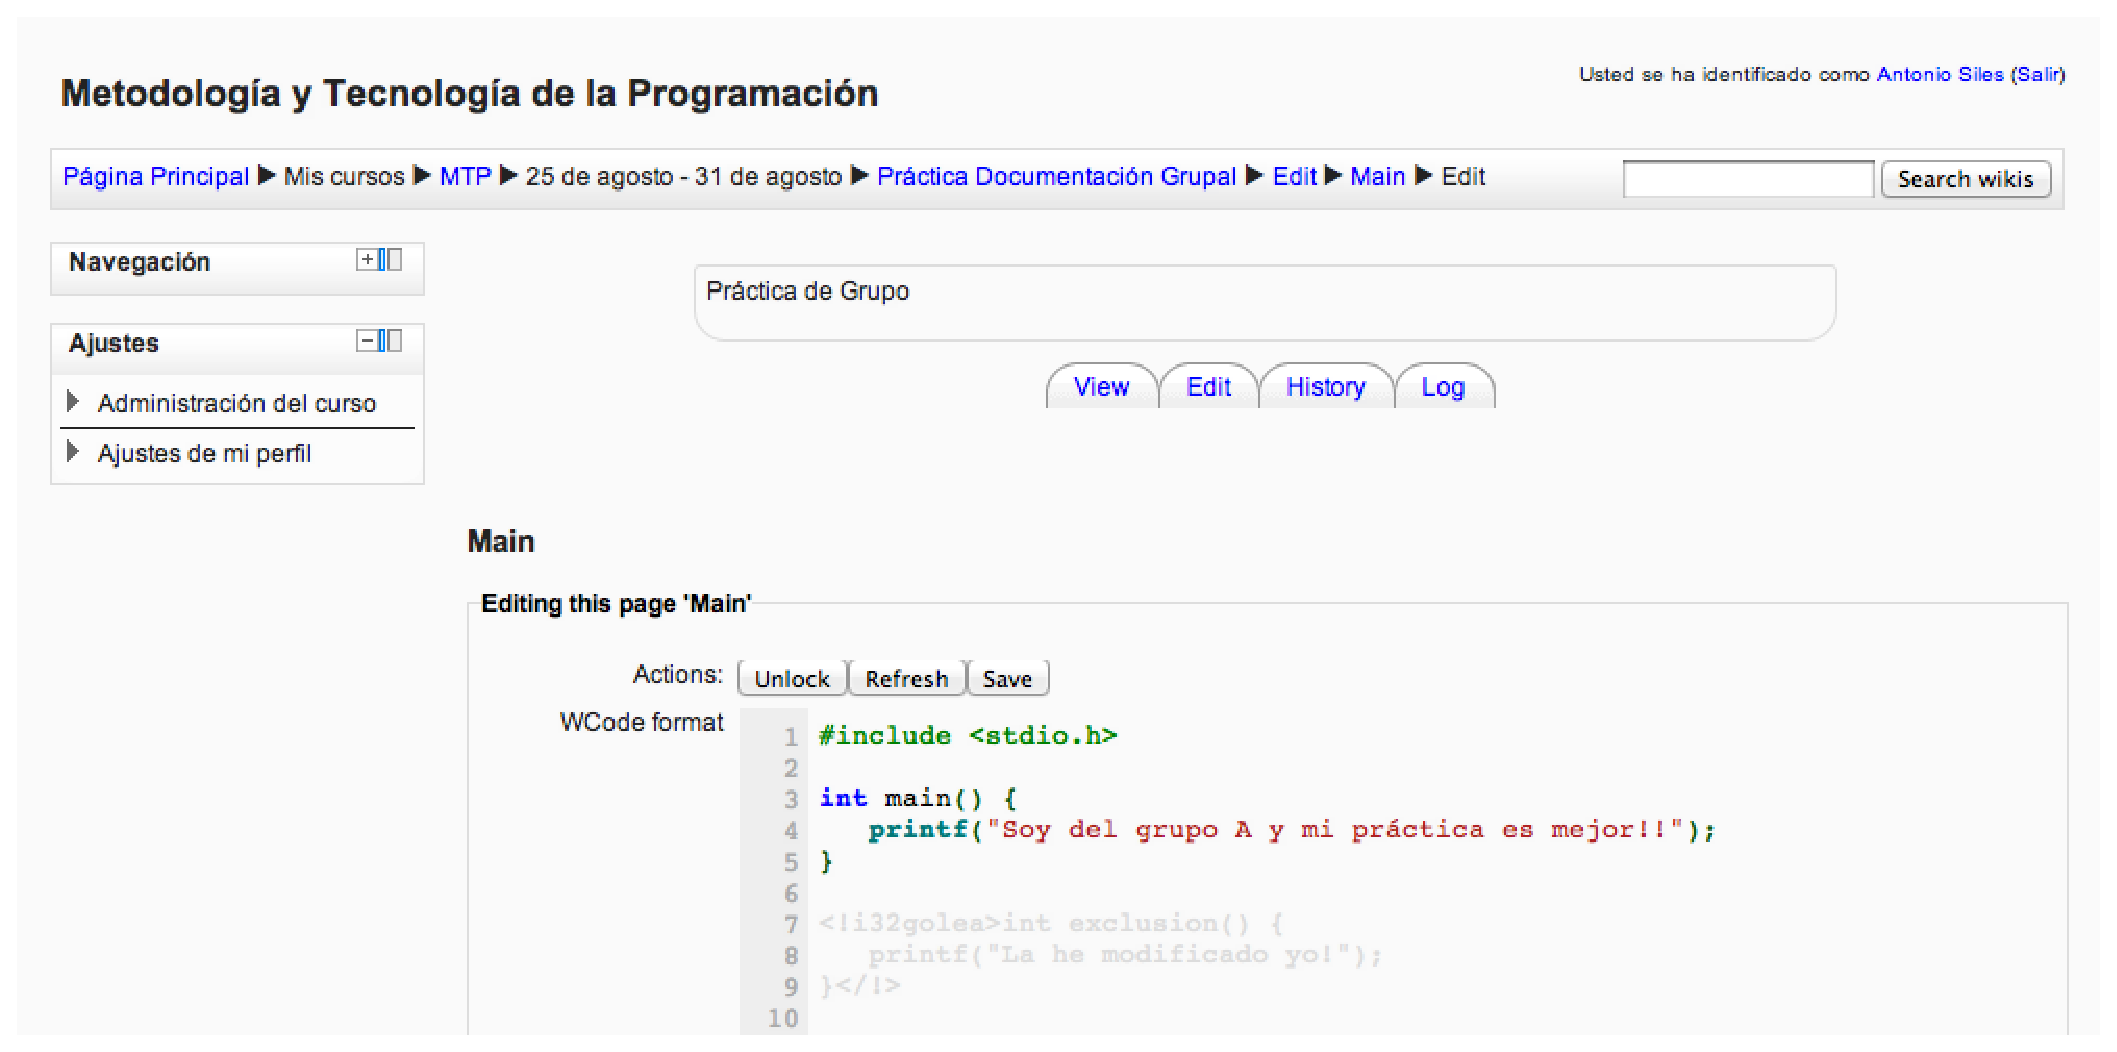
\includegraphics[width=\textwidth]{./img/ej2edit4.eps}
	\caption{Edición de código con una función bloqueada}
\end{figure}

\newpage	
También se ha probado la opción de Descarga del ejecutable una vez compilado y se ha comprobado que se ejecuta correctamente.	
	
\begin{figure}[h]
	\centering
	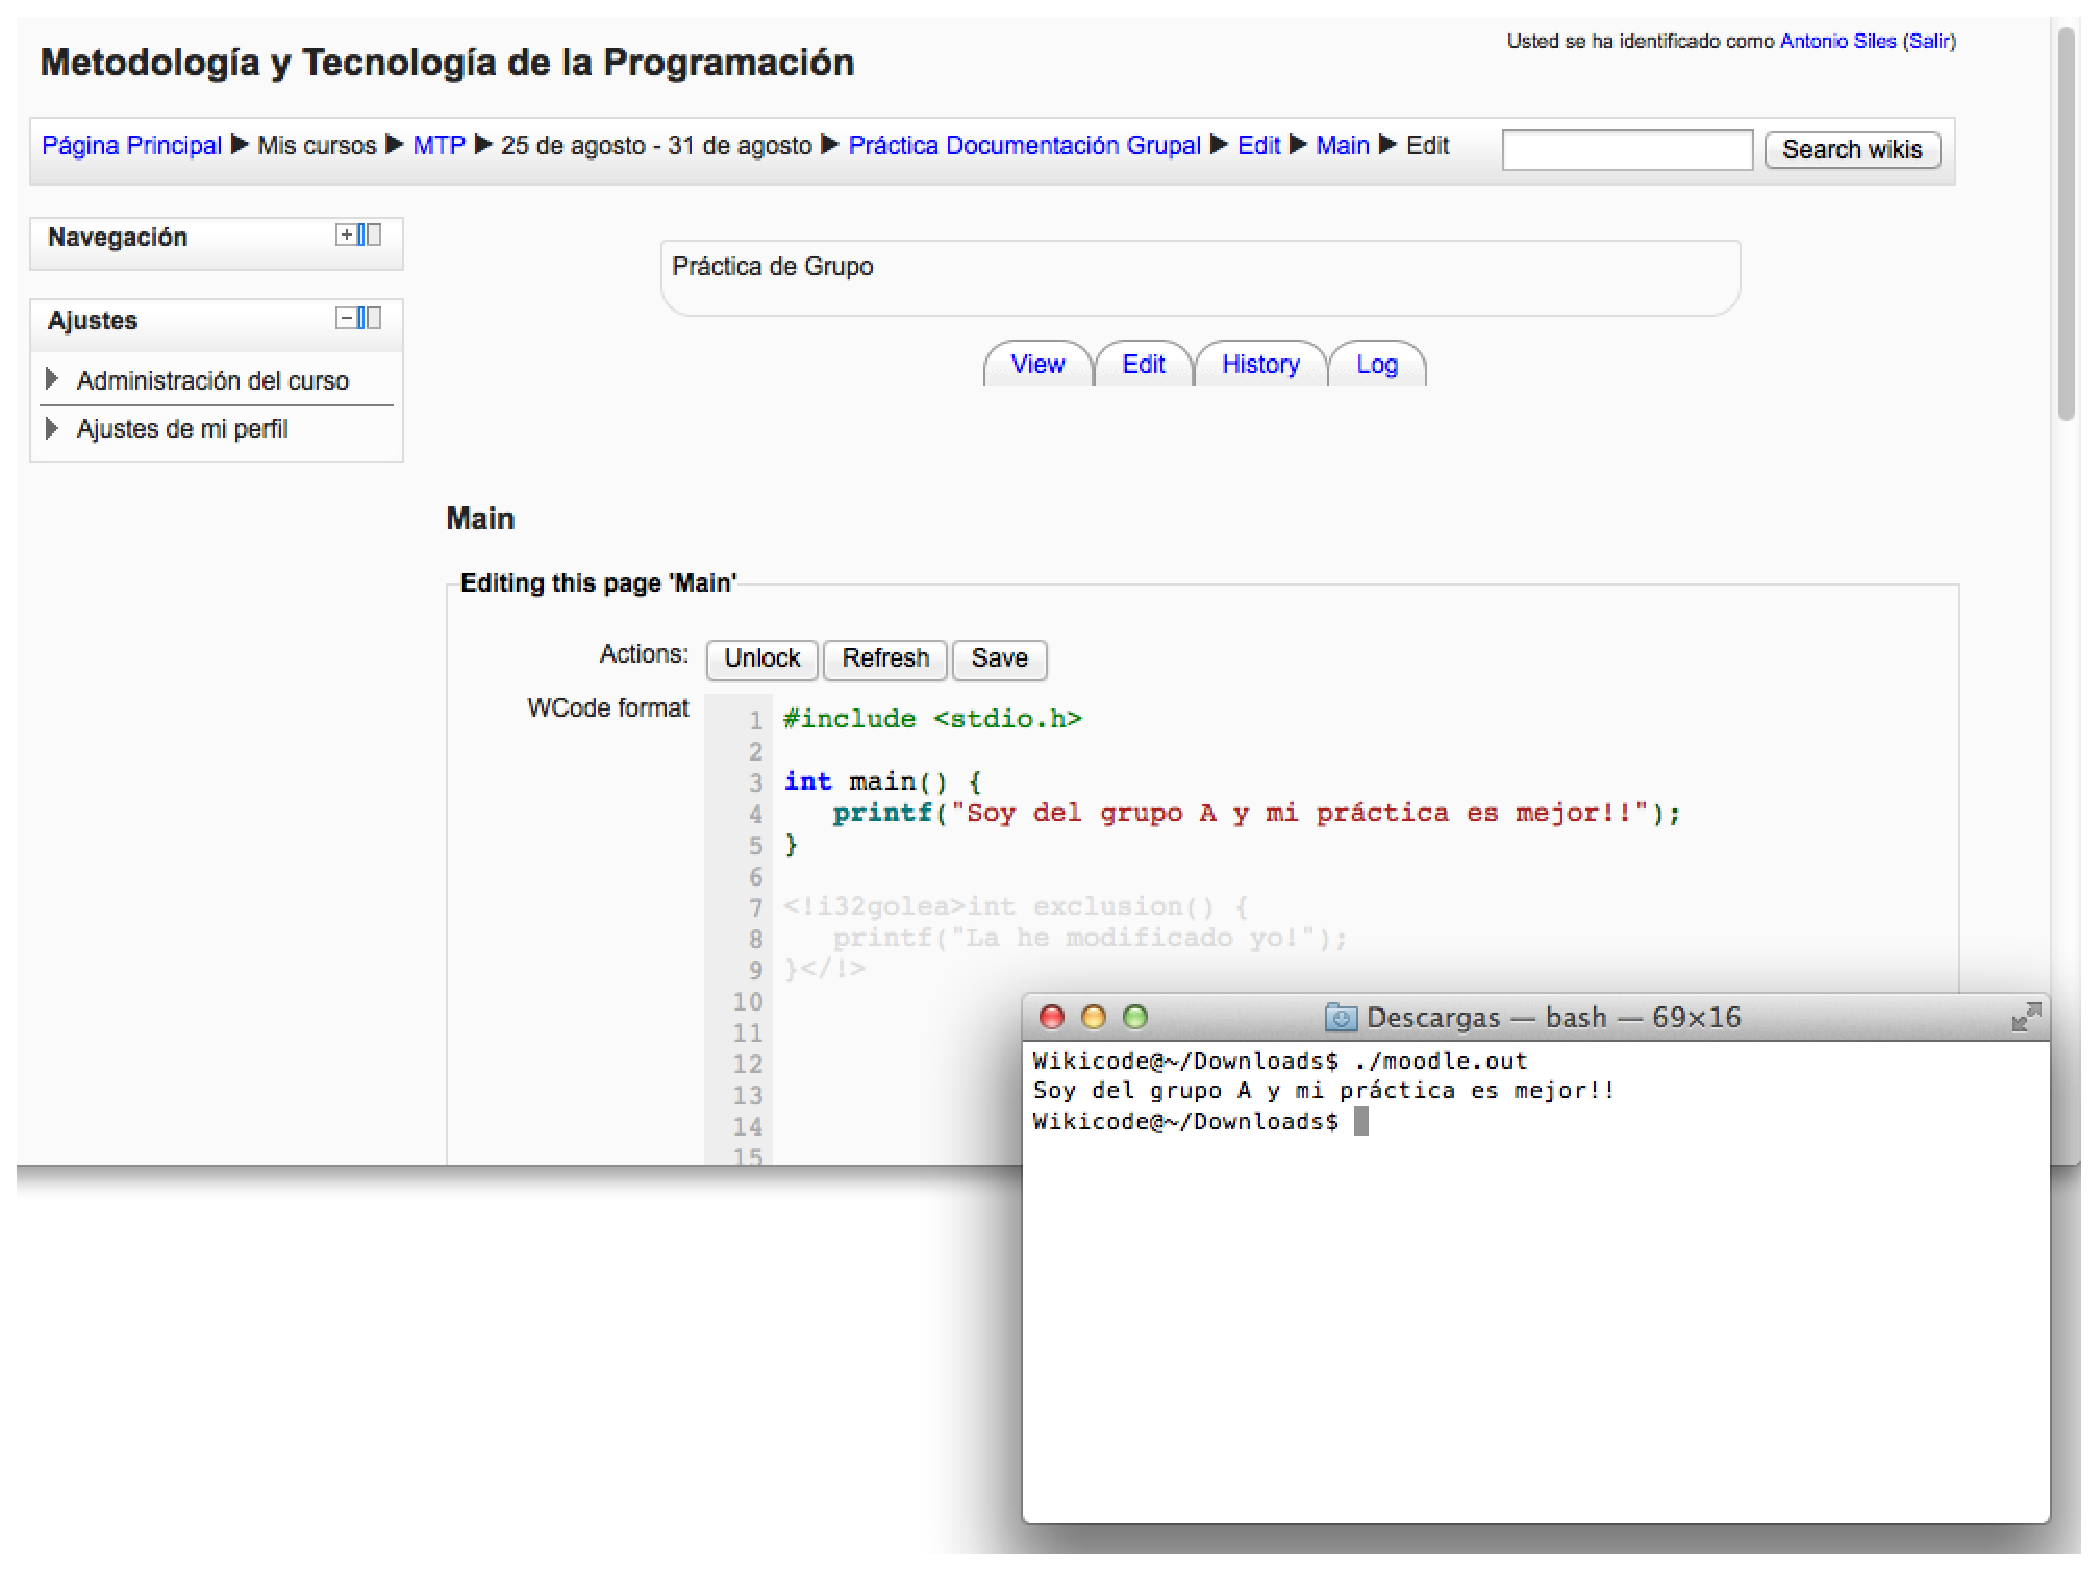
\includegraphics[width=0.9\textwidth]{./img/download.eps}
	\caption{Edición de código. Descarga y ejecución de una aplicación creada.}
\end{figure}	

Por último también se ha comprobado la entrada/salida de texto con respecto al chat que hemos incluido en nuestra plataforma de desarrollo antes de dar el visto bueno a la parte de edición de la plataforma.

\begin{figure}[h]
	\centering
	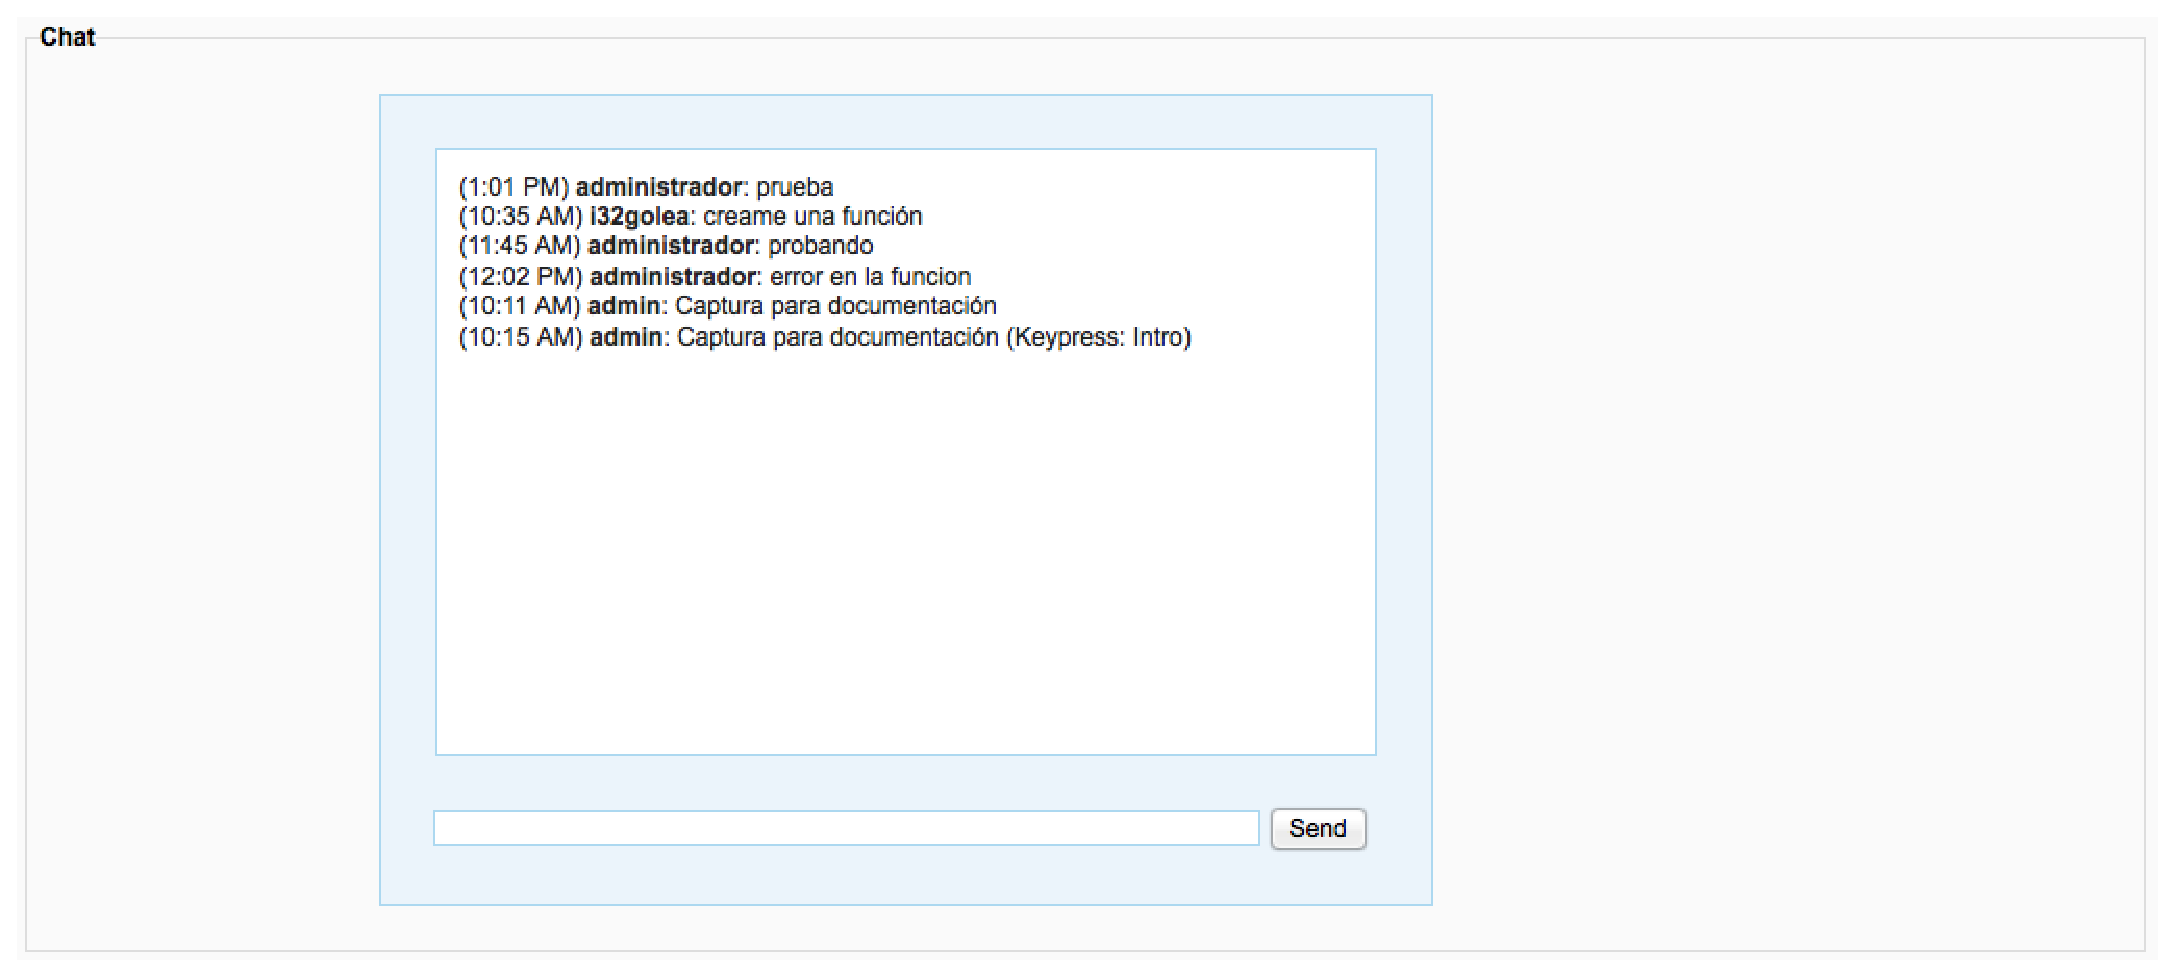
\includegraphics[width=0.65\textwidth]{./img/echat.eps}
	\caption{Edición de código. Chat.}
\end{figure}

\newpage

\subsection{Prueba de compilación utilizando Cross Compiling}
	
Para hacer esta prueba se ha inicializado una máquina virtual con Windows instalado y posteriormente se ha compilado y ejecutado el ejecutable descargado. La salida es la misma que nos ha dado en el sistema operativo nativo de nuestra aplicación por lo que podemos ver que las pruebas realizadas son correctas.
	
\begin{figure}[h]
	\centering
	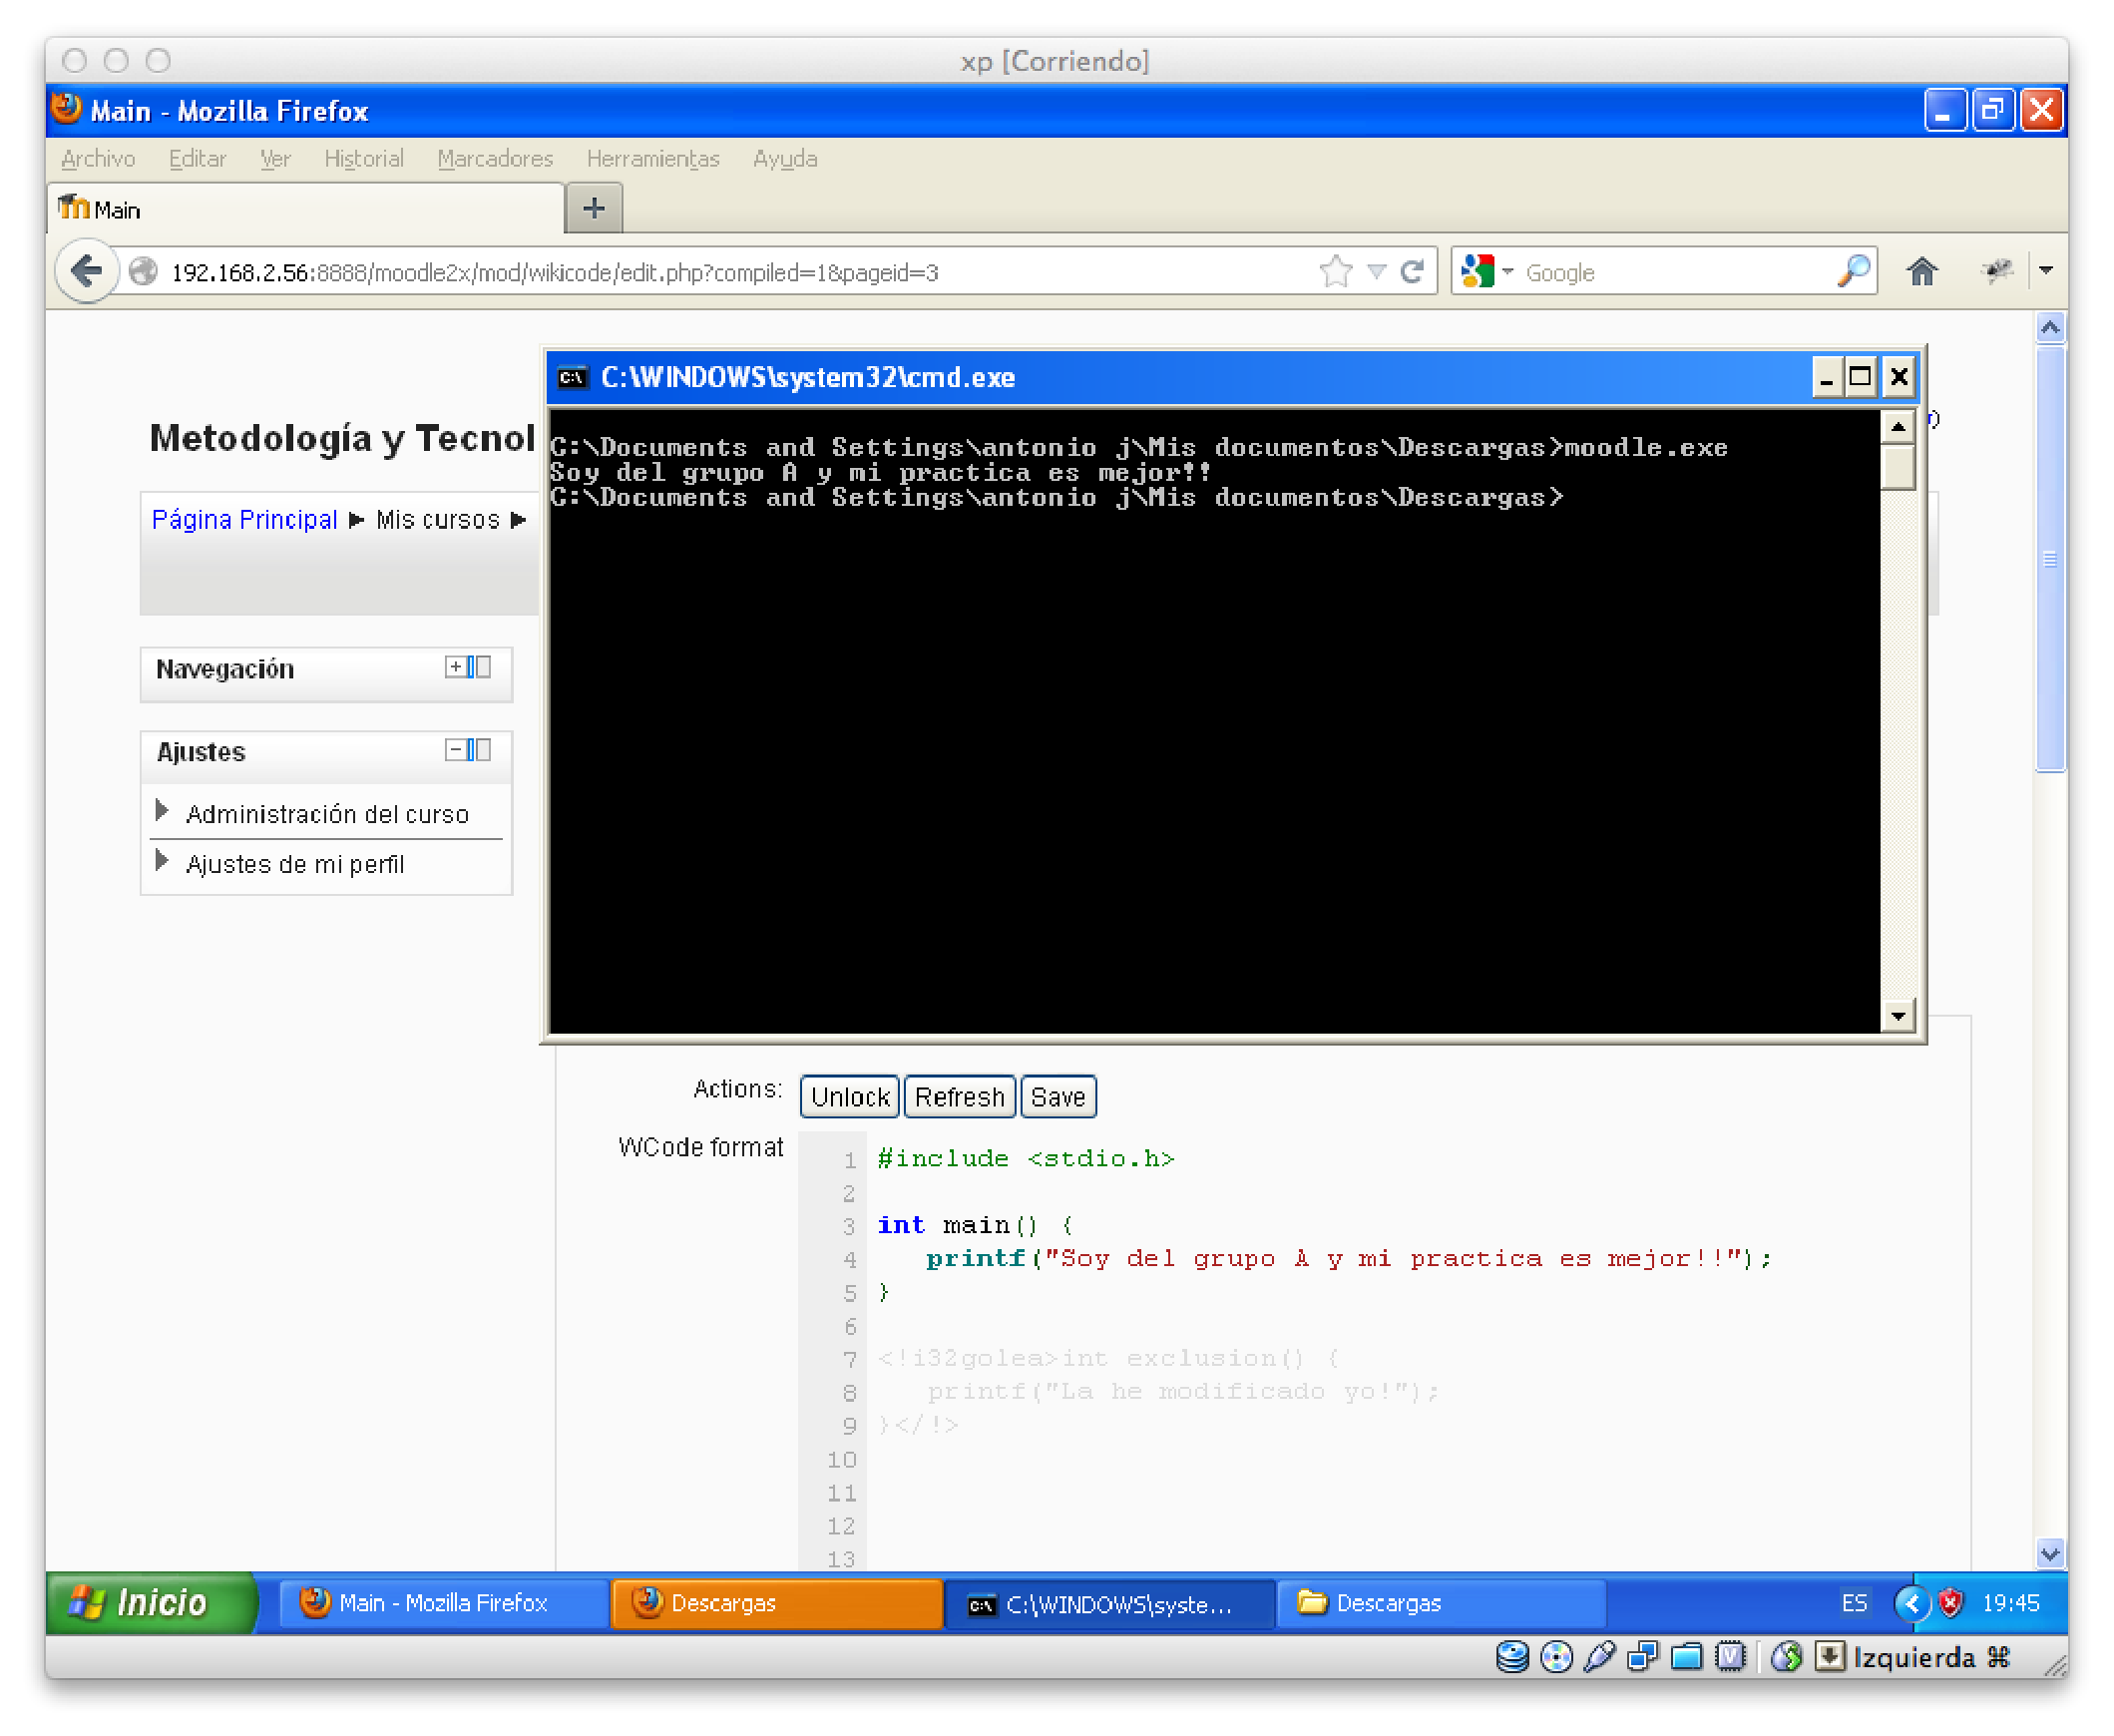
\includegraphics[width=0.9\textwidth]{./img/windows.eps}
	\caption{Edición de código. Cross Compiling.}
\end{figure}		
	
\subsection{Comprobación de estadísticas}
	
Una parte fundamental de Wikicode es su parte estadística, donde el profesor puede comprobar la dificultad que ha tenido un alumno para realizar un determinado código y en función de esto valorar el conocimiento del alumno. Para ello se muestran dos métricas: Número de errores de compilación y Duración de desarrollo del código.

Se han hecho las pruebas oportunas, calculando el tiempo y el número de errores de modo paralelo y comprobando de la veracidad de los hechos.
	
\begin{figure}[h]
	\centering
	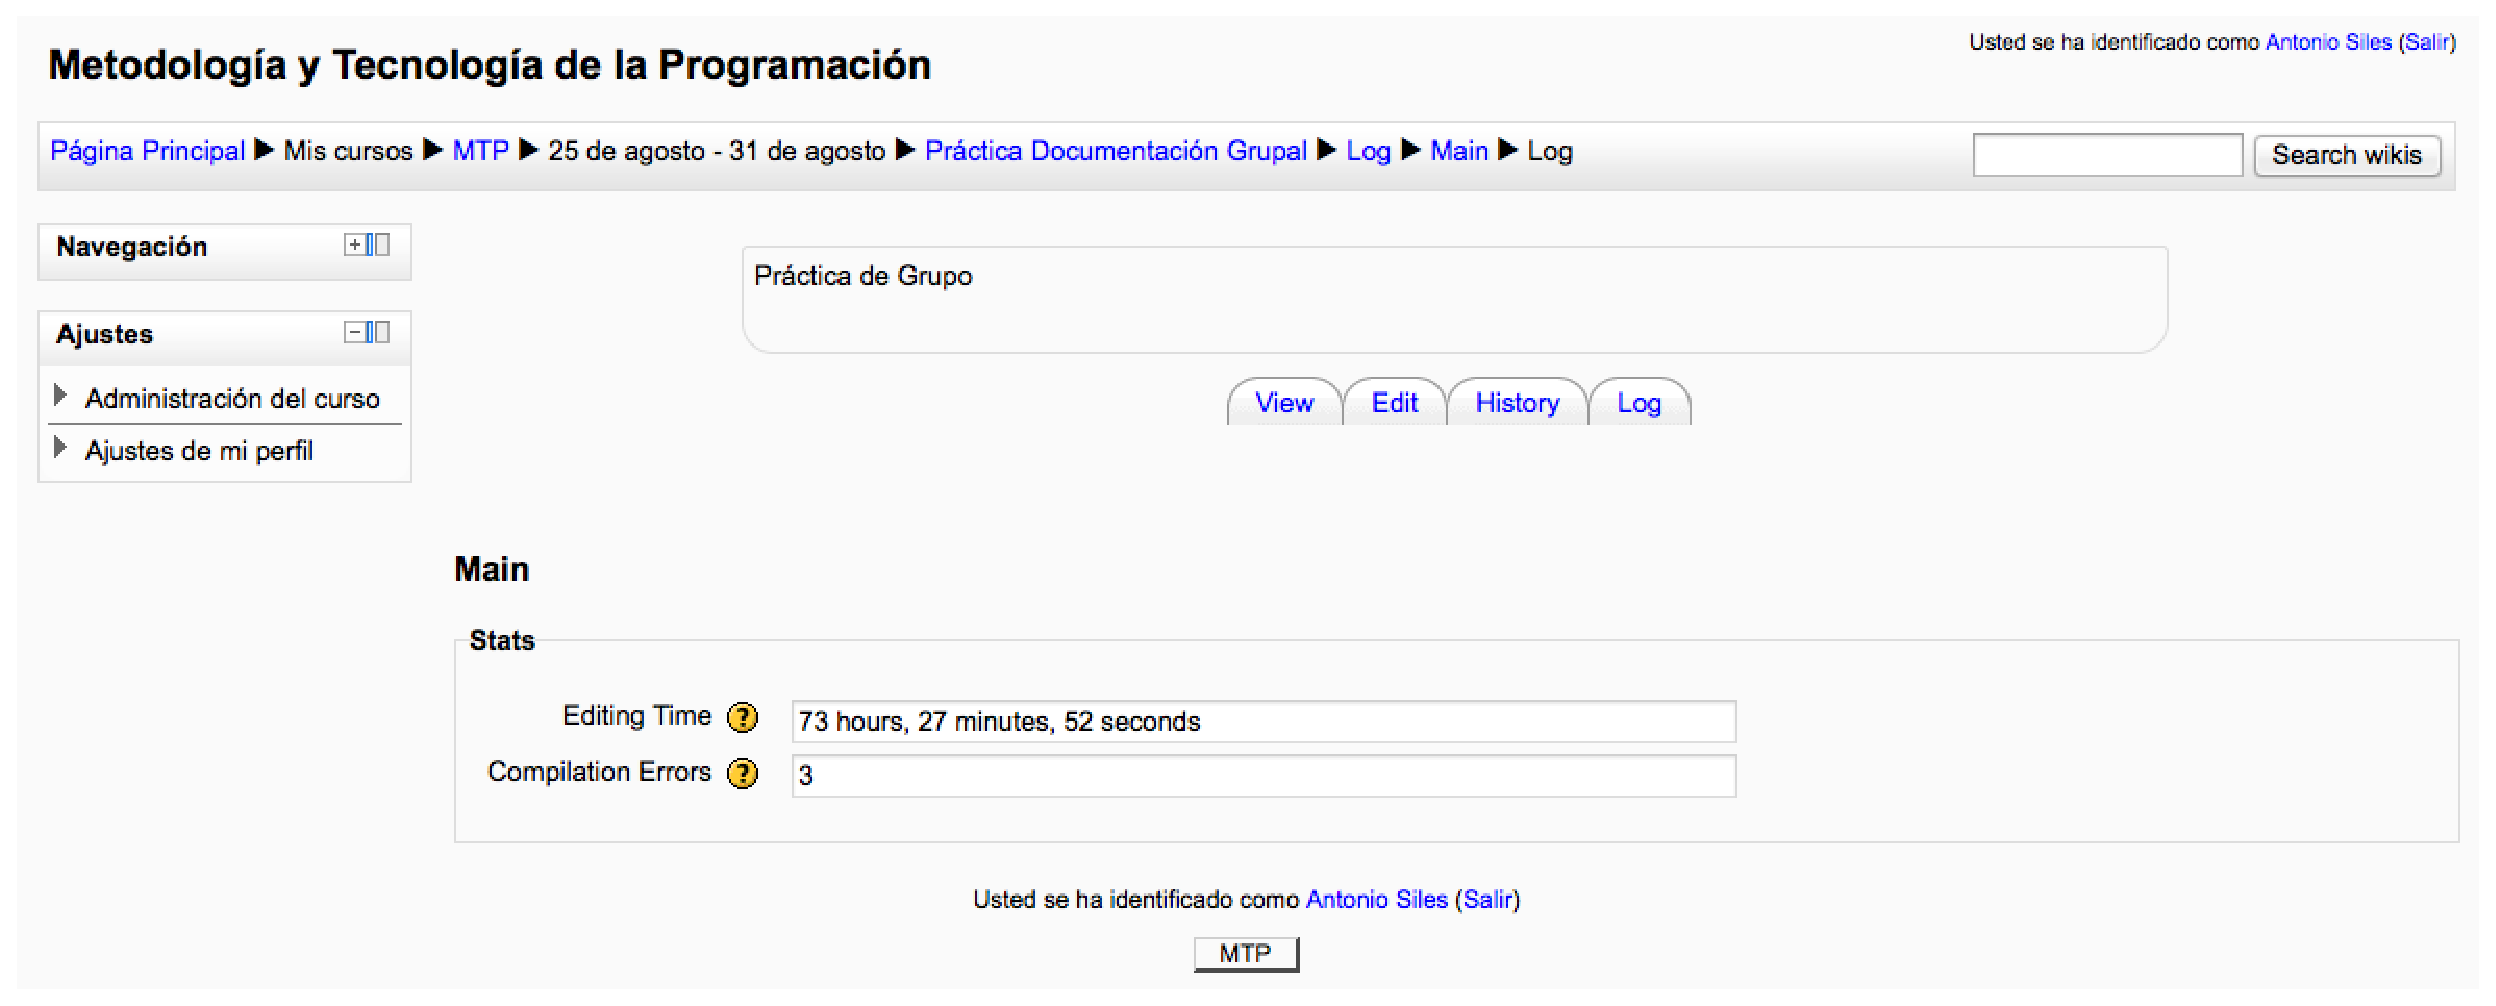
\includegraphics[width=0.9\textwidth]{./img/log.eps}
	\caption{Log de información de una Wikicode.}
\end{figure}

\section{Corrección de errores}

Durante las pruebas se han detectado varios errores de programación, que se han ido corrigiendo conforme se han ido detectando. También se han corregido dos problemas a los que se ha aportado una solución funcional para protección del código, los cuales son los siguientes:

\begin{itemize}
	\item \textbf{Borrado de caracteres especiales}. La aplicación funciona delimitándose por funciones, lo cual nos ayuda a separar los bloqueos unos de otros. Las funciones en el lenguaje de programación C se delimitan por la apertura y cerrado de corchetes, por lo que para eliminar uno de estos caracteres el contenido de su interior ahora deberá de estar vacío. Esto nos impide que el sistema desconozca el dominio de una función.
	\item \textbf{Auto Rollback}. Se ha podido comprobar durante las diversas pruebas que el sistema en caso de error de bloqueos vacía el buffer del código y lo deja en blanco. Se ha modificado la programación de todas las funciones para asegurarnos que siempre que un usuario modifica una función esta esté bloqueada por él, y del mismo modo, por si no se ha detectado algún caso que repercuta en el mismo error se ha programado el sistema de modo que si se vacía el buffer esta acción no se lleve a cabo y restaure el contenido que había anteriormente a la acción que lo ha propiciado.
\end{itemize}

\section{Prueba de aceptación}
	
Esta prueba se ha realizado con varias personas distintas del autor. El uso de la aplicación por parte de esas personas no ha ocasionado ningún error y, por tanto, se puede decir que esta prueba se ha superado de manera satisfactoria.
	
	
	
	
	
	
	
	
	
	
	
	
	
	
	
	
	
	
	
	
	
	
	
	
	
	
	
	
	
	
	
	
	%!TEX root=./pfc.tex
\chapter[Conclusiones y futuras mejoras]{\label{}
Conclusiones y futuras mejoras}

\section{Conclusiones}

El principal objetivo de este proyecto ha sido alcanzado puesto que se ha realizado un editor de código fuente en lenguaje C, colaborativo, e integrado dentro un sistema e-learning. Para este fin se ha conseguir diseñar un módulo compatible con Moodle en todas sus versiones.

De este modo, todos los objetivos referentes al hecho de crear un editor on-line se han cumplido con todas las características de un entorno de desarrollo. También se ha permitido al tutor la configuración de una serie de parámetros que son utilizados a la hora de compilar y desarrollar los códigos fuentes. Estos parámetros nos permiten compilar en cualquier OS que deseemos instalar el sistema así como tener una serie de estadísticas.

Una de las principales ventajas que se han obtenido con el desarrollo de este proyecto es que ahora los alumnos cuentan con una gran herramienta para programar, sin necesidad de tener conocimiento informático alguno y sin necesidad de tener que instalar nada en sus equipos. A la vez, fomenta la colaboración entre los compañeros a la hora de realizar cualquier ejercicio de programación e impide hacer el típico \emph{copy\&paste} para la realización de prácticas. Por otra parte, el profesor cuenta ahora con una herramienta más potente a la hora de evaluar los conocimientos en este área de su alumnado.

Además el back-end\footnote{\textbf{Back-end: }Parte de la aplicación encargada de administrar el sistema.} de la aplicación es totalmente independiente. De este modo, si se deseara exportar a otro sistema e-learning bastaría con diseñar un front-end dentro de ese sistema y enlazar con nuestro sistema. 

Otro de los objetivos cumplidos es la realización de un estudio de los sistemas e-learning más importantes en la actualidad analizando sus pros y sus contras así como realizando una explicación detallada de la elección de Moodle.

En cuanto al diseño de interfaz que se ha utilizado, como realmente lo que se ha desarrollado es un bloque para Moodle y este no tiene mucha complejidad, se ha seguido el mismo estilo gráfico de dicha plataforma. Sin embargo, también se han añadido algunos efectos visuales utilizando técnicas de diseño avanzadas como es el caso del framework JQuery.

\section{Posibles ampliaciones o mejoras}

A continuación se exponen una serie de ampliaciones o mejoras que podrían realizarse en un futuro sobre este sistema:

\begin{itemize}
	\item Se podría aumentar el número de lenguajes de programación disponibles. Ahora mismo el sistema sólo funciona para el lenguaje \textbf{C}, y eso puede limitar la exportación de este módulo para otras asignaturas en las que se enseñe algún otro lenguaje de programación. 
	\item Se puede permitir la realización de proyectos informáticos, dando la posibilidad de manejar varios ficheros en lugar de un único código fuente.
	\item Crear un sistema de importación y exportación de proyectos, de modo que el alumno pueda descargar todos los datos en su equipo para trabajar off-line.
	\item Crear un sistema de ejecución embebido dentro de la propia plataforma de desarrollo, así el alumno no necesitaría descargar el archivo en su equipo para ejecutarlo.
\end{itemize}

	% INCLUIMOS LA BIBLIOGRAFÍA...
	\nocite{*}	% Se usa para indicar en la bibliografía las referencias no citadas.
	\bibliographystyle{alpha}
    	\bibliography{pfc_biblio}

\end{document}

